\documentclass[twoside]{book}

% Packages required by doxygen
\usepackage{fixltx2e}
\usepackage{calc}
\usepackage{doxygen}
\usepackage[export]{adjustbox} % also loads graphicx
\usepackage{graphicx}
\usepackage[utf8]{inputenc}
\usepackage{makeidx}
\usepackage{multicol}
\usepackage{multirow}
\PassOptionsToPackage{warn}{textcomp}
\usepackage{textcomp}
\usepackage[nointegrals]{wasysym}
\usepackage[table]{xcolor}

% Font selection
\usepackage[T1]{fontenc}
\usepackage[scaled=.90]{helvet}
\usepackage{courier}
\usepackage{amssymb}
\usepackage{sectsty}
\renewcommand{\familydefault}{\sfdefault}
\allsectionsfont{%
  \fontseries{bc}\selectfont%
  \color{darkgray}%
}
\renewcommand{\DoxyLabelFont}{%
  \fontseries{bc}\selectfont%
  \color{darkgray}%
}
\newcommand{\+}{\discretionary{\mbox{\scriptsize$\hookleftarrow$}}{}{}}

% Page & text layout
\usepackage{geometry}
\geometry{%
  a4paper,%
  top=2.5cm,%
  bottom=2.5cm,%
  left=2.5cm,%
  right=2.5cm%
}
\tolerance=750
\hfuzz=15pt
\hbadness=750
\setlength{\emergencystretch}{15pt}
\setlength{\parindent}{0cm}
\setlength{\parskip}{3ex plus 2ex minus 2ex}
\makeatletter
\renewcommand{\paragraph}{%
  \@startsection{paragraph}{4}{0ex}{-1.0ex}{1.0ex}{%
    \normalfont\normalsize\bfseries\SS@parafont%
  }%
}
\renewcommand{\subparagraph}{%
  \@startsection{subparagraph}{5}{0ex}{-1.0ex}{1.0ex}{%
    \normalfont\normalsize\bfseries\SS@subparafont%
  }%
}
\makeatother

% Headers & footers
\usepackage{fancyhdr}
\pagestyle{fancyplain}
\fancyhead[LE]{\fancyplain{}{\bfseries\thepage}}
\fancyhead[CE]{\fancyplain{}{}}
\fancyhead[RE]{\fancyplain{}{\bfseries\leftmark}}
\fancyhead[LO]{\fancyplain{}{\bfseries\rightmark}}
\fancyhead[CO]{\fancyplain{}{}}
\fancyhead[RO]{\fancyplain{}{\bfseries\thepage}}
\fancyfoot[LE]{\fancyplain{}{}}
\fancyfoot[CE]{\fancyplain{}{}}
\fancyfoot[RE]{\fancyplain{}{\bfseries\scriptsize Generated by Doxygen }}
\fancyfoot[LO]{\fancyplain{}{\bfseries\scriptsize Generated by Doxygen }}
\fancyfoot[CO]{\fancyplain{}{}}
\fancyfoot[RO]{\fancyplain{}{}}
\renewcommand{\footrulewidth}{0.4pt}
\renewcommand{\chaptermark}[1]{%
  \markboth{#1}{}%
}
\renewcommand{\sectionmark}[1]{%
  \markright{\thesection\ #1}%
}

% Indices & bibliography
\usepackage{natbib}
\usepackage[titles]{tocloft}
\setcounter{tocdepth}{3}
\setcounter{secnumdepth}{5}
\makeindex

% Hyperlinks (required, but should be loaded last)
\usepackage{ifpdf}
\ifpdf
  \usepackage[pdftex,pagebackref=true]{hyperref}
\else
  \usepackage[ps2pdf,pagebackref=true]{hyperref}
\fi
\hypersetup{%
  colorlinks=true,%
  linkcolor=blue,%
  citecolor=blue,%
  unicode%
}

% Custom commands
\newcommand{\clearemptydoublepage}{%
  \newpage{\pagestyle{empty}\cleardoublepage}%
}

\usepackage{caption}
\captionsetup{labelsep=space,justification=centering,font={bf},singlelinecheck=off,skip=4pt,position=top}

%===== C O N T E N T S =====

\begin{document}

% Titlepage & ToC
\hypersetup{pageanchor=false,
             bookmarksnumbered=true,
             pdfencoding=unicode
            }
\pagenumbering{alph}
\begin{titlepage}
\vspace*{7cm}
\begin{center}%
{\Large N\+ES Emulator }\\
\vspace*{1cm}
{\large Generated by Doxygen 1.8.13}\\
\end{center}
\end{titlepage}
\clearemptydoublepage
\pagenumbering{roman}
\tableofcontents
\clearemptydoublepage
\pagenumbering{arabic}
\hypersetup{pageanchor=true}

%--- Begin generated contents ---
\chapter{Emulateur N\+ES}
\label{md_gestion-de-projet_cdcf_cahier-des-charges}
\Hypertarget{md_gestion-de-projet_cdcf_cahier-des-charges}
\subsection*{Presentation du projet}

Ce projet porte sur l\textquotesingle{}émulation du système de la console de jeux \hyperlink{struct_n_e_s}{N\+ES}. C\textquotesingle{}est à dire reproduire son comportement hardware et software de manière logicielle. La console de jeux \hyperlink{struct_n_e_s}{N\+ES} est une console de jeux sortie en 1985 et développée par la société japonaise Nintendo.

\subsection*{Objectifs}


\begin{DoxyItemize}
\item Emuler le fonctionnement de la console \hyperlink{struct_n_e_s}{N\+ES} de Nintendo
\item Être en capacité d\textquotesingle{}émuler la plupart des jeux sous license
\item Développer pour fonctionner sous Linux
\end{DoxyItemize}

\subsection*{Outils de développement}

Nous avons choisi développer notre émulateur à travers un Makefile, de tel manière à ce que chacun puisse utiliser son propre I\+DE (vim, Atom, Code\+Blocks). A l\textquotesingle{}avenir, nous utiliserons C\+Make pour généraliser la compilation et la reprise du projet sur n\textquotesingle{}importe quel I\+DE.

\subsection*{Comment fonctionne la \hyperlink{struct_n_e_s}{N\+ES}}

\subsubsection*{\hyperlink{struct_c_p_u}{C\+PU}}

\paragraph*{Representation de la mémoire}



\paragraph*{Fonctionnement du processeur 6502}

Le processeur est de type 8 bits. Ses registres de travail sont donc aussi de taille 8 bits. Cela implique que c\textquotesingle{}est aussi la taille maximale des données manipulables.

Cependant, le Programme Counter (PC) est lui de taille 16 bits. Le domaine d\textquotesingle{}adressage disponible est ainsi de 64\+Ko.

Il possède en plus un Multi-\/\+Memory \hyperlink{struct_controller}{Controller} (M\+MC) qui permet d\textquotesingle{}adresser plus de mémoire. (Voir partie mémoire).

Le processeur possède un jeu d\textquotesingle{}instruction capable de manipuler les 64 Ko de mémoire et 6 registres.

{\bfseries Registres 8 bits} \+:
\begin{DoxyItemize}
\item {\bfseries \hyperlink{struct_stack}{Stack} register} \+: Garde l\textquotesingle{}adresse du haut de la pile, pile permettant de sauvegarder des données lors de l’exécution d\textquotesingle{}une fonction.
\item {\bfseries Processor Status} \+: Registre de flags, il possède en tout 7 flags car le bit numéro 5 du registre n\textquotesingle{}est pas utilisé.
\begin{DoxyItemize}
\item Bit 0 \+: Carry out (C)
\item Bit 1 \+: Zero flag (Z)
\item Bit 2 \+: Interrupt Disable Flag (I)
\item Bit 3 \+: Decimal mode (D)
\item Bit 5 \+: N/A
\item Bit 6 \+: Break Command (B)
\item Bit 7 \+: Negative Flag (N)
\end{DoxyItemize}
\item {\bfseries Accumulator} \+: Registre de travail principal. Utilisé pour toutes les instructions arithmétiques et logiques.
\item {\bfseries Registre X} \+: Utilisé pour les adressages indexés et le contrôle des boucles.
\item {\bfseries Registre Y} \+: Comparable au registre X mais possède moins de fonctionnalités.
\end{DoxyItemize}

{\bfseries Registres 16 bits}
\begin{DoxyItemize}
\item Program Counter \+: Adressage des 64 Ko de mémoire. Il contient l\textquotesingle{}adresse de la prochaine instruction à exécuter.
\end{DoxyItemize}

\paragraph*{Les modes d\textquotesingle{}adressages}

Le processeur 6502 possède 12 modes d\textquotesingle{}adressage utilisés par les instructions.


\begin{DoxyItemize}
\item Adressage immédiat \+: \#\$??
\item Adressage absolu \+: \$????
\item Adressage page zéro \+: \$??
\item Adressage indirect absolu \+: (\$????)
\item Adressage absolu indexé \+: \$????,X
\item Adressage indexé page zéro \+: \$??,X
\item Adressage indexé indirect \+: (\$??,X)
\item Adressage indirect indexé \+: (\$??),X
\item Adressage relatif \+: \$?? -\/$>$signé
\item Adressage implié \+: transparent dans l\textquotesingle{}instruction
\end{DoxyItemize}

\paragraph*{Les instructions}

Le processeur possède un jeu de 56 mnémoniques (instructions). Certaines peuvent faire l\textquotesingle{}objet de plusieurs modes d\textquotesingle{}adressage.

{\bfseries Exemple de deux instructions}

{\bfseries A\+DC} \+: Flags utilisés \+: N,Z,C,V

Additionne la valeur contenu dans l\textquotesingle{}Accumulator avec l\textquotesingle{}opérande désigné par le mode d\textquotesingle{}adressage et le bit de retenue. Le résultat est ensuite placé dans l\textquotesingle{}Accumulator. Il y a aussi une mise à jour des flags. Pour effectuer une addition vierge, il faut mettre à zéro le bit de retenue (C). Cette instruction peut utiliser 8 modes d\textquotesingle{}adressage différents.

{\bfseries L\+DA} -\/ Load Accumulator \+: Flags Utilisés \+: N,Z

On passe en paramètre une adresse. L\textquotesingle{}opérande situé à cette adresse en mémoire centrale est chargé dans l\textquotesingle{}Accumulator puis la valeur est évaluée pour déterminer les flags N et Z.

\subsubsection*{\hyperlink{struct_p_p_u}{P\+PU}}

La \hyperlink{struct_p_p_u}{P\+PU} (Picture Processing Unit) a pour fonction de gérer l\textquotesingle{}affichage. La résolution des images produites sont de 256x240 pixels. Son fonctionnement est parallèle et indépendant de la \hyperlink{struct_c_p_u}{C\+PU}. Ainsi, la \hyperlink{struct_p_p_u}{P\+PU} possède son propre espace d\textquotesingle{}adressage.

\paragraph*{Frame rendering}

Le rendu des images/frames s\textquotesingle{}exécute à 60 Hz pour une \hyperlink{struct_n_e_s}{N\+ES} N\+T\+SC et 50 Hz pour la version P\+AL. La \hyperlink{struct_p_p_u}{P\+PU} fonctionne avec une fréquence d\textquotesingle{}horloge 3 fois supérieure à celle de la \hyperlink{struct_c_p_u}{C\+PU}, ainsi {\bfseries 3 pixels sont rendus à l\textquotesingle{}écran en un cycle \hyperlink{struct_c_p_u}{C\+PU}}. On appelle scanline le rendu d\textquotesingle{}une ligne de pixels, comprenant également les pixels invisibles nécessaires au timing des signaux composites. Ainsi on décompte 262 scanlines, chacune d\textquotesingle{}entre elles étant composée de 341 pixels. Lorsque la \hyperlink{struct_p_p_u}{P\+PU} a fini de rendre l\textquotesingle{}image visible à l\textquotesingle{}écran, une succession de 20 scanlines prend place, on appelle cet période {\bfseries vertical blank}. C\textquotesingle{}est durant cet période que l\textquotesingle{}on doit écrire dans la mémoire vidéo pour éviter de potentiels artefacts.

\paragraph*{Pattern Tables}

Pour pallier aux contraintes de l\textquotesingle{}époque, les données décrivant les informations à l\textquotesingle{}écran sont grossières \+: on ne stocke pas en brut la couleur d\textquotesingle{}un pixel à des coordonnées précises, à la place, on crée des blocs contenant les informations nécessaires (dessin, couleur) puis on vient les appeler dans une table mémoire pour les afficher à l\textquotesingle{}écran. Un bloc élémentaire est constitué de {\bfseries 8x8 pixels} et est appelé {\bfseries fun pattern}. Ces patterns permettent de décrire le décor (background) et les personnages/objets à l\textquotesingle{}écran (sprites).

La table des patterns est contenue dans une R\+OM (appelé C\+H\+R-\/\+R\+OM) sur le circuit imprimé de la cartouche de jeu. Cette R\+OM est généralement d\textquotesingle{}une taille de 8\+KB, permettant de {\bfseries stocker 512 patterns}. Chaque pattern occupe 16 octets de mémoire, décrivant ainsi les couleurs avec deux bits par pixels, {\bfseries soit 4 couleurs possibles pour sur un pattern} (voir l\textquotesingle{}illustration ci-\/dessous). Nous verrons dans la partie sur les palettes de couleur comment fonctionne le mécanisme de coloriage.



La figure ci-\/dessous illustre le contenu de la table des patterns pour le jeu Super Mario Bros. On retrouve des élements de background comme des sprites.



\paragraph*{Colour Palette}

La \hyperlink{struct_n_e_s}{N\+ES} est capable d\textquotesingle{}afficher {\bfseries 52 couleurs}, cependant, dû aux limitations techniques de l\textquotesingle{}époque, seulement quelques couleurs pourront être affichées sur une frame. L\textquotesingle{}objectif de cette limitation est de limiter l\textquotesingle{}espace mémoire qu\textquotesingle{}occuperont les images. Ainsi, la solution fut de créer {\bfseries des palettes de 4 couleurs} \+: {\bfseries 4 palettes pour le background et 4 autres pour les sprites}. Les éléments affichés à l\textquotesingle{}écran feront référence à une des palettes de couleurs (grâce à un index) afin d\textquotesingle{}être coloriés correctement.

Sur l\textquotesingle{}illustration qui suit, les quatre palettes du haut correspondent aux palettes pour les sprites. On remarque pour chacun d\textquotesingle{}eux que la dernière couleur semble être noire, or en réalité il s\textquotesingle{}agit de {\bfseries la transparence} \+: un pixel possédant cet priorité laisse entrevoir le background. Juste en dessous, on retrouve les palettes pour le background.



\paragraph*{Name Tables}

Le background est constitué {\bfseries d\textquotesingle{}une grille de 32x30 patterns}. En mémoire, on appelle cet grille/tableau une {\bfseries name table}. On associe à cet espace une {\bfseries attribute table}, une table permettant de décrire quelle palette de couleur utiliser pour chaque pattern. L\textquotesingle{}espace d\textquotesingle{}adressage de la \hyperlink{struct_p_p_u}{P\+PU} permet {\bfseries l\textquotesingle{}usage de 4 name tables}, ceci-\/dit, seulement deux sont physiquement présentes sur la \hyperlink{struct_n_e_s}{N\+ES}, les deux autres doivent provenir de la cartouche si nécessaire.

L\textquotesingle{}usage de multiple name tables permet d\textquotesingle{}effectuer du {\bfseries scrolling}, principe utilisé dans les jeux de plateformes pour se déplacer dans un niveau (comme dans Super Mario Bros. par exemple).



En fonction de comment le joueur évolue sur la carte (verticalement ou horizontalement), il est possible d\textquotesingle{}organiser les name tables très précisément avec le principe de \href{https://wiki.nesdev.com/w/index.php/Mirroring}{\tt {\bfseries mirroring}}.

\paragraph*{Object Attribute Memory}

La \hyperlink{struct_n_e_s}{N\+ES} est capable d\textquotesingle{}afficher 64 sprites sur une même frame. Cet caractéristique est toutefois contraintes par la limite de {\bfseries 8 sprites par scanline}. Dans le cas d\textquotesingle{}un overflow de sprite sur une scanline, un bit est levé dans les registres d\textquotesingle{}états de la \hyperlink{struct_p_p_u}{P\+PU}. Les informations sur les sprites affichés à l\textquotesingle{}écran sont à écrire dans l\textquotesingle{}Object Attribute Memory (O\+AM) ou aussi appelé S\+P\+R-\/\+R\+AM (sprite R\+AM). Cet espace mémoire est {\bfseries remis à zéro à chaque fois qu\textquotesingle{}une image a été rendue à l\textquotesingle{}écran}, ainsi, le jeu doit réécrire à chaque rendu pour que les sprites puissent être ré-\/affichés à l\textquotesingle{}écran.

Chaque sprite est représenté par 4 octets dans l\textquotesingle{}O\+AM \+:
\begin{DoxyItemize}
\item Position sur l\textquotesingle{}axe Y (bytes 0)
\item Index du pattern à afficher (bytes 1)
\item Attribut du sprite (bytes 2)
\begin{DoxyItemize}
\item Palette de couleur utilisée
\item Priorité du sprite vis-\/à-\/vis du background
\item Mirroir horizontal
\item Mirroir vertical
\end{DoxyItemize}
\item Position sur l\textquotesingle{}axe X (bytes 3)
\end{DoxyItemize}

La priorité entre les différents sprites est gérée par l\textquotesingle{}ordre dans lequel les sprites sont écris dans l\textquotesingle{}O\+AM.

L\textquotesingle{}O\+AM peut être intégralement {\bfseries écrit en D\+MA} depuis le \hyperlink{struct_c_p_u}{C\+PU}, généralement après chaque vertical blank, dans le handler de l\textquotesingle{}interruption N\+MI.

\subsubsection*{A\+PU}

L\textquotesingle{}A\+PU est l\textquotesingle{}unité de traitement sonore de la \hyperlink{struct_n_e_s}{N\+ES}. Cette unité est intégrée à la puce 6502 et communique avec la \hyperlink{struct_c_p_u}{C\+PU} par l\textquotesingle{}intermédiaire de registres. La \hyperlink{struct_c_p_u}{C\+PU} va donc écrire les informations que l\textquotesingle{}A\+PU interprètera et traduira en signal sonore.

Cette unité possède 5 canaux sonores\+:

\tabulinesep=1mm
\begin{longtabu} spread 0pt [c]{*{3}{|X[-1]}|}
\hline
\rowcolor{\tableheadbgcolor}\PBS\centering \textbf{ Nom }&\PBS\centering \textbf{ Type de signal }&\textbf{ Utilisation principale  }\\\cline{1-3}
\endfirsthead
\hline
\endfoot
\hline
\rowcolor{\tableheadbgcolor}\PBS\centering \textbf{ Nom }&\PBS\centering \textbf{ Type de signal }&\textbf{ Utilisation principale  }\\\cline{1-3}
\endhead
\PBS\centering Pulse 1 &\PBS\centering Carré &Mélodie 1 \\\cline{1-3}
\PBS\centering Pulse 2 &\PBS\centering Carré &Mélodie 2 \\\cline{1-3}
\PBS\centering Triangle &\PBS\centering Triangle &Basse \\\cline{1-3}
\PBS\centering Noise &\PBS\centering Aléatoire &Percussions et effets divers \\\cline{1-3}
\PBS\centering D\+MC &\PBS\centering Samples pré-\/enregistrés &Sons pré-\/enregistrés (bonus, pièces, ...) \\\cline{1-3}
\end{longtabu}
À chaque canal correspond des registres décrivant les différentes caractéristiques du son à produire. Ces registres occupent les adresses {\itshape 0x4000} à {\itshape 0x4017}\+:

\tabulinesep=1mm
\begin{longtabu} spread 0pt [c]{*{2}{|X[-1]}|}
\hline
\rowcolor{\tableheadbgcolor}\textbf{ Registres }&\PBS\centering \textbf{ Canal  }\\\cline{1-2}
\endfirsthead
\hline
\endfoot
\hline
\rowcolor{\tableheadbgcolor}\textbf{ Registres }&\PBS\centering \textbf{ Canal  }\\\cline{1-2}
\endhead
{\bfseries 0x4000 -\/ 0x4003} &\PBS\centering Pulse 1 \\\cline{1-2}
{\bfseries 0x4004 -\/ 0x4007} &\PBS\centering Pulse 2 \\\cline{1-2}
{\bfseries 0x4008 -\/ 0x400B} &\PBS\centering Triangle \\\cline{1-2}
{\bfseries 0x400C -\/ 0x400F} &\PBS\centering Noise \\\cline{1-2}
{\bfseries 0x4010 -\/ 0x4013} &\PBS\centering D\+MC \\\cline{1-2}
{\bfseries 0x4015} &\PBS\centering Tous \\\cline{1-2}
{\bfseries 0x4017} &\PBS\centering Tous \\\cline{1-2}
\end{longtabu}
Le registre {\itshape 0x4015} régit l\textquotesingle{}activation ou non des différents canaux. Le registre {\itshape 0x4017} régit le mode du séquenceur (mode 4 état ou mode 5 états, il ne sera pas détaillé ici).

Afin d\textquotesingle{}observer en détail les valeurs dans ces registres, prennons pour exemple, le premier registre utilisé par le canal {\itshape Pulse 1} \+:

\tabulinesep=1mm
\begin{longtabu} spread 0pt [c]{*{3}{|X[-1]}|}
\hline
\rowcolor{\tableheadbgcolor}\textbf{ Adresse }&\textbf{ Canal }&\textbf{ Description  }\\\cline{1-3}
\endfirsthead
\hline
\endfoot
\hline
\rowcolor{\tableheadbgcolor}\textbf{ Adresse }&\textbf{ Canal }&\textbf{ Description  }\\\cline{1-3}
\endhead
{\itshape 0x4000} &Pulse 1 &D\+D\+LC V\+V\+VV \\\cline{1-3}
\end{longtabu}

\begin{DoxyItemize}
\item {\bfseries DD} \+: Duty cycle (rapport cyclique) Décrit le rapport cyclique du signal carré. Il peut prendre 4 valeurs \+:
\end{DoxyItemize}

\tabulinesep=1mm
\begin{longtabu} spread 0pt [c]{*{4}{|X[-1]}|}
\hline
\rowcolor{\tableheadbgcolor}\textbf{ D }&\textbf{ D }&\PBS\centering \textbf{ Rapport Cyclique }&\PBS\centering \textbf{ Représentation \char`\"{}graphique\char`\"{}  }\\\cline{1-4}
\endfirsthead
\hline
\endfoot
\hline
\rowcolor{\tableheadbgcolor}\textbf{ D }&\textbf{ D }&\PBS\centering \textbf{ Rapport Cyclique }&\PBS\centering \textbf{ Représentation \char`\"{}graphique\char`\"{}  }\\\cline{1-4}
\endhead
0 &0 &\PBS\centering 12.\+5 \% &\PBS\centering \+\_\+ -\/‑ \+\_\+ \+\_\+ \+\_\+ \+\_\+ \+\_\+ \+\_\+ \\\cline{1-4}
0 &1 &\PBS\centering 25 \% &\PBS\centering \+\_\+ -\/‑-- \+\_\+ \+\_\+ \+\_\+ \+\_\+ \+\_\+ \\\cline{1-4}
1 &0 &\PBS\centering 50 \% &\PBS\centering \+\_\+ -\/-\/-\/-\/-\/--- \+\_\+ \+\_\+ \+\_\+ \\\cline{1-4}
1 &1 &\PBS\centering 25 \% inversé &\PBS\centering -- \+\_\+ \+\_\+ -\/-\/-\/-\/-\/-\/-\/--- \\\cline{1-4}
\end{longtabu}

\begin{DoxyItemize}
\item {\bfseries L \+: Length Counter} Ce bit régit l\textquotesingle{}arrêt (1) ou non (0) du \char`\"{}length counter\char`\"{} permettant la gestion automatique de la durée des notes. Lorsque le bit {\bfseries L} est à l\textquotesingle{}état 0, le compteur effectue une fonction de décomptage depuis une valeur stockée dans le registe {\itshape 0x4003}. Lorsque le compteur atteint 0, la note est stoppée.
\item {\bfseries C \+: Constant volume} Lorsque ce bit est à l\textquotesingle{}état 1, l\textquotesingle{}A\+PU utilise la valeur constante {\itshape V\+V\+VV} comme valeur de volume pour le canal. Sinon, le volume est géré par l\textquotesingle{}enveloppe de volume (outil permettant d\textquotesingle{}effectuer des modifications sur le volume que nous ne détaillerons pas ici)
\item {\bfseries V\+V\+VV \+: Volume} Valeur utilisée comme valeur de volume constant si le bit {\bfseries C} est à 1.
\end{DoxyItemize}

Des informations complémentaires sur l\textquotesingle{}A\+PU sont disponibles \href{http://wiki.nesdev.com/w/index.php/APU}{\tt {\bfseries ici}}.

\subsubsection*{\hyperlink{struct_mapper}{Mapper} mémoire}

La \hyperlink{struct_n_e_s}{N\+ES} a besoin de {\bfseries charger le contenu du jeu} dans la {\bfseries mémoire de la \hyperlink{struct_c_p_u}{C\+PU}} (cf paragraphe sur la \hyperlink{struct_c_p_u}{C\+PU}). De ce fait, elle réserve 32\+KB pour la mémoire programme, ou P\+R\+G-\/\+R\+OM, entre {\itshape 0x8000} et {\itshape 0x\+F\+F\+FF}. De plus, la \hyperlink{struct_p_p_u}{P\+PU} réserve {\itshape 8\+KB} de R\+OM appelée C\+H\+R-\/\+R\+OM, pour stocker des éléments graphiques du jeu.

Une cartouche de jeux contenant {\itshape 16\+KB} de programme est chargée deux fois \+: à {\itshape 0x8000} et à {\itshape 0x\+C000}, et une cartouche contenant {\itshape 32\+KB} de programme est chargée sur la totalité de la plage réservée. Cette taille suffisait pour les premiers jeux, mais très vite les jeux étaient réalisés sur plusieurs banques de {\itshape 32\+KB}.

La \hyperlink{struct_n_e_s}{N\+ES} utilise donc du hardware intégré à la cartouche et appelé M\+MC (Memory Management Chip), ou mapper mémoire, afin de savoir quelle partie de la cartouche doit être chargée dans la P\+R\+G-\/\+R\+OM. Lorsque le système a besoin d\textquotesingle{}accéder à des données situées {\bfseries hors de la banque de donnée actuellement chargée}, le programme demande à la M\+CC de charger la banque de donnée d\textquotesingle{}intérêt dans la P\+R\+G-\/\+R\+OM, effaçant ainsi les données chargées.

Voici une courte description des M\+MC basiques \+:
\begin{DoxyItemize}
\item {\bfseries N\+R\+OM} (mapper 0) \+: Le premier mapper, développé par Nintendo. Les banques de données sont fixes et le chargement des données est celui décrit au paragraphe 2. Il n\textquotesingle{}existe pas de gestion du chargement de donnée dans la R\+OM de la \hyperlink{struct_p_p_u}{P\+PU}.
\item {\bfseries U\+N\+R\+OM} (mapper 2)\+: Également développé par Nintendo et utilisé pour des jeux comme Mega man ou Castlevania, qui permet de choisir la banque de donnée chargée sur les premiers {\itshape 16\+KB} et fixe les {\itshape 16\+KB} de fin à la dernière banque de données.
\item {\bfseries M\+M\+C1} (mapper 1) \+: \hyperlink{struct_mapper}{Mapper} très utilisé, notamment pour The Legend of Zelda. Il offre une grande flexibilité sur la P\+R\+G-\/\+R\+OM et permet de charger la C\+H\+R-\/\+R\+OM.
\end{DoxyItemize}

Il en existe plus d\textquotesingle{}une centaine.

\subsection*{Spécificités de l\textquotesingle{}émulateur}

\subsubsection*{Format des fichiers i\+N\+ES}

Le format de fichier i\+N\+ES (extension $\ast$$\ast$.nes$\ast$$\ast$) est très répandue pour le stockage des données des cartouches de jeux \hyperlink{struct_n_e_s}{N\+ES}. Le fichier binaire est constitué d\textquotesingle{}un header (occupant 16 octets) décrivant les caractéristiques de la cartouche (mapper utilisé et taille des mémoires). Ce header est suivi par la mémoire programme (P\+R\+G-\/\+R\+OM, multiple de 16\+KB) puis la mémoire des patterns (C\+H\+R-\/\+R\+OM, multiple de 8\+KB).

\subsubsection*{Types d\textquotesingle{}émulation}

Il existe différentes méthodes pour émuler un support. Dans le cas de la \hyperlink{struct_n_e_s}{N\+ES}, chaque composant (\hyperlink{struct_c_p_u}{C\+PU}, \hyperlink{struct_p_p_u}{P\+PU}, \hyperlink{struct_mapper}{Mapper}) fonctionne en parallèle, ce qui implique une quantité importante de données à traiter. La plupart des émulateurs développés au début de l\textquotesingle{}an 2000 devait faire en sorte d\textquotesingle{}être optimisés au mieux pour ne pas être limités par le processeur de la machine. Ainsi, l\textquotesingle{}une des techniques utilisées était la {\bfseries prédiction}, une méthode permettant de prédire l\textquotesingle{}usage de tels ou tels composants et ne l’exécuter seulement lorsque c\textquotesingle{}est nécessaire. Aujourd\textquotesingle{}hui, nos processeurs n\textquotesingle{}ont rien à envier à l\textquotesingle{}ancienne génération, ces problématiques ne sont donc plus de l\textquotesingle{}ordre du jour et les émulateurs peuvent se permettre d\textquotesingle{}être {\bfseries précis (accurate)}. On entend par précis le fait d’exécuter les composants à chaque instant de l\textquotesingle{}émulation, ce qui rapproche du fonctionnement machine.

Dans notre cas, nous avons choisi de concevoir un {\bfseries émulateur précis} puisque aujourd\textquotesingle{}hui la quasi totalité des ordinateurs sont capables de gérer un tel processus et parce que la prédiction nous aurais demandé un temps de développent bien plus élevé.

\subsubsection*{Fonctionnalités des émulateurs}

Voici une liste non-\/exhaustive de fonctionnalités que l\textquotesingle{}on retrouve sur les émulateurs \hyperlink{struct_n_e_s}{N\+ES} \+:


\begin{DoxyItemize}
\item {\bfseries Save} \+: permet de sauvegarder le contexte d\textquotesingle{}exécution de la machine pour reprendre la progression de son jeu plus tard
\item {\bfseries Movie/\+Tool-\/assisted speedrun} \+: permet de sauvegarder une série d\textquotesingle{}événement pouvant être re-\/exécutés plus tard
\item {\bfseries Pause/\+Resume} \+: stopper/reprendre l\textquotesingle{}exécution de son jeu
\item {\bfseries Speed x} \+: accélérer l\textquotesingle{}exécution de son jeu, pouvant être utile pendant des scènes de dialogues
\item {\bfseries Rescale} \+: agrandir l\textquotesingle{}affichage pour avoir un meilleur confort visuel
\item {\bfseries Configuration des touches claviers} \+: choisir ses touches claviers à associer aux contrôles de la \hyperlink{struct_n_e_s}{N\+ES}
\end{DoxyItemize}

\subsection*{Exigences}


\begin{DoxyItemize}
\item Se rapprocher au plus du fonctionnement hardware de la \hyperlink{struct_n_e_s}{N\+ES} (émulation précise)
\item Développer quelques mappers (deux ou trois)
\item Avoir des performances graphiques fluides (N\+T\+SC -\/ 60 F\+PS)
\item Interface de gestion (choix des R\+O\+Ms, raccourcis clavier, paramètres graphiques)
\begin{DoxyItemize}
\item Pouvoir mettre à l\textquotesingle{}échelle l\textquotesingle{}affichage (proportionnel)
\item Pouvoir enregistrer le contexte d\textquotesingle{}exécution d\textquotesingle{}un jeu pour sauvegarder sa partie
\item Pouvoir mettre en pause le jeu
\end{DoxyItemize}
\item (Optionnel) Développement de l\textquotesingle{}A\+PU (moteur sonore)
\end{DoxyItemize}

\subsection*{Versions}

\subsubsection*{V0}


\begin{DoxyItemize}
\item Émuler l\textquotesingle{}ensemble \hyperlink{struct_c_p_u}{C\+PU} et \hyperlink{struct_p_p_u}{P\+PU}
\item Interagir avec le jeu via les touches du claviers
\item Chargement des R\+O\+Ms via le terminal
\item Développement d\textquotesingle{}un seul mapper (N\+R\+OM)
\end{DoxyItemize}

\subsubsection*{V1}


\begin{DoxyItemize}
\item Développement de plusieurs mappers (M\+M\+C1, M\+M\+C3 et/ou U\+R\+OM)
\item Interface de gestion \+:
\begin{DoxyItemize}
\item Chargement des R\+O\+Ms
\item Configuration des touches
\item Rescale de l\textquotesingle{}image
\item Chargement/\+Sauvegarde du contexte et pause 
\end{DoxyItemize}
\end{DoxyItemize}
\chapter{Compte Rendu réunion 31/01/19}
\label{md_gestion-de-projet_reunions_cr-reunion-01-31-19}
\Hypertarget{md_gestion-de-projet_reunions_cr-reunion-01-31-19}
{\itshape {\bfseries Deadline diagramme de Gantt 22 fev}}
\begin{DoxyItemize}
\item Possibilité de modifier pendant le projet
\end{DoxyItemize}

Important de réaliser les tests unitaires en continue Objectif \+: Couverture de 100\% sur le Modèle

Après le diagramme de Gantt\+:
\begin{DoxyItemize}
\item écriture des .h pour décrire le programme
\item éventuellement U\+ML
\item création du git
\item système d\textquotesingle{}intégration continue sur git
\item un dossier sur chaque partie M, V, C
\item sur la branche master \+: uniquement les versions
\end{DoxyItemize}

{\itshape {\bfseries deadline git 29/05 à 14h}}

\subsubsection*{Réunions}


\begin{DoxyItemize}
\item Chaque réunion donne lieu à un rapport
\end{DoxyItemize}

\subsubsection*{Documentation}


\begin{DoxyItemize}
\item Documentation des prototypes
\item Doxygen (uniquement le modèle est demandé en couverture 100\% doxygen mais c\textquotesingle{}est mieux de la faire pour tout)
\item Réaliser des tests Valgrind et Tests unitaires (C\+Mocka, gcov, ...) pour chaque fonction codée
\item (Optionnel) Utilisation de C\+Make pour générer les makefiles
\end{DoxyItemize}

\subsubsection*{Rapport final}


\begin{DoxyItemize}
\item 5 pages max \+:
\begin{DoxyItemize}
\item détails des objectifs
\item détails des choix techniques
\item méthodologie (organisation du projet)
\item parles des modifications apportées au Gantt
\item résultats du projet, rapport au cahier des charges
\end{DoxyItemize}
\item important d\textquotesingle{}écrire le rapport au fur et a mesure
\item {\itshape {\bfseries Deadline rapport 23/05/19}}
\item possibilité de faire une démonstration en live (mieux vaut prévoir une vidéo au cas où)
\item (optionnel) vidéo de présentation 
\end{DoxyItemize}
\chapter{Compte rendu réunion 08 / 02}
\label{md_gestion-de-projet_reunions_cr-reunion-02-08-19}
\Hypertarget{md_gestion-de-projet_reunions_cr-reunion-02-08-19}
{\itshape tests unitaires et d\textquotesingle{}intégration en continu}


\begin{DoxyEnumerate}
\item definition du cdcf
\item constitution des headers
\begin{DoxyEnumerate}
\item définition des principes de décodage
\item description du fonctionnement \hyperlink{struct_c_p_u}{C\+PU} / \hyperlink{struct_p_p_u}{P\+PU}
\item définition du fonctionnement des cartes mémoires
\end{DoxyEnumerate}
\item developpement du système de mode d\textquotesingle{}adressage
\item développement en parallèle des instructions A\+SM
\item developpement de mappers (fonction de gestion de mémoire cartouche)(en parrallèle des 3 et 4)
\item développement du système d\textquotesingle{}interruption
\item développement du comportement des intéraction \hyperlink{struct_c_p_u}{C\+PU} / \hyperlink{struct_p_p_u}{P\+PU}
\item conception de la \hyperlink{struct_p_p_u}{P\+PU}
\item gestion IO
\item gestion I\+HM emulateur (controller et vue en parallèle)
\begin{DoxyEnumerate}
\item rescale de l\textquotesingle{}image
\item menu de paramètres
\item choix de la R\+OM
\end{DoxyEnumerate}
\item fonctionnalités save state 
\end{DoxyEnumerate}
\chapter{Compte rendu réunion 14 / 02}
\label{md_gestion-de-projet_reunions_cr-reunion-02-14-19}
\Hypertarget{md_gestion-de-projet_reunions_cr-reunion-02-14-19}

\begin{DoxyItemize}
\item Étoffer le cahier des charges
\item Voir moins grand pour la première version
\item Version de base sans sauvegarde, mise a l\textquotesingle{}echelle ...
\item Créer une version fonctionnelle \char`\"{}lite\char`\"{} pour la V0
\item Ajouter les choix techniques (I\+DE, OS, ...) + explication des choix
\item Format de chargement de la R\+OM, présentation de quelques instructions, explication succinte de l\textquotesingle{}émulateur
\item La V0 devrait être finie au moins 1 mois avant le rendu du projet 
\end{DoxyItemize}
\chapter{Compte-\/rendu réunion 28/02/2019}
\label{md_gestion-de-projet_reunions_cr-reunion-02-28-2019}
\Hypertarget{md_gestion-de-projet_reunions_cr-reunion-02-28-2019}
\subsection*{Sujet de la réunion}


\begin{DoxyItemize}
\item Discussion autour des headers et des structures de données
\item Répartition des instructions à émuler
\item Nécessité de décrire un standard pour le passage de paramètre entre Addressing\+Mode\+\_\+\+Execute() et une instructions
\end{DoxyItemize}

\subsection*{Headers}

La structure \hyperlink{struct_n_e_s}{N\+ES} contient les élements/composants nécessaires à son émulation (\hyperlink{struct_c_p_u}{C\+PU}, \hyperlink{struct_p_p_u}{P\+PU}, A\+PU, \hyperlink{struct_mapper}{Mapper}...). Les mappers étant de nature différente en fonction de la cartouche, nous avons choisi d\textquotesingle{}adapter la philosophie orienté objet pour que la structure \hyperlink{struct_n_e_s}{N\+ES} et ses méthodes puissent s\textquotesingle{}abstraire du fonctionnement interne du mapper (principe d\textquotesingle{}encapsulation et classe virtuel utilisé pour décrire les mappers).

La structure \hyperlink{struct_c_p_u}{C\+PU} contient les registres internes de fonctionnement (Accumulator, Index X et Y, Program Counter...) ainsi qu\textquotesingle{}une pointeur pointant sur le mapper instancié dans la structure \hyperlink{struct_n_e_s}{N\+ES}.

La structure \hyperlink{struct_mapper}{Mapper} contient 2 pointeurs de fonctions et un pointeur void pour permettent l\textquotesingle{}abstraction du mapper une fois instancié au chargement de la R\+OM.

\subsection*{ \+Répartition des instructions \+:}


\begin{DoxyItemize}
\item 14 instructions par personne
\end{DoxyItemize}

Baptiste \+: Instructions relatives à la pile, aux interruptions et aux transferts inter-\/registres.


\begin{DoxyCode}
uint8\_t \_CLI(\hyperlink{struct_c_p_u}{CPU}* cpu, uint8\_t *arg);
uint8\_t \_PHA(\hyperlink{struct_c_p_u}{CPU}* cpu, uint8\_t *arg);
uint8\_t \_PHP(\hyperlink{struct_c_p_u}{CPU}* cpu, uint8\_t *arg);
uint8\_t \_PLA(\hyperlink{struct_c_p_u}{CPU}* cpu, uint8\_t *arg);
uint8\_t \_PLP(\hyperlink{struct_c_p_u}{CPU}* cpu, uint8\_t *arg);
uint8\_t \_RTI(\hyperlink{struct_c_p_u}{CPU}* cpu, uint8\_t *arg);
uint8\_t \_RTS(\hyperlink{struct_c_p_u}{CPU}* cpu, uint8\_t *arg);
uint8\_t \_SEI(\hyperlink{struct_c_p_u}{CPU}* cpu, uint8\_t *arg);
uint8\_t \_TAX(\hyperlink{struct_c_p_u}{CPU}* cpu, uint8\_t *arg);
uint8\_t \_TAY(\hyperlink{struct_c_p_u}{CPU}* cpu, uint8\_t *arg);
uint8\_t \_TSX(\hyperlink{struct_c_p_u}{CPU}* cpu, uint8\_t *arg);
uint8\_t \_TXA(\hyperlink{struct_c_p_u}{CPU}* cpu, uint8\_t *arg);
uint8\_t \_TXS(\hyperlink{struct_c_p_u}{CPU}* cpu, uint8\_t *arg);
uint8\_t \_TYA(\hyperlink{struct_c_p_u}{CPU}* cpu, uint8\_t *arg);
\end{DoxyCode}

\begin{DoxyItemize}
\item Nicolas Hily \+: Instructions de comparaison, incrémentation/décrémentation et gestion de flag du registre P
\end{DoxyItemize}


\begin{DoxyCode}
uint8\_t \_CLC(\hyperlink{struct_c_p_u}{CPU}* cpu, uint8\_t *arg);
uint8\_t \_CLD(\hyperlink{struct_c_p_u}{CPU}* cpu, uint8\_t *arg);
uint8\_t \_CLV(\hyperlink{struct_c_p_u}{CPU}* cpu, uint8\_t *arg);
uint8\_t \_CMP(\hyperlink{struct_c_p_u}{CPU}* cpu, uint8\_t *arg);
uint8\_t \_CPX(\hyperlink{struct_c_p_u}{CPU}* cpu, uint8\_t *arg);
uint8\_t \_CPY(\hyperlink{struct_c_p_u}{CPU}* cpu, uint8\_t *arg);
uint8\_t \_DEC(\hyperlink{struct_c_p_u}{CPU}* cpu, uint8\_t *arg);
uint8\_t \_DEX(\hyperlink{struct_c_p_u}{CPU}* cpu, uint8\_t *arg);
uint8\_t \_DEY(\hyperlink{struct_c_p_u}{CPU}* cpu, uint8\_t *arg);
uint8\_t \_EOR(\hyperlink{struct_c_p_u}{CPU}* cpu, uint8\_t *arg);
uint8\_t \_INC(\hyperlink{struct_c_p_u}{CPU}* cpu, uint8\_t *arg);
uint8\_t \_INX(\hyperlink{struct_c_p_u}{CPU}* cpu, uint8\_t *arg);
uint8\_t \_INY(\hyperlink{struct_c_p_u}{CPU}* cpu, uint8\_t *arg);
uint8\_t \_AND(\hyperlink{struct_c_p_u}{CPU}* cpu, uint8\_t *arg);
\end{DoxyCode}



\begin{DoxyItemize}
\item Dylan \+: Instructions d\textquotesingle{}addition, de branchement et bit test
\end{DoxyItemize}


\begin{DoxyCode}
uint8\_t \hyperlink{instruction_8h_a03b707d9b2d4827eacc7dc37f9909081}{\_ADC}(\hyperlink{struct_c_p_u}{CPU}* cpu, uint8\_t *arg);
uint8\_t \_ASL(\hyperlink{struct_c_p_u}{CPU}* cpu, uint8\_t *arg);
uint8\_t \_BCC(\hyperlink{struct_c_p_u}{CPU}* cpu, uint8\_t *arg);
uint8\_t \_BCS(\hyperlink{struct_c_p_u}{CPU}* cpu, uint8\_t *arg);
uint8\_t \_BEQ(\hyperlink{struct_c_p_u}{CPU}* cpu, uint8\_t *arg);
uint8\_t \_BIT(\hyperlink{struct_c_p_u}{CPU}* cpu, uint8\_t *arg);
uint8\_t \_BMI(\hyperlink{struct_c_p_u}{CPU}* cpu, uint8\_t *arg);
uint8\_t \_BNE(\hyperlink{struct_c_p_u}{CPU}* cpu, uint8\_t *arg);
uint8\_t \_BPL(\hyperlink{struct_c_p_u}{CPU}* cpu, uint8\_t *arg);
uint8\_t \_BRK(\hyperlink{struct_c_p_u}{CPU}* cpu, uint8\_t *arg);
uint8\_t \_BVC(\hyperlink{struct_c_p_u}{CPU}* cpu, uint8\_t *arg);
uint8\_t \_BVS(\hyperlink{struct_c_p_u}{CPU}* cpu, uint8\_t *arg);
uint8\_t \_JMP(\hyperlink{struct_c_p_u}{CPU}* cpu, uint8\_t *arg);
uint8\_t \_JSR(\hyperlink{struct_c_p_u}{CPU}* cpu, uint8\_t *arg);
\end{DoxyCode}

\begin{DoxyItemize}
\item Nicolas Chabanis \+: Instructions de chargement/stockage et arithmétique/logique
\end{DoxyItemize}


\begin{DoxyCode}
uint8\_t \_LDA(\hyperlink{struct_c_p_u}{CPU}* cpu, uint8\_t *arg);
uint8\_t \_LDX(\hyperlink{struct_c_p_u}{CPU}* cpu, uint8\_t *arg);
uint8\_t \_LDY(\hyperlink{struct_c_p_u}{CPU}* cpu, uint8\_t *arg);
uint8\_t \_LSR(\hyperlink{struct_c_p_u}{CPU}* cpu, uint8\_t *arg);
uint8\_t \_NOP(\hyperlink{struct_c_p_u}{CPU}* cpu, uint8\_t *arg);
uint8\_t \_ORA(\hyperlink{struct_c_p_u}{CPU}* cpu, uint8\_t *arg);
uint8\_t \_ROL(\hyperlink{struct_c_p_u}{CPU}* cpu, uint8\_t *arg);
uint8\_t \_ROR(\hyperlink{struct_c_p_u}{CPU}* cpu, uint8\_t *arg);
uint8\_t \_SBC(\hyperlink{struct_c_p_u}{CPU}* cpu, uint8\_t *arg);
uint8\_t \_SEC(\hyperlink{struct_c_p_u}{CPU}* cpu, uint8\_t *arg);
uint8\_t \_SED(\hyperlink{struct_c_p_u}{CPU}* cpu, uint8\_t *arg);
uint8\_t \_STA(\hyperlink{struct_c_p_u}{CPU}* cpu, uint8\_t *arg);
uint8\_t \_STX(\hyperlink{struct_c_p_u}{CPU}* cpu, uint8\_t *arg);
uint8\_t \_STY(\hyperlink{struct_c_p_u}{CPU}* cpu, uint8\_t *arg);
\end{DoxyCode}
 
\chapter{Compte-\/rendu réunion 06/03/2019}
\label{md_gestion-de-projet_reunions_cr-reunion-03-06-19}
\Hypertarget{md_gestion-de-projet_reunions_cr-reunion-03-06-19}

\begin{DoxyItemize}
\item réaliser un un U\+ML pour la prochaine réunion
\item regrouper les tests unitaires par fonctionnalités 
\end{DoxyItemize}
\chapter{Compte rendu réunion 20 / 03}
\label{md_gestion-de-projet_reunions_cr-reunion-03-20-19}
\Hypertarget{md_gestion-de-projet_reunions_cr-reunion-03-20-19}
{\itshape {\bfseries Compte-\/rendu d\textquotesingle{}avancement de projet\+:}}
\begin{DoxyItemize}
\item \hyperlink{struct_c_p_u}{C\+PU} quasiment finie (il manque le code d\textquotesingle{}une instruction et les tests unitaires de deux instructions)
\item Présentation du diagramme de classe U\+ML
\end{DoxyItemize}

{\itshape {\bfseries Objectifs pour la prochaine fois \+:}}
\begin{DoxyItemize}
\item faire l\textquotesingle{}U\+ML avant de commencer les headers pour la \hyperlink{struct_p_p_u}{P\+PU}
\item pour git, créer une branche par personne
\item script de comparaison des logs 
\end{DoxyItemize}
\chapter{N\+ES Emulator}
\label{md__r_e_a_d_m_e}
\Hypertarget{md__r_e_a_d_m_e}
\subsection*{Make}


\begin{DoxyCode}
make            # build main file and unit test
make run-test   # build unit test and run it with Valgrind
                # and code coverage feature
make clean      # clean every generated file (including coverage dir)
\end{DoxyCode}


\subsection*{User manual}

\#\#\# Synopis 
\begin{DoxyCode}
./main [OPTIONS]... [ROM]
\end{DoxyCode}


\subsubsection*{Description}

Launches the nes-\/emulator on the given R\+OM filename and with the given O\+P\+T\+I\+O\+NS. If no R\+OM filename is given, the emulator won\textquotesingle{}t launch. If multiple filenames are given, the emulator will launch with the first one.

\subsubsection*{Options}

\begin{DoxyVerb}-s [scale]
  Defines the scaling factor. Must be between 1 (genuine resolution) and 15 (4K resolution).
  If not specified, scaling factor is set to 2.\end{DoxyVerb}
 
\chapter{Data Structure Index}
\section{Data Structures}
Here are the data structures with brief descriptions\+:\begin{DoxyCompactList}
\item\contentsline{section}{\hyperlink{struct_app}{App} \\*Hold application data }{\pageref{struct_app}}{}
\item\contentsline{section}{\hyperlink{struct_controller}{Controller} \\*Holds necessary variables for the controller emulation to work. Only support the standard joypads }{\pageref{struct_controller}}{}
\item\contentsline{section}{\hyperlink{struct_c_p_u}{C\+PU} \\*Hold \hyperlink{struct_c_p_u}{C\+PU}\textquotesingle{}s register and memory }{\pageref{struct_c_p_u}}{}
\item\contentsline{section}{\hyperlink{struct_header}{Header} \\*\hyperlink{struct_header}{Header} of a .nes file, modified for programming purposes }{\pageref{struct_header}}{}
\item\contentsline{section}{\hyperlink{struct_instruction}{Instruction} \\*Hold \hyperlink{struct_opcode}{Opcode} and arguments associated }{\pageref{struct_instruction}}{}
\item\contentsline{section}{\hyperlink{struct_i_o_reg}{I\+O\+Reg} \\*Register use to communicate with \hyperlink{struct_p_p_u}{P\+PU}, A\+PU and joystick }{\pageref{struct_i_o_reg}}{}
\item\contentsline{section}{\hyperlink{struct_keys}{Keys} \\*Hold string for key name and corresponding S\+D\+LK constant }{\pageref{struct_keys}}{}
\item\contentsline{section}{\hyperlink{struct_map_n_r_o_m}{Map\+N\+R\+OM} \\*Memory map used when using N\+R\+OM mapper }{\pageref{struct_map_n_r_o_m}}{}
\item\contentsline{section}{\hyperlink{struct_map_n_r_o_m___c_p_u}{Map\+N\+R\+O\+M\+\_\+\+C\+PU} \\*Memory map of \hyperlink{struct_c_p_u}{C\+PU} when using N\+R\+OM mapper }{\pageref{struct_map_n_r_o_m___c_p_u}}{}
\item\contentsline{section}{\hyperlink{struct_map_n_r_o_m___p_p_u}{Map\+N\+R\+O\+M\+\_\+\+P\+PU} \\*Memory map of \hyperlink{struct_p_p_u}{P\+PU} when using N\+R\+OM mapper }{\pageref{struct_map_n_r_o_m___p_p_u}}{}
\item\contentsline{section}{\hyperlink{struct_mapper}{Mapper} \\*Generic structure to hold mapper }{\pageref{struct_mapper}}{}
\item\contentsline{section}{\hyperlink{struct_n_e_s}{N\+ES} \\*Hold every component to emulate the Nintendo Entertainement System }{\pageref{struct_n_e_s}}{}
\item\contentsline{section}{\hyperlink{struct_opcode}{Opcode} \\*Hold instruction function and addressing mode associated }{\pageref{struct_opcode}}{}
\item\contentsline{section}{\hyperlink{struct_p_p_u}{P\+PU} \\*Hold every variable needed to run \hyperlink{struct_p_p_u}{P\+PU} }{\pageref{struct_p_p_u}}{}
\item\contentsline{section}{\hyperlink{struct_sprite}{Sprite} \\*Hold registers for sprite rendering }{\pageref{struct_sprite}}{}
\item\contentsline{section}{\hyperlink{struct_stack}{Stack} \\*Hold stack data and capacity information }{\pageref{struct_stack}}{}
\item\contentsline{section}{\hyperlink{struct_v_r_a_m}{V\+R\+AM} \\*Hold pointer that is used to address \hyperlink{struct_v_r_a_m}{V\+R\+AM} }{\pageref{struct_v_r_a_m}}{}
\end{DoxyCompactList}

\chapter{File Index}
\section{File List}
Here is a list of all documented files with brief descriptions\+:\begin{DoxyCompactList}
\item\contentsline{section}{src/\hyperlink{app_8h}{app.\+h} \\*\hyperlink{struct_header}{Header} file of \hyperlink{struct_app}{App} using S\+DL }{\pageref{app_8h}}{}
\item\contentsline{section}{src/common/\hyperlink{keys_8h}{keys.\+h} \\*\hyperlink{struct_header}{Header} file for \hyperlink{struct_keys}{Keys} module }{\pageref{keys_8h}}{}
\item\contentsline{section}{src/common/\hyperlink{macro_8h}{macro.\+h} \\*\hyperlink{struct_header}{Header} file of commonly used macro }{\pageref{macro_8h}}{}
\item\contentsline{section}{src/common/\hyperlink{stack_8h}{stack.\+h} \\*\hyperlink{struct_header}{Header} file of \hyperlink{struct_stack}{Stack} module }{\pageref{stack_8h}}{}
\item\contentsline{section}{src/nes/\hyperlink{const_8h}{const.\+h} \\*\hyperlink{struct_header}{Header} file of constants for \hyperlink{struct_n_e_s}{N\+ES} emulation }{\pageref{const_8h}}{}
\item\contentsline{section}{src/nes/\hyperlink{nes_8h}{nes.\+h} \\*\hyperlink{struct_header}{Header} file of \hyperlink{struct_n_e_s}{N\+ES} module }{\pageref{nes_8h}}{}
\item\contentsline{section}{src/nes/controller/\hyperlink{controller_8h}{controller.\+h} \\*\hyperlink{struct_header}{Header} file of \hyperlink{struct_controller}{Controller} module }{\pageref{controller_8h}}{}
\item\contentsline{section}{src/nes/cpu/\hyperlink{cpu_8h}{cpu.\+h} \\*\hyperlink{struct_header}{Header} file of \hyperlink{struct_c_p_u}{C\+PU} module }{\pageref{cpu_8h}}{}
\item\contentsline{section}{src/nes/cpu/\hyperlink{instruction_8h}{instruction.\+h} \\*\hyperlink{struct_header}{Header} file of \hyperlink{struct_instruction}{Instruction} module }{\pageref{instruction_8h}}{}
\item\contentsline{section}{src/nes/loader/\hyperlink{loader_8h}{loader.\+h} \\*\hyperlink{struct_header}{Header} file of R\+OM loader }{\pageref{loader_8h}}{}
\item\contentsline{section}{src/nes/mapper/\hyperlink{ioreg_8h}{ioreg.\+h} \\*\hyperlink{struct_header}{Header} file of \hyperlink{struct_i_o_reg}{I\+O\+Reg} module }{\pageref{ioreg_8h}}{}
\item\contentsline{section}{src/nes/mapper/\hyperlink{mapper_8h}{mapper.\+h} \\*\hyperlink{struct_header}{Header} file of \hyperlink{struct_mapper}{Mapper} module }{\pageref{mapper_8h}}{}
\item\contentsline{section}{src/nes/mapper/\hyperlink{nrom_8h}{nrom.\+h} \\*\hyperlink{struct_header}{Header} file of N\+R\+OM mapper module }{\pageref{nrom_8h}}{}
\item\contentsline{section}{src/nes/ppu/\hyperlink{ppu_8h}{ppu.\+h} \\*\hyperlink{struct_header}{Header} file of \hyperlink{struct_p_p_u}{P\+PU} module }{\pageref{ppu_8h}}{}
\item\contentsline{section}{src/unit-\/test/{\bfseries N\+R\+O\+M\+Data.\+h} }{\pageref{_n_r_o_m_data_8h}}{}
\item\contentsline{section}{src/unit-\/test/{\bfseries U\+Test.\+h} }{\pageref{_u_test_8h}}{}
\end{DoxyCompactList}

\chapter{Data Structure Documentation}
\hypertarget{struct_app}{}\section{App Struct Reference}
\label{struct_app}\index{App@{App}}


Hold application data.  




{\ttfamily \#include $<$app.\+h$>$}



Collaboration diagram for App\+:\nopagebreak
\begin{figure}[H]
\begin{center}
\leavevmode
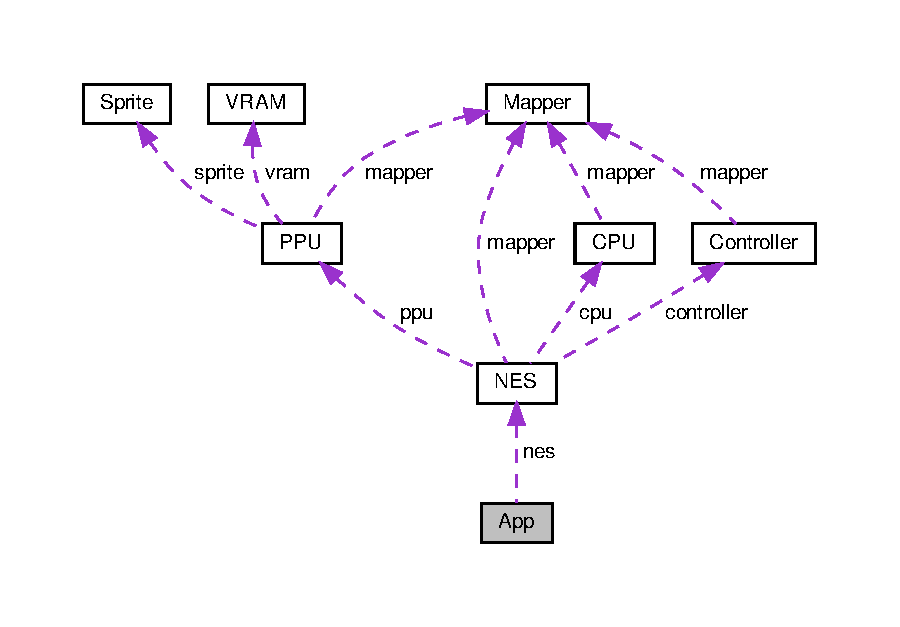
\includegraphics[width=350pt]{struct_app__coll__graph}
\end{center}
\end{figure}
\subsection*{Data Fields}
\begin{DoxyCompactItemize}
\item 
\hyperlink{struct_n_e_s}{N\+ES} $\ast$ \hyperlink{struct_app_ad114e77101488c8e1bcc3a9dec07a54a}{nes}
\item 
S\+D\+L\+\_\+\+Surface $\ast$ \hyperlink{struct_app_a78fa3957d73de49cb81d047857504218}{screen}
\item 
uint16\+\_\+t \hyperlink{struct_app_ae6ca1436ec0a9fd20c44b9a789f748dd}{keys\+Config} \mbox{[}16\mbox{]}
\item 
uint8\+\_\+t \hyperlink{struct_app_a616c0a72f0e4af38b93c736773ac7210}{scale}
\item 
uint32\+\_\+t \hyperlink{struct_app_a08de9232616eaf6a59a7cf46e2b5f437}{next\+Flip}
\end{DoxyCompactItemize}


\subsection{Detailed Description}
Hold application data. 

\subsection{Field Documentation}
\mbox{\Hypertarget{struct_app_ae6ca1436ec0a9fd20c44b9a789f748dd}\label{struct_app_ae6ca1436ec0a9fd20c44b9a789f748dd}} 
\index{App@{App}!keys\+Config@{keys\+Config}}
\index{keys\+Config@{keys\+Config}!App@{App}}
\subsubsection{\texorpdfstring{keys\+Config}{keysConfig}}
{\footnotesize\ttfamily uint16\+\_\+t keys\+Config\mbox{[}16\mbox{]}}

Key configuration \mbox{\Hypertarget{struct_app_ad114e77101488c8e1bcc3a9dec07a54a}\label{struct_app_ad114e77101488c8e1bcc3a9dec07a54a}} 
\index{App@{App}!nes@{nes}}
\index{nes@{nes}!App@{App}}
\subsubsection{\texorpdfstring{nes}{nes}}
{\footnotesize\ttfamily \hyperlink{struct_n_e_s}{N\+ES}$\ast$ nes}

Instance of \hyperlink{struct_n_e_s}{N\+ES} emulator \mbox{\Hypertarget{struct_app_a08de9232616eaf6a59a7cf46e2b5f437}\label{struct_app_a08de9232616eaf6a59a7cf46e2b5f437}} 
\index{App@{App}!next\+Flip@{next\+Flip}}
\index{next\+Flip@{next\+Flip}!App@{App}}
\subsubsection{\texorpdfstring{next\+Flip}{nextFlip}}
{\footnotesize\ttfamily uint32\+\_\+t next\+Flip}

Timestamp to next frame \mbox{\Hypertarget{struct_app_a616c0a72f0e4af38b93c736773ac7210}\label{struct_app_a616c0a72f0e4af38b93c736773ac7210}} 
\index{App@{App}!scale@{scale}}
\index{scale@{scale}!App@{App}}
\subsubsection{\texorpdfstring{scale}{scale}}
{\footnotesize\ttfamily uint8\+\_\+t scale}

Scale factor for rendering \mbox{\Hypertarget{struct_app_a78fa3957d73de49cb81d047857504218}\label{struct_app_a78fa3957d73de49cb81d047857504218}} 
\index{App@{App}!screen@{screen}}
\index{screen@{screen}!App@{App}}
\subsubsection{\texorpdfstring{screen}{screen}}
{\footnotesize\ttfamily S\+D\+L\+\_\+\+Surface$\ast$ screen}

Main screen surface 

The documentation for this struct was generated from the following file\+:\begin{DoxyCompactItemize}
\item 
src/\hyperlink{app_8h}{app.\+h}\end{DoxyCompactItemize}

\hypertarget{struct_controller}{}\section{Controller Struct Reference}
\label{struct_controller}\index{Controller@{Controller}}


Holds necessary variables for the controller emulation to work. Only support the standard joypads.  




{\ttfamily \#include $<$controller.\+h$>$}



Collaboration diagram for Controller\+:\nopagebreak
\begin{figure}[H]
\begin{center}
\leavevmode
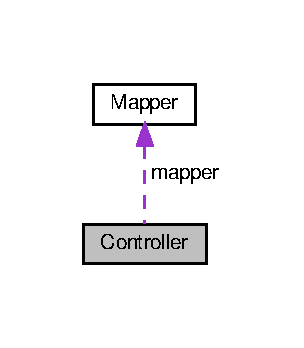
\includegraphics[width=146pt]{struct_controller__coll__graph}
\end{center}
\end{figure}
\subsection*{Data Fields}
\begin{DoxyCompactItemize}
\item 
\mbox{\Hypertarget{struct_controller_a7c8d04b2a02a38530a7bbb870be9f094}\label{struct_controller_a7c8d04b2a02a38530a7bbb870be9f094}} 
int {\bfseries last\+State}
\item 
\mbox{\Hypertarget{struct_controller_aa19f89fe7163aff8f62b6e4436e8cca1}\label{struct_controller_aa19f89fe7163aff8f62b6e4436e8cca1}} 
int {\bfseries shift\+State}
\item 
\mbox{\Hypertarget{struct_controller_a4eded182e423bbc78b60656212249e42}\label{struct_controller_a4eded182e423bbc78b60656212249e42}} 
int {\bfseries polling}
\item 
\mbox{\Hypertarget{struct_controller_a491d7829583d7ed7aa1e18ec246366e2}\label{struct_controller_a491d7829583d7ed7aa1e18ec246366e2}} 
uint16\+\_\+t {\bfseries keys}
\item 
\mbox{\Hypertarget{struct_controller_a2a9230344a369ccd1d395edd03dd6827}\label{struct_controller_a2a9230344a369ccd1d395edd03dd6827}} 
\hyperlink{struct_mapper}{Mapper} $\ast$ {\bfseries mapper}
\item 
\mbox{\Hypertarget{struct_controller_a6fab29dc7e4f8b40ebb1accd52237a4a}\label{struct_controller_a6fab29dc7e4f8b40ebb1accd52237a4a}} 
uint8\+\_\+t {\bfseries J\+O\+Y1}
\item 
\mbox{\Hypertarget{struct_controller_a4b143bcfc6b5049d4cbf8af325d4997a}\label{struct_controller_a4b143bcfc6b5049d4cbf8af325d4997a}} 
uint8\+\_\+t {\bfseries J\+O\+Y2}
\end{DoxyCompactItemize}


\subsection{Detailed Description}
Holds necessary variables for the controller emulation to work. Only support the standard joypads. 

The documentation for this struct was generated from the following file\+:\begin{DoxyCompactItemize}
\item 
src/nes/controller/\hyperlink{controller_8h}{controller.\+h}\end{DoxyCompactItemize}

\hypertarget{struct_c_p_u}{}\section{C\+PU Struct Reference}
\label{struct_c_p_u}\index{C\+PU@{C\+PU}}


Hold \hyperlink{struct_c_p_u}{C\+PU}\textquotesingle{}s register and memory.  




{\ttfamily \#include $<$cpu.\+h$>$}



Collaboration diagram for C\+PU\+:\nopagebreak
\begin{figure}[H]
\begin{center}
\leavevmode
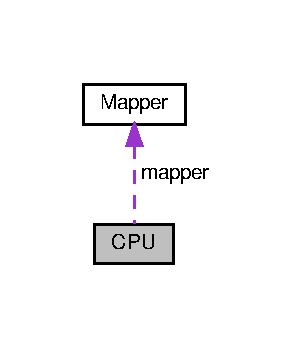
\includegraphics[width=141pt]{struct_c_p_u__coll__graph}
\end{center}
\end{figure}
\subsection*{Data Fields}
\begin{DoxyCompactItemize}
\item 
uint8\+\_\+t \hyperlink{struct_c_p_u_a82fee18d426d3096d23e36cf11ee1995}{O\+A\+M\+D\+MA}
\item 
uint8\+\_\+t \hyperlink{struct_c_p_u_aa99de428bd3e7715b73b335a5af9e900}{A}
\item 
uint8\+\_\+t \hyperlink{struct_c_p_u_aab1bda195b91ffec73b84bc55e9dccf1}{X}
\item 
uint8\+\_\+t \hyperlink{struct_c_p_u_a76ad371f34c724bc71c518bd836a2e2b}{Y}
\item 
uint8\+\_\+t \hyperlink{struct_c_p_u_a11a50c8ce97cdc9e1588fa7201e388f3}{SP}
\item 
uint8\+\_\+t \hyperlink{struct_c_p_u_a2ad95e9194a5bfaa373bbd26ea925209}{P}
\item 
uint16\+\_\+t \hyperlink{struct_c_p_u_afa06037aaac5044b97dde7b9f8771ce6}{PC}
\item 
int16\+\_\+t \hyperlink{struct_c_p_u_a5e42ea87358490e9b0240807c963a734}{cnt\+D\+MA}
\item 
\hyperlink{struct_mapper}{Mapper} $\ast$ \hyperlink{struct_c_p_u_a2a9230344a369ccd1d395edd03dd6827}{mapper}
\end{DoxyCompactItemize}


\subsection{Detailed Description}
Hold \hyperlink{struct_c_p_u}{C\+PU}\textquotesingle{}s register and memory. 

\subsection{Field Documentation}
\mbox{\Hypertarget{struct_c_p_u_aa99de428bd3e7715b73b335a5af9e900}\label{struct_c_p_u_aa99de428bd3e7715b73b335a5af9e900}} 
\index{C\+PU@{C\+PU}!A@{A}}
\index{A@{A}!C\+PU@{C\+PU}}
\subsubsection{\texorpdfstring{A}{A}}
{\footnotesize\ttfamily uint8\+\_\+t A}

Accumulator \mbox{\Hypertarget{struct_c_p_u_a5e42ea87358490e9b0240807c963a734}\label{struct_c_p_u_a5e42ea87358490e9b0240807c963a734}} 
\index{C\+PU@{C\+PU}!cnt\+D\+MA@{cnt\+D\+MA}}
\index{cnt\+D\+MA@{cnt\+D\+MA}!C\+PU@{C\+PU}}
\subsubsection{\texorpdfstring{cnt\+D\+MA}{cntDMA}}
{\footnotesize\ttfamily int16\+\_\+t cnt\+D\+MA}

D\+MA counter \mbox{\Hypertarget{struct_c_p_u_a2a9230344a369ccd1d395edd03dd6827}\label{struct_c_p_u_a2a9230344a369ccd1d395edd03dd6827}} 
\index{C\+PU@{C\+PU}!mapper@{mapper}}
\index{mapper@{mapper}!C\+PU@{C\+PU}}
\subsubsection{\texorpdfstring{mapper}{mapper}}
{\footnotesize\ttfamily \hyperlink{struct_mapper}{Mapper}$\ast$ mapper}

\hyperlink{struct_mapper}{Mapper} to get data from \mbox{\Hypertarget{struct_c_p_u_a82fee18d426d3096d23e36cf11ee1995}\label{struct_c_p_u_a82fee18d426d3096d23e36cf11ee1995}} 
\index{C\+PU@{C\+PU}!O\+A\+M\+D\+MA@{O\+A\+M\+D\+MA}}
\index{O\+A\+M\+D\+MA@{O\+A\+M\+D\+MA}!C\+PU@{C\+PU}}
\subsubsection{\texorpdfstring{O\+A\+M\+D\+MA}{OAMDMA}}
{\footnotesize\ttfamily uint8\+\_\+t O\+A\+M\+D\+MA}

\hyperlink{struct_c_p_u}{C\+PU} address to copy 256 bytes to O\+AM \mbox{\Hypertarget{struct_c_p_u_a2ad95e9194a5bfaa373bbd26ea925209}\label{struct_c_p_u_a2ad95e9194a5bfaa373bbd26ea925209}} 
\index{C\+PU@{C\+PU}!P@{P}}
\index{P@{P}!C\+PU@{C\+PU}}
\subsubsection{\texorpdfstring{P}{P}}
{\footnotesize\ttfamily uint8\+\_\+t P}

Status \mbox{\Hypertarget{struct_c_p_u_afa06037aaac5044b97dde7b9f8771ce6}\label{struct_c_p_u_afa06037aaac5044b97dde7b9f8771ce6}} 
\index{C\+PU@{C\+PU}!PC@{PC}}
\index{PC@{PC}!C\+PU@{C\+PU}}
\subsubsection{\texorpdfstring{PC}{PC}}
{\footnotesize\ttfamily uint16\+\_\+t PC}

Program counter \mbox{\Hypertarget{struct_c_p_u_a11a50c8ce97cdc9e1588fa7201e388f3}\label{struct_c_p_u_a11a50c8ce97cdc9e1588fa7201e388f3}} 
\index{C\+PU@{C\+PU}!SP@{SP}}
\index{SP@{SP}!C\+PU@{C\+PU}}
\subsubsection{\texorpdfstring{SP}{SP}}
{\footnotesize\ttfamily uint8\+\_\+t SP}

\hyperlink{struct_stack}{Stack} Pointer \mbox{\Hypertarget{struct_c_p_u_aab1bda195b91ffec73b84bc55e9dccf1}\label{struct_c_p_u_aab1bda195b91ffec73b84bc55e9dccf1}} 
\index{C\+PU@{C\+PU}!X@{X}}
\index{X@{X}!C\+PU@{C\+PU}}
\subsubsection{\texorpdfstring{X}{X}}
{\footnotesize\ttfamily uint8\+\_\+t X}

X index \mbox{\Hypertarget{struct_c_p_u_a76ad371f34c724bc71c518bd836a2e2b}\label{struct_c_p_u_a76ad371f34c724bc71c518bd836a2e2b}} 
\index{C\+PU@{C\+PU}!Y@{Y}}
\index{Y@{Y}!C\+PU@{C\+PU}}
\subsubsection{\texorpdfstring{Y}{Y}}
{\footnotesize\ttfamily uint8\+\_\+t Y}

Y index 

The documentation for this struct was generated from the following file\+:\begin{DoxyCompactItemize}
\item 
src/nes/cpu/\hyperlink{cpu_8h}{cpu.\+h}\end{DoxyCompactItemize}

\hypertarget{struct_header}{}\section{Header Struct Reference}
\label{struct_header}\index{Header@{Header}}


\hyperlink{struct_header}{Header} of a .nes file, modified for programming purposes.  




{\ttfamily \#include $<$loader.\+h$>$}

\subsection*{Data Fields}
\begin{DoxyCompactItemize}
\item 
uint8\+\_\+t \hyperlink{struct_header_abc17b83f6b13b83428472dfa9221bfb5}{rom\+Size}
\item 
uint8\+\_\+t \hyperlink{struct_header_a10decd110cedd575129373467ebbb23a}{vrom\+Size}
\item 
uint8\+\_\+t \hyperlink{struct_header_a31d9b2a2cceaa5d61eb13f86a040d3ab}{ram\+Size}
\item 
uint8\+\_\+t \hyperlink{struct_header_a0c8e7d5749b619a9832dc135d4661a72}{mapper}
\item 
uint8\+\_\+t \hyperlink{struct_header_ac46680d85e5d1611f934f355080f0375}{mirroring}
\item 
uint8\+\_\+t \hyperlink{struct_header_a46831b0a31a6ac3731c607dc3696f3e8}{battery\+\_\+backed\+\_\+\+R\+AM}
\item 
uint8\+\_\+t \hyperlink{struct_header_a8038f4af17204ad75f2790932777abea}{trainer}
\item 
uint8\+\_\+t \hyperlink{struct_header_a5183c0eb38d0f53f6e8a9c57bf3fe6fd}{four\+\_\+screen\+\_\+\+V\+R\+AM}
\item 
uint8\+\_\+t \hyperlink{struct_header_a23f751e0854a728c81d30b364ed95366}{V\+S\+\_\+\+System}
\item 
uint8\+\_\+t \hyperlink{struct_header_af63447dae4fa0b3b191c17e93d4b8308}{playchoice}
\item 
uint8\+\_\+t \hyperlink{struct_header_a61db4097a2c0c337f74b4b78af94b3bc}{tv\+System}
\end{DoxyCompactItemize}


\subsection{Detailed Description}
\hyperlink{struct_header}{Header} of a .nes file, modified for programming purposes. 

\subsection{Field Documentation}
\mbox{\Hypertarget{struct_header_a46831b0a31a6ac3731c607dc3696f3e8}\label{struct_header_a46831b0a31a6ac3731c607dc3696f3e8}} 
\index{Header@{Header}!battery\+\_\+backed\+\_\+\+R\+AM@{battery\+\_\+backed\+\_\+\+R\+AM}}
\index{battery\+\_\+backed\+\_\+\+R\+AM@{battery\+\_\+backed\+\_\+\+R\+AM}!Header@{Header}}
\subsubsection{\texorpdfstring{battery\+\_\+backed\+\_\+\+R\+AM}{battery\_backed\_RAM}}
{\footnotesize\ttfamily uint8\+\_\+t battery\+\_\+backed\+\_\+\+R\+AM}

1=Batter-\/backed R\+AM at \$6000-\/\$7\+F\+FF or other persistent memory \mbox{\Hypertarget{struct_header_a5183c0eb38d0f53f6e8a9c57bf3fe6fd}\label{struct_header_a5183c0eb38d0f53f6e8a9c57bf3fe6fd}} 
\index{Header@{Header}!four\+\_\+screen\+\_\+\+V\+R\+AM@{four\+\_\+screen\+\_\+\+V\+R\+AM}}
\index{four\+\_\+screen\+\_\+\+V\+R\+AM@{four\+\_\+screen\+\_\+\+V\+R\+AM}!Header@{Header}}
\subsubsection{\texorpdfstring{four\+\_\+screen\+\_\+\+V\+R\+AM}{four\_screen\_VRAM}}
{\footnotesize\ttfamily uint8\+\_\+t four\+\_\+screen\+\_\+\+V\+R\+AM}

1=Hard-\/wired Four-\/screen \hyperlink{struct_v_r_a_m}{V\+R\+AM} layout \mbox{\Hypertarget{struct_header_a0c8e7d5749b619a9832dc135d4661a72}\label{struct_header_a0c8e7d5749b619a9832dc135d4661a72}} 
\index{Header@{Header}!mapper@{mapper}}
\index{mapper@{mapper}!Header@{Header}}
\subsubsection{\texorpdfstring{mapper}{mapper}}
{\footnotesize\ttfamily uint8\+\_\+t mapper}

i\+N\+ES 1.\+0 mapper number \mbox{\Hypertarget{struct_header_ac46680d85e5d1611f934f355080f0375}\label{struct_header_ac46680d85e5d1611f934f355080f0375}} 
\index{Header@{Header}!mirroring@{mirroring}}
\index{mirroring@{mirroring}!Header@{Header}}
\subsubsection{\texorpdfstring{mirroring}{mirroring}}
{\footnotesize\ttfamily uint8\+\_\+t mirroring}

1=Vertical mirroring, 0=Horizontal or mapper-\/controlled mirroring \mbox{\Hypertarget{struct_header_af63447dae4fa0b3b191c17e93d4b8308}\label{struct_header_af63447dae4fa0b3b191c17e93d4b8308}} 
\index{Header@{Header}!playchoice@{playchoice}}
\index{playchoice@{playchoice}!Header@{Header}}
\subsubsection{\texorpdfstring{playchoice}{playchoice}}
{\footnotesize\ttfamily uint8\+\_\+t playchoice}

1=Playchoice-\/10 bit, Not official \mbox{\Hypertarget{struct_header_a31d9b2a2cceaa5d61eb13f86a040d3ab}\label{struct_header_a31d9b2a2cceaa5d61eb13f86a040d3ab}} 
\index{Header@{Header}!ram\+Size@{ram\+Size}}
\index{ram\+Size@{ram\+Size}!Header@{Header}}
\subsubsection{\texorpdfstring{ram\+Size}{ramSize}}
{\footnotesize\ttfamily uint8\+\_\+t ram\+Size}

Size of P\+RG R\+AM, in 8 kB units \mbox{\Hypertarget{struct_header_abc17b83f6b13b83428472dfa9221bfb5}\label{struct_header_abc17b83f6b13b83428472dfa9221bfb5}} 
\index{Header@{Header}!rom\+Size@{rom\+Size}}
\index{rom\+Size@{rom\+Size}!Header@{Header}}
\subsubsection{\texorpdfstring{rom\+Size}{romSize}}
{\footnotesize\ttfamily uint8\+\_\+t rom\+Size}

Number of 16 kB R\+OM (P\+R\+G-\/\+R\+OM) banks \mbox{\Hypertarget{struct_header_a8038f4af17204ad75f2790932777abea}\label{struct_header_a8038f4af17204ad75f2790932777abea}} 
\index{Header@{Header}!trainer@{trainer}}
\index{trainer@{trainer}!Header@{Header}}
\subsubsection{\texorpdfstring{trainer}{trainer}}
{\footnotesize\ttfamily uint8\+\_\+t trainer}

1=512-\/\+Byte trainer at \$7000-\/\$71\+FF \mbox{\Hypertarget{struct_header_a61db4097a2c0c337f74b4b78af94b3bc}\label{struct_header_a61db4097a2c0c337f74b4b78af94b3bc}} 
\index{Header@{Header}!tv\+System@{tv\+System}}
\index{tv\+System@{tv\+System}!Header@{Header}}
\subsubsection{\texorpdfstring{tv\+System}{tvSystem}}
{\footnotesize\ttfamily uint8\+\_\+t tv\+System}

0=P\+AL, 1=N\+S\+TC \mbox{\Hypertarget{struct_header_a10decd110cedd575129373467ebbb23a}\label{struct_header_a10decd110cedd575129373467ebbb23a}} 
\index{Header@{Header}!vrom\+Size@{vrom\+Size}}
\index{vrom\+Size@{vrom\+Size}!Header@{Header}}
\subsubsection{\texorpdfstring{vrom\+Size}{vromSize}}
{\footnotesize\ttfamily uint8\+\_\+t vrom\+Size}

Number of 8 kB V\+R\+OM (C\+H\+R-\/\+R\+OM) banks \mbox{\Hypertarget{struct_header_a23f751e0854a728c81d30b364ed95366}\label{struct_header_a23f751e0854a728c81d30b364ed95366}} 
\index{Header@{Header}!V\+S\+\_\+\+System@{V\+S\+\_\+\+System}}
\index{V\+S\+\_\+\+System@{V\+S\+\_\+\+System}!Header@{Header}}
\subsubsection{\texorpdfstring{V\+S\+\_\+\+System}{VS\_System}}
{\footnotesize\ttfamily uint8\+\_\+t V\+S\+\_\+\+System}

1=V\+S-\/\+System cartridges 

The documentation for this struct was generated from the following file\+:\begin{DoxyCompactItemize}
\item 
src/nes/loader/\hyperlink{loader_8h}{loader.\+h}\end{DoxyCompactItemize}

\hypertarget{struct_instruction}{}\section{Instruction Struct Reference}
\label{struct_instruction}\index{Instruction@{Instruction}}


Hold \hyperlink{struct_opcode}{Opcode} and arguments associated.  




{\ttfamily \#include $<$instruction.\+h$>$}



Collaboration diagram for Instruction\+:\nopagebreak
\begin{figure}[H]
\begin{center}
\leavevmode
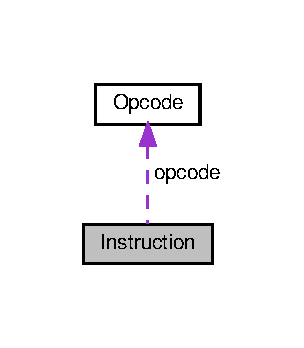
\includegraphics[width=146pt]{struct_instruction__coll__graph}
\end{center}
\end{figure}
\subsection*{Data Fields}
\begin{DoxyCompactItemize}
\item 
\hyperlink{struct_opcode}{Opcode} \hyperlink{struct_instruction_a4ee0311d643454fcf8d4f707fba72a6d}{opcode}
\item 
uint8\+\_\+t \hyperlink{struct_instruction_a59180d12e1d75e81d606a437f3abb293}{opcode\+Arg} \mbox{[}2\mbox{]}
\item 
uint8\+\_\+t $\ast$ \hyperlink{struct_instruction_a42066ad070971025cb7f59390afe49a5}{data\+Mem}
\item 
uint16\+\_\+t \hyperlink{struct_instruction_a88c67627f4474a4fbe6ccabcd34521ae}{data\+Addr}
\item 
uint8\+\_\+t \hyperlink{struct_instruction_a6d48ff193a5218fe9f4089254160f19c}{page\+Crossed}
\item 
uint16\+\_\+t \hyperlink{struct_instruction_a6e22f1a0885905391e81ecf7d78ecf35}{last\+PC}
\item 
uint8\+\_\+t \hyperlink{struct_instruction_a62e2f27f9942405e7def81df4c2b664f}{raw\+Opcode}
\item 
uint8\+\_\+t \hyperlink{struct_instruction_a61f9076307ef1f322f6af2e1b1adea55}{nb\+Arg}
\end{DoxyCompactItemize}


\subsection{Detailed Description}
Hold \hyperlink{struct_opcode}{Opcode} and arguments associated. 

\subsection{Field Documentation}
\mbox{\Hypertarget{struct_instruction_a88c67627f4474a4fbe6ccabcd34521ae}\label{struct_instruction_a88c67627f4474a4fbe6ccabcd34521ae}} 
\index{Instruction@{Instruction}!data\+Addr@{data\+Addr}}
\index{data\+Addr@{data\+Addr}!Instruction@{Instruction}}
\subsubsection{\texorpdfstring{data\+Addr}{dataAddr}}
{\footnotesize\ttfamily uint16\+\_\+t data\+Addr}

Origin of data\+Mem \mbox{\Hypertarget{struct_instruction_a42066ad070971025cb7f59390afe49a5}\label{struct_instruction_a42066ad070971025cb7f59390afe49a5}} 
\index{Instruction@{Instruction}!data\+Mem@{data\+Mem}}
\index{data\+Mem@{data\+Mem}!Instruction@{Instruction}}
\subsubsection{\texorpdfstring{data\+Mem}{dataMem}}
{\footnotesize\ttfamily uint8\+\_\+t$\ast$ data\+Mem}

Pointer to data to work with \mbox{\Hypertarget{struct_instruction_a6e22f1a0885905391e81ecf7d78ecf35}\label{struct_instruction_a6e22f1a0885905391e81ecf7d78ecf35}} 
\index{Instruction@{Instruction}!last\+PC@{last\+PC}}
\index{last\+PC@{last\+PC}!Instruction@{Instruction}}
\subsubsection{\texorpdfstring{last\+PC}{lastPC}}
{\footnotesize\ttfamily uint16\+\_\+t last\+PC}

Program counter when decoding \mbox{\Hypertarget{struct_instruction_a61f9076307ef1f322f6af2e1b1adea55}\label{struct_instruction_a61f9076307ef1f322f6af2e1b1adea55}} 
\index{Instruction@{Instruction}!nb\+Arg@{nb\+Arg}}
\index{nb\+Arg@{nb\+Arg}!Instruction@{Instruction}}
\subsubsection{\texorpdfstring{nb\+Arg}{nbArg}}
{\footnotesize\ttfamily uint8\+\_\+t nb\+Arg}

Number of argument given \mbox{\Hypertarget{struct_instruction_a4ee0311d643454fcf8d4f707fba72a6d}\label{struct_instruction_a4ee0311d643454fcf8d4f707fba72a6d}} 
\index{Instruction@{Instruction}!opcode@{opcode}}
\index{opcode@{opcode}!Instruction@{Instruction}}
\subsubsection{\texorpdfstring{opcode}{opcode}}
{\footnotesize\ttfamily \hyperlink{struct_opcode}{Opcode} opcode}

\hyperlink{struct_opcode}{Opcode} information \mbox{\Hypertarget{struct_instruction_a59180d12e1d75e81d606a437f3abb293}\label{struct_instruction_a59180d12e1d75e81d606a437f3abb293}} 
\index{Instruction@{Instruction}!opcode\+Arg@{opcode\+Arg}}
\index{opcode\+Arg@{opcode\+Arg}!Instruction@{Instruction}}
\subsubsection{\texorpdfstring{opcode\+Arg}{opcodeArg}}
{\footnotesize\ttfamily uint8\+\_\+t opcode\+Arg\mbox{[}2\mbox{]}}

Argument given with opcode \mbox{\Hypertarget{struct_instruction_a6d48ff193a5218fe9f4089254160f19c}\label{struct_instruction_a6d48ff193a5218fe9f4089254160f19c}} 
\index{Instruction@{Instruction}!page\+Crossed@{page\+Crossed}}
\index{page\+Crossed@{page\+Crossed}!Instruction@{Instruction}}
\subsubsection{\texorpdfstring{page\+Crossed}{pageCrossed}}
{\footnotesize\ttfamily uint8\+\_\+t page\+Crossed}

Page crossed flag \mbox{\Hypertarget{struct_instruction_a62e2f27f9942405e7def81df4c2b664f}\label{struct_instruction_a62e2f27f9942405e7def81df4c2b664f}} 
\index{Instruction@{Instruction}!raw\+Opcode@{raw\+Opcode}}
\index{raw\+Opcode@{raw\+Opcode}!Instruction@{Instruction}}
\subsubsection{\texorpdfstring{raw\+Opcode}{rawOpcode}}
{\footnotesize\ttfamily uint8\+\_\+t raw\+Opcode}

\hyperlink{struct_opcode}{Opcode} byte value 

The documentation for this struct was generated from the following file\+:\begin{DoxyCompactItemize}
\item 
src/nes/cpu/\hyperlink{instruction_8h}{instruction.\+h}\end{DoxyCompactItemize}

\hypertarget{struct_i_o_reg}{}\section{I\+O\+Reg Struct Reference}
\label{struct_i_o_reg}\index{I\+O\+Reg@{I\+O\+Reg}}


Register use to communicate with \hyperlink{struct_p_p_u}{P\+PU}, A\+PU and joystick.  




{\ttfamily \#include $<$ioreg.\+h$>$}

\subsection*{Data Fields}
\begin{DoxyCompactItemize}
\item 
uint8\+\_\+t $\ast$ \hyperlink{struct_i_o_reg_a3a254f17251e937f76932c5081eab405}{bank1} \mbox{[}8\mbox{]}
\item 
uint8\+\_\+t $\ast$ \hyperlink{struct_i_o_reg_ae4edb3d07789e7300d9f7ff80927814a}{bank2} \mbox{[}32\mbox{]}
\item 
uint8\+\_\+t \hyperlink{struct_i_o_reg_a33f1fe95e68d8c8ce672496d8d2f9db3}{acknowledge} \mbox{[}40\mbox{]}
\item 
uint8\+\_\+t \hyperlink{struct_i_o_reg_aff7b59f569ec689a7580bd6911daafd5}{dummy}
\end{DoxyCompactItemize}


\subsection{Detailed Description}
Register use to communicate with \hyperlink{struct_p_p_u}{P\+PU}, A\+PU and joystick. 

The structure is composed of two arrays that represent bank in memory map \+:
\begin{DoxyItemize}
\item bank1 \+: @0x2000, registers for \hyperlink{struct_p_p_u}{P\+PU}
\item bank2 \+: @0x4000, registers for A\+PU and joystick Flags array are used to know if data was read or written 
\end{DoxyItemize}

\subsection{Field Documentation}
\mbox{\Hypertarget{struct_i_o_reg_a33f1fe95e68d8c8ce672496d8d2f9db3}\label{struct_i_o_reg_a33f1fe95e68d8c8ce672496d8d2f9db3}} 
\index{I\+O\+Reg@{I\+O\+Reg}!acknowledge@{acknowledge}}
\index{acknowledge@{acknowledge}!I\+O\+Reg@{I\+O\+Reg}}
\subsubsection{\texorpdfstring{acknowledge}{acknowledge}}
{\footnotesize\ttfamily uint8\+\_\+t acknowledge\mbox{[}40\mbox{]}}

Acknowledge array \mbox{\Hypertarget{struct_i_o_reg_a3a254f17251e937f76932c5081eab405}\label{struct_i_o_reg_a3a254f17251e937f76932c5081eab405}} 
\index{I\+O\+Reg@{I\+O\+Reg}!bank1@{bank1}}
\index{bank1@{bank1}!I\+O\+Reg@{I\+O\+Reg}}
\subsubsection{\texorpdfstring{bank1}{bank1}}
{\footnotesize\ttfamily uint8\+\_\+t$\ast$ bank1\mbox{[}8\mbox{]}}

Pointer bank 1 \mbox{\Hypertarget{struct_i_o_reg_ae4edb3d07789e7300d9f7ff80927814a}\label{struct_i_o_reg_ae4edb3d07789e7300d9f7ff80927814a}} 
\index{I\+O\+Reg@{I\+O\+Reg}!bank2@{bank2}}
\index{bank2@{bank2}!I\+O\+Reg@{I\+O\+Reg}}
\subsubsection{\texorpdfstring{bank2}{bank2}}
{\footnotesize\ttfamily uint8\+\_\+t$\ast$ bank2\mbox{[}32\mbox{]}}

Pointer bank 2 \mbox{\Hypertarget{struct_i_o_reg_aff7b59f569ec689a7580bd6911daafd5}\label{struct_i_o_reg_aff7b59f569ec689a7580bd6911daafd5}} 
\index{I\+O\+Reg@{I\+O\+Reg}!dummy@{dummy}}
\index{dummy@{dummy}!I\+O\+Reg@{I\+O\+Reg}}
\subsubsection{\texorpdfstring{dummy}{dummy}}
{\footnotesize\ttfamily uint8\+\_\+t dummy}

Dummy byte which pointer is returned from I\+O\+Reg\+\_\+\+Get for unconnected registers 

The documentation for this struct was generated from the following file\+:\begin{DoxyCompactItemize}
\item 
src/nes/mapper/\hyperlink{ioreg_8h}{ioreg.\+h}\end{DoxyCompactItemize}

\hypertarget{struct_keys}{}\section{Keys Struct Reference}
\label{struct_keys}\index{Keys@{Keys}}


Hold string for key name and corresponding S\+D\+LK constant.  




{\ttfamily \#include $<$keys.\+h$>$}

\subsection*{Data Fields}
\begin{DoxyCompactItemize}
\item 
\mbox{\Hypertarget{struct_keys_ab79a3ac2679b3523c1f53040e820052b}\label{struct_keys_ab79a3ac2679b3523c1f53040e820052b}} 
char $\ast$ {\bfseries key\+Name}
\item 
\mbox{\Hypertarget{struct_keys_a9c6ac273bb07ac0d6dd7cd4c66dfd0ed}\label{struct_keys_a9c6ac273bb07ac0d6dd7cd4c66dfd0ed}} 
int {\bfseries S\+D\+LK}
\end{DoxyCompactItemize}


\subsection{Detailed Description}
Hold string for key name and corresponding S\+D\+LK constant. 

The documentation for this struct was generated from the following file\+:\begin{DoxyCompactItemize}
\item 
src/common/\hyperlink{keys_8h}{keys.\+h}\end{DoxyCompactItemize}

\hypertarget{struct_map_n_r_o_m}{}\section{Map\+N\+R\+OM Struct Reference}
\label{struct_map_n_r_o_m}\index{Map\+N\+R\+OM@{Map\+N\+R\+OM}}


Memory map used when using N\+R\+OM mapper.  




{\ttfamily \#include $<$nrom.\+h$>$}



Collaboration diagram for Map\+N\+R\+OM\+:\nopagebreak
\begin{figure}[H]
\begin{center}
\leavevmode
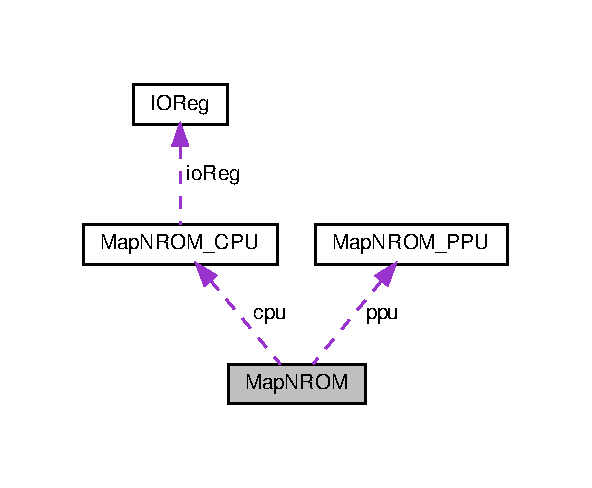
\includegraphics[width=284pt]{struct_map_n_r_o_m__coll__graph}
\end{center}
\end{figure}
\subsection*{Data Fields}
\begin{DoxyCompactItemize}
\item 
\mbox{\Hypertarget{struct_map_n_r_o_m_ab87ce31650d5ba5e7e2b656779561256}\label{struct_map_n_r_o_m_ab87ce31650d5ba5e7e2b656779561256}} 
\hyperlink{struct_map_n_r_o_m___c_p_u}{Map\+N\+R\+O\+M\+\_\+\+C\+PU} {\bfseries cpu}
\item 
\mbox{\Hypertarget{struct_map_n_r_o_m_a01d9d5e915588759aaa5863846887cb2}\label{struct_map_n_r_o_m_a01d9d5e915588759aaa5863846887cb2}} 
\hyperlink{struct_map_n_r_o_m___p_p_u}{Map\+N\+R\+O\+M\+\_\+\+P\+PU} {\bfseries ppu}
\item 
\mbox{\Hypertarget{struct_map_n_r_o_m_aff7b59f569ec689a7580bd6911daafd5}\label{struct_map_n_r_o_m_aff7b59f569ec689a7580bd6911daafd5}} 
uint8\+\_\+t {\bfseries dummy}
\item 
\mbox{\Hypertarget{struct_map_n_r_o_m_abc17b83f6b13b83428472dfa9221bfb5}\label{struct_map_n_r_o_m_abc17b83f6b13b83428472dfa9221bfb5}} 
uint8\+\_\+t {\bfseries rom\+Size}
\item 
\mbox{\Hypertarget{struct_map_n_r_o_m_ac46680d85e5d1611f934f355080f0375}\label{struct_map_n_r_o_m_ac46680d85e5d1611f934f355080f0375}} 
uint8\+\_\+t {\bfseries mirroring}
\end{DoxyCompactItemize}


\subsection{Detailed Description}
Memory map used when using N\+R\+OM mapper. 

The documentation for this struct was generated from the following file\+:\begin{DoxyCompactItemize}
\item 
src/nes/mapper/\hyperlink{nrom_8h}{nrom.\+h}\end{DoxyCompactItemize}

\hypertarget{struct_map_n_r_o_m___c_p_u}{}\section{Map\+N\+R\+O\+M\+\_\+\+C\+PU Struct Reference}
\label{struct_map_n_r_o_m___c_p_u}\index{Map\+N\+R\+O\+M\+\_\+\+C\+PU@{Map\+N\+R\+O\+M\+\_\+\+C\+PU}}


Memory map of \hyperlink{struct_c_p_u}{C\+PU} when using N\+R\+OM mapper.  




{\ttfamily \#include $<$nrom.\+h$>$}



Collaboration diagram for Map\+N\+R\+O\+M\+\_\+\+C\+PU\+:\nopagebreak
\begin{figure}[H]
\begin{center}
\leavevmode
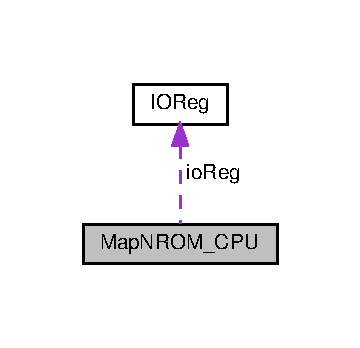
\includegraphics[width=173pt]{struct_map_n_r_o_m___c_p_u__coll__graph}
\end{center}
\end{figure}
\subsection*{Data Fields}
\begin{DoxyCompactItemize}
\item 
\mbox{\Hypertarget{struct_map_n_r_o_m___c_p_u_adab6a729af9f9f093a789113341473de}\label{struct_map_n_r_o_m___c_p_u_adab6a729af9f9f093a789113341473de}} 
uint8\+\_\+t $\ast$ {\bfseries ram}
\item 
\mbox{\Hypertarget{struct_map_n_r_o_m___c_p_u_a8ca82c9835d272c0333147840355f411}\label{struct_map_n_r_o_m___c_p_u_a8ca82c9835d272c0333147840355f411}} 
\hyperlink{struct_i_o_reg}{I\+O\+Reg} $\ast$ {\bfseries io\+Reg}
\item 
\mbox{\Hypertarget{struct_map_n_r_o_m___c_p_u_a089eb276a325916466365816fb314059}\label{struct_map_n_r_o_m___c_p_u_a089eb276a325916466365816fb314059}} 
uint8\+\_\+t $\ast$ {\bfseries sram}
\item 
\mbox{\Hypertarget{struct_map_n_r_o_m___c_p_u_a95644251ecc17b2b3203dd6f34351183}\label{struct_map_n_r_o_m___c_p_u_a95644251ecc17b2b3203dd6f34351183}} 
uint8\+\_\+t $\ast$ {\bfseries rom}
\end{DoxyCompactItemize}


\subsection{Detailed Description}
Memory map of \hyperlink{struct_c_p_u}{C\+PU} when using N\+R\+OM mapper. 

The documentation for this struct was generated from the following file\+:\begin{DoxyCompactItemize}
\item 
src/nes/mapper/\hyperlink{nrom_8h}{nrom.\+h}\end{DoxyCompactItemize}

\hypertarget{struct_map_n_r_o_m___p_p_u}{}\section{Map\+N\+R\+O\+M\+\_\+\+P\+PU Struct Reference}
\label{struct_map_n_r_o_m___p_p_u}\index{Map\+N\+R\+O\+M\+\_\+\+P\+PU@{Map\+N\+R\+O\+M\+\_\+\+P\+PU}}


Memory map of \hyperlink{struct_p_p_u}{P\+PU} when using N\+R\+OM mapper.  




{\ttfamily \#include $<$nrom.\+h$>$}

\subsection*{Data Fields}
\begin{DoxyCompactItemize}
\item 
\mbox{\Hypertarget{struct_map_n_r_o_m___p_p_u_a17b2c8b808feb624a4ba042b1389bcdd}\label{struct_map_n_r_o_m___p_p_u_a17b2c8b808feb624a4ba042b1389bcdd}} 
uint8\+\_\+t $\ast$ {\bfseries chr}
\item 
\mbox{\Hypertarget{struct_map_n_r_o_m___p_p_u_ab200315b5565da275df8d5ed67152b1c}\label{struct_map_n_r_o_m___p_p_u_ab200315b5565da275df8d5ed67152b1c}} 
uint8\+\_\+t $\ast$ {\bfseries nametable}
\item 
\mbox{\Hypertarget{struct_map_n_r_o_m___p_p_u_a8b0a4284623f652d89a87c675d8f81a0}\label{struct_map_n_r_o_m___p_p_u_a8b0a4284623f652d89a87c675d8f81a0}} 
uint8\+\_\+t $\ast$ {\bfseries palette}
\end{DoxyCompactItemize}


\subsection{Detailed Description}
Memory map of \hyperlink{struct_p_p_u}{P\+PU} when using N\+R\+OM mapper. 

The documentation for this struct was generated from the following file\+:\begin{DoxyCompactItemize}
\item 
src/nes/mapper/\hyperlink{nrom_8h}{nrom.\+h}\end{DoxyCompactItemize}

\hypertarget{struct_mapper}{}\section{Mapper Struct Reference}
\label{struct_mapper}\index{Mapper@{Mapper}}


Generic structure to hold mapper.  




{\ttfamily \#include $<$mapper.\+h$>$}

\subsection*{Data Fields}
\begin{DoxyCompactItemize}
\item 
\mbox{\Hypertarget{struct_mapper_a2ec355646dbdcfd7f762b06a233067d5}\label{struct_mapper_a2ec355646dbdcfd7f762b06a233067d5}} 
void $\ast$($\ast$ {\bfseries get} )(void $\ast$, uint8\+\_\+t, uint16\+\_\+t)
\item 
void($\ast$ \hyperlink{struct_mapper_a6d5022ea505e6c2ce03eee79a76c0c49}{destroyer} )(void $\ast$)
\item 
uint8\+\_\+t($\ast$ \hyperlink{struct_mapper_a30f4bc8c14f8ed6b602d081e28e387a5}{ack} )(void $\ast$, uint16\+\_\+t)
\item 
void $\ast$ \hyperlink{struct_mapper_a417be0ec6d49a8fade0fa596656d1d43}{mapper\+Data}
\end{DoxyCompactItemize}


\subsection{Detailed Description}
Generic structure to hold mapper. 

\subsection{Field Documentation}
\mbox{\Hypertarget{struct_mapper_a30f4bc8c14f8ed6b602d081e28e387a5}\label{struct_mapper_a30f4bc8c14f8ed6b602d081e28e387a5}} 
\index{Mapper@{Mapper}!ack@{ack}}
\index{ack@{ack}!Mapper@{Mapper}}
\subsubsection{\texorpdfstring{ack}{ack}}
{\footnotesize\ttfamily uint8\+\_\+t($\ast$ ack) (void $\ast$, uint16\+\_\+t)}

Destroyer callback \mbox{\Hypertarget{struct_mapper_a6d5022ea505e6c2ce03eee79a76c0c49}\label{struct_mapper_a6d5022ea505e6c2ce03eee79a76c0c49}} 
\index{Mapper@{Mapper}!destroyer@{destroyer}}
\index{destroyer@{destroyer}!Mapper@{Mapper}}
\subsubsection{\texorpdfstring{destroyer}{destroyer}}
{\footnotesize\ttfamily void($\ast$ destroyer) (void $\ast$)}

Get callback \mbox{\Hypertarget{struct_mapper_a417be0ec6d49a8fade0fa596656d1d43}\label{struct_mapper_a417be0ec6d49a8fade0fa596656d1d43}} 
\index{Mapper@{Mapper}!mapper\+Data@{mapper\+Data}}
\index{mapper\+Data@{mapper\+Data}!Mapper@{Mapper}}
\subsubsection{\texorpdfstring{mapper\+Data}{mapperData}}
{\footnotesize\ttfamily void$\ast$ mapper\+Data}

Acknowledge callback 

The documentation for this struct was generated from the following file\+:\begin{DoxyCompactItemize}
\item 
src/nes/mapper/\hyperlink{mapper_8h}{mapper.\+h}\end{DoxyCompactItemize}

\hypertarget{struct_n_e_s}{}\section{N\+ES Struct Reference}
\label{struct_n_e_s}\index{N\+ES@{N\+ES}}


Hold every component to emulate the Nintendo Entertainement System.  




{\ttfamily \#include $<$nes.\+h$>$}



Collaboration diagram for N\+ES\+:\nopagebreak
\begin{figure}[H]
\begin{center}
\leavevmode
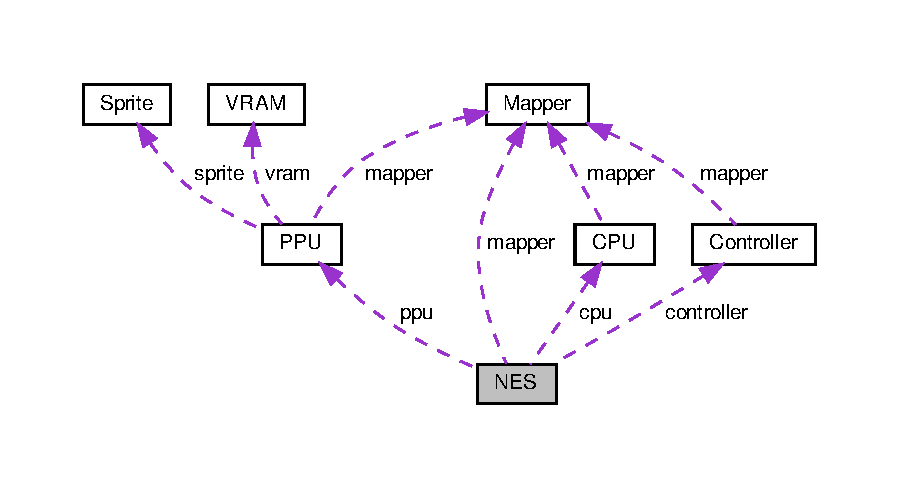
\includegraphics[width=350pt]{struct_n_e_s__coll__graph}
\end{center}
\end{figure}
\subsection*{Data Fields}
\begin{DoxyCompactItemize}
\item 
\mbox{\Hypertarget{struct_n_e_s_a7841e50a9c480edc0df1f395bc792d20}\label{struct_n_e_s_a7841e50a9c480edc0df1f395bc792d20}} 
\hyperlink{struct_c_p_u}{C\+PU} $\ast$ {\bfseries cpu}
\item 
\mbox{\Hypertarget{struct_n_e_s_a19ff22373983c5d02166b6c29f2de187}\label{struct_n_e_s_a19ff22373983c5d02166b6c29f2de187}} 
\hyperlink{struct_p_p_u}{P\+PU} $\ast$ {\bfseries ppu}
\item 
\mbox{\Hypertarget{struct_n_e_s_acaf0644c14bf7a45d314781c4168cb83}\label{struct_n_e_s_acaf0644c14bf7a45d314781c4168cb83}} 
\hyperlink{struct_controller}{Controller} $\ast$ {\bfseries controller}
\item 
\mbox{\Hypertarget{struct_n_e_s_a2a9230344a369ccd1d395edd03dd6827}\label{struct_n_e_s_a2a9230344a369ccd1d395edd03dd6827}} 
\hyperlink{struct_mapper}{Mapper} $\ast$ {\bfseries mapper}
\item 
\mbox{\Hypertarget{struct_n_e_s_abf614a5e77e47c9622abbc45420cb567}\label{struct_n_e_s_abf614a5e77e47c9622abbc45420cb567}} 
uint32\+\_\+t {\bfseries clock\+Count}
\item 
\mbox{\Hypertarget{struct_n_e_s_af3db2773a8619d9a7c7729880f808113}\label{struct_n_e_s_af3db2773a8619d9a7c7729880f808113}} 
uint8\+\_\+t {\bfseries context}
\end{DoxyCompactItemize}


\subsection{Detailed Description}
Hold every component to emulate the Nintendo Entertainement System. 

The documentation for this struct was generated from the following file\+:\begin{DoxyCompactItemize}
\item 
src/nes/\hyperlink{nes_8h}{nes.\+h}\end{DoxyCompactItemize}

\hypertarget{struct_opcode}{}\section{Opcode Struct Reference}
\label{struct_opcode}\index{Opcode@{Opcode}}


Hold instruction function and addressing mode associated.  




{\ttfamily \#include $<$instruction.\+h$>$}

\subsection*{Data Fields}
\begin{DoxyCompactItemize}
\item 
uint8\+\_\+t($\ast$ \hyperlink{struct_opcode_aaac3f46611559561cb0430bdb8d0741d}{inst} )(\hyperlink{struct_c_p_u}{C\+PU} $\ast$, \hyperlink{struct_instruction}{Instruction} $\ast$)
\item 
uint8\+\_\+t \hyperlink{struct_opcode_af769224d4cd14a6d914fe7f7e3c8804f}{addressing\+Mode}
\item 
uint8\+\_\+t \hyperlink{struct_opcode_a43925d437f42c3541f76d1ef391476ca}{cycle}
\end{DoxyCompactItemize}


\subsection{Detailed Description}
Hold instruction function and addressing mode associated. 

\subsection{Field Documentation}
\mbox{\Hypertarget{struct_opcode_af769224d4cd14a6d914fe7f7e3c8804f}\label{struct_opcode_af769224d4cd14a6d914fe7f7e3c8804f}} 
\index{Opcode@{Opcode}!addressing\+Mode@{addressing\+Mode}}
\index{addressing\+Mode@{addressing\+Mode}!Opcode@{Opcode}}
\subsubsection{\texorpdfstring{addressing\+Mode}{addressingMode}}
{\footnotesize\ttfamily uint8\+\_\+t addressing\+Mode}

Addressing mode used \mbox{\Hypertarget{struct_opcode_a43925d437f42c3541f76d1ef391476ca}\label{struct_opcode_a43925d437f42c3541f76d1ef391476ca}} 
\index{Opcode@{Opcode}!cycle@{cycle}}
\index{cycle@{cycle}!Opcode@{Opcode}}
\subsubsection{\texorpdfstring{cycle}{cycle}}
{\footnotesize\ttfamily uint8\+\_\+t cycle}

Cycle consumption \mbox{\Hypertarget{struct_opcode_aaac3f46611559561cb0430bdb8d0741d}\label{struct_opcode_aaac3f46611559561cb0430bdb8d0741d}} 
\index{Opcode@{Opcode}!inst@{inst}}
\index{inst@{inst}!Opcode@{Opcode}}
\subsubsection{\texorpdfstring{inst}{inst}}
{\footnotesize\ttfamily uint8\+\_\+t($\ast$ inst) (\hyperlink{struct_c_p_u}{C\+PU} $\ast$, \hyperlink{struct_instruction}{Instruction} $\ast$)}

\hyperlink{struct_instruction}{Instruction} callback 

The documentation for this struct was generated from the following file\+:\begin{DoxyCompactItemize}
\item 
src/nes/cpu/\hyperlink{instruction_8h}{instruction.\+h}\end{DoxyCompactItemize}

\hypertarget{struct_p_p_u}{}\section{P\+PU Struct Reference}
\label{struct_p_p_u}\index{P\+PU@{P\+PU}}


Hold every variable needed to run \hyperlink{struct_p_p_u}{P\+PU}.  




{\ttfamily \#include $<$ppu.\+h$>$}



Collaboration diagram for P\+PU\+:\nopagebreak
\begin{figure}[H]
\begin{center}
\leavevmode
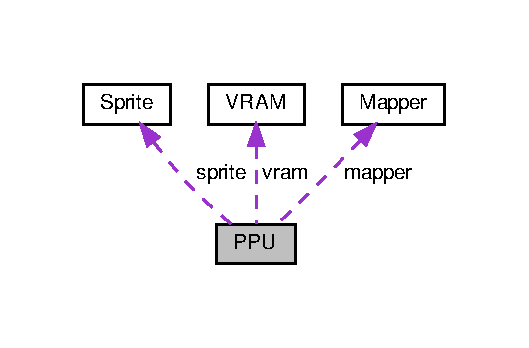
\includegraphics[width=254pt]{struct_p_p_u__coll__graph}
\end{center}
\end{figure}
\subsection*{Data Fields}
\begin{DoxyCompactItemize}
\item 
uint8\+\_\+t \hyperlink{struct_p_p_u_af3b4f665eb5f55ad9b2919464e19c64a}{P\+P\+U\+C\+T\+RL}
\item 
uint8\+\_\+t \hyperlink{struct_p_p_u_a6ec06ed9d7a2fd84300fc764e3e96672}{P\+P\+U\+M\+A\+SK}
\item 
uint8\+\_\+t \hyperlink{struct_p_p_u_a7773485ae6289f9a57d30d4a66458581}{P\+P\+U\+S\+T\+A\+T\+US}
\item 
uint8\+\_\+t \hyperlink{struct_p_p_u_ad52128da7e77b60540403b30502961de}{O\+A\+M\+A\+D\+DR}
\item 
uint8\+\_\+t \hyperlink{struct_p_p_u_a9665053d5b09aed492922e997f29e7ea}{O\+A\+M\+D\+A\+TA}
\item 
uint8\+\_\+t \hyperlink{struct_p_p_u_a192557bebe1fba78011e23552e245f35}{P\+P\+U\+S\+C\+R\+O\+LL}
\item 
uint8\+\_\+t \hyperlink{struct_p_p_u_aa2fbeb7a018d444d942c9998968251a9}{P\+P\+U\+A\+D\+DR}
\item 
uint8\+\_\+t \hyperlink{struct_p_p_u_a21e9356a3ea5f41d1ba6fc9782e953e5}{P\+P\+U\+D\+A\+TA}
\item 
\hyperlink{struct_mapper}{Mapper} $\ast$ \hyperlink{struct_p_p_u_a2a9230344a369ccd1d395edd03dd6827}{mapper}
\item 
\hyperlink{struct_v_r_a_m}{V\+R\+AM} \hyperlink{struct_p_p_u_abc329fd3bb95268164f54c040118ab9c}{vram}
\item 
uint16\+\_\+t \hyperlink{struct_p_p_u_a27eb4db4e065eac424e15c0c6569d1d7}{cycle}
\item 
int16\+\_\+t \hyperlink{struct_p_p_u_aeb74e7c9eef1621e3ffe44360ddbf703}{scanline}
\item 
uint8\+\_\+t \hyperlink{struct_p_p_u_a91e5e30500bc47619f6002b304d4871d}{nb\+Frame}
\item 
uint8\+\_\+t \hyperlink{struct_p_p_u_ab4122702865e26c18ac2bf11ff2db948}{nmi\+Sent}
\item 
uint8\+\_\+t \hyperlink{struct_p_p_u_a5f7a6e84f511fc321dd7206d331d778a}{picture\+Drawn}
\item 
uint8\+\_\+t \hyperlink{struct_p_p_u_a3b60c82c8daf2a08b49d8bda55d7d819}{O\+AM} \mbox{[}256\mbox{]}
\item 
uint8\+\_\+t \hyperlink{struct_p_p_u_a47d494976b32bbdde6b2a0947132686d}{S\+O\+AM} \mbox{[}32\mbox{]}
\item 
uint8\+\_\+t \hyperlink{struct_p_p_u_a496affeb5a831e004a615b888e98e85e}{S\+O\+A\+M\+A\+D\+DR}
\item 
uint8\+\_\+t \hyperlink{struct_p_p_u_a22a6738b7311f8741c18f199215724c6}{sprite\+State}
\item 
uint8\+\_\+t \hyperlink{struct_p_p_u_abf381ae655282a3beee0563e6d6bce75}{sprite\+Data}
\item 
uint8\+\_\+t \hyperlink{struct_p_p_u_ab7fdc3f45d8fd245221d2dd1cca96d7d}{sprite\+Zero}
\item 
uint32\+\_\+t $\ast$ \hyperlink{struct_p_p_u_ac8986adb5b1723b0ee8c6d7b28ab921b}{image}
\item 
uint16\+\_\+t \hyperlink{struct_p_p_u_adc60b544127ab0cf3f48bec16b090fe0}{bitmapL}
\item 
uint16\+\_\+t \hyperlink{struct_p_p_u_a0487b25ddf967f4aca280bca7c67336c}{bitmapH}
\item 
uint16\+\_\+t \hyperlink{struct_p_p_u_a2d86ab0c40b902c893019a70beda27b0}{attributeL}
\item 
uint16\+\_\+t \hyperlink{struct_p_p_u_a22a3cfb668761c57e4e6667247ee591d}{attributeH}
\item 
\hyperlink{struct_sprite}{Sprite} \hyperlink{struct_p_p_u_ae5755bc7e42d21e0c224ffb1f3dfef35}{sprite} \mbox{[}8\mbox{]}
\end{DoxyCompactItemize}


\subsection{Detailed Description}
Hold every variable needed to run \hyperlink{struct_p_p_u}{P\+PU}. 

\subsection{Field Documentation}
\mbox{\Hypertarget{struct_p_p_u_a22a3cfb668761c57e4e6667247ee591d}\label{struct_p_p_u_a22a3cfb668761c57e4e6667247ee591d}} 
\index{P\+PU@{P\+PU}!attributeH@{attributeH}}
\index{attributeH@{attributeH}!P\+PU@{P\+PU}}
\subsubsection{\texorpdfstring{attributeH}{attributeH}}
{\footnotesize\ttfamily uint16\+\_\+t attributeH}

Tile attribute high shift-\/reg \mbox{\Hypertarget{struct_p_p_u_a2d86ab0c40b902c893019a70beda27b0}\label{struct_p_p_u_a2d86ab0c40b902c893019a70beda27b0}} 
\index{P\+PU@{P\+PU}!attributeL@{attributeL}}
\index{attributeL@{attributeL}!P\+PU@{P\+PU}}
\subsubsection{\texorpdfstring{attributeL}{attributeL}}
{\footnotesize\ttfamily uint16\+\_\+t attributeL}

Tile attribute low shift-\/reg \mbox{\Hypertarget{struct_p_p_u_a0487b25ddf967f4aca280bca7c67336c}\label{struct_p_p_u_a0487b25ddf967f4aca280bca7c67336c}} 
\index{P\+PU@{P\+PU}!bitmapH@{bitmapH}}
\index{bitmapH@{bitmapH}!P\+PU@{P\+PU}}
\subsubsection{\texorpdfstring{bitmapH}{bitmapH}}
{\footnotesize\ttfamily uint16\+\_\+t bitmapH}

Tile bitmap high shift-\/reg \mbox{\Hypertarget{struct_p_p_u_adc60b544127ab0cf3f48bec16b090fe0}\label{struct_p_p_u_adc60b544127ab0cf3f48bec16b090fe0}} 
\index{P\+PU@{P\+PU}!bitmapL@{bitmapL}}
\index{bitmapL@{bitmapL}!P\+PU@{P\+PU}}
\subsubsection{\texorpdfstring{bitmapL}{bitmapL}}
{\footnotesize\ttfamily uint16\+\_\+t bitmapL}

Tile bitmap low shift-\/reg \mbox{\Hypertarget{struct_p_p_u_a27eb4db4e065eac424e15c0c6569d1d7}\label{struct_p_p_u_a27eb4db4e065eac424e15c0c6569d1d7}} 
\index{P\+PU@{P\+PU}!cycle@{cycle}}
\index{cycle@{cycle}!P\+PU@{P\+PU}}
\subsubsection{\texorpdfstring{cycle}{cycle}}
{\footnotesize\ttfamily uint16\+\_\+t cycle}

Cycle counter \mbox{\Hypertarget{struct_p_p_u_ac8986adb5b1723b0ee8c6d7b28ab921b}\label{struct_p_p_u_ac8986adb5b1723b0ee8c6d7b28ab921b}} 
\index{P\+PU@{P\+PU}!image@{image}}
\index{image@{image}!P\+PU@{P\+PU}}
\subsubsection{\texorpdfstring{image}{image}}
{\footnotesize\ttfamily uint32\+\_\+t$\ast$ image}

Pixel array \mbox{\Hypertarget{struct_p_p_u_a2a9230344a369ccd1d395edd03dd6827}\label{struct_p_p_u_a2a9230344a369ccd1d395edd03dd6827}} 
\index{P\+PU@{P\+PU}!mapper@{mapper}}
\index{mapper@{mapper}!P\+PU@{P\+PU}}
\subsubsection{\texorpdfstring{mapper}{mapper}}
{\footnotesize\ttfamily \hyperlink{struct_mapper}{Mapper}$\ast$ mapper}

\hyperlink{struct_mapper}{Mapper} to get data from \mbox{\Hypertarget{struct_p_p_u_a91e5e30500bc47619f6002b304d4871d}\label{struct_p_p_u_a91e5e30500bc47619f6002b304d4871d}} 
\index{P\+PU@{P\+PU}!nb\+Frame@{nb\+Frame}}
\index{nb\+Frame@{nb\+Frame}!P\+PU@{P\+PU}}
\subsubsection{\texorpdfstring{nb\+Frame}{nbFrame}}
{\footnotesize\ttfamily uint8\+\_\+t nb\+Frame}

Odd/even frame counter \mbox{\Hypertarget{struct_p_p_u_ab4122702865e26c18ac2bf11ff2db948}\label{struct_p_p_u_ab4122702865e26c18ac2bf11ff2db948}} 
\index{P\+PU@{P\+PU}!nmi\+Sent@{nmi\+Sent}}
\index{nmi\+Sent@{nmi\+Sent}!P\+PU@{P\+PU}}
\subsubsection{\texorpdfstring{nmi\+Sent}{nmiSent}}
{\footnotesize\ttfamily uint8\+\_\+t nmi\+Sent}

N\+MI sent flag \mbox{\Hypertarget{struct_p_p_u_a3b60c82c8daf2a08b49d8bda55d7d819}\label{struct_p_p_u_a3b60c82c8daf2a08b49d8bda55d7d819}} 
\index{P\+PU@{P\+PU}!O\+AM@{O\+AM}}
\index{O\+AM@{O\+AM}!P\+PU@{P\+PU}}
\subsubsection{\texorpdfstring{O\+AM}{OAM}}
{\footnotesize\ttfamily uint8\+\_\+t O\+AM\mbox{[}256\mbox{]}}

O\+AM array \mbox{\Hypertarget{struct_p_p_u_ad52128da7e77b60540403b30502961de}\label{struct_p_p_u_ad52128da7e77b60540403b30502961de}} 
\index{P\+PU@{P\+PU}!O\+A\+M\+A\+D\+DR@{O\+A\+M\+A\+D\+DR}}
\index{O\+A\+M\+A\+D\+DR@{O\+A\+M\+A\+D\+DR}!P\+PU@{P\+PU}}
\subsubsection{\texorpdfstring{O\+A\+M\+A\+D\+DR}{OAMADDR}}
{\footnotesize\ttfamily uint8\+\_\+t O\+A\+M\+A\+D\+DR}

O\+AM address register \mbox{\Hypertarget{struct_p_p_u_a9665053d5b09aed492922e997f29e7ea}\label{struct_p_p_u_a9665053d5b09aed492922e997f29e7ea}} 
\index{P\+PU@{P\+PU}!O\+A\+M\+D\+A\+TA@{O\+A\+M\+D\+A\+TA}}
\index{O\+A\+M\+D\+A\+TA@{O\+A\+M\+D\+A\+TA}!P\+PU@{P\+PU}}
\subsubsection{\texorpdfstring{O\+A\+M\+D\+A\+TA}{OAMDATA}}
{\footnotesize\ttfamily uint8\+\_\+t O\+A\+M\+D\+A\+TA}

O\+AM data register \mbox{\Hypertarget{struct_p_p_u_a5f7a6e84f511fc321dd7206d331d778a}\label{struct_p_p_u_a5f7a6e84f511fc321dd7206d331d778a}} 
\index{P\+PU@{P\+PU}!picture\+Drawn@{picture\+Drawn}}
\index{picture\+Drawn@{picture\+Drawn}!P\+PU@{P\+PU}}
\subsubsection{\texorpdfstring{picture\+Drawn}{pictureDrawn}}
{\footnotesize\ttfamily uint8\+\_\+t picture\+Drawn}

Picture drawn flag \mbox{\Hypertarget{struct_p_p_u_aa2fbeb7a018d444d942c9998968251a9}\label{struct_p_p_u_aa2fbeb7a018d444d942c9998968251a9}} 
\index{P\+PU@{P\+PU}!P\+P\+U\+A\+D\+DR@{P\+P\+U\+A\+D\+DR}}
\index{P\+P\+U\+A\+D\+DR@{P\+P\+U\+A\+D\+DR}!P\+PU@{P\+PU}}
\subsubsection{\texorpdfstring{P\+P\+U\+A\+D\+DR}{PPUADDR}}
{\footnotesize\ttfamily uint8\+\_\+t P\+P\+U\+A\+D\+DR}

\hyperlink{struct_p_p_u}{P\+PU} address register \mbox{\Hypertarget{struct_p_p_u_af3b4f665eb5f55ad9b2919464e19c64a}\label{struct_p_p_u_af3b4f665eb5f55ad9b2919464e19c64a}} 
\index{P\+PU@{P\+PU}!P\+P\+U\+C\+T\+RL@{P\+P\+U\+C\+T\+RL}}
\index{P\+P\+U\+C\+T\+RL@{P\+P\+U\+C\+T\+RL}!P\+PU@{P\+PU}}
\subsubsection{\texorpdfstring{P\+P\+U\+C\+T\+RL}{PPUCTRL}}
{\footnotesize\ttfamily uint8\+\_\+t P\+P\+U\+C\+T\+RL}

\hyperlink{struct_p_p_u}{P\+PU} control register \mbox{\Hypertarget{struct_p_p_u_a21e9356a3ea5f41d1ba6fc9782e953e5}\label{struct_p_p_u_a21e9356a3ea5f41d1ba6fc9782e953e5}} 
\index{P\+PU@{P\+PU}!P\+P\+U\+D\+A\+TA@{P\+P\+U\+D\+A\+TA}}
\index{P\+P\+U\+D\+A\+TA@{P\+P\+U\+D\+A\+TA}!P\+PU@{P\+PU}}
\subsubsection{\texorpdfstring{P\+P\+U\+D\+A\+TA}{PPUDATA}}
{\footnotesize\ttfamily uint8\+\_\+t P\+P\+U\+D\+A\+TA}

\hyperlink{struct_p_p_u}{P\+PU} data register \mbox{\Hypertarget{struct_p_p_u_a6ec06ed9d7a2fd84300fc764e3e96672}\label{struct_p_p_u_a6ec06ed9d7a2fd84300fc764e3e96672}} 
\index{P\+PU@{P\+PU}!P\+P\+U\+M\+A\+SK@{P\+P\+U\+M\+A\+SK}}
\index{P\+P\+U\+M\+A\+SK@{P\+P\+U\+M\+A\+SK}!P\+PU@{P\+PU}}
\subsubsection{\texorpdfstring{P\+P\+U\+M\+A\+SK}{PPUMASK}}
{\footnotesize\ttfamily uint8\+\_\+t P\+P\+U\+M\+A\+SK}

\hyperlink{struct_p_p_u}{P\+PU} mask register \mbox{\Hypertarget{struct_p_p_u_a192557bebe1fba78011e23552e245f35}\label{struct_p_p_u_a192557bebe1fba78011e23552e245f35}} 
\index{P\+PU@{P\+PU}!P\+P\+U\+S\+C\+R\+O\+LL@{P\+P\+U\+S\+C\+R\+O\+LL}}
\index{P\+P\+U\+S\+C\+R\+O\+LL@{P\+P\+U\+S\+C\+R\+O\+LL}!P\+PU@{P\+PU}}
\subsubsection{\texorpdfstring{P\+P\+U\+S\+C\+R\+O\+LL}{PPUSCROLL}}
{\footnotesize\ttfamily uint8\+\_\+t P\+P\+U\+S\+C\+R\+O\+LL}

\hyperlink{struct_p_p_u}{P\+PU} scroll register \mbox{\Hypertarget{struct_p_p_u_a7773485ae6289f9a57d30d4a66458581}\label{struct_p_p_u_a7773485ae6289f9a57d30d4a66458581}} 
\index{P\+PU@{P\+PU}!P\+P\+U\+S\+T\+A\+T\+US@{P\+P\+U\+S\+T\+A\+T\+US}}
\index{P\+P\+U\+S\+T\+A\+T\+US@{P\+P\+U\+S\+T\+A\+T\+US}!P\+PU@{P\+PU}}
\subsubsection{\texorpdfstring{P\+P\+U\+S\+T\+A\+T\+US}{PPUSTATUS}}
{\footnotesize\ttfamily uint8\+\_\+t P\+P\+U\+S\+T\+A\+T\+US}

\hyperlink{struct_p_p_u}{P\+PU} status register \mbox{\Hypertarget{struct_p_p_u_aeb74e7c9eef1621e3ffe44360ddbf703}\label{struct_p_p_u_aeb74e7c9eef1621e3ffe44360ddbf703}} 
\index{P\+PU@{P\+PU}!scanline@{scanline}}
\index{scanline@{scanline}!P\+PU@{P\+PU}}
\subsubsection{\texorpdfstring{scanline}{scanline}}
{\footnotesize\ttfamily int16\+\_\+t scanline}

Scanline counter \mbox{\Hypertarget{struct_p_p_u_a47d494976b32bbdde6b2a0947132686d}\label{struct_p_p_u_a47d494976b32bbdde6b2a0947132686d}} 
\index{P\+PU@{P\+PU}!S\+O\+AM@{S\+O\+AM}}
\index{S\+O\+AM@{S\+O\+AM}!P\+PU@{P\+PU}}
\subsubsection{\texorpdfstring{S\+O\+AM}{SOAM}}
{\footnotesize\ttfamily uint8\+\_\+t S\+O\+AM\mbox{[}32\mbox{]}}

Secondary O\+AM array \mbox{\Hypertarget{struct_p_p_u_a496affeb5a831e004a615b888e98e85e}\label{struct_p_p_u_a496affeb5a831e004a615b888e98e85e}} 
\index{P\+PU@{P\+PU}!S\+O\+A\+M\+A\+D\+DR@{S\+O\+A\+M\+A\+D\+DR}}
\index{S\+O\+A\+M\+A\+D\+DR@{S\+O\+A\+M\+A\+D\+DR}!P\+PU@{P\+PU}}
\subsubsection{\texorpdfstring{S\+O\+A\+M\+A\+D\+DR}{SOAMADDR}}
{\footnotesize\ttfamily uint8\+\_\+t S\+O\+A\+M\+A\+D\+DR}

S\+O\+AM address \mbox{\Hypertarget{struct_p_p_u_ae5755bc7e42d21e0c224ffb1f3dfef35}\label{struct_p_p_u_ae5755bc7e42d21e0c224ffb1f3dfef35}} 
\index{P\+PU@{P\+PU}!sprite@{sprite}}
\index{sprite@{sprite}!P\+PU@{P\+PU}}
\subsubsection{\texorpdfstring{sprite}{sprite}}
{\footnotesize\ttfamily \hyperlink{struct_sprite}{Sprite} sprite\mbox{[}8\mbox{]}}

\hyperlink{struct_sprite}{Sprite} rendering registers \mbox{\Hypertarget{struct_p_p_u_abf381ae655282a3beee0563e6d6bce75}\label{struct_p_p_u_abf381ae655282a3beee0563e6d6bce75}} 
\index{P\+PU@{P\+PU}!sprite\+Data@{sprite\+Data}}
\index{sprite\+Data@{sprite\+Data}!P\+PU@{P\+PU}}
\subsubsection{\texorpdfstring{sprite\+Data}{spriteData}}
{\footnotesize\ttfamily uint8\+\_\+t sprite\+Data}

\hyperlink{struct_sprite}{Sprite} evaluation data \mbox{\Hypertarget{struct_p_p_u_a22a6738b7311f8741c18f199215724c6}\label{struct_p_p_u_a22a6738b7311f8741c18f199215724c6}} 
\index{P\+PU@{P\+PU}!sprite\+State@{sprite\+State}}
\index{sprite\+State@{sprite\+State}!P\+PU@{P\+PU}}
\subsubsection{\texorpdfstring{sprite\+State}{spriteState}}
{\footnotesize\ttfamily uint8\+\_\+t sprite\+State}

\hyperlink{struct_sprite}{Sprite} evaluation state \mbox{\Hypertarget{struct_p_p_u_ab7fdc3f45d8fd245221d2dd1cca96d7d}\label{struct_p_p_u_ab7fdc3f45d8fd245221d2dd1cca96d7d}} 
\index{P\+PU@{P\+PU}!sprite\+Zero@{sprite\+Zero}}
\index{sprite\+Zero@{sprite\+Zero}!P\+PU@{P\+PU}}
\subsubsection{\texorpdfstring{sprite\+Zero}{spriteZero}}
{\footnotesize\ttfamily uint8\+\_\+t sprite\+Zero}

\hyperlink{struct_sprite}{Sprite} zero on scanline \mbox{\Hypertarget{struct_p_p_u_abc329fd3bb95268164f54c040118ab9c}\label{struct_p_p_u_abc329fd3bb95268164f54c040118ab9c}} 
\index{P\+PU@{P\+PU}!vram@{vram}}
\index{vram@{vram}!P\+PU@{P\+PU}}
\subsubsection{\texorpdfstring{vram}{vram}}
{\footnotesize\ttfamily \hyperlink{struct_v_r_a_m}{V\+R\+AM} vram}

\hyperlink{struct_v_r_a_m}{V\+R\+AM} address 

The documentation for this struct was generated from the following file\+:\begin{DoxyCompactItemize}
\item 
src/nes/ppu/\hyperlink{ppu_8h}{ppu.\+h}\end{DoxyCompactItemize}

\hypertarget{struct_sprite}{}\section{Sprite Struct Reference}
\label{struct_sprite}\index{Sprite@{Sprite}}


Hold registers for sprite rendering.  




{\ttfamily \#include $<$ppu.\+h$>$}

\subsection*{Data Fields}
\begin{DoxyCompactItemize}
\item 
uint8\+\_\+t \hyperlink{struct_sprite_a91d02c831be189ce00055deda7f1d6d2}{patternL}
\item 
uint8\+\_\+t \hyperlink{struct_sprite_aea33d1255f3c4b63d8467c943eb5eb8c}{patternH}
\item 
uint8\+\_\+t \hyperlink{struct_sprite_ae99e080fe352a99a12cf5b9b260ef734}{attribute}
\item 
uint8\+\_\+t \hyperlink{struct_sprite_a0f561e77fa0f040b637f4e04f6cd8078}{x}
\item 
uint8\+\_\+t \hyperlink{struct_sprite_ad83cee8a398b8f41f0cf56ed68a19de8}{is\+Sprite\+Zero}
\end{DoxyCompactItemize}


\subsection{Detailed Description}
Hold registers for sprite rendering. 

\subsection{Field Documentation}
\mbox{\Hypertarget{struct_sprite_ae99e080fe352a99a12cf5b9b260ef734}\label{struct_sprite_ae99e080fe352a99a12cf5b9b260ef734}} 
\index{Sprite@{Sprite}!attribute@{attribute}}
\index{attribute@{attribute}!Sprite@{Sprite}}
\subsubsection{\texorpdfstring{attribute}{attribute}}
{\footnotesize\ttfamily uint8\+\_\+t attribute}

Attribute byte from O\+AM \mbox{\Hypertarget{struct_sprite_ad83cee8a398b8f41f0cf56ed68a19de8}\label{struct_sprite_ad83cee8a398b8f41f0cf56ed68a19de8}} 
\index{Sprite@{Sprite}!is\+Sprite\+Zero@{is\+Sprite\+Zero}}
\index{is\+Sprite\+Zero@{is\+Sprite\+Zero}!Sprite@{Sprite}}
\subsubsection{\texorpdfstring{is\+Sprite\+Zero}{isSpriteZero}}
{\footnotesize\ttfamily uint8\+\_\+t is\+Sprite\+Zero}

\hyperlink{struct_sprite}{Sprite} is \hyperlink{struct_sprite}{Sprite} 0 flag \mbox{\Hypertarget{struct_sprite_aea33d1255f3c4b63d8467c943eb5eb8c}\label{struct_sprite_aea33d1255f3c4b63d8467c943eb5eb8c}} 
\index{Sprite@{Sprite}!patternH@{patternH}}
\index{patternH@{patternH}!Sprite@{Sprite}}
\subsubsection{\texorpdfstring{patternH}{patternH}}
{\footnotesize\ttfamily uint8\+\_\+t patternH}

\hyperlink{struct_sprite}{Sprite} bitmap high shift-\/reg \mbox{\Hypertarget{struct_sprite_a91d02c831be189ce00055deda7f1d6d2}\label{struct_sprite_a91d02c831be189ce00055deda7f1d6d2}} 
\index{Sprite@{Sprite}!patternL@{patternL}}
\index{patternL@{patternL}!Sprite@{Sprite}}
\subsubsection{\texorpdfstring{patternL}{patternL}}
{\footnotesize\ttfamily uint8\+\_\+t patternL}

\hyperlink{struct_sprite}{Sprite} bitmap low shift-\/reg \mbox{\Hypertarget{struct_sprite_a0f561e77fa0f040b637f4e04f6cd8078}\label{struct_sprite_a0f561e77fa0f040b637f4e04f6cd8078}} 
\index{Sprite@{Sprite}!x@{x}}
\index{x@{x}!Sprite@{Sprite}}
\subsubsection{\texorpdfstring{x}{x}}
{\footnotesize\ttfamily uint8\+\_\+t x}

X-\/coordonate down-\/counter 

The documentation for this struct was generated from the following file\+:\begin{DoxyCompactItemize}
\item 
src/nes/ppu/\hyperlink{ppu_8h}{ppu.\+h}\end{DoxyCompactItemize}

\hypertarget{struct_stack}{}\section{Stack Struct Reference}
\label{struct_stack}\index{Stack@{Stack}}


Hold stack data and capacity information.  




{\ttfamily \#include $<$stack.\+h$>$}

\subsection*{Data Fields}
\begin{DoxyCompactItemize}
\item 
\mbox{\Hypertarget{struct_stack_a514cceaf30229a178ec3b9680ea54bcb}\label{struct_stack_a514cceaf30229a178ec3b9680ea54bcb}} 
void $\ast$ {\bfseries data} \mbox{[}\hyperlink{stack_8h_af24298a5ce56647751e432673282c6e2}{M\+A\+X\+\_\+\+S\+T\+A\+CK}\mbox{]}
\item 
\mbox{\Hypertarget{struct_stack_ac73839a7c6cf3b1544ee9e5ef20c138a}\label{struct_stack_ac73839a7c6cf3b1544ee9e5ef20c138a}} 
int8\+\_\+t {\bfseries index}
\end{DoxyCompactItemize}


\subsection{Detailed Description}
Hold stack data and capacity information. 

The documentation for this struct was generated from the following file\+:\begin{DoxyCompactItemize}
\item 
src/common/\hyperlink{stack_8h}{stack.\+h}\end{DoxyCompactItemize}

\hypertarget{struct_v_r_a_m}{}\section{V\+R\+AM Struct Reference}
\label{struct_v_r_a_m}\index{V\+R\+AM@{V\+R\+AM}}


Hold pointer that is used to address \hyperlink{struct_v_r_a_m}{V\+R\+AM}.  




{\ttfamily \#include $<$ppu.\+h$>$}

\subsection*{Data Fields}
\begin{DoxyCompactItemize}
\item 
uint16\+\_\+t \hyperlink{struct_v_r_a_m_ac5f38113a34f9eab3e7782eade81d266}{v}
\item 
uint16\+\_\+t \hyperlink{struct_v_r_a_m_a3636f663c6b00463f1bad29dd9617997}{t}
\item 
uint8\+\_\+t \hyperlink{struct_v_r_a_m_a0f561e77fa0f040b637f4e04f6cd8078}{x}
\item 
uint8\+\_\+t \hyperlink{struct_v_r_a_m_aba9ed0487b0aa23eba534648df8384c0}{w}
\end{DoxyCompactItemize}


\subsection{Detailed Description}
Hold pointer that is used to address \hyperlink{struct_v_r_a_m}{V\+R\+AM}. 

\subsection{Field Documentation}
\mbox{\Hypertarget{struct_v_r_a_m_a3636f663c6b00463f1bad29dd9617997}\label{struct_v_r_a_m_a3636f663c6b00463f1bad29dd9617997}} 
\index{V\+R\+AM@{V\+R\+AM}!t@{t}}
\index{t@{t}!V\+R\+AM@{V\+R\+AM}}
\subsubsection{\texorpdfstring{t}{t}}
{\footnotesize\ttfamily uint16\+\_\+t t}

Temporary address pointer \mbox{\Hypertarget{struct_v_r_a_m_ac5f38113a34f9eab3e7782eade81d266}\label{struct_v_r_a_m_ac5f38113a34f9eab3e7782eade81d266}} 
\index{V\+R\+AM@{V\+R\+AM}!v@{v}}
\index{v@{v}!V\+R\+AM@{V\+R\+AM}}
\subsubsection{\texorpdfstring{v}{v}}
{\footnotesize\ttfamily uint16\+\_\+t v}

Current address pointer \mbox{\Hypertarget{struct_v_r_a_m_aba9ed0487b0aa23eba534648df8384c0}\label{struct_v_r_a_m_aba9ed0487b0aa23eba534648df8384c0}} 
\index{V\+R\+AM@{V\+R\+AM}!w@{w}}
\index{w@{w}!V\+R\+AM@{V\+R\+AM}}
\subsubsection{\texorpdfstring{w}{w}}
{\footnotesize\ttfamily uint8\+\_\+t w}

Write toggle \mbox{\Hypertarget{struct_v_r_a_m_a0f561e77fa0f040b637f4e04f6cd8078}\label{struct_v_r_a_m_a0f561e77fa0f040b637f4e04f6cd8078}} 
\index{V\+R\+AM@{V\+R\+AM}!x@{x}}
\index{x@{x}!V\+R\+AM@{V\+R\+AM}}
\subsubsection{\texorpdfstring{x}{x}}
{\footnotesize\ttfamily uint8\+\_\+t x}

Fine X component 

The documentation for this struct was generated from the following file\+:\begin{DoxyCompactItemize}
\item 
src/nes/ppu/\hyperlink{ppu_8h}{ppu.\+h}\end{DoxyCompactItemize}

\chapter{File Documentation}
\hypertarget{app_8h}{}\section{src/app.h File Reference}
\label{app_8h}\index{src/app.\+h@{src/app.\+h}}


header file of \hyperlink{struct_app}{App} using S\+DL  


{\ttfamily \#include $<$S\+D\+L/\+S\+D\+L.\+h$>$}\newline
{\ttfamily \#include \char`\"{}nes/nes.\+h\char`\"{}}\newline
Include dependency graph for app.\+h\+:\nopagebreak
\begin{figure}[H]
\begin{center}
\leavevmode
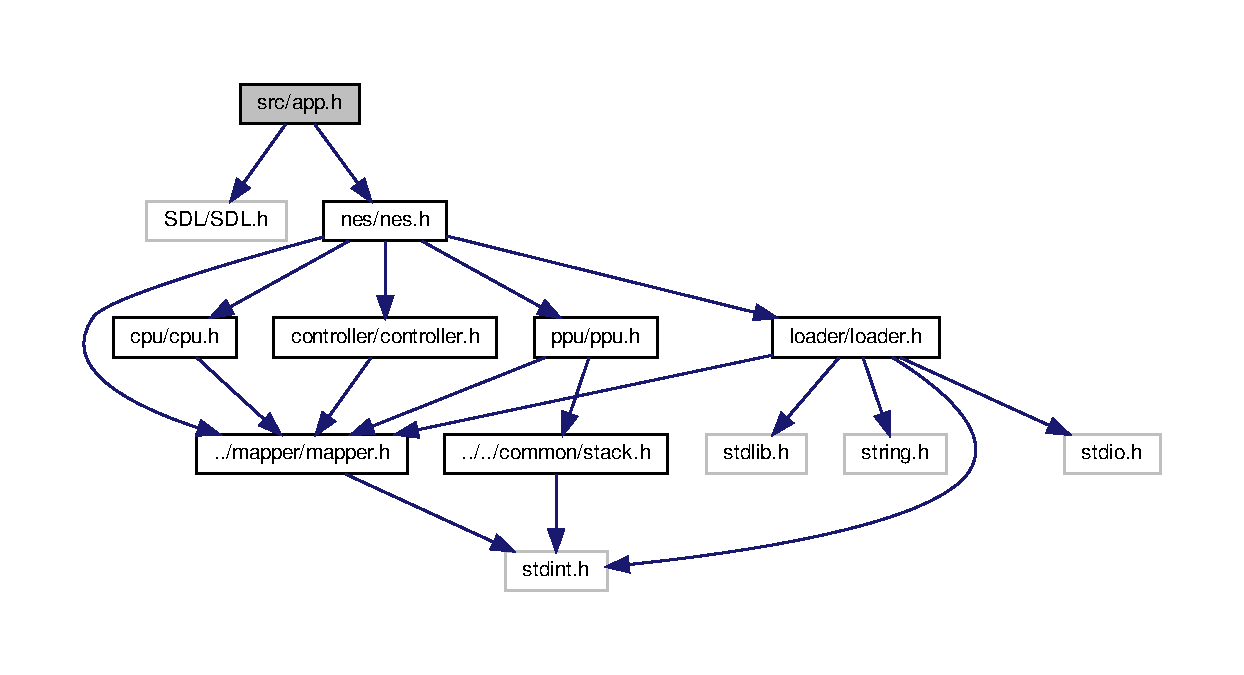
\includegraphics[width=350pt]{app_8h__incl}
\end{center}
\end{figure}
\subsection*{Data Structures}
\begin{DoxyCompactItemize}
\item 
struct \hyperlink{struct_app}{App}
\begin{DoxyCompactList}\small\item\em Hold application data. \end{DoxyCompactList}\end{DoxyCompactItemize}
\subsection*{Macros}
\begin{DoxyCompactItemize}
\item 
\mbox{\Hypertarget{app_8h_a75ffb1897670af90b6941ea94114a3b5}\label{app_8h_a75ffb1897670af90b6941ea94114a3b5}} 
\#define {\bfseries T\+I\+C\+K\+\_\+\+I\+N\+T\+E\+R\+V\+AL}~16
\end{DoxyCompactItemize}
\subsection*{Functions}
\begin{DoxyCompactItemize}
\item 
uint8\+\_\+t \hyperlink{app_8h_ad6a950bf416e156ff9d0fbd3a62a604b}{App\+\_\+\+Init} (\hyperlink{struct_app}{App} $\ast$self, int argc, char $\ast$$\ast$argv)
\begin{DoxyCompactList}\small\item\em Retrieve information from given launch option and init emulator. \end{DoxyCompactList}\item 
uint32\+\_\+t \hyperlink{app_8h_a93325fb7332f0198c36b7679346b31f8}{App\+\_\+\+Time\+Left} (\hyperlink{struct_app}{App} $\ast$self)
\begin{DoxyCompactList}\small\item\em Give time left for delaying screen refresh. \end{DoxyCompactList}\item 
uint8\+\_\+t \hyperlink{app_8h_ae5901525b9cc1482b3cc107290d94ee5}{App\+\_\+\+Execute} (\hyperlink{struct_app}{App} $\ast$self)
\begin{DoxyCompactList}\small\item\em Execute application. \end{DoxyCompactList}\end{DoxyCompactItemize}


\subsection{Detailed Description}
header file of \hyperlink{struct_app}{App} using S\+DL 

\begin{DoxyAuthor}{Author}
Dylan Gageot 
\end{DoxyAuthor}
\begin{DoxyVersion}{Version}
1.\+0 
\end{DoxyVersion}
\begin{DoxyDate}{Date}
2019-\/05-\/05 
\end{DoxyDate}


\subsection{Function Documentation}
\mbox{\Hypertarget{app_8h_ae5901525b9cc1482b3cc107290d94ee5}\label{app_8h_ae5901525b9cc1482b3cc107290d94ee5}} 
\index{app.\+h@{app.\+h}!App\+\_\+\+Execute@{App\+\_\+\+Execute}}
\index{App\+\_\+\+Execute@{App\+\_\+\+Execute}!app.\+h@{app.\+h}}
\subsubsection{\texorpdfstring{App\+\_\+\+Execute()}{App\_Execute()}}
{\footnotesize\ttfamily uint8\+\_\+t App\+\_\+\+Execute (\begin{DoxyParamCaption}\item[{\hyperlink{struct_app}{App} $\ast$}]{self }\end{DoxyParamCaption})}



Execute application. 


\begin{DoxyParams}{Parameters}
{\em self} & instance of \hyperlink{struct_app}{App}\\
\hline
\end{DoxyParams}
\begin{DoxyReturn}{Returns}
E\+X\+I\+T\+\_\+\+S\+U\+C\+C\+E\+SS if succeed, E\+X\+I\+T\+\_\+\+F\+A\+I\+L\+U\+RE otherwise 
\end{DoxyReturn}
\mbox{\Hypertarget{app_8h_ad6a950bf416e156ff9d0fbd3a62a604b}\label{app_8h_ad6a950bf416e156ff9d0fbd3a62a604b}} 
\index{app.\+h@{app.\+h}!App\+\_\+\+Init@{App\+\_\+\+Init}}
\index{App\+\_\+\+Init@{App\+\_\+\+Init}!app.\+h@{app.\+h}}
\subsubsection{\texorpdfstring{App\+\_\+\+Init()}{App\_Init()}}
{\footnotesize\ttfamily uint8\+\_\+t App\+\_\+\+Init (\begin{DoxyParamCaption}\item[{\hyperlink{struct_app}{App} $\ast$}]{self,  }\item[{int}]{argc,  }\item[{char $\ast$$\ast$}]{argv }\end{DoxyParamCaption})}



Retrieve information from given launch option and init emulator. 


\begin{DoxyParams}{Parameters}
{\em self} & instance of \hyperlink{struct_app}{App} \\
\hline
{\em argc} & value of argc \\
\hline
{\em argv} & address of argv\\
\hline
\end{DoxyParams}
\begin{DoxyReturn}{Returns}
E\+X\+I\+T\+\_\+\+S\+U\+C\+C\+E\+SS if succeed, E\+X\+I\+T\+\_\+\+F\+A\+I\+L\+U\+RE otherwise 
\end{DoxyReturn}
\mbox{\Hypertarget{app_8h_a93325fb7332f0198c36b7679346b31f8}\label{app_8h_a93325fb7332f0198c36b7679346b31f8}} 
\index{app.\+h@{app.\+h}!App\+\_\+\+Time\+Left@{App\+\_\+\+Time\+Left}}
\index{App\+\_\+\+Time\+Left@{App\+\_\+\+Time\+Left}!app.\+h@{app.\+h}}
\subsubsection{\texorpdfstring{App\+\_\+\+Time\+Left()}{App\_TimeLeft()}}
{\footnotesize\ttfamily uint32\+\_\+t App\+\_\+\+Time\+Left (\begin{DoxyParamCaption}\item[{\hyperlink{struct_app}{App} $\ast$}]{self }\end{DoxyParamCaption})}



Give time left for delaying screen refresh. 


\begin{DoxyParams}{Parameters}
{\em self} & instance of \hyperlink{struct_app}{App}\\
\hline
\end{DoxyParams}
\begin{DoxyReturn}{Returns}
time left 
\end{DoxyReturn}

\hypertarget{keys_8h}{}\section{src/common/keys.h File Reference}
\label{keys_8h}\index{src/common/keys.\+h@{src/common/keys.\+h}}


header file for \hyperlink{struct_keys}{Keys} module  


\subsection*{Data Structures}
\begin{DoxyCompactItemize}
\item 
struct \hyperlink{struct_keys}{Keys}
\begin{DoxyCompactList}\small\item\em Hold string for key name and corresponding S\+D\+LK constant. \end{DoxyCompactList}\end{DoxyCompactItemize}
\subsection*{Functions}
\begin{DoxyCompactItemize}
\item 
uint16\+\_\+t \hyperlink{keys_8h_a2a0ff58f5d97b2bb4c01118a9d421676}{char\+To\+Sdlk} (char $\ast$key)
\begin{DoxyCompactList}\small\item\em Translate string into S\+D\+LK. \end{DoxyCompactList}\item 
char $\ast$ \hyperlink{keys_8h_a0be2fc82ace3d2c63e1abab305c352df}{Sdlk\+To\+Char} (uint16\+\_\+t sdlk)
\begin{DoxyCompactList}\small\item\em Translate S\+D\+LK into string. \end{DoxyCompactList}\item 
int \hyperlink{keys_8h_a767207e3f13e15df6bced0ce34a905d2}{write\+File\+Keys} (char $\ast$name\+File, uint16\+\_\+t $\ast$keys\+Select)
\begin{DoxyCompactList}\small\item\em Write key configuration to a file. \end{DoxyCompactList}\item 
int \hyperlink{keys_8h_a67cd97211bd245f580b3527b20809638}{read\+File\+Keys} (char $\ast$name\+File, uint16\+\_\+t $\ast$keys\+Select)
\begin{DoxyCompactList}\small\item\em Reade key configuration from a file. \end{DoxyCompactList}\item 
int \hyperlink{keys_8h_adb4899500a4f7e4cad9740c5533ca736}{handle\+Keys} (uint16\+\_\+t $\ast$keys\+Select, uint16\+\_\+t $\ast$keys\+Pressed, S\+D\+L\+\_\+\+Event $\ast$event)
\begin{DoxyCompactList}\small\item\em Handle S\+DL key event. \end{DoxyCompactList}\end{DoxyCompactItemize}


\subsection{Detailed Description}
header file for \hyperlink{struct_keys}{Keys} module 

\begin{DoxyAuthor}{Author}
Nicolas Hily 
\end{DoxyAuthor}
\begin{DoxyVersion}{Version}
1.\+0 
\end{DoxyVersion}
\begin{DoxyDate}{Date}
2019-\/05-\/11 
\end{DoxyDate}


\subsection{Function Documentation}
\mbox{\Hypertarget{keys_8h_a2a0ff58f5d97b2bb4c01118a9d421676}\label{keys_8h_a2a0ff58f5d97b2bb4c01118a9d421676}} 
\index{keys.\+h@{keys.\+h}!char\+To\+Sdlk@{char\+To\+Sdlk}}
\index{char\+To\+Sdlk@{char\+To\+Sdlk}!keys.\+h@{keys.\+h}}
\subsubsection{\texorpdfstring{char\+To\+Sdlk()}{charToSdlk()}}
{\footnotesize\ttfamily uint16\+\_\+t char\+To\+Sdlk (\begin{DoxyParamCaption}\item[{char $\ast$}]{key }\end{DoxyParamCaption})}



Translate string into S\+D\+LK. 


\begin{DoxyParams}{Parameters}
{\em key} & name of the key\\
\hline
\end{DoxyParams}
\begin{DoxyReturn}{Returns}
value of the S\+D\+LK constant 
\end{DoxyReturn}
\mbox{\Hypertarget{keys_8h_adb4899500a4f7e4cad9740c5533ca736}\label{keys_8h_adb4899500a4f7e4cad9740c5533ca736}} 
\index{keys.\+h@{keys.\+h}!handle\+Keys@{handle\+Keys}}
\index{handle\+Keys@{handle\+Keys}!keys.\+h@{keys.\+h}}
\subsubsection{\texorpdfstring{handle\+Keys()}{handleKeys()}}
{\footnotesize\ttfamily int handle\+Keys (\begin{DoxyParamCaption}\item[{uint16\+\_\+t $\ast$}]{keys\+Select,  }\item[{uint16\+\_\+t $\ast$}]{keys\+Pressed,  }\item[{S\+D\+L\+\_\+\+Event $\ast$}]{event }\end{DoxyParamCaption})}



Handle S\+DL key event. 


\begin{DoxyParams}{Parameters}
{\em keys\+Select} & array containg key configuration \\
\hline
{\em keys\+Pressed} & keys pressed \\
\hline
{\em event} & S\+DL event\\
\hline
\end{DoxyParams}
\begin{DoxyReturn}{Returns}
1 if app has not been closed, 0 otherwise 
\end{DoxyReturn}
\mbox{\Hypertarget{keys_8h_a67cd97211bd245f580b3527b20809638}\label{keys_8h_a67cd97211bd245f580b3527b20809638}} 
\index{keys.\+h@{keys.\+h}!read\+File\+Keys@{read\+File\+Keys}}
\index{read\+File\+Keys@{read\+File\+Keys}!keys.\+h@{keys.\+h}}
\subsubsection{\texorpdfstring{read\+File\+Keys()}{readFileKeys()}}
{\footnotesize\ttfamily int read\+File\+Keys (\begin{DoxyParamCaption}\item[{char $\ast$}]{name\+File,  }\item[{uint16\+\_\+t $\ast$}]{keys\+Select }\end{DoxyParamCaption})}



Reade key configuration from a file. 


\begin{DoxyParams}{Parameters}
{\em name\+File} & filename \\
\hline
{\em keys\+Select} & array containing S\+D\+LK keys\\
\hline
\end{DoxyParams}
\begin{DoxyReturn}{Returns}
E\+X\+I\+T\+\_\+\+S\+U\+C\+C\+ES if succeed, E\+X\+I\+T\+\_\+\+F\+A\+I\+L\+U\+RE otherwise 
\end{DoxyReturn}
\mbox{\Hypertarget{keys_8h_a0be2fc82ace3d2c63e1abab305c352df}\label{keys_8h_a0be2fc82ace3d2c63e1abab305c352df}} 
\index{keys.\+h@{keys.\+h}!Sdlk\+To\+Char@{Sdlk\+To\+Char}}
\index{Sdlk\+To\+Char@{Sdlk\+To\+Char}!keys.\+h@{keys.\+h}}
\subsubsection{\texorpdfstring{Sdlk\+To\+Char()}{SdlkToChar()}}
{\footnotesize\ttfamily char$\ast$ Sdlk\+To\+Char (\begin{DoxyParamCaption}\item[{uint16\+\_\+t}]{sdlk }\end{DoxyParamCaption})}



Translate S\+D\+LK into string. 


\begin{DoxyParams}{Parameters}
{\em sdlk} & S\+D\+LK code for a key\\
\hline
\end{DoxyParams}
\begin{DoxyReturn}{Returns}
string pointer 
\end{DoxyReturn}
\mbox{\Hypertarget{keys_8h_a767207e3f13e15df6bced0ce34a905d2}\label{keys_8h_a767207e3f13e15df6bced0ce34a905d2}} 
\index{keys.\+h@{keys.\+h}!write\+File\+Keys@{write\+File\+Keys}}
\index{write\+File\+Keys@{write\+File\+Keys}!keys.\+h@{keys.\+h}}
\subsubsection{\texorpdfstring{write\+File\+Keys()}{writeFileKeys()}}
{\footnotesize\ttfamily int write\+File\+Keys (\begin{DoxyParamCaption}\item[{char $\ast$}]{name\+File,  }\item[{uint16\+\_\+t $\ast$}]{keys\+Select }\end{DoxyParamCaption})}



Write key configuration to a file. 


\begin{DoxyParams}{Parameters}
{\em name\+File} & filename \\
\hline
{\em keys\+Select} & array containing S\+D\+LK keys\\
\hline
\end{DoxyParams}
\begin{DoxyReturn}{Returns}
E\+X\+I\+T\+\_\+\+S\+U\+C\+C\+ES if succeed, E\+X\+I\+T\+\_\+\+F\+A\+I\+L\+U\+RE otherwise 
\end{DoxyReturn}

\hypertarget{macro_8h}{}\section{src/common/macro.h File Reference}
\label{macro_8h}\index{src/common/macro.\+h@{src/common/macro.\+h}}


header file of commonly used macro  


\subsection*{Macros}
\begin{DoxyCompactItemize}
\item 
\#define \hyperlink{macro_8h_ab66bafe0e3773f589f4a239eb3aaecff}{E\+R\+R\+O\+R\+\_\+\+M\+SG}(str)
\begin{DoxyCompactList}\small\item\em Error printed to stderr. \end{DoxyCompactList}\item 
\mbox{\Hypertarget{macro_8h_a8e259b680b0b059eca52866ac23cdda0}\label{macro_8h_a8e259b680b0b059eca52866ac23cdda0}} 
\#define \hyperlink{macro_8h_a8e259b680b0b059eca52866ac23cdda0}{V\+A\+L\+U\+E\+\_\+\+IN}(x,  y,  z)~(((x) $>$= (y)) \&\& ((x) $<$= (z)))
\begin{DoxyCompactList}\small\item\em Test if x is between specified values (y and z) \end{DoxyCompactList}\item 
\mbox{\Hypertarget{macro_8h_ac1d216605cd1e279569a984670c5bdc5}\label{macro_8h_ac1d216605cd1e279569a984670c5bdc5}} 
\#define \hyperlink{macro_8h_ac1d216605cd1e279569a984670c5bdc5}{V\+A\+L\+U\+E\+\_\+\+S\+UP}(x,  y)~(((x) $>$= (y)))
\begin{DoxyCompactList}\small\item\em Test if x is superior to y. \end{DoxyCompactList}\item 
\mbox{\Hypertarget{macro_8h_a852cd83f56e754bd6cd22d24b2c23880}\label{macro_8h_a852cd83f56e754bd6cd22d24b2c23880}} 
\#define \hyperlink{macro_8h_a852cd83f56e754bd6cd22d24b2c23880}{V\+A\+L\+U\+E\+\_\+\+I\+NF}(x,  y)~(((x) $<$= (y)))
\begin{DoxyCompactList}\small\item\em Test if x is inferior to y. \end{DoxyCompactList}\end{DoxyCompactItemize}


\subsection{Detailed Description}
header file of commonly used macro 

\begin{DoxyAuthor}{Author}
Dylan Gageot 
\end{DoxyAuthor}
\begin{DoxyVersion}{Version}
1.\+0 
\end{DoxyVersion}
\begin{DoxyDate}{Date}
2019-\/05-\/11 
\end{DoxyDate}


\subsection{Macro Definition Documentation}
\mbox{\Hypertarget{macro_8h_ab66bafe0e3773f589f4a239eb3aaecff}\label{macro_8h_ab66bafe0e3773f589f4a239eb3aaecff}} 
\index{macro.\+h@{macro.\+h}!E\+R\+R\+O\+R\+\_\+\+M\+SG@{E\+R\+R\+O\+R\+\_\+\+M\+SG}}
\index{E\+R\+R\+O\+R\+\_\+\+M\+SG@{E\+R\+R\+O\+R\+\_\+\+M\+SG}!macro.\+h@{macro.\+h}}
\subsubsection{\texorpdfstring{E\+R\+R\+O\+R\+\_\+\+M\+SG}{ERROR\_MSG}}
{\footnotesize\ttfamily \#define E\+R\+R\+O\+R\+\_\+\+M\+SG(\begin{DoxyParamCaption}\item[{}]{str }\end{DoxyParamCaption})}

{\bfseries Value\+:}
\begin{DoxyCode}
fprintf(stderr, \textcolor{stringliteral}{"Error: %s at %s, line %d.\(\backslash\)n"}, str, \(\backslash\)
                        \_\_FILE\_\_, \_\_LINE\_\_);
\end{DoxyCode}


Error printed to stderr. 


\hypertarget{stack_8h}{}\section{src/common/stack.h File Reference}
\label{stack_8h}\index{src/common/stack.\+h@{src/common/stack.\+h}}


header file of \hyperlink{struct_stack}{Stack} module  


{\ttfamily \#include \char`\"{}stdint.\+h\char`\"{}}\newline
Include dependency graph for stack.\+h\+:\nopagebreak
\begin{figure}[H]
\begin{center}
\leavevmode
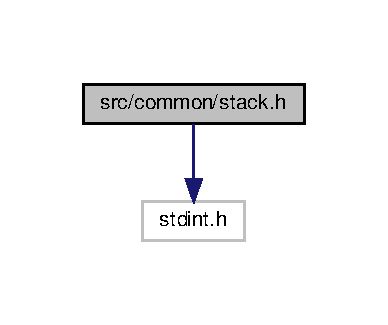
\includegraphics[width=186pt]{stack_8h__incl}
\end{center}
\end{figure}
This graph shows which files directly or indirectly include this file\+:\nopagebreak
\begin{figure}[H]
\begin{center}
\leavevmode
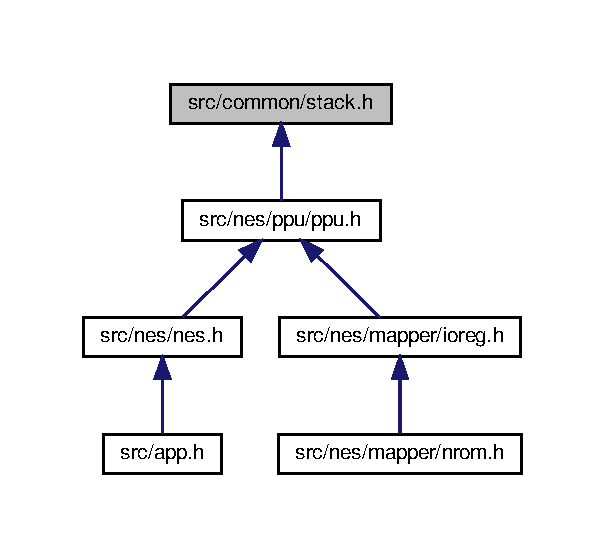
\includegraphics[width=291pt]{stack_8h__dep__incl}
\end{center}
\end{figure}
\subsection*{Data Structures}
\begin{DoxyCompactItemize}
\item 
struct \hyperlink{struct_stack}{Stack}
\begin{DoxyCompactList}\small\item\em Hold stack data and capacity information. \end{DoxyCompactList}\end{DoxyCompactItemize}
\subsection*{Macros}
\begin{DoxyCompactItemize}
\item 
\mbox{\Hypertarget{stack_8h_af24298a5ce56647751e432673282c6e2}\label{stack_8h_af24298a5ce56647751e432673282c6e2}} 
\#define \hyperlink{stack_8h_af24298a5ce56647751e432673282c6e2}{M\+A\+X\+\_\+\+S\+T\+A\+CK}~20
\begin{DoxyCompactList}\small\item\em Max capacity of \hyperlink{struct_stack}{Stack} set to 20. \end{DoxyCompactList}\end{DoxyCompactItemize}
\subsection*{Functions}
\begin{DoxyCompactItemize}
\item 
void \hyperlink{stack_8h_a5607cb7901451341f13970931c6cc880}{Stack\+\_\+\+Init} (\hyperlink{struct_stack}{Stack} $\ast$s)
\begin{DoxyCompactList}\small\item\em Initialize given \hyperlink{struct_stack}{Stack}. \end{DoxyCompactList}\item 
uint8\+\_\+t \hyperlink{stack_8h_af5e65e064f839b2a1836ffb1b1e3b880}{Stack\+\_\+\+Push} (\hyperlink{struct_stack}{Stack} $\ast$s, void $\ast$data)
\begin{DoxyCompactList}\small\item\em Push data to \hyperlink{struct_stack}{Stack}. \end{DoxyCompactList}\item 
void $\ast$ \hyperlink{stack_8h_a20fa129c144b068ab165bd97166842f5}{Stack\+\_\+\+Pop} (\hyperlink{struct_stack}{Stack} $\ast$s)
\begin{DoxyCompactList}\small\item\em Pop data from \hyperlink{struct_stack}{Stack}. \end{DoxyCompactList}\item 
uint8\+\_\+t \hyperlink{stack_8h_aa703f4712602355315d4976a0c8b6a12}{Stack\+\_\+\+Is\+Empty} (\hyperlink{struct_stack}{Stack} $\ast$s)
\begin{DoxyCompactList}\small\item\em Is \hyperlink{struct_stack}{Stack} empty? \end{DoxyCompactList}\end{DoxyCompactItemize}


\subsection{Detailed Description}
header file of \hyperlink{struct_stack}{Stack} module 

\begin{DoxyAuthor}{Author}
Dylan Gageot 
\end{DoxyAuthor}
\begin{DoxyVersion}{Version}

\end{DoxyVersion}
\begin{DoxyDate}{Date}
2019-\/05-\/11
\end{DoxyDate}
Implementation of a F\+I\+LO stack 

\subsection{Function Documentation}
\mbox{\Hypertarget{stack_8h_a5607cb7901451341f13970931c6cc880}\label{stack_8h_a5607cb7901451341f13970931c6cc880}} 
\index{stack.\+h@{stack.\+h}!Stack\+\_\+\+Init@{Stack\+\_\+\+Init}}
\index{Stack\+\_\+\+Init@{Stack\+\_\+\+Init}!stack.\+h@{stack.\+h}}
\subsubsection{\texorpdfstring{Stack\+\_\+\+Init()}{Stack\_Init()}}
{\footnotesize\ttfamily void Stack\+\_\+\+Init (\begin{DoxyParamCaption}\item[{\hyperlink{struct_stack}{Stack} $\ast$}]{s }\end{DoxyParamCaption})}



Initialize given \hyperlink{struct_stack}{Stack}. 


\begin{DoxyParams}{Parameters}
{\em s} & instance of \hyperlink{struct_stack}{Stack} \\
\hline
\end{DoxyParams}
\mbox{\Hypertarget{stack_8h_aa703f4712602355315d4976a0c8b6a12}\label{stack_8h_aa703f4712602355315d4976a0c8b6a12}} 
\index{stack.\+h@{stack.\+h}!Stack\+\_\+\+Is\+Empty@{Stack\+\_\+\+Is\+Empty}}
\index{Stack\+\_\+\+Is\+Empty@{Stack\+\_\+\+Is\+Empty}!stack.\+h@{stack.\+h}}
\subsubsection{\texorpdfstring{Stack\+\_\+\+Is\+Empty()}{Stack\_IsEmpty()}}
{\footnotesize\ttfamily uint8\+\_\+t Stack\+\_\+\+Is\+Empty (\begin{DoxyParamCaption}\item[{\hyperlink{struct_stack}{Stack} $\ast$}]{s }\end{DoxyParamCaption})}



Is \hyperlink{struct_stack}{Stack} empty? 


\begin{DoxyParams}{Parameters}
{\em s} & instance of \hyperlink{struct_stack}{Stack}\\
\hline
\end{DoxyParams}
\begin{DoxyReturn}{Returns}
1 if stack empty, 0 otherwise 
\end{DoxyReturn}
\mbox{\Hypertarget{stack_8h_a20fa129c144b068ab165bd97166842f5}\label{stack_8h_a20fa129c144b068ab165bd97166842f5}} 
\index{stack.\+h@{stack.\+h}!Stack\+\_\+\+Pop@{Stack\+\_\+\+Pop}}
\index{Stack\+\_\+\+Pop@{Stack\+\_\+\+Pop}!stack.\+h@{stack.\+h}}
\subsubsection{\texorpdfstring{Stack\+\_\+\+Pop()}{Stack\_Pop()}}
{\footnotesize\ttfamily void$\ast$ Stack\+\_\+\+Pop (\begin{DoxyParamCaption}\item[{\hyperlink{struct_stack}{Stack} $\ast$}]{s }\end{DoxyParamCaption})}



Pop data from \hyperlink{struct_stack}{Stack}. 


\begin{DoxyParams}{Parameters}
{\em s} & instance of \hyperlink{struct_stack}{Stack}\\
\hline
\end{DoxyParams}
\begin{DoxyReturn}{Returns}
instance of data popped 
\end{DoxyReturn}
\mbox{\Hypertarget{stack_8h_af5e65e064f839b2a1836ffb1b1e3b880}\label{stack_8h_af5e65e064f839b2a1836ffb1b1e3b880}} 
\index{stack.\+h@{stack.\+h}!Stack\+\_\+\+Push@{Stack\+\_\+\+Push}}
\index{Stack\+\_\+\+Push@{Stack\+\_\+\+Push}!stack.\+h@{stack.\+h}}
\subsubsection{\texorpdfstring{Stack\+\_\+\+Push()}{Stack\_Push()}}
{\footnotesize\ttfamily uint8\+\_\+t Stack\+\_\+\+Push (\begin{DoxyParamCaption}\item[{\hyperlink{struct_stack}{Stack} $\ast$}]{s,  }\item[{void $\ast$}]{data }\end{DoxyParamCaption})}



Push data to \hyperlink{struct_stack}{Stack}. 


\begin{DoxyParams}{Parameters}
{\em s} & instance of \hyperlink{struct_stack}{Stack} \\
\hline
{\em data} & instance of data\\
\hline
\end{DoxyParams}
\begin{DoxyReturn}{Returns}
E\+X\+I\+T\+\_\+\+S\+U\+C\+C\+E\+SS if succeed, E\+X\+I\+T\+\_\+\+F\+A\+I\+L\+U\+RE otherwise 
\end{DoxyReturn}

\hypertarget{const_8h}{}\section{src/nes/const.h File Reference}
\label{const_8h}\index{src/nes/const.\+h@{src/nes/const.\+h}}


header file of constants for \hyperlink{struct_n_e_s}{N\+ES} emulation  


\subsection*{Macros}
\begin{DoxyCompactItemize}
\item 
\mbox{\Hypertarget{const_8h_a2b3a08cebe0313da97ccae032dd9d430}\label{const_8h_a2b3a08cebe0313da97ccae032dd9d430}} 
\#define {\bfseries N\+E\+S\+\_\+\+S\+C\+R\+E\+E\+N\+\_\+\+W\+I\+D\+TH}~256
\item 
\mbox{\Hypertarget{const_8h_ab97c175c2977c304ab5e0aee6ea14764}\label{const_8h_ab97c175c2977c304ab5e0aee6ea14764}} 
\#define {\bfseries N\+E\+S\+\_\+\+S\+C\+R\+E\+E\+N\+\_\+\+H\+E\+I\+G\+TH}~240
\item 
\mbox{\Hypertarget{const_8h_a5dd4ef824dac2de1fe0747f9f2917fdd}\label{const_8h_a5dd4ef824dac2de1fe0747f9f2917fdd}} 
\#define {\bfseries A\+D\+D\+R\+\_\+\+P\+P\+U\+C\+T\+RL}~0x2000
\item 
\mbox{\Hypertarget{const_8h_a361a0a196d4185fba104daf400d073f7}\label{const_8h_a361a0a196d4185fba104daf400d073f7}} 
\#define {\bfseries A\+D\+D\+R\+\_\+\+P\+P\+U\+M\+A\+SK}~0x2001
\item 
\mbox{\Hypertarget{const_8h_ae3f8874edd0cc5dc826c9f86d5b45c88}\label{const_8h_ae3f8874edd0cc5dc826c9f86d5b45c88}} 
\#define {\bfseries A\+D\+D\+R\+\_\+\+P\+P\+U\+S\+T\+A\+T\+US}~0x2002
\item 
\mbox{\Hypertarget{const_8h_a6e263054acd55d620958b9e067abfaa4}\label{const_8h_a6e263054acd55d620958b9e067abfaa4}} 
\#define {\bfseries A\+D\+D\+R\+\_\+\+O\+A\+M\+A\+D\+DR}~0x2003
\item 
\mbox{\Hypertarget{const_8h_a5d3670eba4403f70e96f36d550fbbf48}\label{const_8h_a5d3670eba4403f70e96f36d550fbbf48}} 
\#define {\bfseries A\+D\+D\+R\+\_\+\+O\+A\+M\+D\+A\+TA}~0x2004
\item 
\mbox{\Hypertarget{const_8h_a370df7e1312887a0bf954ec7355681e0}\label{const_8h_a370df7e1312887a0bf954ec7355681e0}} 
\#define {\bfseries A\+D\+D\+R\+\_\+\+P\+P\+U\+S\+C\+R\+O\+LL}~0x2005
\item 
\mbox{\Hypertarget{const_8h_a9e269d859ca1437d9528f3d3619f8b93}\label{const_8h_a9e269d859ca1437d9528f3d3619f8b93}} 
\#define {\bfseries A\+D\+D\+R\+\_\+\+P\+P\+U\+A\+D\+DR}~0x2006
\item 
\mbox{\Hypertarget{const_8h_a52da6109c6279f207df36549f959befa}\label{const_8h_a52da6109c6279f207df36549f959befa}} 
\#define {\bfseries A\+D\+D\+R\+\_\+\+P\+P\+U\+D\+A\+TA}~0x2007
\item 
\mbox{\Hypertarget{const_8h_a87d125cc96ace86b09af40fd4a9c9cd6}\label{const_8h_a87d125cc96ace86b09af40fd4a9c9cd6}} 
\#define {\bfseries A\+D\+D\+R\+\_\+\+S\+Q1\+\_\+\+V\+OL}~0x4000
\item 
\mbox{\Hypertarget{const_8h_a6ed1f45ec4edadad6d52135955a6fb11}\label{const_8h_a6ed1f45ec4edadad6d52135955a6fb11}} 
\#define {\bfseries A\+D\+D\+R\+\_\+\+S\+Q1\+\_\+\+S\+W\+E\+EP}~0x4001
\item 
\mbox{\Hypertarget{const_8h_aa63980320b1acb27cd9ce2218601b7b4}\label{const_8h_aa63980320b1acb27cd9ce2218601b7b4}} 
\#define {\bfseries A\+D\+D\+R\+\_\+\+S\+Q1\+\_\+\+LO}~0x4002
\item 
\mbox{\Hypertarget{const_8h_afa3fc5e39142b07a4500c1d583f22673}\label{const_8h_afa3fc5e39142b07a4500c1d583f22673}} 
\#define {\bfseries A\+D\+D\+R\+\_\+\+S\+Q1\+\_\+\+HI}~0x4003
\item 
\mbox{\Hypertarget{const_8h_afc26ea76fb8b5d263ec244b93be42e92}\label{const_8h_afc26ea76fb8b5d263ec244b93be42e92}} 
\#define {\bfseries A\+D\+D\+R\+\_\+\+S\+Q2\+\_\+\+V\+OL}~0x4004
\item 
\mbox{\Hypertarget{const_8h_ad8f3ac97f746eda3930c1e47e06b513c}\label{const_8h_ad8f3ac97f746eda3930c1e47e06b513c}} 
\#define {\bfseries A\+D\+D\+R\+\_\+\+S\+Q2\+\_\+\+S\+W\+E\+EP}~0x4005
\item 
\mbox{\Hypertarget{const_8h_ad03c36270dbe9153196051bc860a2e64}\label{const_8h_ad03c36270dbe9153196051bc860a2e64}} 
\#define {\bfseries A\+D\+D\+R\+\_\+\+S\+Q2\+\_\+\+LO}~0x4006
\item 
\mbox{\Hypertarget{const_8h_a570be3e646bd921662f2d56b44c514f4}\label{const_8h_a570be3e646bd921662f2d56b44c514f4}} 
\#define {\bfseries A\+D\+D\+R\+\_\+\+T\+R\+I\+\_\+\+L\+I\+N\+E\+AR}~0x4008
\item 
\mbox{\Hypertarget{const_8h_ace16cbd1d53d89de52a3a3e4c110e0f0}\label{const_8h_ace16cbd1d53d89de52a3a3e4c110e0f0}} 
\#define {\bfseries A\+D\+D\+R\+\_\+\+T\+R\+I\+\_\+\+LO}~0x400A
\item 
\mbox{\Hypertarget{const_8h_adeb9c4ed78344c0256ebf937bc48d44c}\label{const_8h_adeb9c4ed78344c0256ebf937bc48d44c}} 
\#define {\bfseries A\+D\+D\+R\+\_\+\+T\+R\+I\+\_\+\+HI}~0x400B
\item 
\mbox{\Hypertarget{const_8h_a4f02bb44634003f97bfef48ea2ae6953}\label{const_8h_a4f02bb44634003f97bfef48ea2ae6953}} 
\#define {\bfseries A\+D\+D\+R\+\_\+\+N\+O\+I\+S\+E\+\_\+\+V\+OL}~0x400C
\item 
\mbox{\Hypertarget{const_8h_af74d8d8f513b30af4a911cf4f3cbeef8}\label{const_8h_af74d8d8f513b30af4a911cf4f3cbeef8}} 
\#define {\bfseries A\+D\+D\+R\+\_\+\+N\+O\+I\+S\+E\+\_\+\+LO}~0x400E
\item 
\mbox{\Hypertarget{const_8h_a56f186b964b5171f46fe5ce9931bb302}\label{const_8h_a56f186b964b5171f46fe5ce9931bb302}} 
\#define {\bfseries A\+D\+D\+R\+\_\+\+N\+O\+I\+S\+E\+\_\+\+HI}~0x400F
\item 
\mbox{\Hypertarget{const_8h_a589cda6183b5ef8b1e8389e92cbc7673}\label{const_8h_a589cda6183b5ef8b1e8389e92cbc7673}} 
\#define {\bfseries A\+D\+D\+R\+\_\+\+D\+M\+C\+\_\+\+F\+R\+EQ}~0x4010
\item 
\mbox{\Hypertarget{const_8h_a648f5374458f5090a12500c16b22230e}\label{const_8h_a648f5374458f5090a12500c16b22230e}} 
\#define {\bfseries A\+D\+D\+R\+\_\+\+D\+M\+C\+\_\+\+R\+AW}~0x4011
\item 
\mbox{\Hypertarget{const_8h_a4c7ffcee684aa0eea24b48474a83596a}\label{const_8h_a4c7ffcee684aa0eea24b48474a83596a}} 
\#define {\bfseries A\+D\+D\+R\+\_\+\+D\+M\+C\+\_\+\+S\+T\+A\+RT}~0x4012
\item 
\mbox{\Hypertarget{const_8h_aa15fd9a230e560ed33661b90633cbc47}\label{const_8h_aa15fd9a230e560ed33661b90633cbc47}} 
\#define {\bfseries A\+D\+D\+R\+\_\+\+D\+M\+C\+\_\+\+L\+EN}~0x4013
\item 
\mbox{\Hypertarget{const_8h_a719351bfbded09115dae91e0855fab81}\label{const_8h_a719351bfbded09115dae91e0855fab81}} 
\#define {\bfseries A\+D\+D\+R\+\_\+\+O\+A\+M\+D\+MA}~0x4014
\item 
\mbox{\Hypertarget{const_8h_af7bbdfaf32e30eb03e2f073461a785ff}\label{const_8h_af7bbdfaf32e30eb03e2f073461a785ff}} 
\#define {\bfseries A\+D\+D\+R\+\_\+\+S\+N\+D\+\_\+\+C\+HN}~0x4015
\item 
\mbox{\Hypertarget{const_8h_aed5a6bbc88e54f65446465ef2bb11bd2}\label{const_8h_aed5a6bbc88e54f65446465ef2bb11bd2}} 
\#define {\bfseries A\+D\+D\+R\+\_\+\+J\+O\+Y1}~0x4016
\item 
\mbox{\Hypertarget{const_8h_ae4b93903d5f919fee11b21e8dea6bbbc}\label{const_8h_ae4b93903d5f919fee11b21e8dea6bbbc}} 
\#define {\bfseries A\+D\+D\+R\+\_\+\+J\+O\+Y2}~0x4017
\item 
\mbox{\Hypertarget{const_8h_a27523306a5605ebed1b4b810ee4a89d9}\label{const_8h_a27523306a5605ebed1b4b810ee4a89d9}} 
\#define {\bfseries P\+\_\+\+C\+A\+R\+RY}~0x01
\item 
\mbox{\Hypertarget{const_8h_a86ac1429567770914bfe128c5cb74e41}\label{const_8h_a86ac1429567770914bfe128c5cb74e41}} 
\#define {\bfseries P\+\_\+\+Z\+E\+RO}~0x02
\item 
\mbox{\Hypertarget{const_8h_a7ec2e2e9c5a0cff085a85ae7cd4a5ef0}\label{const_8h_a7ec2e2e9c5a0cff085a85ae7cd4a5ef0}} 
\#define {\bfseries P\+\_\+\+I\+N\+T\+E\+R\+R\+U\+PT}~0x04
\item 
\mbox{\Hypertarget{const_8h_a21da41cb97c450e97b9117d47457bd3d}\label{const_8h_a21da41cb97c450e97b9117d47457bd3d}} 
\#define {\bfseries P\+\_\+\+D\+E\+C\+I\+M\+AL}~0x08
\item 
\mbox{\Hypertarget{const_8h_ab21215fc76a6c7ebe165d3848ad393bd}\label{const_8h_ab21215fc76a6c7ebe165d3848ad393bd}} 
\#define {\bfseries P\+\_\+\+B\+RK}~0x10
\item 
\mbox{\Hypertarget{const_8h_a15141fe5d59efdf035bf8862250c25d7}\label{const_8h_a15141fe5d59efdf035bf8862250c25d7}} 
\#define {\bfseries P\+\_\+\+O\+V\+E\+R\+F\+L\+OW}~0x40
\item 
\mbox{\Hypertarget{const_8h_ad6d97ea38c31d98607fdae94dba5d8be}\label{const_8h_ad6d97ea38c31d98607fdae94dba5d8be}} 
\#define {\bfseries P\+\_\+\+S\+I\+GN}~0x80
\item 
\mbox{\Hypertarget{const_8h_aa587f5047b5d22ef45abc735ae653f93}\label{const_8h_aa587f5047b5d22ef45abc735ae653f93}} 
\#define {\bfseries A\+D\+D\+R\+\_\+\+S\+T\+A\+CK}~0x0100
\item 
\mbox{\Hypertarget{const_8h_a0e52c42e0a4ee950fdfb5e7b8863150a}\label{const_8h_a0e52c42e0a4ee950fdfb5e7b8863150a}} 
\#define {\bfseries S\+I\+Z\+E\+\_\+\+O\+AM}~256
\item 
\mbox{\Hypertarget{const_8h_a34b21d03fb7a353d4ceec451b4830132}\label{const_8h_a34b21d03fb7a353d4ceec451b4830132}} 
\#define {\bfseries S\+I\+Z\+E\+\_\+\+S\+O\+AM}~32
\item 
\mbox{\Hypertarget{const_8h_a98cfe7c8e691ae12842e2c635befb80f}\label{const_8h_a98cfe7c8e691ae12842e2c635befb80f}} 
\#define {\bfseries S\+I\+Z\+E\+\_\+\+C\+O\+L\+O\+R\+\_\+\+P\+A\+L\+E\+T\+TE}~64
\item 
\mbox{\Hypertarget{const_8h_ada199213ce9b7dda2849491c8d857588}\label{const_8h_ada199213ce9b7dda2849491c8d857588}} 
\#define {\bfseries S\+I\+Z\+E\+\_\+\+N\+A\+M\+E\+T\+A\+B\+LE}~0x03\+C0
\item 
\mbox{\Hypertarget{const_8h_aaca38f5c4fdc4be4865e9b8f5cc2a772}\label{const_8h_aaca38f5c4fdc4be4865e9b8f5cc2a772}} 
\#define {\bfseries S\+I\+Z\+E\+\_\+\+A\+T\+T\+R\+I\+B\+U\+TE}~0x0040
\item 
\mbox{\Hypertarget{const_8h_a13272adcc1a4e028d7c0b459256ced40}\label{const_8h_a13272adcc1a4e028d7c0b459256ced40}} 
\#define {\bfseries S\+I\+Z\+E\+\_\+\+P\+A\+T\+T\+E\+RN}~0x1000
\item 
\mbox{\Hypertarget{const_8h_aa78ade133a411afa7a41e6fb0da2f605}\label{const_8h_aa78ade133a411afa7a41e6fb0da2f605}} 
\#define {\bfseries S\+I\+Z\+E\+\_\+\+P\+A\+L\+E\+T\+TE}~0x0010
\item 
\mbox{\Hypertarget{const_8h_af3a85f77922c44bbf8d9cc92c5b1269a}\label{const_8h_af3a85f77922c44bbf8d9cc92c5b1269a}} 
\#define {\bfseries S\+I\+Z\+E\+\_\+\+T\+I\+L\+E\+\_\+\+L\+A\+Y\+ER}~8
\item 
\mbox{\Hypertarget{const_8h_a004a0bd4d35be528654076c4dcdd52d8}\label{const_8h_a004a0bd4d35be528654076c4dcdd52d8}} 
\#define {\bfseries S\+I\+Z\+E\+\_\+\+T\+I\+LE}~16
\item 
\mbox{\Hypertarget{const_8h_a7b8cb2e02ee14f306fc9ed254385a0e0}\label{const_8h_a7b8cb2e02ee14f306fc9ed254385a0e0}} 
\#define {\bfseries P\+R\+E\+R\+E\+N\+D\+E\+R\+\_\+\+S\+C\+A\+N\+L\+I\+NE}~-\/1
\item 
\mbox{\Hypertarget{const_8h_ab9355135d857f0fadc5119e4da3b39b5}\label{const_8h_ab9355135d857f0fadc5119e4da3b39b5}} 
\#define {\bfseries S\+I\+Z\+E\+\_\+\+T\+I\+L\+E\+\_\+\+P\+I\+X\+EL}~8
\item 
\mbox{\Hypertarget{const_8h_ab4a1522687e62b6b4f9b8a4322279b00}\label{const_8h_ab4a1522687e62b6b4f9b8a4322279b00}} 
\#define {\bfseries T\+I\+L\+E\+\_\+\+X\+\_\+\+C\+NT}~(N\+E\+S\+\_\+\+S\+C\+R\+E\+E\+N\+\_\+\+W\+I\+D\+TH/S\+I\+Z\+E\+\_\+\+T\+I\+L\+E\+\_\+\+P\+I\+X\+EL)
\item 
\mbox{\Hypertarget{const_8h_ad469de6fb29f2bc7113afa6ea8f98e22}\label{const_8h_ad469de6fb29f2bc7113afa6ea8f98e22}} 
\#define {\bfseries T\+I\+L\+E\+\_\+\+Y\+\_\+\+C\+NT}~(N\+E\+S\+\_\+\+S\+C\+R\+E\+E\+N\+\_\+\+H\+E\+I\+G\+TH/S\+I\+Z\+E\+\_\+\+T\+I\+L\+E\+\_\+\+P\+I\+X\+EL)
\item 
\mbox{\Hypertarget{const_8h_a4d672dc61e8a4fcb8c52cae6e4950861}\label{const_8h_a4d672dc61e8a4fcb8c52cae6e4950861}} 
\#define {\bfseries S\+P\+R\+\_\+\+S\+O\+A\+M\+\_\+\+C\+NT}~8
\item 
\mbox{\Hypertarget{const_8h_a42b253e72b836e9f6fcfa50b4d42bf20}\label{const_8h_a42b253e72b836e9f6fcfa50b4d42bf20}} 
\#define {\bfseries P\+P\+U\+C\+T\+R\+L\+\_\+\+B\+A\+S\+E\+\_\+\+NT}~0x03
\item 
\mbox{\Hypertarget{const_8h_a4f88c8704e77acc397f2721526ac7bbc}\label{const_8h_a4f88c8704e77acc397f2721526ac7bbc}} 
\#define {\bfseries P\+P\+U\+C\+T\+R\+L\+\_\+\+V\+R\+A\+M\+\_\+\+I\+NC}~0x04
\item 
\mbox{\Hypertarget{const_8h_a8d47a096edeb5f009ea8270405f4dc49}\label{const_8h_a8d47a096edeb5f009ea8270405f4dc49}} 
\#define {\bfseries P\+P\+U\+C\+T\+R\+L\+\_\+\+S\+P\+R\+\_\+\+PT}~0x08
\item 
\mbox{\Hypertarget{const_8h_a926c40fa311702758b14448fe366bdcf}\label{const_8h_a926c40fa311702758b14448fe366bdcf}} 
\#define {\bfseries P\+P\+U\+C\+T\+R\+L\+\_\+\+B\+G\+\_\+\+PT}~0x10
\item 
\mbox{\Hypertarget{const_8h_adc1c18e285a5beb10e8a801d3e0c1c75}\label{const_8h_adc1c18e285a5beb10e8a801d3e0c1c75}} 
\#define {\bfseries P\+P\+U\+C\+T\+R\+L\+\_\+\+S\+P\+R\+\_\+\+S\+I\+ZE}~0x20
\item 
\mbox{\Hypertarget{const_8h_a8e6b6d014b618c014706ea8a4b61d3b3}\label{const_8h_a8e6b6d014b618c014706ea8a4b61d3b3}} 
\#define {\bfseries P\+P\+U\+C\+T\+R\+L\+\_\+\+M\+A\+S\+T\+ER}~0x40
\item 
\mbox{\Hypertarget{const_8h_ad4195c2da9cc37e948b779a3bba574da}\label{const_8h_ad4195c2da9cc37e948b779a3bba574da}} 
\#define {\bfseries P\+P\+U\+C\+T\+R\+L\+\_\+\+N\+MI}~0x80
\item 
\mbox{\Hypertarget{const_8h_af6e68e9f278ff8adb033dd4932d9aeca}\label{const_8h_af6e68e9f278ff8adb033dd4932d9aeca}} 
\#define {\bfseries P\+P\+U\+M\+A\+S\+K\+\_\+\+G\+R\+EY}~0x01
\item 
\mbox{\Hypertarget{const_8h_afdc9908a968e17da267197be3e00ebab}\label{const_8h_afdc9908a968e17da267197be3e00ebab}} 
\#define {\bfseries P\+P\+U\+M\+A\+S\+K\+\_\+\+S\+H\+O\+W\+\_\+\+B\+G\+\_\+8}~0x02
\item 
\mbox{\Hypertarget{const_8h_a9a0999d4a060224c0d8484693ddce5f7}\label{const_8h_a9a0999d4a060224c0d8484693ddce5f7}} 
\#define {\bfseries P\+P\+U\+M\+A\+S\+K\+\_\+\+S\+H\+O\+W\+\_\+\+S\+P\+R\+\_\+8}~0x04
\item 
\mbox{\Hypertarget{const_8h_aaf30bd58f6f863e21f605957d547bdd7}\label{const_8h_aaf30bd58f6f863e21f605957d547bdd7}} 
\#define {\bfseries P\+P\+U\+M\+A\+S\+K\+\_\+\+S\+H\+O\+W\+\_\+\+BG}~0x08
\item 
\mbox{\Hypertarget{const_8h_a73dfa1e321b7b5a3835450c0382f7779}\label{const_8h_a73dfa1e321b7b5a3835450c0382f7779}} 
\#define {\bfseries P\+P\+U\+M\+A\+S\+K\+\_\+\+S\+H\+O\+W\+\_\+\+S\+PR}~0x10
\item 
\mbox{\Hypertarget{const_8h_ab41dcc626b98f557ca739403fc5c3c32}\label{const_8h_ab41dcc626b98f557ca739403fc5c3c32}} 
\#define {\bfseries P\+P\+U\+M\+A\+S\+K\+\_\+\+E\+M\+P\+H\+\_\+\+R\+ED}~0x20
\item 
\mbox{\Hypertarget{const_8h_a023ec617c46740308852ac766bcc74e4}\label{const_8h_a023ec617c46740308852ac766bcc74e4}} 
\#define {\bfseries P\+P\+U\+M\+A\+S\+K\+\_\+\+S\+H\+O\+W\+\_\+\+G\+RN}~0x40
\item 
\mbox{\Hypertarget{const_8h_a31ce9e778699c0ceb8cf6ed3e8143b86}\label{const_8h_a31ce9e778699c0ceb8cf6ed3e8143b86}} 
\#define {\bfseries P\+P\+U\+M\+A\+S\+K\+\_\+\+S\+H\+O\+W\+\_\+\+B\+LU}~0x80
\item 
\mbox{\Hypertarget{const_8h_a673d8c46a6daf0590c9f09f609399393}\label{const_8h_a673d8c46a6daf0590c9f09f609399393}} 
\#define {\bfseries P\+P\+U\+S\+T\+A\+T\+U\+S\+\_\+\+S\+P\+R\+\_\+\+O\+VF}~0x20
\item 
\mbox{\Hypertarget{const_8h_a86ffb1fb6de7a844708c1385c7be7ecf}\label{const_8h_a86ffb1fb6de7a844708c1385c7be7ecf}} 
\#define {\bfseries P\+P\+U\+S\+T\+A\+T\+U\+S\+\_\+\+S\+P\+R\+\_\+\+Z\+E\+RO}~0x40
\item 
\mbox{\Hypertarget{const_8h_a4b59d41c9614ac84f4d721abc6902007}\label{const_8h_a4b59d41c9614ac84f4d721abc6902007}} 
\#define {\bfseries P\+P\+U\+S\+T\+A\+T\+U\+S\+\_\+\+V\+BL}~0x80
\item 
\mbox{\Hypertarget{const_8h_ada74f73ed4bfb02cce788bd47cefcf03}\label{const_8h_ada74f73ed4bfb02cce788bd47cefcf03}} 
\#define {\bfseries I\+N\+D\+E\+X\+\_\+\+O\+A\+M\+\_\+\+Y\+\_\+\+C\+O\+O\+RD}~0
\item 
\mbox{\Hypertarget{const_8h_a1a01c06d0f025237b8c534f78efe8d7a}\label{const_8h_a1a01c06d0f025237b8c534f78efe8d7a}} 
\#define {\bfseries I\+N\+D\+E\+X\+\_\+\+O\+A\+M\+\_\+\+T\+I\+LE}~1
\item 
\mbox{\Hypertarget{const_8h_ab545f90a98ac7e302445bb69a0f91f07}\label{const_8h_ab545f90a98ac7e302445bb69a0f91f07}} 
\#define {\bfseries I\+N\+D\+E\+X\+\_\+\+O\+A\+M\+\_\+\+A\+T\+T\+R\+I\+B\+U\+TE}~2
\item 
\mbox{\Hypertarget{const_8h_ab640e36f34a7953f06a2a2bee4a852d7}\label{const_8h_ab640e36f34a7953f06a2a2bee4a852d7}} 
\#define {\bfseries I\+N\+D\+E\+X\+\_\+\+O\+A\+M\+\_\+\+X\+\_\+\+C\+O\+O\+RD}~3
\item 
\mbox{\Hypertarget{const_8h_abd9748e22eeba7ddcc99e491a95d1402}\label{const_8h_abd9748e22eeba7ddcc99e491a95d1402}} 
\#define {\bfseries O\+A\+M\+\_\+\+A\+T\+T\+R\+I\+B\+U\+T\+E\+\_\+\+P\+A\+L\+E\+T\+TE}~0x03
\item 
\mbox{\Hypertarget{const_8h_aecbcc8ae68a2494832f5e45933cf7805}\label{const_8h_aecbcc8ae68a2494832f5e45933cf7805}} 
\#define {\bfseries O\+A\+M\+\_\+\+A\+T\+T\+R\+I\+B\+U\+T\+E\+\_\+\+P\+R\+I\+O\+T\+IY}~0x20
\item 
\mbox{\Hypertarget{const_8h_a7675078b0940ce759c96ab35ee097106}\label{const_8h_a7675078b0940ce759c96ab35ee097106}} 
\#define {\bfseries O\+A\+M\+\_\+\+A\+T\+T\+R\+I\+B\+U\+T\+E\+\_\+\+F\+L\+I\+P\+\_\+H}~0x40
\item 
\mbox{\Hypertarget{const_8h_a0656d7df880eeb4e6b7739580292935d}\label{const_8h_a0656d7df880eeb4e6b7739580292935d}} 
\#define {\bfseries O\+A\+M\+\_\+\+A\+T\+T\+R\+I\+B\+U\+T\+E\+\_\+\+F\+L\+I\+P\+\_\+V}~0x80
\item 
\mbox{\Hypertarget{const_8h_a0c77f585d93054de46c34fe0c0540f77}\label{const_8h_a0c77f585d93054de46c34fe0c0540f77}} 
\#define {\bfseries O\+A\+M\+\_\+\+A\+T\+T\+R\+I\+B\+U\+T\+E\+\_\+\+F\+L\+IP}~0x\+C0
\item 
\mbox{\Hypertarget{const_8h_aefeb9d8eddb95cad1a7c8bb133ba87c9}\label{const_8h_aefeb9d8eddb95cad1a7c8bb133ba87c9}} 
\#define {\bfseries A\+D\+D\+R\+\_\+\+P\+A\+T\+T\+E\+R\+N\+\_\+1}~0x0000
\item 
\mbox{\Hypertarget{const_8h_a17874c791e2d7b36b9b1ea3dbbb3d4d4}\label{const_8h_a17874c791e2d7b36b9b1ea3dbbb3d4d4}} 
\#define {\bfseries A\+D\+D\+R\+\_\+\+P\+A\+T\+T\+E\+R\+N\+\_\+2}~(A\+D\+D\+R\+\_\+\+P\+A\+T\+T\+E\+R\+N\+\_\+1 + S\+I\+Z\+E\+\_\+\+P\+A\+T\+T\+E\+RN)
\item 
\mbox{\Hypertarget{const_8h_a9ca05fcc478386cb8b4c053d0a104f03}\label{const_8h_a9ca05fcc478386cb8b4c053d0a104f03}} 
\#define {\bfseries A\+D\+D\+R\+\_\+\+N\+A\+M\+E\+T\+A\+B\+L\+E\+\_\+1}~(A\+D\+D\+R\+\_\+\+P\+A\+T\+T\+E\+R\+N\+\_\+2 + S\+I\+Z\+E\+\_\+\+P\+A\+T\+T\+E\+RN)
\item 
\mbox{\Hypertarget{const_8h_a8c4116b6afc2af765599914cdebd63e8}\label{const_8h_a8c4116b6afc2af765599914cdebd63e8}} 
\#define {\bfseries A\+D\+D\+R\+\_\+\+A\+T\+T\+R\+I\+B\+U\+T\+E\+\_\+1}~(A\+D\+D\+R\+\_\+\+N\+A\+M\+E\+T\+A\+B\+L\+E\+\_\+1 + S\+I\+Z\+E\+\_\+\+N\+A\+M\+E\+T\+A\+B\+LE)
\item 
\mbox{\Hypertarget{const_8h_a76a93e8db6b84ff00c2c224b79425a17}\label{const_8h_a76a93e8db6b84ff00c2c224b79425a17}} 
\#define {\bfseries A\+D\+D\+R\+\_\+\+N\+A\+M\+E\+T\+A\+B\+L\+E\+\_\+2}~(A\+D\+D\+R\+\_\+\+A\+T\+T\+R\+I\+B\+U\+T\+E\+\_\+1 + S\+I\+Z\+E\+\_\+\+A\+T\+T\+R\+I\+B\+U\+TE)
\item 
\mbox{\Hypertarget{const_8h_ae3603db167bc1ca561fadb3d2c529efa}\label{const_8h_ae3603db167bc1ca561fadb3d2c529efa}} 
\#define {\bfseries A\+D\+D\+R\+\_\+\+A\+T\+T\+R\+I\+B\+U\+T\+E\+\_\+2}~(A\+D\+D\+R\+\_\+\+N\+A\+M\+E\+T\+A\+B\+L\+E\+\_\+2 + S\+I\+Z\+E\+\_\+\+N\+A\+M\+E\+T\+A\+B\+LE)
\item 
\mbox{\Hypertarget{const_8h_a62d8c43b13360cfa8986bcb0d3b093db}\label{const_8h_a62d8c43b13360cfa8986bcb0d3b093db}} 
\#define {\bfseries A\+D\+D\+R\+\_\+\+N\+A\+M\+E\+T\+A\+B\+L\+E\+\_\+3}~(A\+D\+D\+R\+\_\+\+A\+T\+T\+R\+I\+B\+U\+T\+E\+\_\+2 + S\+I\+Z\+E\+\_\+\+A\+T\+T\+R\+I\+B\+U\+TE)
\item 
\mbox{\Hypertarget{const_8h_aee90faa24bbd9c82495f71aa47220f55}\label{const_8h_aee90faa24bbd9c82495f71aa47220f55}} 
\#define {\bfseries A\+D\+D\+R\+\_\+\+A\+T\+T\+R\+I\+B\+U\+T\+E\+\_\+3}~(A\+D\+D\+R\+\_\+\+N\+A\+M\+E\+T\+A\+B\+L\+E\+\_\+3 + S\+I\+Z\+E\+\_\+\+N\+A\+M\+E\+T\+A\+B\+LE)
\item 
\mbox{\Hypertarget{const_8h_a0cffd1b59589c89ec05494d07c7e4cd0}\label{const_8h_a0cffd1b59589c89ec05494d07c7e4cd0}} 
\#define {\bfseries A\+D\+D\+R\+\_\+\+N\+A\+M\+E\+T\+A\+B\+L\+E\+\_\+4}~(A\+D\+D\+R\+\_\+\+A\+T\+T\+R\+I\+B\+U\+T\+E\+\_\+3 + S\+I\+Z\+E\+\_\+\+A\+T\+T\+R\+I\+B\+U\+TE)
\item 
\mbox{\Hypertarget{const_8h_ad48f12d51f467a8e5c239809bb168e10}\label{const_8h_ad48f12d51f467a8e5c239809bb168e10}} 
\#define {\bfseries A\+D\+D\+R\+\_\+\+A\+T\+T\+R\+I\+B\+U\+T\+E\+\_\+4}~(A\+D\+D\+R\+\_\+\+N\+A\+M\+E\+T\+A\+B\+L\+E\+\_\+4 + S\+I\+Z\+E\+\_\+\+N\+A\+M\+E\+T\+A\+B\+LE)
\item 
\mbox{\Hypertarget{const_8h_a5de822fa541bfdf17fccc590c4acd03c}\label{const_8h_a5de822fa541bfdf17fccc590c4acd03c}} 
\#define {\bfseries A\+D\+D\+R\+\_\+\+P\+A\+L\+E\+T\+T\+E\+\_\+\+BG}~0x3\+F00
\item 
\mbox{\Hypertarget{const_8h_a9b8a65ff58f5bcbf3c7a644aa1301282}\label{const_8h_a9b8a65ff58f5bcbf3c7a644aa1301282}} 
\#define {\bfseries A\+D\+D\+R\+\_\+\+P\+A\+L\+E\+T\+T\+E\+\_\+\+S\+PR}~(A\+D\+D\+R\+\_\+\+P\+A\+L\+E\+T\+T\+E\+\_\+\+BG + S\+I\+Z\+E\+\_\+\+P\+A\+L\+E\+T\+TE)
\end{DoxyCompactItemize}


\subsection{Detailed Description}
header file of constants for \hyperlink{struct_n_e_s}{N\+ES} emulation 

\begin{DoxyAuthor}{Author}
Dylan Gageot 
\end{DoxyAuthor}
\begin{DoxyVersion}{Version}
1.\+0 
\end{DoxyVersion}
\begin{DoxyDate}{Date}
2019-\/05-\/11 
\end{DoxyDate}

\hypertarget{controller_8h}{}\section{src/nes/controller/controller.h File Reference}
\label{controller_8h}\index{src/nes/controller/controller.\+h@{src/nes/controller/controller.\+h}}


header file of \hyperlink{struct_controller}{Controller} module  


{\ttfamily \#include \char`\"{}../mapper/mapper.\+h\char`\"{}}\newline
Include dependency graph for controller.\+h\+:\nopagebreak
\begin{figure}[H]
\begin{center}
\leavevmode
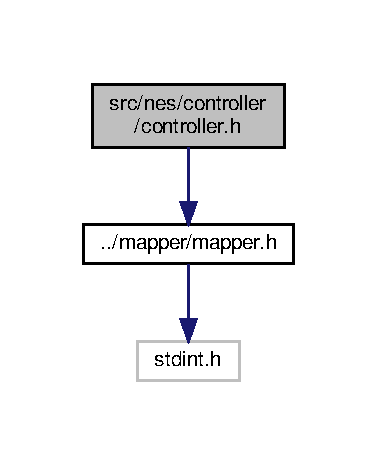
\includegraphics[width=181pt]{controller_8h__incl}
\end{center}
\end{figure}
This graph shows which files directly or indirectly include this file\+:\nopagebreak
\begin{figure}[H]
\begin{center}
\leavevmode
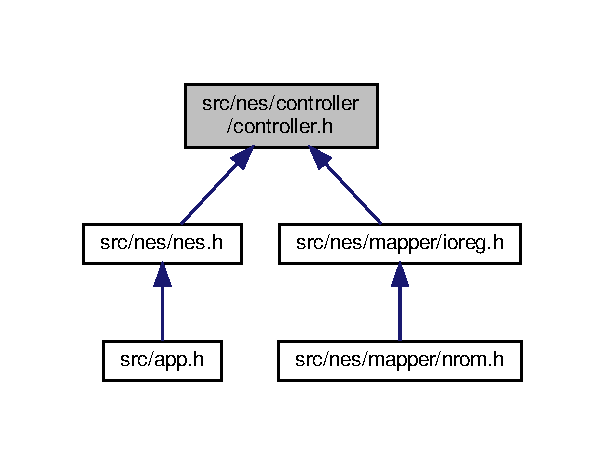
\includegraphics[width=291pt]{controller_8h__dep__incl}
\end{center}
\end{figure}
\subsection*{Data Structures}
\begin{DoxyCompactItemize}
\item 
struct \hyperlink{struct_controller}{Controller}
\begin{DoxyCompactList}\small\item\em Holds necessary variables for the controller emulation to work. Only support the standard joypads. \end{DoxyCompactList}\end{DoxyCompactItemize}
\subsection*{Functions}
\begin{DoxyCompactItemize}
\item 
\hyperlink{struct_controller}{Controller} $\ast$ \hyperlink{controller_8h_af49720e09233955377b151c99a43f64b}{Controller\+\_\+\+Create} (\hyperlink{struct_mapper}{Mapper} $\ast$mapper)
\begin{DoxyCompactList}\small\item\em Allocates memory for controller. \end{DoxyCompactList}\item 
void \hyperlink{controller_8h_a2394059817ac3c97ec0f9560ce16b803}{Controller\+\_\+\+Execute} (\hyperlink{struct_controller}{Controller} $\ast$self, uint16\+\_\+t keys)
\begin{DoxyCompactList}\small\item\em Executes the controller system. \end{DoxyCompactList}\item 
void \hyperlink{controller_8h_a1272b7a3026d1584d085ec1d03e5d2c8}{Controller\+\_\+\+Destroy} (\hyperlink{struct_controller}{Controller} $\ast$self)
\begin{DoxyCompactList}\small\item\em Frees the controller instance\textquotesingle{}s memory. \end{DoxyCompactList}\end{DoxyCompactItemize}


\subsection{Detailed Description}
header file of \hyperlink{struct_controller}{Controller} module 

\begin{DoxyAuthor}{Author}
Nicolas Chabanis 
\end{DoxyAuthor}
\begin{DoxyVersion}{Version}
1.\+0 
\end{DoxyVersion}
\begin{DoxyDate}{Date}
2019-\/05-\/02 
\end{DoxyDate}


\subsection{Function Documentation}
\mbox{\Hypertarget{controller_8h_af49720e09233955377b151c99a43f64b}\label{controller_8h_af49720e09233955377b151c99a43f64b}} 
\index{controller.\+h@{controller.\+h}!Controller\+\_\+\+Create@{Controller\+\_\+\+Create}}
\index{Controller\+\_\+\+Create@{Controller\+\_\+\+Create}!controller.\+h@{controller.\+h}}
\subsubsection{\texorpdfstring{Controller\+\_\+\+Create()}{Controller\_Create()}}
{\footnotesize\ttfamily \hyperlink{struct_controller}{Controller}$\ast$ Controller\+\_\+\+Create (\begin{DoxyParamCaption}\item[{\hyperlink{struct_mapper}{Mapper} $\ast$}]{mapper }\end{DoxyParamCaption})}



Allocates memory for controller. 


\begin{DoxyParams}{Parameters}
{\em pointer} & to the used mapper \\
\hline
\end{DoxyParams}
\begin{DoxyReturn}{Returns}
instance of \hyperlink{struct_controller}{Controller} allocated 
\end{DoxyReturn}
\mbox{\Hypertarget{controller_8h_a1272b7a3026d1584d085ec1d03e5d2c8}\label{controller_8h_a1272b7a3026d1584d085ec1d03e5d2c8}} 
\index{controller.\+h@{controller.\+h}!Controller\+\_\+\+Destroy@{Controller\+\_\+\+Destroy}}
\index{Controller\+\_\+\+Destroy@{Controller\+\_\+\+Destroy}!controller.\+h@{controller.\+h}}
\subsubsection{\texorpdfstring{Controller\+\_\+\+Destroy()}{Controller\_Destroy()}}
{\footnotesize\ttfamily void Controller\+\_\+\+Destroy (\begin{DoxyParamCaption}\item[{\hyperlink{struct_controller}{Controller} $\ast$}]{self }\end{DoxyParamCaption})}



Frees the controller instance\textquotesingle{}s memory. 


\begin{DoxyParams}{Parameters}
{\em self} & instance of the \hyperlink{struct_controller}{Controller} \\
\hline
\end{DoxyParams}
\mbox{\Hypertarget{controller_8h_a2394059817ac3c97ec0f9560ce16b803}\label{controller_8h_a2394059817ac3c97ec0f9560ce16b803}} 
\index{controller.\+h@{controller.\+h}!Controller\+\_\+\+Execute@{Controller\+\_\+\+Execute}}
\index{Controller\+\_\+\+Execute@{Controller\+\_\+\+Execute}!controller.\+h@{controller.\+h}}
\subsubsection{\texorpdfstring{Controller\+\_\+\+Execute()}{Controller\_Execute()}}
{\footnotesize\ttfamily void Controller\+\_\+\+Execute (\begin{DoxyParamCaption}\item[{\hyperlink{struct_controller}{Controller} $\ast$}]{self,  }\item[{uint16\+\_\+t}]{keys }\end{DoxyParamCaption})}



Executes the controller system. 


\begin{DoxyParams}{Parameters}
{\em The} & instance of the controller \\
\hline
{\em The} & state of the current pressed keys (2$\ast$8 keys) \\
\hline
\end{DoxyParams}

\hypertarget{cpu_8h}{}\section{src/nes/cpu/cpu.h File Reference}
\label{cpu_8h}\index{src/nes/cpu/cpu.\+h@{src/nes/cpu/cpu.\+h}}


header file of \hyperlink{struct_c_p_u}{C\+PU} module  


{\ttfamily \#include \char`\"{}../mapper/mapper.\+h\char`\"{}}\newline
Include dependency graph for cpu.\+h\+:\nopagebreak
\begin{figure}[H]
\begin{center}
\leavevmode
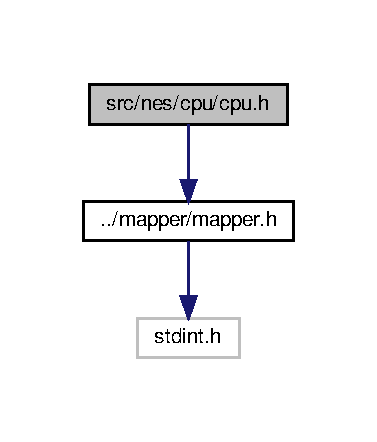
\includegraphics[width=181pt]{cpu_8h__incl}
\end{center}
\end{figure}
This graph shows which files directly or indirectly include this file\+:\nopagebreak
\begin{figure}[H]
\begin{center}
\leavevmode
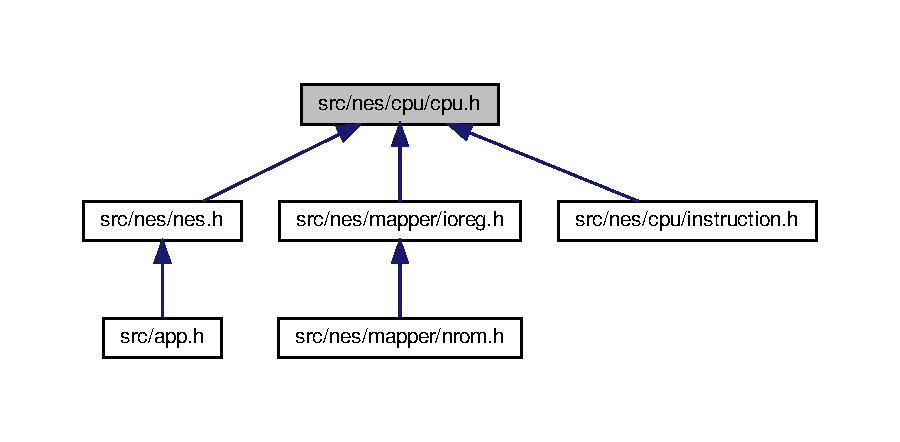
\includegraphics[width=350pt]{cpu_8h__dep__incl}
\end{center}
\end{figure}
\subsection*{Data Structures}
\begin{DoxyCompactItemize}
\item 
struct \hyperlink{struct_c_p_u}{C\+PU}
\begin{DoxyCompactList}\small\item\em Hold \hyperlink{struct_c_p_u}{C\+PU}\textquotesingle{}s register and memory. \end{DoxyCompactList}\end{DoxyCompactItemize}
\subsection*{Macros}
\begin{DoxyCompactItemize}
\item 
\mbox{\Hypertarget{cpu_8h_a5327866481e96fcab2a4c327a9fab75e}\label{cpu_8h_a5327866481e96fcab2a4c327a9fab75e}} 
\#define {\bfseries N\+M\+I\+\_\+\+J\+M\+P\+\_\+\+A\+DD}~0x\+F\+F\+FA
\item 
\mbox{\Hypertarget{cpu_8h_ac7bd2e5bfd09dfc74f62fbecae987f02}\label{cpu_8h_ac7bd2e5bfd09dfc74f62fbecae987f02}} 
\#define {\bfseries R\+E\+S\+\_\+\+J\+M\+P\+\_\+\+A\+DD}~0x\+F\+F\+FC
\item 
\mbox{\Hypertarget{cpu_8h_a523224c2ef57d3e150946f97a17b797a}\label{cpu_8h_a523224c2ef57d3e150946f97a17b797a}} 
\#define {\bfseries I\+R\+Q\+\_\+\+J\+M\+P\+\_\+\+A\+DD}~0x\+F\+F\+FE
\end{DoxyCompactItemize}
\subsection*{Functions}
\begin{DoxyCompactItemize}
\item 
\hyperlink{struct_c_p_u}{C\+PU} $\ast$ \hyperlink{cpu_8h_a0da541cd0a5384beda759a1541959db1}{C\+P\+U\+\_\+\+Create} (\hyperlink{struct_mapper}{Mapper} $\ast$mapper)
\begin{DoxyCompactList}\small\item\em Allocate memory for \hyperlink{struct_c_p_u}{C\+PU} structure. \end{DoxyCompactList}\item 
uint8\+\_\+t \hyperlink{cpu_8h_ae90182d7306c67b8abfb7312ddf62c3b}{C\+P\+U\+\_\+\+Init} (\hyperlink{struct_c_p_u}{C\+PU} $\ast$self)
\begin{DoxyCompactList}\small\item\em Initialize all \hyperlink{struct_c_p_u}{C\+PU} registers (A, X, Y, SP, P and PC) \end{DoxyCompactList}\item 
uint8\+\_\+t \hyperlink{cpu_8h_a9ceedd2706d215552219514eac5dfcae}{C\+P\+U\+\_\+\+Interrupt\+Manager} (\hyperlink{struct_c_p_u}{C\+PU} $\ast$self, uint8\+\_\+t $\ast$context)
\begin{DoxyCompactList}\small\item\em Handle the N\+MI, I\+RQ and B\+RK interrupts. \end{DoxyCompactList}\item 
uint8\+\_\+t \hyperlink{cpu_8h_ab501ecf3e3d7f549067265905fa9556a}{C\+P\+U\+\_\+\+Execute} (\hyperlink{struct_c_p_u}{C\+PU} $\ast$self, uint8\+\_\+t $\ast$context, uint32\+\_\+t $\ast$clock\+Cycle)
\begin{DoxyCompactList}\small\item\em Execute the next instruction. \end{DoxyCompactList}\item 
void \hyperlink{cpu_8h_af1d3bd78687b4d0a1c5fca018287e44c}{C\+P\+U\+\_\+\+Destroy} (\hyperlink{struct_c_p_u}{C\+PU} $\ast$self)
\begin{DoxyCompactList}\small\item\em Free \hyperlink{struct_c_p_u}{C\+PU}\textquotesingle{}s instance. \end{DoxyCompactList}\end{DoxyCompactItemize}


\subsection{Detailed Description}
header file of \hyperlink{struct_c_p_u}{C\+PU} module 

\begin{DoxyAuthor}{Author}
Dylan Gageot 
\end{DoxyAuthor}
\begin{DoxyVersion}{Version}
1.\+0 
\end{DoxyVersion}
\begin{DoxyDate}{Date}
2019-\/02-\/13 
\end{DoxyDate}


\subsection{Function Documentation}
\mbox{\Hypertarget{cpu_8h_a0da541cd0a5384beda759a1541959db1}\label{cpu_8h_a0da541cd0a5384beda759a1541959db1}} 
\index{cpu.\+h@{cpu.\+h}!C\+P\+U\+\_\+\+Create@{C\+P\+U\+\_\+\+Create}}
\index{C\+P\+U\+\_\+\+Create@{C\+P\+U\+\_\+\+Create}!cpu.\+h@{cpu.\+h}}
\subsubsection{\texorpdfstring{C\+P\+U\+\_\+\+Create()}{CPU\_Create()}}
{\footnotesize\ttfamily \hyperlink{struct_c_p_u}{C\+PU}$\ast$ C\+P\+U\+\_\+\+Create (\begin{DoxyParamCaption}\item[{\hyperlink{struct_mapper}{Mapper} $\ast$}]{mapper }\end{DoxyParamCaption})}



Allocate memory for \hyperlink{struct_c_p_u}{C\+PU} structure. 


\begin{DoxyParams}{Parameters}
{\em mapper} & address of \hyperlink{struct_mapper}{Mapper} pointer from \hyperlink{struct_n_e_s}{N\+ES} struct\\
\hline
\end{DoxyParams}
\begin{DoxyReturn}{Returns}
instance of \hyperlink{struct_c_p_u}{C\+PU} allocated 
\end{DoxyReturn}
\mbox{\Hypertarget{cpu_8h_af1d3bd78687b4d0a1c5fca018287e44c}\label{cpu_8h_af1d3bd78687b4d0a1c5fca018287e44c}} 
\index{cpu.\+h@{cpu.\+h}!C\+P\+U\+\_\+\+Destroy@{C\+P\+U\+\_\+\+Destroy}}
\index{C\+P\+U\+\_\+\+Destroy@{C\+P\+U\+\_\+\+Destroy}!cpu.\+h@{cpu.\+h}}
\subsubsection{\texorpdfstring{C\+P\+U\+\_\+\+Destroy()}{CPU\_Destroy()}}
{\footnotesize\ttfamily void C\+P\+U\+\_\+\+Destroy (\begin{DoxyParamCaption}\item[{\hyperlink{struct_c_p_u}{C\+PU} $\ast$}]{self }\end{DoxyParamCaption})}



Free \hyperlink{struct_c_p_u}{C\+PU}\textquotesingle{}s instance. 


\begin{DoxyParams}{Parameters}
{\em self} & \\
\hline
\end{DoxyParams}
\mbox{\Hypertarget{cpu_8h_ab501ecf3e3d7f549067265905fa9556a}\label{cpu_8h_ab501ecf3e3d7f549067265905fa9556a}} 
\index{cpu.\+h@{cpu.\+h}!C\+P\+U\+\_\+\+Execute@{C\+P\+U\+\_\+\+Execute}}
\index{C\+P\+U\+\_\+\+Execute@{C\+P\+U\+\_\+\+Execute}!cpu.\+h@{cpu.\+h}}
\subsubsection{\texorpdfstring{C\+P\+U\+\_\+\+Execute()}{CPU\_Execute()}}
{\footnotesize\ttfamily uint8\+\_\+t C\+P\+U\+\_\+\+Execute (\begin{DoxyParamCaption}\item[{\hyperlink{struct_c_p_u}{C\+PU} $\ast$}]{self,  }\item[{uint8\+\_\+t $\ast$}]{context,  }\item[{uint32\+\_\+t $\ast$}]{clock\+Cycle }\end{DoxyParamCaption})}



Execute the next instruction. 


\begin{DoxyParams}{Parameters}
{\em self} & instance of \hyperlink{struct_c_p_u}{C\+PU} \\
\hline
{\em context} & variable containing interrupt flags \\
\hline
{\em clock\+Cycle} & pointer to clock cycle variable\\
\hline
\end{DoxyParams}
\begin{DoxyReturn}{Returns}
number of clock cycle used to execute the instruction 
\end{DoxyReturn}
\mbox{\Hypertarget{cpu_8h_ae90182d7306c67b8abfb7312ddf62c3b}\label{cpu_8h_ae90182d7306c67b8abfb7312ddf62c3b}} 
\index{cpu.\+h@{cpu.\+h}!C\+P\+U\+\_\+\+Init@{C\+P\+U\+\_\+\+Init}}
\index{C\+P\+U\+\_\+\+Init@{C\+P\+U\+\_\+\+Init}!cpu.\+h@{cpu.\+h}}
\subsubsection{\texorpdfstring{C\+P\+U\+\_\+\+Init()}{CPU\_Init()}}
{\footnotesize\ttfamily uint8\+\_\+t C\+P\+U\+\_\+\+Init (\begin{DoxyParamCaption}\item[{\hyperlink{struct_c_p_u}{C\+PU} $\ast$}]{self }\end{DoxyParamCaption})}



Initialize all \hyperlink{struct_c_p_u}{C\+PU} registers (A, X, Y, SP, P and PC) 


\begin{DoxyParams}{Parameters}
{\em self} & instance of \hyperlink{struct_c_p_u}{C\+PU}\\
\hline
\end{DoxyParams}
\begin{DoxyReturn}{Returns}
E\+X\+I\+T\+\_\+\+S\+U\+C\+C\+E\+SS if succeed, E\+X\+I\+T\+\_\+\+F\+A\+I\+L\+U\+RE otherwise 
\end{DoxyReturn}
\mbox{\Hypertarget{cpu_8h_a9ceedd2706d215552219514eac5dfcae}\label{cpu_8h_a9ceedd2706d215552219514eac5dfcae}} 
\index{cpu.\+h@{cpu.\+h}!C\+P\+U\+\_\+\+Interrupt\+Manager@{C\+P\+U\+\_\+\+Interrupt\+Manager}}
\index{C\+P\+U\+\_\+\+Interrupt\+Manager@{C\+P\+U\+\_\+\+Interrupt\+Manager}!cpu.\+h@{cpu.\+h}}
\subsubsection{\texorpdfstring{C\+P\+U\+\_\+\+Interrupt\+Manager()}{CPU\_InterruptManager()}}
{\footnotesize\ttfamily uint8\+\_\+t C\+P\+U\+\_\+\+Interrupt\+Manager (\begin{DoxyParamCaption}\item[{\hyperlink{struct_c_p_u}{C\+PU} $\ast$}]{self,  }\item[{uint8\+\_\+t $\ast$}]{context }\end{DoxyParamCaption})}



Handle the N\+MI, I\+RQ and B\+RK interrupts. 


\begin{DoxyParams}{Parameters}
{\em self} & instance of \hyperlink{struct_c_p_u}{C\+PU} \\
\hline
{\em context} & variable that contains interrupt flags. xxxx x\+I\+NR \+:
\begin{DoxyItemize}
\item R \+: R\+E\+S\+ET signal detected
\item N \+: N\+MI detected at the end of the previous instruction
\item I \+: I\+RQ detected at the end of the previous instruction
\item x \+: non used bits 
\end{DoxyItemize}\\
\hline
\end{DoxyParams}
\begin{DoxyReturn}{Returns}
number of clock cycle used to execute the instruction 
\end{DoxyReturn}

\hypertarget{instruction_8h}{}\section{src/nes/cpu/instruction.h File Reference}
\label{instruction_8h}\index{src/nes/cpu/instruction.\+h@{src/nes/cpu/instruction.\+h}}


header file of \hyperlink{struct_instruction}{Instruction} module  


{\ttfamily \#include \char`\"{}cpu.\+h\char`\"{}}\newline
Include dependency graph for instruction.\+h\+:\nopagebreak
\begin{figure}[H]
\begin{center}
\leavevmode
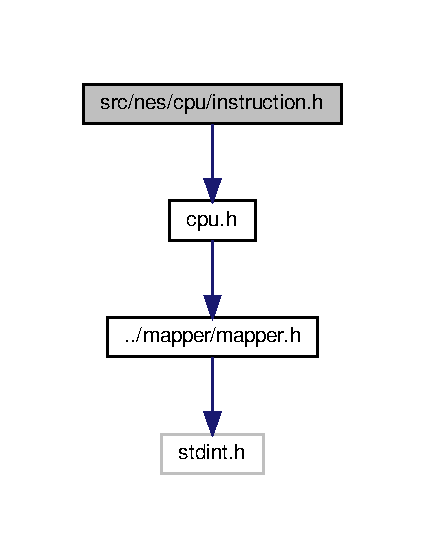
\includegraphics[width=204pt]{instruction_8h__incl}
\end{center}
\end{figure}
\subsection*{Data Structures}
\begin{DoxyCompactItemize}
\item 
struct \hyperlink{struct_opcode}{Opcode}
\begin{DoxyCompactList}\small\item\em Hold instruction function and addressing mode associated. \end{DoxyCompactList}\item 
struct \hyperlink{struct_instruction}{Instruction}
\begin{DoxyCompactList}\small\item\em Hold \hyperlink{struct_opcode}{Opcode} and arguments associated. \end{DoxyCompactList}\end{DoxyCompactItemize}
\subsection*{Macros}
\begin{DoxyCompactItemize}
\item 
\mbox{\Hypertarget{instruction_8h_a39f2333791bc7dbad8245d1abca91507}\label{instruction_8h_a39f2333791bc7dbad8245d1abca91507}} 
\#define {\bfseries D\+M\+A\+\_\+\+O\+FF}~0
\item 
\mbox{\Hypertarget{instruction_8h_afdbde9121c95a15b20c188151164c320}\label{instruction_8h_afdbde9121c95a15b20c188151164c320}} 
\#define {\bfseries D\+M\+A\+\_\+\+ON}~1
\item 
\mbox{\Hypertarget{instruction_8h_a4fdeba015715391e86584e63970bbb62}\label{instruction_8h_a4fdeba015715391e86584e63970bbb62}} 
\#define {\bfseries N\+B\+A\+R\+G\+\_\+\+D\+MA}~0x\+FF
\end{DoxyCompactItemize}
\subsection*{Typedefs}
\begin{DoxyCompactItemize}
\item 
\mbox{\Hypertarget{instruction_8h_a36bbd4522e8a1929f0a16b626c4d9161}\label{instruction_8h_a36bbd4522e8a1929f0a16b626c4d9161}} 
typedef struct \hyperlink{struct_instruction}{Instruction} {\bfseries Instruction}
\end{DoxyCompactItemize}
\subsection*{Enumerations}
\begin{DoxyCompactItemize}
\item 
enum \hyperlink{instruction_8h_aa5cfff0cd9c5ad5ebda7aeecc4a50c2b}{Addressing\+Mode} \{ \newline
\hyperlink{instruction_8h_aa5cfff0cd9c5ad5ebda7aeecc4a50c2ba8054fa474b4ee38123cfeed70397e6f4}{I\+MP} = 0, 
\hyperlink{instruction_8h_aa5cfff0cd9c5ad5ebda7aeecc4a50c2baa6cd1d230aaca43e44f87cd2aab71c83}{A\+CC}, 
\hyperlink{instruction_8h_aa5cfff0cd9c5ad5ebda7aeecc4a50c2bafc8db2219c7a64d05378683b25cf6e82}{Z\+EX}, 
\hyperlink{instruction_8h_aa5cfff0cd9c5ad5ebda7aeecc4a50c2bafedfe8a6fc748d415f1da526b96ec0ea}{Z\+EY}, 
\newline
\hyperlink{instruction_8h_aa5cfff0cd9c5ad5ebda7aeecc4a50c2baded4d1e852e25c6187212be41068b5b0}{I\+NX}, 
\hyperlink{instruction_8h_aa5cfff0cd9c5ad5ebda7aeecc4a50c2bac82a11f742631540ae4e1b48fb405ee6}{I\+NY}, 
\hyperlink{instruction_8h_aa5cfff0cd9c5ad5ebda7aeecc4a50c2baa77e6848bc2c2031677291053c6badaa}{I\+MM}, 
\hyperlink{instruction_8h_aa5cfff0cd9c5ad5ebda7aeecc4a50c2bacb2a8193bc0a747134de34ceb540cdc8}{Z\+ER}, 
\newline
\hyperlink{instruction_8h_aa5cfff0cd9c5ad5ebda7aeecc4a50c2bab2082544bca640e70f0bb74d17a98082}{R\+EL}, 
\hyperlink{instruction_8h_aa5cfff0cd9c5ad5ebda7aeecc4a50c2ba62f7ef0a404defa34640e94940792147}{A\+BS}, 
\hyperlink{instruction_8h_aa5cfff0cd9c5ad5ebda7aeecc4a50c2ba88c7cab15e73ef3fd12422a3c838887a}{A\+BX}, 
\hyperlink{instruction_8h_aa5cfff0cd9c5ad5ebda7aeecc4a50c2bada8a7a910b54a8c3993ff0b659d49b29}{A\+BY}, 
\newline
\hyperlink{instruction_8h_aa5cfff0cd9c5ad5ebda7aeecc4a50c2bae343a5e4c360cbb66537d82b8c7fbd25}{A\+BI}, 
\hyperlink{instruction_8h_aa5cfff0cd9c5ad5ebda7aeecc4a50c2ba4c175fbb65c723226d182dbfd556136a}{N\+UL}
 \}\begin{DoxyCompactList}\small\item\em Mnemonic for every addressing mode. \end{DoxyCompactList}
\end{DoxyCompactItemize}
\subsection*{Functions}
\begin{DoxyCompactItemize}
\item 
uint8\+\_\+t \hyperlink{instruction_8h_aaff869c82a3e5ed485aee64f02521ce9}{Instruction\+\_\+\+D\+MA} (\hyperlink{struct_instruction}{Instruction} $\ast$self, \hyperlink{struct_c_p_u}{C\+PU} $\ast$cpu, uint32\+\_\+t $\ast$clock\+Cycle)
\begin{DoxyCompactList}\small\item\em Manage D\+MA request. \end{DoxyCompactList}\item 
uint8\+\_\+t \hyperlink{instruction_8h_aa86df24b487c14a8d6c7becb117a42b0}{Instruction\+\_\+\+Fetch} (\hyperlink{struct_instruction}{Instruction} $\ast$self, \hyperlink{struct_c_p_u}{C\+PU} $\ast$cpu)
\begin{DoxyCompactList}\small\item\em Fetch and decode instruction from P\+G\+R-\/\+R\+OM. \end{DoxyCompactList}\item 
uint8\+\_\+t \hyperlink{instruction_8h_aecbf0407f0408c73f8d79cf83e9e5059}{Instruction\+\_\+\+Resolve} (\hyperlink{struct_instruction}{Instruction} $\ast$self, \hyperlink{struct_c_p_u}{C\+PU} $\ast$cpu)
\begin{DoxyCompactList}\small\item\em Get the data to execute the instruction. \end{DoxyCompactList}\item 
void \hyperlink{instruction_8h_a328bbc59237bfea408b3384cbf0fb21d}{Instruction\+\_\+\+Print\+Log} (\hyperlink{struct_instruction}{Instruction} $\ast$self, \hyperlink{struct_c_p_u}{C\+PU} $\ast$cpu, uint32\+\_\+t clock\+Cycle)
\begin{DoxyCompactList}\small\item\em Print instruction. \end{DoxyCompactList}\item 
\hyperlink{struct_opcode}{Opcode} \hyperlink{instruction_8h_a4a1ed2a7814e7efe547e78246374fe5e}{Opcode\+\_\+\+Get} (uint8\+\_\+t index)
\begin{DoxyCompactList}\small\item\em Function to use opcode L\+UT in unit-\/test. \end{DoxyCompactList}\item 
\mbox{\Hypertarget{instruction_8h_afef859bd0709445d815175935cb877a5}\label{instruction_8h_afef859bd0709445d815175935cb877a5}} 
void \hyperlink{instruction_8h_afef859bd0709445d815175935cb877a5}{\+\_\+\+S\+E\+T\+\_\+\+S\+I\+GN} (\hyperlink{struct_c_p_u}{C\+PU} $\ast$cpu, uint8\+\_\+t $\ast$src)
\begin{DoxyCompactList}\small\item\em Useful function to ease implementation of the following instructions. \end{DoxyCompactList}\item 
\mbox{\Hypertarget{instruction_8h_add6f26b2a06e638f7e779ed7b60f4096}\label{instruction_8h_add6f26b2a06e638f7e779ed7b60f4096}} 
void {\bfseries \+\_\+\+S\+E\+T\+\_\+\+Z\+E\+RO} (\hyperlink{struct_c_p_u}{C\+PU} $\ast$cpu, uint8\+\_\+t $\ast$src)
\item 
\mbox{\Hypertarget{instruction_8h_ad412dac6bce7a10306dbb79609b5ec86}\label{instruction_8h_ad412dac6bce7a10306dbb79609b5ec86}} 
void {\bfseries \+\_\+\+S\+E\+T\+\_\+\+C\+A\+R\+RY} (\hyperlink{struct_c_p_u}{C\+PU} $\ast$cpu, uint8\+\_\+t cond)
\item 
\mbox{\Hypertarget{instruction_8h_a02c87ffda2dda1534a8f8645e71c4a46}\label{instruction_8h_a02c87ffda2dda1534a8f8645e71c4a46}} 
void {\bfseries \+\_\+\+S\+E\+T\+\_\+\+O\+V\+E\+R\+F\+L\+OW} (\hyperlink{struct_c_p_u}{C\+PU} $\ast$cpu, uint8\+\_\+t cond)
\item 
\mbox{\Hypertarget{instruction_8h_abb885dbe0db2acb5b72389c0c95f18ba}\label{instruction_8h_abb885dbe0db2acb5b72389c0c95f18ba}} 
void {\bfseries \+\_\+\+S\+E\+T\+\_\+\+I\+N\+T\+E\+R\+R\+U\+PT} (\hyperlink{struct_c_p_u}{C\+PU} $\ast$cpu)
\item 
\mbox{\Hypertarget{instruction_8h_ad37ec8142e73844e9d2f9c47ea6bfc51}\label{instruction_8h_ad37ec8142e73844e9d2f9c47ea6bfc51}} 
void {\bfseries \+\_\+\+S\+E\+T\+\_\+\+B\+R\+E\+AK} (\hyperlink{struct_c_p_u}{C\+PU} $\ast$cpu)
\item 
\mbox{\Hypertarget{instruction_8h_aa6f7fb63c2bc60d926b561b5b3ac30df}\label{instruction_8h_aa6f7fb63c2bc60d926b561b5b3ac30df}} 
uint16\+\_\+t {\bfseries \+\_\+\+R\+E\+L\+\_\+\+A\+D\+DR} (\hyperlink{struct_c_p_u}{C\+PU} $\ast$cpu, int8\+\_\+t $\ast$src)
\item 
\mbox{\Hypertarget{instruction_8h_a2183e8da42bd22ac8bc65be84c1f2b4a}\label{instruction_8h_a2183e8da42bd22ac8bc65be84c1f2b4a}} 
void {\bfseries \+\_\+\+S\+E\+T\+\_\+\+SR} (\hyperlink{struct_c_p_u}{C\+PU} $\ast$cpu, uint8\+\_\+t $\ast$src)
\item 
\mbox{\Hypertarget{instruction_8h_a2e0160c9c5b0b9d40b3102cb8b380ea4}\label{instruction_8h_a2e0160c9c5b0b9d40b3102cb8b380ea4}} 
uint8\+\_\+t {\bfseries \+\_\+\+G\+E\+T\+\_\+\+SR} (\hyperlink{struct_c_p_u}{C\+PU} $\ast$cpu)
\item 
\mbox{\Hypertarget{instruction_8h_a94a6c92b20d47c13bfb4386b30e3c860}\label{instruction_8h_a94a6c92b20d47c13bfb4386b30e3c860}} 
uint8\+\_\+t {\bfseries \+\_\+\+P\+U\+LL} (\hyperlink{struct_c_p_u}{C\+PU} $\ast$cpu)
\item 
\mbox{\Hypertarget{instruction_8h_a114a8307734a41cf8f878b0bacd607d5}\label{instruction_8h_a114a8307734a41cf8f878b0bacd607d5}} 
void {\bfseries \+\_\+\+P\+U\+SH} (\hyperlink{struct_c_p_u}{C\+PU} $\ast$cpu, uint8\+\_\+t $\ast$src)
\item 
\mbox{\Hypertarget{instruction_8h_aece1667bdade8b61105fe8fd4004acea}\label{instruction_8h_aece1667bdade8b61105fe8fd4004acea}} 
uint8\+\_\+t $\ast$ {\bfseries \+\_\+\+L\+O\+AD} (\hyperlink{struct_c_p_u}{C\+PU} $\ast$cpu, uint16\+\_\+t address)
\item 
\mbox{\Hypertarget{instruction_8h_aa2256dac0326056d75503aeaa6973abc}\label{instruction_8h_aa2256dac0326056d75503aeaa6973abc}} 
void {\bfseries \+\_\+\+S\+T\+O\+RE} (\hyperlink{struct_c_p_u}{C\+PU} $\ast$cpu, uint16\+\_\+t address, uint8\+\_\+t $\ast$src)
\item 
\mbox{\Hypertarget{instruction_8h_a073151f6cf805edb6ab0aa14ecf70d04}\label{instruction_8h_a073151f6cf805edb6ab0aa14ecf70d04}} 
void {\bfseries \+\_\+\+S\+E\+T\+\_\+\+WR} (\hyperlink{struct_c_p_u}{C\+PU} $\ast$cpu, uint16\+\_\+t address)
\item 
\mbox{\Hypertarget{instruction_8h_a9c0684929b6b7c58fe94680c42db343e}\label{instruction_8h_a9c0684929b6b7c58fe94680c42db343e}} 
uint8\+\_\+t {\bfseries \+\_\+\+I\+F\+\_\+\+C\+A\+R\+RY} (\hyperlink{struct_c_p_u}{C\+PU} $\ast$cpu)
\item 
\mbox{\Hypertarget{instruction_8h_a72af1f61f1bdd97e73e4c45dd5862d53}\label{instruction_8h_a72af1f61f1bdd97e73e4c45dd5862d53}} 
uint8\+\_\+t {\bfseries \+\_\+\+I\+F\+\_\+\+O\+V\+E\+R\+F\+L\+OW} (\hyperlink{struct_c_p_u}{C\+PU} $\ast$cpu)
\item 
\mbox{\Hypertarget{instruction_8h_a56a1693eb76532294b3edc548aa17319}\label{instruction_8h_a56a1693eb76532294b3edc548aa17319}} 
uint8\+\_\+t {\bfseries \+\_\+\+I\+F\+\_\+\+S\+I\+GN} (\hyperlink{struct_c_p_u}{C\+PU} $\ast$cpu)
\item 
\mbox{\Hypertarget{instruction_8h_a48865320ef9b3a1a425ea606234c2e70}\label{instruction_8h_a48865320ef9b3a1a425ea606234c2e70}} 
uint8\+\_\+t {\bfseries \+\_\+\+I\+F\+\_\+\+Z\+E\+RO} (\hyperlink{struct_c_p_u}{C\+PU} $\ast$cpu)
\item 
\mbox{\Hypertarget{instruction_8h_a81e291bfc819808c4adc24aa441d08ae}\label{instruction_8h_a81e291bfc819808c4adc24aa441d08ae}} 
uint8\+\_\+t {\bfseries \+\_\+\+I\+F\+\_\+\+I\+N\+T\+E\+R\+R\+U\+PT} (\hyperlink{struct_c_p_u}{C\+PU} $\ast$cpu)
\item 
\mbox{\Hypertarget{instruction_8h_ad5bfab5e4c2a6d22891ed68ed4bdaf18}\label{instruction_8h_ad5bfab5e4c2a6d22891ed68ed4bdaf18}} 
uint8\+\_\+t {\bfseries \+\_\+\+I\+F\+\_\+\+B\+R\+E\+AK} (\hyperlink{struct_c_p_u}{C\+PU} $\ast$cpu)
\item 
\mbox{\Hypertarget{instruction_8h_a80b3dc6d2e98eafc64f5e52bb7b815b7}\label{instruction_8h_a80b3dc6d2e98eafc64f5e52bb7b815b7}} 
uint8\+\_\+t {\bfseries \+\_\+\+B\+R\+A\+N\+CH} (\hyperlink{struct_c_p_u}{C\+PU} $\ast$cpu, \hyperlink{struct_instruction}{Instruction} $\ast$arg, uint8\+\_\+t cond)
\item 
uint8\+\_\+t \hyperlink{instruction_8h_a03b707d9b2d4827eacc7dc37f9909081}{\+\_\+\+A\+DC} (\hyperlink{struct_c_p_u}{C\+PU} $\ast$cpu, \hyperlink{struct_instruction}{Instruction} $\ast$arg)
\begin{DoxyCompactList}\small\item\em \hyperlink{struct_instruction}{Instruction} set of 6502. \end{DoxyCompactList}\item 
\mbox{\Hypertarget{instruction_8h_aaf700a6a581035f633a19c3955ddb9ca}\label{instruction_8h_aaf700a6a581035f633a19c3955ddb9ca}} 
uint8\+\_\+t {\bfseries \+\_\+\+A\+ND} (\hyperlink{struct_c_p_u}{C\+PU} $\ast$cpu, \hyperlink{struct_instruction}{Instruction} $\ast$arg)
\item 
\mbox{\Hypertarget{instruction_8h_a671344fbb3aabd351376ebf98ba2c1f1}\label{instruction_8h_a671344fbb3aabd351376ebf98ba2c1f1}} 
uint8\+\_\+t {\bfseries \+\_\+\+A\+SL} (\hyperlink{struct_c_p_u}{C\+PU} $\ast$cpu, \hyperlink{struct_instruction}{Instruction} $\ast$arg)
\item 
\mbox{\Hypertarget{instruction_8h_a96ef7e13bd7ea08775c4b8ba623d43e8}\label{instruction_8h_a96ef7e13bd7ea08775c4b8ba623d43e8}} 
uint8\+\_\+t {\bfseries \+\_\+\+B\+CC} (\hyperlink{struct_c_p_u}{C\+PU} $\ast$cpu, \hyperlink{struct_instruction}{Instruction} $\ast$arg)
\item 
\mbox{\Hypertarget{instruction_8h_a25b7c35629206c5f94b7f3474137311a}\label{instruction_8h_a25b7c35629206c5f94b7f3474137311a}} 
uint8\+\_\+t {\bfseries \+\_\+\+B\+CS} (\hyperlink{struct_c_p_u}{C\+PU} $\ast$cpu, \hyperlink{struct_instruction}{Instruction} $\ast$arg)
\item 
\mbox{\Hypertarget{instruction_8h_ac10e90631208d700e082954b2242ade3}\label{instruction_8h_ac10e90631208d700e082954b2242ade3}} 
uint8\+\_\+t {\bfseries \+\_\+\+B\+EQ} (\hyperlink{struct_c_p_u}{C\+PU} $\ast$cpu, \hyperlink{struct_instruction}{Instruction} $\ast$arg)
\item 
\mbox{\Hypertarget{instruction_8h_a48eeb1df625eaa89c9086ccaf6905c3e}\label{instruction_8h_a48eeb1df625eaa89c9086ccaf6905c3e}} 
uint8\+\_\+t {\bfseries \+\_\+\+B\+IT} (\hyperlink{struct_c_p_u}{C\+PU} $\ast$cpu, \hyperlink{struct_instruction}{Instruction} $\ast$arg)
\item 
\mbox{\Hypertarget{instruction_8h_a98fb8654db4b1678a3c1abcf2869baef}\label{instruction_8h_a98fb8654db4b1678a3c1abcf2869baef}} 
uint8\+\_\+t {\bfseries \+\_\+\+B\+MI} (\hyperlink{struct_c_p_u}{C\+PU} $\ast$cpu, \hyperlink{struct_instruction}{Instruction} $\ast$arg)
\item 
\mbox{\Hypertarget{instruction_8h_aeaba7191d44b7878987c8d786d1914eb}\label{instruction_8h_aeaba7191d44b7878987c8d786d1914eb}} 
uint8\+\_\+t {\bfseries \+\_\+\+B\+NE} (\hyperlink{struct_c_p_u}{C\+PU} $\ast$cpu, \hyperlink{struct_instruction}{Instruction} $\ast$arg)
\item 
\mbox{\Hypertarget{instruction_8h_ab335118052c4e5784c463616f7a563a8}\label{instruction_8h_ab335118052c4e5784c463616f7a563a8}} 
uint8\+\_\+t {\bfseries \+\_\+\+B\+PL} (\hyperlink{struct_c_p_u}{C\+PU} $\ast$cpu, \hyperlink{struct_instruction}{Instruction} $\ast$arg)
\item 
\mbox{\Hypertarget{instruction_8h_af4c7e987bdc274b34e94bd9aed774f5f}\label{instruction_8h_af4c7e987bdc274b34e94bd9aed774f5f}} 
uint8\+\_\+t {\bfseries \+\_\+\+B\+RK} (\hyperlink{struct_c_p_u}{C\+PU} $\ast$cpu, \hyperlink{struct_instruction}{Instruction} $\ast$arg)
\item 
\mbox{\Hypertarget{instruction_8h_adf7cfbae9110d7855c6a6adb9dc35765}\label{instruction_8h_adf7cfbae9110d7855c6a6adb9dc35765}} 
uint8\+\_\+t {\bfseries \+\_\+\+B\+VC} (\hyperlink{struct_c_p_u}{C\+PU} $\ast$cpu, \hyperlink{struct_instruction}{Instruction} $\ast$arg)
\item 
\mbox{\Hypertarget{instruction_8h_a00e3c7cca0bb5e5526f62639e2adab29}\label{instruction_8h_a00e3c7cca0bb5e5526f62639e2adab29}} 
uint8\+\_\+t {\bfseries \+\_\+\+B\+VS} (\hyperlink{struct_c_p_u}{C\+PU} $\ast$cpu, \hyperlink{struct_instruction}{Instruction} $\ast$arg)
\item 
\mbox{\Hypertarget{instruction_8h_a7fe07f4bae6e72a6a58f872941161942}\label{instruction_8h_a7fe07f4bae6e72a6a58f872941161942}} 
uint8\+\_\+t {\bfseries \+\_\+\+C\+LC} (\hyperlink{struct_c_p_u}{C\+PU} $\ast$cpu, \hyperlink{struct_instruction}{Instruction} $\ast$arg)
\item 
\mbox{\Hypertarget{instruction_8h_a0054416edcce4a53da39dcfd4a148b7d}\label{instruction_8h_a0054416edcce4a53da39dcfd4a148b7d}} 
uint8\+\_\+t {\bfseries \+\_\+\+C\+LD} (\hyperlink{struct_c_p_u}{C\+PU} $\ast$cpu, \hyperlink{struct_instruction}{Instruction} $\ast$arg)
\item 
\mbox{\Hypertarget{instruction_8h_a00d1bb18b0be19a09c905e51c828fed8}\label{instruction_8h_a00d1bb18b0be19a09c905e51c828fed8}} 
uint8\+\_\+t {\bfseries \+\_\+\+C\+LI} (\hyperlink{struct_c_p_u}{C\+PU} $\ast$cpu, \hyperlink{struct_instruction}{Instruction} $\ast$arg)
\item 
\mbox{\Hypertarget{instruction_8h_aa8d7701a3f6b964aba8b89e78270bcb2}\label{instruction_8h_aa8d7701a3f6b964aba8b89e78270bcb2}} 
uint8\+\_\+t {\bfseries \+\_\+\+C\+LV} (\hyperlink{struct_c_p_u}{C\+PU} $\ast$cpu, \hyperlink{struct_instruction}{Instruction} $\ast$arg)
\item 
\mbox{\Hypertarget{instruction_8h_a4216ae7e1a49c2d293491e469e3d58ae}\label{instruction_8h_a4216ae7e1a49c2d293491e469e3d58ae}} 
uint8\+\_\+t {\bfseries \+\_\+\+C\+MP} (\hyperlink{struct_c_p_u}{C\+PU} $\ast$cpu, \hyperlink{struct_instruction}{Instruction} $\ast$arg)
\item 
\mbox{\Hypertarget{instruction_8h_a8b543b7541c63cdde515457ee50a36c9}\label{instruction_8h_a8b543b7541c63cdde515457ee50a36c9}} 
uint8\+\_\+t {\bfseries \+\_\+\+C\+PX} (\hyperlink{struct_c_p_u}{C\+PU} $\ast$cpu, \hyperlink{struct_instruction}{Instruction} $\ast$arg)
\item 
\mbox{\Hypertarget{instruction_8h_ac3f2daf8cbf328f1e6aa79505908fac4}\label{instruction_8h_ac3f2daf8cbf328f1e6aa79505908fac4}} 
uint8\+\_\+t {\bfseries \+\_\+\+C\+PY} (\hyperlink{struct_c_p_u}{C\+PU} $\ast$cpu, \hyperlink{struct_instruction}{Instruction} $\ast$arg)
\item 
\mbox{\Hypertarget{instruction_8h_a2c32419b8d8db92d7ef139f9462fd330}\label{instruction_8h_a2c32419b8d8db92d7ef139f9462fd330}} 
uint8\+\_\+t {\bfseries \+\_\+\+D\+EC} (\hyperlink{struct_c_p_u}{C\+PU} $\ast$cpu, \hyperlink{struct_instruction}{Instruction} $\ast$arg)
\item 
\mbox{\Hypertarget{instruction_8h_aa5469d57f6b8b5a95d62d3468db08685}\label{instruction_8h_aa5469d57f6b8b5a95d62d3468db08685}} 
uint8\+\_\+t {\bfseries \+\_\+\+D\+EX} (\hyperlink{struct_c_p_u}{C\+PU} $\ast$cpu, \hyperlink{struct_instruction}{Instruction} $\ast$arg)
\item 
\mbox{\Hypertarget{instruction_8h_a86eb2d57bf8dd212053dbb74a5cc422d}\label{instruction_8h_a86eb2d57bf8dd212053dbb74a5cc422d}} 
uint8\+\_\+t {\bfseries \+\_\+\+D\+EY} (\hyperlink{struct_c_p_u}{C\+PU} $\ast$cpu, \hyperlink{struct_instruction}{Instruction} $\ast$arg)
\item 
\mbox{\Hypertarget{instruction_8h_a7bfb11b24c245efbf2236b3b8b252fea}\label{instruction_8h_a7bfb11b24c245efbf2236b3b8b252fea}} 
uint8\+\_\+t {\bfseries \+\_\+\+E\+OR} (\hyperlink{struct_c_p_u}{C\+PU} $\ast$cpu, \hyperlink{struct_instruction}{Instruction} $\ast$arg)
\item 
\mbox{\Hypertarget{instruction_8h_a06be5c2a463e96965d647239742f86d9}\label{instruction_8h_a06be5c2a463e96965d647239742f86d9}} 
uint8\+\_\+t {\bfseries \+\_\+\+I\+NC} (\hyperlink{struct_c_p_u}{C\+PU} $\ast$cpu, \hyperlink{struct_instruction}{Instruction} $\ast$arg)
\item 
\mbox{\Hypertarget{instruction_8h_abec5f4c725985136767ed5c14b23f179}\label{instruction_8h_abec5f4c725985136767ed5c14b23f179}} 
uint8\+\_\+t {\bfseries \+\_\+\+I\+NX} (\hyperlink{struct_c_p_u}{C\+PU} $\ast$cpu, \hyperlink{struct_instruction}{Instruction} $\ast$arg)
\item 
\mbox{\Hypertarget{instruction_8h_a10aabee46553a859b8cc58f618d4b8cc}\label{instruction_8h_a10aabee46553a859b8cc58f618d4b8cc}} 
uint8\+\_\+t {\bfseries \+\_\+\+I\+NY} (\hyperlink{struct_c_p_u}{C\+PU} $\ast$cpu, \hyperlink{struct_instruction}{Instruction} $\ast$arg)
\item 
\mbox{\Hypertarget{instruction_8h_adae60959cbbde07c2be7b7161a4e9c65}\label{instruction_8h_adae60959cbbde07c2be7b7161a4e9c65}} 
uint8\+\_\+t {\bfseries \+\_\+\+J\+MP} (\hyperlink{struct_c_p_u}{C\+PU} $\ast$cpu, \hyperlink{struct_instruction}{Instruction} $\ast$arg)
\item 
\mbox{\Hypertarget{instruction_8h_a852c6087ac318bc38d1af8a632ab7f9d}\label{instruction_8h_a852c6087ac318bc38d1af8a632ab7f9d}} 
uint8\+\_\+t {\bfseries \+\_\+\+J\+SR} (\hyperlink{struct_c_p_u}{C\+PU} $\ast$cpu, \hyperlink{struct_instruction}{Instruction} $\ast$arg)
\item 
\mbox{\Hypertarget{instruction_8h_a49a73c9642d4938852d4bc93c93c3111}\label{instruction_8h_a49a73c9642d4938852d4bc93c93c3111}} 
uint8\+\_\+t {\bfseries \+\_\+\+L\+DA} (\hyperlink{struct_c_p_u}{C\+PU} $\ast$cpu, \hyperlink{struct_instruction}{Instruction} $\ast$arg)
\item 
\mbox{\Hypertarget{instruction_8h_a29591eca6fa2887221563f06f19a6bb5}\label{instruction_8h_a29591eca6fa2887221563f06f19a6bb5}} 
uint8\+\_\+t {\bfseries \+\_\+\+L\+DX} (\hyperlink{struct_c_p_u}{C\+PU} $\ast$cpu, \hyperlink{struct_instruction}{Instruction} $\ast$arg)
\item 
\mbox{\Hypertarget{instruction_8h_a3ebdce21cd6cacacb7a1c94c48488e8f}\label{instruction_8h_a3ebdce21cd6cacacb7a1c94c48488e8f}} 
uint8\+\_\+t {\bfseries \+\_\+\+L\+DY} (\hyperlink{struct_c_p_u}{C\+PU} $\ast$cpu, \hyperlink{struct_instruction}{Instruction} $\ast$arg)
\item 
\mbox{\Hypertarget{instruction_8h_a1644c294d81b170e54ccc13e0f1ad860}\label{instruction_8h_a1644c294d81b170e54ccc13e0f1ad860}} 
uint8\+\_\+t {\bfseries \+\_\+\+L\+SR} (\hyperlink{struct_c_p_u}{C\+PU} $\ast$cpu, \hyperlink{struct_instruction}{Instruction} $\ast$arg)
\item 
\mbox{\Hypertarget{instruction_8h_a90eee5028eda3951c5e0dc5bb50409d1}\label{instruction_8h_a90eee5028eda3951c5e0dc5bb50409d1}} 
uint8\+\_\+t {\bfseries \+\_\+\+N\+OP} (\hyperlink{struct_c_p_u}{C\+PU} $\ast$cpu, \hyperlink{struct_instruction}{Instruction} $\ast$arg)
\item 
\mbox{\Hypertarget{instruction_8h_aec1dc7fa8a127131237f8b74425b34ad}\label{instruction_8h_aec1dc7fa8a127131237f8b74425b34ad}} 
uint8\+\_\+t {\bfseries \+\_\+\+O\+RA} (\hyperlink{struct_c_p_u}{C\+PU} $\ast$cpu, \hyperlink{struct_instruction}{Instruction} $\ast$arg)
\item 
\mbox{\Hypertarget{instruction_8h_a4f0a27884f8f917f40b24d863d2e9bd3}\label{instruction_8h_a4f0a27884f8f917f40b24d863d2e9bd3}} 
uint8\+\_\+t {\bfseries \+\_\+\+P\+HA} (\hyperlink{struct_c_p_u}{C\+PU} $\ast$cpu, \hyperlink{struct_instruction}{Instruction} $\ast$arg)
\item 
\mbox{\Hypertarget{instruction_8h_a21bea7c8f738910b54a1e7538c1df8ed}\label{instruction_8h_a21bea7c8f738910b54a1e7538c1df8ed}} 
uint8\+\_\+t {\bfseries \+\_\+\+P\+HP} (\hyperlink{struct_c_p_u}{C\+PU} $\ast$cpu, \hyperlink{struct_instruction}{Instruction} $\ast$arg)
\item 
\mbox{\Hypertarget{instruction_8h_aad1a5ff191b0c9e20b469e34b0da9eeb}\label{instruction_8h_aad1a5ff191b0c9e20b469e34b0da9eeb}} 
uint8\+\_\+t {\bfseries \+\_\+\+P\+LA} (\hyperlink{struct_c_p_u}{C\+PU} $\ast$cpu, \hyperlink{struct_instruction}{Instruction} $\ast$arg)
\item 
\mbox{\Hypertarget{instruction_8h_a0913efb576f61161c7f4ef49d2bbcdbf}\label{instruction_8h_a0913efb576f61161c7f4ef49d2bbcdbf}} 
uint8\+\_\+t {\bfseries \+\_\+\+P\+LP} (\hyperlink{struct_c_p_u}{C\+PU} $\ast$cpu, \hyperlink{struct_instruction}{Instruction} $\ast$arg)
\item 
\mbox{\Hypertarget{instruction_8h_a414e391e398a44b7ba7bbb51b41b2fd5}\label{instruction_8h_a414e391e398a44b7ba7bbb51b41b2fd5}} 
uint8\+\_\+t {\bfseries \+\_\+\+R\+OL} (\hyperlink{struct_c_p_u}{C\+PU} $\ast$cpu, \hyperlink{struct_instruction}{Instruction} $\ast$arg)
\item 
\mbox{\Hypertarget{instruction_8h_a00d9d91bc3ab592ab82ac17c290572a7}\label{instruction_8h_a00d9d91bc3ab592ab82ac17c290572a7}} 
uint8\+\_\+t {\bfseries \+\_\+\+R\+OR} (\hyperlink{struct_c_p_u}{C\+PU} $\ast$cpu, \hyperlink{struct_instruction}{Instruction} $\ast$arg)
\item 
\mbox{\Hypertarget{instruction_8h_a2e7e0662c5c7e4ece169ce17d97ce944}\label{instruction_8h_a2e7e0662c5c7e4ece169ce17d97ce944}} 
uint8\+\_\+t {\bfseries \+\_\+\+R\+TI} (\hyperlink{struct_c_p_u}{C\+PU} $\ast$cpu, \hyperlink{struct_instruction}{Instruction} $\ast$arg)
\item 
\mbox{\Hypertarget{instruction_8h_afdc1319c0a15060c11de3ea546e76458}\label{instruction_8h_afdc1319c0a15060c11de3ea546e76458}} 
uint8\+\_\+t {\bfseries \+\_\+\+R\+TS} (\hyperlink{struct_c_p_u}{C\+PU} $\ast$cpu, \hyperlink{struct_instruction}{Instruction} $\ast$arg)
\item 
\mbox{\Hypertarget{instruction_8h_aa2cff4ea2221768c5cd1431516ebad8c}\label{instruction_8h_aa2cff4ea2221768c5cd1431516ebad8c}} 
uint8\+\_\+t {\bfseries \+\_\+\+S\+BC} (\hyperlink{struct_c_p_u}{C\+PU} $\ast$cpu, \hyperlink{struct_instruction}{Instruction} $\ast$arg)
\item 
\mbox{\Hypertarget{instruction_8h_a3ae9dbeb7f2acac0d70a635c54695143}\label{instruction_8h_a3ae9dbeb7f2acac0d70a635c54695143}} 
uint8\+\_\+t {\bfseries \+\_\+\+S\+EC} (\hyperlink{struct_c_p_u}{C\+PU} $\ast$cpu, \hyperlink{struct_instruction}{Instruction} $\ast$arg)
\item 
\mbox{\Hypertarget{instruction_8h_a72cf9b2aca3c7063fe19c57b99f6638a}\label{instruction_8h_a72cf9b2aca3c7063fe19c57b99f6638a}} 
uint8\+\_\+t {\bfseries \+\_\+\+S\+ED} (\hyperlink{struct_c_p_u}{C\+PU} $\ast$cpu, \hyperlink{struct_instruction}{Instruction} $\ast$arg)
\item 
\mbox{\Hypertarget{instruction_8h_acba35cef4b26cdb0e9d99d685c87b2fd}\label{instruction_8h_acba35cef4b26cdb0e9d99d685c87b2fd}} 
uint8\+\_\+t {\bfseries \+\_\+\+S\+EI} (\hyperlink{struct_c_p_u}{C\+PU} $\ast$cpu, \hyperlink{struct_instruction}{Instruction} $\ast$arg)
\item 
\mbox{\Hypertarget{instruction_8h_ab4c4fab4074602845976e4095bacbcda}\label{instruction_8h_ab4c4fab4074602845976e4095bacbcda}} 
uint8\+\_\+t {\bfseries \+\_\+\+S\+TA} (\hyperlink{struct_c_p_u}{C\+PU} $\ast$cpu, \hyperlink{struct_instruction}{Instruction} $\ast$arg)
\item 
\mbox{\Hypertarget{instruction_8h_a1479ee5894a39e5b87b09e9d4104e061}\label{instruction_8h_a1479ee5894a39e5b87b09e9d4104e061}} 
uint8\+\_\+t {\bfseries \+\_\+\+S\+TX} (\hyperlink{struct_c_p_u}{C\+PU} $\ast$cpu, \hyperlink{struct_instruction}{Instruction} $\ast$arg)
\item 
\mbox{\Hypertarget{instruction_8h_a404f65149fa054bd08c9f4c9631fc5a7}\label{instruction_8h_a404f65149fa054bd08c9f4c9631fc5a7}} 
uint8\+\_\+t {\bfseries \+\_\+\+S\+TY} (\hyperlink{struct_c_p_u}{C\+PU} $\ast$cpu, \hyperlink{struct_instruction}{Instruction} $\ast$arg)
\item 
\mbox{\Hypertarget{instruction_8h_addb5cba4a6ee241ccbddd8141bf21266}\label{instruction_8h_addb5cba4a6ee241ccbddd8141bf21266}} 
uint8\+\_\+t {\bfseries \+\_\+\+T\+AX} (\hyperlink{struct_c_p_u}{C\+PU} $\ast$cpu, \hyperlink{struct_instruction}{Instruction} $\ast$arg)
\item 
\mbox{\Hypertarget{instruction_8h_adeac6985e3901f30fd58a7620289bd9b}\label{instruction_8h_adeac6985e3901f30fd58a7620289bd9b}} 
uint8\+\_\+t {\bfseries \+\_\+\+T\+AY} (\hyperlink{struct_c_p_u}{C\+PU} $\ast$cpu, \hyperlink{struct_instruction}{Instruction} $\ast$arg)
\item 
\mbox{\Hypertarget{instruction_8h_ae8336cf3caec239a6251a19f30d7c434}\label{instruction_8h_ae8336cf3caec239a6251a19f30d7c434}} 
uint8\+\_\+t {\bfseries \+\_\+\+T\+SX} (\hyperlink{struct_c_p_u}{C\+PU} $\ast$cpu, \hyperlink{struct_instruction}{Instruction} $\ast$arg)
\item 
\mbox{\Hypertarget{instruction_8h_ac6ff3fc8ff1156a41e85f7b272de23d6}\label{instruction_8h_ac6ff3fc8ff1156a41e85f7b272de23d6}} 
uint8\+\_\+t {\bfseries \+\_\+\+T\+XA} (\hyperlink{struct_c_p_u}{C\+PU} $\ast$cpu, \hyperlink{struct_instruction}{Instruction} $\ast$arg)
\item 
\mbox{\Hypertarget{instruction_8h_a5969ffacfa04279ab741eb2262940def}\label{instruction_8h_a5969ffacfa04279ab741eb2262940def}} 
uint8\+\_\+t {\bfseries \+\_\+\+T\+XS} (\hyperlink{struct_c_p_u}{C\+PU} $\ast$cpu, \hyperlink{struct_instruction}{Instruction} $\ast$arg)
\item 
\mbox{\Hypertarget{instruction_8h_af11a7dab63fb1c0fb7fdfeef36fe8bbb}\label{instruction_8h_af11a7dab63fb1c0fb7fdfeef36fe8bbb}} 
uint8\+\_\+t {\bfseries \+\_\+\+T\+YA} (\hyperlink{struct_c_p_u}{C\+PU} $\ast$cpu, \hyperlink{struct_instruction}{Instruction} $\ast$arg)
\end{DoxyCompactItemize}


\subsection{Detailed Description}
header file of \hyperlink{struct_instruction}{Instruction} module 

\begin{DoxyAuthor}{Author}
Dylan Gageot 
\end{DoxyAuthor}
\begin{DoxyVersion}{Version}
1.\+0 
\end{DoxyVersion}
\begin{DoxyDate}{Date}
2019-\/02-\/20 
\end{DoxyDate}


\subsection{Enumeration Type Documentation}
\mbox{\Hypertarget{instruction_8h_aa5cfff0cd9c5ad5ebda7aeecc4a50c2b}\label{instruction_8h_aa5cfff0cd9c5ad5ebda7aeecc4a50c2b}} 
\index{instruction.\+h@{instruction.\+h}!Addressing\+Mode@{Addressing\+Mode}}
\index{Addressing\+Mode@{Addressing\+Mode}!instruction.\+h@{instruction.\+h}}
\subsubsection{\texorpdfstring{Addressing\+Mode}{AddressingMode}}
{\footnotesize\ttfamily enum \hyperlink{instruction_8h_aa5cfff0cd9c5ad5ebda7aeecc4a50c2b}{Addressing\+Mode}}



Mnemonic for every addressing mode. 

\begin{DoxyEnumFields}{Enumerator}
\raisebox{\heightof{T}}[0pt][0pt]{\index{I\+MP@{I\+MP}!instruction.\+h@{instruction.\+h}}\index{instruction.\+h@{instruction.\+h}!I\+MP@{I\+MP}}}\mbox{\Hypertarget{instruction_8h_aa5cfff0cd9c5ad5ebda7aeecc4a50c2ba8054fa474b4ee38123cfeed70397e6f4}\label{instruction_8h_aa5cfff0cd9c5ad5ebda7aeecc4a50c2ba8054fa474b4ee38123cfeed70397e6f4}} 
I\+MP&Implied (0 byte is read in R\+OM) \\
\hline

\raisebox{\heightof{T}}[0pt][0pt]{\index{A\+CC@{A\+CC}!instruction.\+h@{instruction.\+h}}\index{instruction.\+h@{instruction.\+h}!A\+CC@{A\+CC}}}\mbox{\Hypertarget{instruction_8h_aa5cfff0cd9c5ad5ebda7aeecc4a50c2baa6cd1d230aaca43e44f87cd2aab71c83}\label{instruction_8h_aa5cfff0cd9c5ad5ebda7aeecc4a50c2baa6cd1d230aaca43e44f87cd2aab71c83}} 
A\+CC&Accumulator (0 byte is read in R\+OM) \\
\hline

\raisebox{\heightof{T}}[0pt][0pt]{\index{Z\+EX@{Z\+EX}!instruction.\+h@{instruction.\+h}}\index{instruction.\+h@{instruction.\+h}!Z\+EX@{Z\+EX}}}\mbox{\Hypertarget{instruction_8h_aa5cfff0cd9c5ad5ebda7aeecc4a50c2bafc8db2219c7a64d05378683b25cf6e82}\label{instruction_8h_aa5cfff0cd9c5ad5ebda7aeecc4a50c2bafc8db2219c7a64d05378683b25cf6e82}} 
Z\+EX&Zero-\/page Indexed X (1 bytes is read in R\+OM) \\
\hline

\raisebox{\heightof{T}}[0pt][0pt]{\index{Z\+EY@{Z\+EY}!instruction.\+h@{instruction.\+h}}\index{instruction.\+h@{instruction.\+h}!Z\+EY@{Z\+EY}}}\mbox{\Hypertarget{instruction_8h_aa5cfff0cd9c5ad5ebda7aeecc4a50c2bafedfe8a6fc748d415f1da526b96ec0ea}\label{instruction_8h_aa5cfff0cd9c5ad5ebda7aeecc4a50c2bafedfe8a6fc748d415f1da526b96ec0ea}} 
Z\+EY&Zero-\/page Indexed Y (1 bytes is read in R\+OM) \\
\hline

\raisebox{\heightof{T}}[0pt][0pt]{\index{I\+NX@{I\+NX}!instruction.\+h@{instruction.\+h}}\index{instruction.\+h@{instruction.\+h}!I\+NX@{I\+NX}}}\mbox{\Hypertarget{instruction_8h_aa5cfff0cd9c5ad5ebda7aeecc4a50c2baded4d1e852e25c6187212be41068b5b0}\label{instruction_8h_aa5cfff0cd9c5ad5ebda7aeecc4a50c2baded4d1e852e25c6187212be41068b5b0}} 
I\+NX&Pre-\/indexed indirect X (1 bytes is read in R\+OM) \\
\hline

\raisebox{\heightof{T}}[0pt][0pt]{\index{I\+NY@{I\+NY}!instruction.\+h@{instruction.\+h}}\index{instruction.\+h@{instruction.\+h}!I\+NY@{I\+NY}}}\mbox{\Hypertarget{instruction_8h_aa5cfff0cd9c5ad5ebda7aeecc4a50c2bac82a11f742631540ae4e1b48fb405ee6}\label{instruction_8h_aa5cfff0cd9c5ad5ebda7aeecc4a50c2bac82a11f742631540ae4e1b48fb405ee6}} 
I\+NY&Post-\/indexed indirect Y (1 bytes is read in R\+OM) \\
\hline

\raisebox{\heightof{T}}[0pt][0pt]{\index{I\+MM@{I\+MM}!instruction.\+h@{instruction.\+h}}\index{instruction.\+h@{instruction.\+h}!I\+MM@{I\+MM}}}\mbox{\Hypertarget{instruction_8h_aa5cfff0cd9c5ad5ebda7aeecc4a50c2baa77e6848bc2c2031677291053c6badaa}\label{instruction_8h_aa5cfff0cd9c5ad5ebda7aeecc4a50c2baa77e6848bc2c2031677291053c6badaa}} 
I\+MM&Immediate (1 bytes is read in R\+OM) \\
\hline

\raisebox{\heightof{T}}[0pt][0pt]{\index{Z\+ER@{Z\+ER}!instruction.\+h@{instruction.\+h}}\index{instruction.\+h@{instruction.\+h}!Z\+ER@{Z\+ER}}}\mbox{\Hypertarget{instruction_8h_aa5cfff0cd9c5ad5ebda7aeecc4a50c2bacb2a8193bc0a747134de34ceb540cdc8}\label{instruction_8h_aa5cfff0cd9c5ad5ebda7aeecc4a50c2bacb2a8193bc0a747134de34ceb540cdc8}} 
Z\+ER&Zero page (1 bytes is read in R\+OM) \\
\hline

\raisebox{\heightof{T}}[0pt][0pt]{\index{R\+EL@{R\+EL}!instruction.\+h@{instruction.\+h}}\index{instruction.\+h@{instruction.\+h}!R\+EL@{R\+EL}}}\mbox{\Hypertarget{instruction_8h_aa5cfff0cd9c5ad5ebda7aeecc4a50c2bab2082544bca640e70f0bb74d17a98082}\label{instruction_8h_aa5cfff0cd9c5ad5ebda7aeecc4a50c2bab2082544bca640e70f0bb74d17a98082}} 
R\+EL&Relative (1 bytes is read in R\+OM) \\
\hline

\raisebox{\heightof{T}}[0pt][0pt]{\index{A\+BS@{A\+BS}!instruction.\+h@{instruction.\+h}}\index{instruction.\+h@{instruction.\+h}!A\+BS@{A\+BS}}}\mbox{\Hypertarget{instruction_8h_aa5cfff0cd9c5ad5ebda7aeecc4a50c2ba62f7ef0a404defa34640e94940792147}\label{instruction_8h_aa5cfff0cd9c5ad5ebda7aeecc4a50c2ba62f7ef0a404defa34640e94940792147}} 
A\+BS&Absolute (2 bytes is read in R\+OM) \\
\hline

\raisebox{\heightof{T}}[0pt][0pt]{\index{A\+BX@{A\+BX}!instruction.\+h@{instruction.\+h}}\index{instruction.\+h@{instruction.\+h}!A\+BX@{A\+BX}}}\mbox{\Hypertarget{instruction_8h_aa5cfff0cd9c5ad5ebda7aeecc4a50c2ba88c7cab15e73ef3fd12422a3c838887a}\label{instruction_8h_aa5cfff0cd9c5ad5ebda7aeecc4a50c2ba88c7cab15e73ef3fd12422a3c838887a}} 
A\+BX&Indexed X (2 bytes is read in R\+OM) \\
\hline

\raisebox{\heightof{T}}[0pt][0pt]{\index{A\+BY@{A\+BY}!instruction.\+h@{instruction.\+h}}\index{instruction.\+h@{instruction.\+h}!A\+BY@{A\+BY}}}\mbox{\Hypertarget{instruction_8h_aa5cfff0cd9c5ad5ebda7aeecc4a50c2bada8a7a910b54a8c3993ff0b659d49b29}\label{instruction_8h_aa5cfff0cd9c5ad5ebda7aeecc4a50c2bada8a7a910b54a8c3993ff0b659d49b29}} 
A\+BY&Indexed Y (2 bytes is read in R\+OM) \\
\hline

\raisebox{\heightof{T}}[0pt][0pt]{\index{A\+BI@{A\+BI}!instruction.\+h@{instruction.\+h}}\index{instruction.\+h@{instruction.\+h}!A\+BI@{A\+BI}}}\mbox{\Hypertarget{instruction_8h_aa5cfff0cd9c5ad5ebda7aeecc4a50c2bae343a5e4c360cbb66537d82b8c7fbd25}\label{instruction_8h_aa5cfff0cd9c5ad5ebda7aeecc4a50c2bae343a5e4c360cbb66537d82b8c7fbd25}} 
A\+BI&Absolute indirect (2 bytes is read in R\+OM) \\
\hline

\raisebox{\heightof{T}}[0pt][0pt]{\index{N\+UL@{N\+UL}!instruction.\+h@{instruction.\+h}}\index{instruction.\+h@{instruction.\+h}!N\+UL@{N\+UL}}}\mbox{\Hypertarget{instruction_8h_aa5cfff0cd9c5ad5ebda7aeecc4a50c2ba4c175fbb65c723226d182dbfd556136a}\label{instruction_8h_aa5cfff0cd9c5ad5ebda7aeecc4a50c2ba4c175fbb65c723226d182dbfd556136a}} 
N\+UL&Undefined (0 bytes is read in R\+OM) \\
\hline

\end{DoxyEnumFields}


\subsection{Function Documentation}
\mbox{\Hypertarget{instruction_8h_a03b707d9b2d4827eacc7dc37f9909081}\label{instruction_8h_a03b707d9b2d4827eacc7dc37f9909081}} 
\index{instruction.\+h@{instruction.\+h}!\+\_\+\+A\+DC@{\+\_\+\+A\+DC}}
\index{\+\_\+\+A\+DC@{\+\_\+\+A\+DC}!instruction.\+h@{instruction.\+h}}
\subsubsection{\texorpdfstring{\+\_\+\+A\+D\+C()}{\_ADC()}}
{\footnotesize\ttfamily uint8\+\_\+t \+\_\+\+A\+DC (\begin{DoxyParamCaption}\item[{\hyperlink{struct_c_p_u}{C\+PU} $\ast$}]{cpu,  }\item[{\hyperlink{struct_instruction}{Instruction} $\ast$}]{arg }\end{DoxyParamCaption})}



\hyperlink{struct_instruction}{Instruction} set of 6502. 


\begin{DoxyParams}{Parameters}
{\em cpu} & instance of \hyperlink{struct_c_p_u}{C\+PU} \\
\hline
{\em arg} & instance of \hyperlink{struct_instruction}{Instruction}\\
\hline
\end{DoxyParams}
\begin{DoxyReturn}{Returns}
number of \hyperlink{struct_c_p_u}{C\+PU} cycle consumed 
\end{DoxyReturn}
\mbox{\Hypertarget{instruction_8h_aaff869c82a3e5ed485aee64f02521ce9}\label{instruction_8h_aaff869c82a3e5ed485aee64f02521ce9}} 
\index{instruction.\+h@{instruction.\+h}!Instruction\+\_\+\+D\+MA@{Instruction\+\_\+\+D\+MA}}
\index{Instruction\+\_\+\+D\+MA@{Instruction\+\_\+\+D\+MA}!instruction.\+h@{instruction.\+h}}
\subsubsection{\texorpdfstring{Instruction\+\_\+\+D\+M\+A()}{Instruction\_DMA()}}
{\footnotesize\ttfamily uint8\+\_\+t Instruction\+\_\+\+D\+MA (\begin{DoxyParamCaption}\item[{\hyperlink{struct_instruction}{Instruction} $\ast$}]{self,  }\item[{\hyperlink{struct_c_p_u}{C\+PU} $\ast$}]{cpu,  }\item[{uint32\+\_\+t $\ast$}]{clock\+Cycle }\end{DoxyParamCaption})}



Manage D\+MA request. 


\begin{DoxyParams}{Parameters}
{\em self} & instance of \hyperlink{struct_instruction}{Instruction} \\
\hline
{\em cpu} & instance of \hyperlink{struct_c_p_u}{C\+PU}\\
\hline
\end{DoxyParams}
\begin{DoxyReturn}{Returns}
E\+X\+I\+T\+\_\+\+S\+U\+C\+C\+E\+SS if succeed, E\+X\+I\+T\+\_\+\+F\+A\+I\+L\+U\+RE otherwise 
\end{DoxyReturn}
\mbox{\Hypertarget{instruction_8h_aa86df24b487c14a8d6c7becb117a42b0}\label{instruction_8h_aa86df24b487c14a8d6c7becb117a42b0}} 
\index{instruction.\+h@{instruction.\+h}!Instruction\+\_\+\+Fetch@{Instruction\+\_\+\+Fetch}}
\index{Instruction\+\_\+\+Fetch@{Instruction\+\_\+\+Fetch}!instruction.\+h@{instruction.\+h}}
\subsubsection{\texorpdfstring{Instruction\+\_\+\+Fetch()}{Instruction\_Fetch()}}
{\footnotesize\ttfamily uint8\+\_\+t Instruction\+\_\+\+Fetch (\begin{DoxyParamCaption}\item[{\hyperlink{struct_instruction}{Instruction} $\ast$}]{self,  }\item[{\hyperlink{struct_c_p_u}{C\+PU} $\ast$}]{cpu }\end{DoxyParamCaption})}



Fetch and decode instruction from P\+G\+R-\/\+R\+OM. 


\begin{DoxyParams}{Parameters}
{\em self} & instance of \hyperlink{struct_instruction}{Instruction} \\
\hline
{\em cpu} & instance of \hyperlink{struct_c_p_u}{C\+PU}\\
\hline
\end{DoxyParams}
\begin{DoxyReturn}{Returns}
E\+X\+I\+T\+\_\+\+S\+U\+C\+C\+E\+SS if succeed, E\+X\+I\+T\+\_\+\+F\+A\+I\+L\+U\+RE otherwise 
\end{DoxyReturn}
\mbox{\Hypertarget{instruction_8h_a328bbc59237bfea408b3384cbf0fb21d}\label{instruction_8h_a328bbc59237bfea408b3384cbf0fb21d}} 
\index{instruction.\+h@{instruction.\+h}!Instruction\+\_\+\+Print\+Log@{Instruction\+\_\+\+Print\+Log}}
\index{Instruction\+\_\+\+Print\+Log@{Instruction\+\_\+\+Print\+Log}!instruction.\+h@{instruction.\+h}}
\subsubsection{\texorpdfstring{Instruction\+\_\+\+Print\+Log()}{Instruction\_PrintLog()}}
{\footnotesize\ttfamily void Instruction\+\_\+\+Print\+Log (\begin{DoxyParamCaption}\item[{\hyperlink{struct_instruction}{Instruction} $\ast$}]{self,  }\item[{\hyperlink{struct_c_p_u}{C\+PU} $\ast$}]{cpu,  }\item[{uint32\+\_\+t}]{clock\+Cycle }\end{DoxyParamCaption})}



Print instruction. 


\begin{DoxyParams}{Parameters}
{\em self} & instance of \hyperlink{struct_c_p_u}{C\+PU} \\
\hline
{\em inst} & instance of \hyperlink{struct_instruction}{Instruction} \\
\hline
{\em clock\+Cycle} & number of clock cycle needed \\
\hline
\end{DoxyParams}
\mbox{\Hypertarget{instruction_8h_aecbf0407f0408c73f8d79cf83e9e5059}\label{instruction_8h_aecbf0407f0408c73f8d79cf83e9e5059}} 
\index{instruction.\+h@{instruction.\+h}!Instruction\+\_\+\+Resolve@{Instruction\+\_\+\+Resolve}}
\index{Instruction\+\_\+\+Resolve@{Instruction\+\_\+\+Resolve}!instruction.\+h@{instruction.\+h}}
\subsubsection{\texorpdfstring{Instruction\+\_\+\+Resolve()}{Instruction\_Resolve()}}
{\footnotesize\ttfamily uint8\+\_\+t Instruction\+\_\+\+Resolve (\begin{DoxyParamCaption}\item[{\hyperlink{struct_instruction}{Instruction} $\ast$}]{self,  }\item[{\hyperlink{struct_c_p_u}{C\+PU} $\ast$}]{cpu }\end{DoxyParamCaption})}



Get the data to execute the instruction. 


\begin{DoxyParams}{Parameters}
{\em self} & instance of \hyperlink{struct_instruction}{Instruction} \\
\hline
{\em cpu} & instance of \hyperlink{struct_c_p_u}{C\+PU}\\
\hline
\end{DoxyParams}
\begin{DoxyReturn}{Returns}
E\+X\+I\+T\+\_\+\+S\+U\+C\+C\+E\+SS if succeed, E\+X\+I\+T\+\_\+\+F\+A\+I\+L\+U\+RE otherwise 
\end{DoxyReturn}
\mbox{\Hypertarget{instruction_8h_a4a1ed2a7814e7efe547e78246374fe5e}\label{instruction_8h_a4a1ed2a7814e7efe547e78246374fe5e}} 
\index{instruction.\+h@{instruction.\+h}!Opcode\+\_\+\+Get@{Opcode\+\_\+\+Get}}
\index{Opcode\+\_\+\+Get@{Opcode\+\_\+\+Get}!instruction.\+h@{instruction.\+h}}
\subsubsection{\texorpdfstring{Opcode\+\_\+\+Get()}{Opcode\_Get()}}
{\footnotesize\ttfamily \hyperlink{struct_opcode}{Opcode} Opcode\+\_\+\+Get (\begin{DoxyParamCaption}\item[{uint8\+\_\+t}]{index }\end{DoxyParamCaption})}



Function to use opcode L\+UT in unit-\/test. 


\begin{DoxyParams}{Parameters}
{\em index} & index to search from\\
\hline
\end{DoxyParams}
\begin{DoxyReturn}{Returns}
\hyperlink{struct_opcode}{Opcode} struct 
\end{DoxyReturn}

\hypertarget{loader_8h}{}\section{src/nes/loader/loader.h File Reference}
\label{loader_8h}\index{src/nes/loader/loader.\+h@{src/nes/loader/loader.\+h}}


header file of R\+OM loader  


{\ttfamily \#include $<$stdio.\+h$>$}\newline
{\ttfamily \#include $<$stdlib.\+h$>$}\newline
{\ttfamily \#include $<$stdint.\+h$>$}\newline
{\ttfamily \#include $<$string.\+h$>$}\newline
{\ttfamily \#include \char`\"{}../mapper/mapper.\+h\char`\"{}}\newline
Include dependency graph for loader.\+h\+:\nopagebreak
\begin{figure}[H]
\begin{center}
\leavevmode
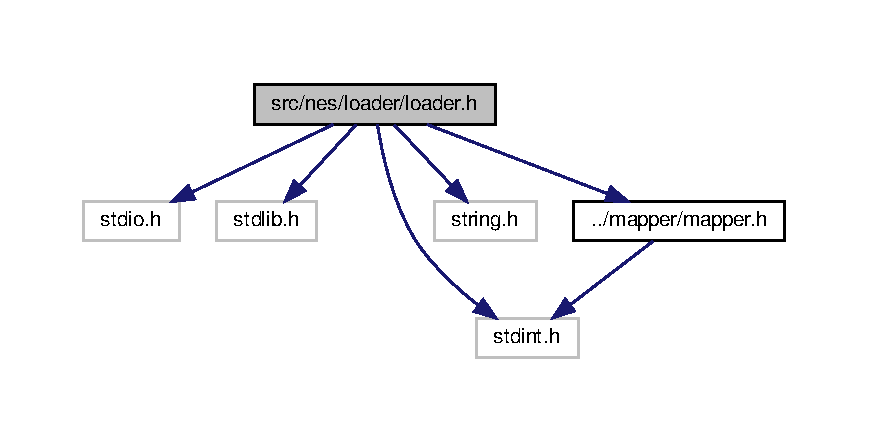
\includegraphics[width=350pt]{loader_8h__incl}
\end{center}
\end{figure}
This graph shows which files directly or indirectly include this file\+:\nopagebreak
\begin{figure}[H]
\begin{center}
\leavevmode
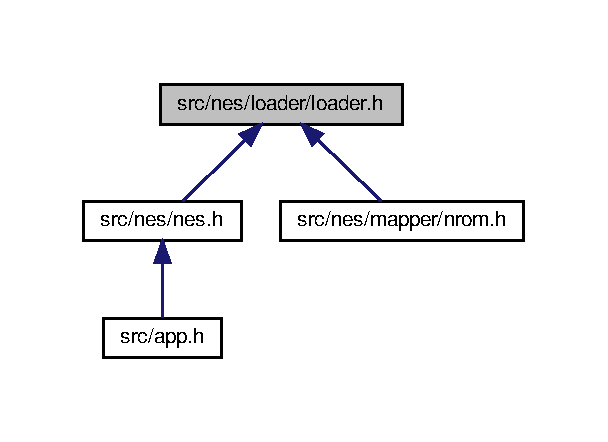
\includegraphics[width=292pt]{loader_8h__dep__incl}
\end{center}
\end{figure}
\subsection*{Data Structures}
\begin{DoxyCompactItemize}
\item 
struct \hyperlink{struct_header}{Header}
\begin{DoxyCompactList}\small\item\em \hyperlink{struct_header}{Header} of a .nes file, modified for programming purposes. \end{DoxyCompactList}\end{DoxyCompactItemize}
\subsection*{Macros}
\begin{DoxyCompactItemize}
\item 
\mbox{\Hypertarget{loader_8h_a73984f580ef5cbdbc1d0b35d7e00ea69}\label{loader_8h_a73984f580ef5cbdbc1d0b35d7e00ea69}} 
\#define \hyperlink{loader_8h_a73984f580ef5cbdbc1d0b35d7e00ea69}{M\+A\+P\+P\+E\+R\+\_\+\+T\+O\+T\+AL}~26
\begin{DoxyCompactList}\small\item\em Number of mapper. \end{DoxyCompactList}\end{DoxyCompactItemize}
\subsection*{Functions}
\begin{DoxyCompactItemize}
\item 
void \hyperlink{loader_8h_a09f39eacdf4f00f25dc30c8f94e3834e}{fill\+Header} (\hyperlink{struct_header}{Header} $\ast$header, uint8\+\_\+t $\ast$h)
\begin{DoxyCompactList}\small\item\em Fills the header with its attributes. \end{DoxyCompactList}\item 
\hyperlink{struct_mapper}{Mapper} $\ast$ \hyperlink{loader_8h_ac30622c837cd4528cc01201cd2268153}{load\+R\+OM} (char $\ast$filename)
\begin{DoxyCompactList}\small\item\em Load R\+OM into \hyperlink{struct_mapper}{Mapper} structure. \end{DoxyCompactList}\end{DoxyCompactItemize}


\subsection{Detailed Description}
header file of R\+OM loader 

\begin{DoxyAuthor}{Author}
Nicolas Chabanis 
\end{DoxyAuthor}
\begin{DoxyVersion}{Version}
1.\+0 
\end{DoxyVersion}
\begin{DoxyDate}{Date}
2019-\/02-\/22 
\end{DoxyDate}


\subsection{Function Documentation}
\mbox{\Hypertarget{loader_8h_a09f39eacdf4f00f25dc30c8f94e3834e}\label{loader_8h_a09f39eacdf4f00f25dc30c8f94e3834e}} 
\index{loader.\+h@{loader.\+h}!fill\+Header@{fill\+Header}}
\index{fill\+Header@{fill\+Header}!loader.\+h@{loader.\+h}}
\subsubsection{\texorpdfstring{fill\+Header()}{fillHeader()}}
{\footnotesize\ttfamily void fill\+Header (\begin{DoxyParamCaption}\item[{\hyperlink{struct_header}{Header} $\ast$}]{header,  }\item[{uint8\+\_\+t $\ast$}]{h }\end{DoxyParamCaption})}



Fills the header with its attributes. 


\begin{DoxyParams}{Parameters}
{\em header} & a pointer to the \hyperlink{struct_header}{Header} structure to be filled \\
\hline
{\em h} & a pointer to the char array containing the raw data \\
\hline
\end{DoxyParams}
\mbox{\Hypertarget{loader_8h_ac30622c837cd4528cc01201cd2268153}\label{loader_8h_ac30622c837cd4528cc01201cd2268153}} 
\index{loader.\+h@{loader.\+h}!load\+R\+OM@{load\+R\+OM}}
\index{load\+R\+OM@{load\+R\+OM}!loader.\+h@{loader.\+h}}
\subsubsection{\texorpdfstring{load\+R\+O\+M()}{loadROM()}}
{\footnotesize\ttfamily \hyperlink{struct_mapper}{Mapper}$\ast$ load\+R\+OM (\begin{DoxyParamCaption}\item[{char $\ast$}]{filename }\end{DoxyParamCaption})}



Load R\+OM into \hyperlink{struct_mapper}{Mapper} structure. 


\begin{DoxyParams}{Parameters}
{\em filename} & .nes file to load \\
\hline
\end{DoxyParams}
\begin{DoxyReturn}{Returns}
instance of \hyperlink{struct_mapper}{Mapper} 
\end{DoxyReturn}

\hypertarget{ioreg_8h}{}\section{src/nes/mapper/ioreg.h File Reference}
\label{ioreg_8h}\index{src/nes/mapper/ioreg.\+h@{src/nes/mapper/ioreg.\+h}}


header file of \hyperlink{struct_i_o_reg}{I\+O\+Reg} module  


{\ttfamily \#include \char`\"{}mapper.\+h\char`\"{}}\newline
{\ttfamily \#include \char`\"{}../cpu/cpu.\+h\char`\"{}}\newline
{\ttfamily \#include \char`\"{}../ppu/ppu.\+h\char`\"{}}\newline
{\ttfamily \#include \char`\"{}../controller/controller.\+h\char`\"{}}\newline
Include dependency graph for ioreg.\+h\+:\nopagebreak
\begin{figure}[H]
\begin{center}
\leavevmode
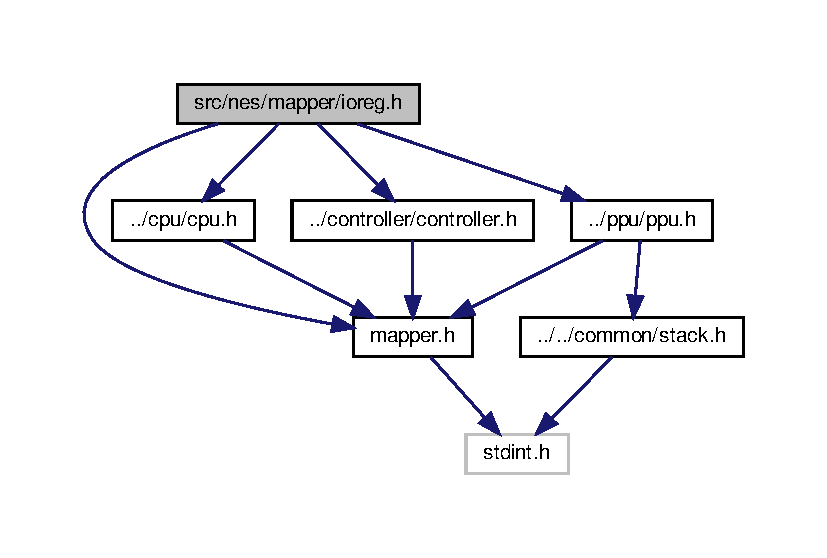
\includegraphics[width=350pt]{ioreg_8h__incl}
\end{center}
\end{figure}
This graph shows which files directly or indirectly include this file\+:\nopagebreak
\begin{figure}[H]
\begin{center}
\leavevmode
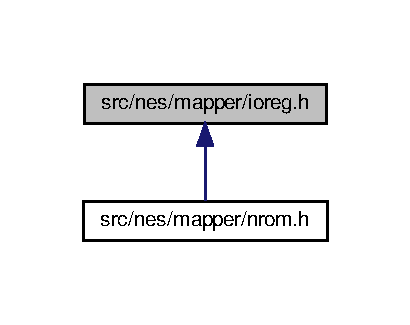
\includegraphics[width=197pt]{ioreg_8h__dep__incl}
\end{center}
\end{figure}
\subsection*{Data Structures}
\begin{DoxyCompactItemize}
\item 
struct \hyperlink{struct_i_o_reg}{I\+O\+Reg}
\begin{DoxyCompactList}\small\item\em Register use to communicate with \hyperlink{struct_p_p_u}{P\+PU}, A\+PU and joystick. \end{DoxyCompactList}\end{DoxyCompactItemize}
\subsection*{Enumerations}
\begin{DoxyCompactItemize}
\item 
enum \hyperlink{ioreg_8h_ab8d3ca34dd6f6dcfa2184a88ea429bd0}{Acknowledge} \{ \hyperlink{ioreg_8h_ab8d3ca34dd6f6dcfa2184a88ea429bd0a5290bc211f15f412b006ffd706c1e634}{A\+C\+\_\+\+NO} = 0, 
\hyperlink{ioreg_8h_ab8d3ca34dd6f6dcfa2184a88ea429bd0a0bed031223ee349ca0a515fe19c547f0}{A\+C\+\_\+\+RD} = 16, 
\hyperlink{ioreg_8h_ab8d3ca34dd6f6dcfa2184a88ea429bd0ab4abb52ddbcc6d8ec2d809b6282b8bd1}{A\+C\+\_\+\+WR} = 32
 \}\begin{DoxyCompactList}\small\item\em Type of access. \end{DoxyCompactList}
\item 
\mbox{\Hypertarget{ioreg_8h_a30a71329f3a6fcf7e2c5d52525002cc3}\label{ioreg_8h_a30a71329f3a6fcf7e2c5d52525002cc3}} 
enum \hyperlink{ioreg_8h_a30a71329f3a6fcf7e2c5d52525002cc3}{Bank1\+Register} \{ \newline
{\bfseries P\+P\+U\+C\+T\+RL} = 0, 
{\bfseries P\+P\+U\+M\+A\+SK}, 
{\bfseries P\+P\+U\+S\+T\+A\+T\+US}, 
{\bfseries O\+A\+M\+A\+D\+DR}, 
\newline
{\bfseries O\+A\+M\+D\+A\+TA}, 
{\bfseries P\+P\+U\+S\+C\+R\+O\+LL}, 
{\bfseries P\+P\+U\+A\+D\+DR}, 
{\bfseries P\+P\+U\+D\+A\+TA}
 \}\begin{DoxyCompactList}\small\item\em Mnemonic for Bank 1 registers. \end{DoxyCompactList}
\item 
\mbox{\Hypertarget{ioreg_8h_a9657e26cc559be8a7adeb2aaea6a0870}\label{ioreg_8h_a9657e26cc559be8a7adeb2aaea6a0870}} 
enum \hyperlink{ioreg_8h_a9657e26cc559be8a7adeb2aaea6a0870}{Bank2\+Register} \{ \newline
{\bfseries S\+Q1\+\_\+\+V\+OL} = 0, 
{\bfseries S\+Q1\+\_\+\+S\+W\+E\+EP}, 
{\bfseries S\+Q1\+\_\+\+LO}, 
{\bfseries S\+Q1\+\_\+\+HI}, 
\newline
{\bfseries S\+Q2\+\_\+\+V\+OL}, 
{\bfseries S\+Q2\+\_\+\+S\+W\+E\+EP}, 
{\bfseries S\+Q2\+\_\+\+LO}, 
{\bfseries S\+Q2\+\_\+\+HI}, 
\newline
{\bfseries T\+R\+I\+\_\+\+L\+I\+N\+E\+AR}, 
{\bfseries B\+A\+N\+K2\+\_\+\+U\+N\+U\+S\+E\+D1}, 
{\bfseries T\+R\+I\+\_\+\+LO}, 
{\bfseries T\+R\+I\+\_\+\+HI}, 
\newline
{\bfseries N\+O\+I\+S\+E\+\_\+\+V\+OL}, 
{\bfseries B\+A\+N\+K2\+\_\+\+U\+N\+U\+S\+E\+D2}, 
{\bfseries N\+O\+I\+S\+E\+\_\+\+LO}, 
{\bfseries N\+O\+I\+S\+E\+\_\+\+HI}, 
\newline
{\bfseries D\+M\+C\+\_\+\+F\+R\+EQ}, 
{\bfseries D\+M\+C\+\_\+\+R\+AW}, 
{\bfseries D\+M\+C\+\_\+\+S\+T\+A\+RT}, 
{\bfseries D\+M\+C\+\_\+\+L\+EN}, 
\newline
{\bfseries O\+A\+M\+D\+MA}, 
{\bfseries S\+N\+D\+\_\+\+C\+HN}, 
{\bfseries J\+O\+Y1}, 
{\bfseries J\+O\+Y2}
 \}\begin{DoxyCompactList}\small\item\em Mnemonic for Bank 2 registers. \end{DoxyCompactList}
\end{DoxyCompactItemize}
\subsection*{Functions}
\begin{DoxyCompactItemize}
\item 
\hyperlink{struct_i_o_reg}{I\+O\+Reg} $\ast$ \hyperlink{ioreg_8h_a8250f90a802b6c70eb0bb3623df8171d}{I\+O\+Reg\+\_\+\+Create} (void)
\begin{DoxyCompactList}\small\item\em Instanciation of \hyperlink{struct_i_o_reg}{I\+O\+Reg}. \end{DoxyCompactList}\item 
uint8\+\_\+t \hyperlink{ioreg_8h_a050b34fa7b8346d8ea93be49a00beef0}{I\+O\+Reg\+\_\+\+Connect} (\hyperlink{struct_i_o_reg}{I\+O\+Reg} $\ast$self, \hyperlink{struct_c_p_u}{C\+PU} $\ast$cpu, \hyperlink{struct_p_p_u}{P\+PU} $\ast$ppu, \hyperlink{struct_controller}{Controller} $\ast$ctrl)
\begin{DoxyCompactList}\small\item\em I\+O\+Reg\+\_\+\+Connect. \end{DoxyCompactList}\item 
uint8\+\_\+t $\ast$ \hyperlink{ioreg_8h_a16528b558e5d5d79b739fdf66993b4d6}{I\+O\+Reg\+\_\+\+Get} (\hyperlink{struct_i_o_reg}{I\+O\+Reg} $\ast$self, uint8\+\_\+t access\+Type, uint16\+\_\+t address)
\begin{DoxyCompactList}\small\item\em Get pointer to access IO register. \end{DoxyCompactList}\item 
uint8\+\_\+t \hyperlink{ioreg_8h_af56c6a4168ccbc88da6a5d1984133c0b}{I\+O\+Reg\+\_\+\+Ack} (\hyperlink{struct_i_o_reg}{I\+O\+Reg} $\ast$self, uint16\+\_\+t address)
\begin{DoxyCompactList}\small\item\em Check if the selected IO register was accessed before and acknowledge it. \end{DoxyCompactList}\item 
void \hyperlink{ioreg_8h_a0d350409c35be2798ddd95b017a4ea9c}{I\+O\+Reg\+\_\+\+Destroy} (\hyperlink{struct_i_o_reg}{I\+O\+Reg} $\ast$self)
\begin{DoxyCompactList}\small\item\em Free instance of \hyperlink{struct_i_o_reg}{I\+O\+Reg}. \end{DoxyCompactList}\item 
\hyperlink{struct_i_o_reg}{I\+O\+Reg} $\ast$ \hyperlink{ioreg_8h_a196fef356357d5def1eebe5a1438f567}{I\+O\+Reg\+\_\+\+Extract} (\hyperlink{struct_mapper}{Mapper} $\ast$mapper)
\begin{DoxyCompactList}\small\item\em I\+O\+Reg\+\_\+\+Extract. \end{DoxyCompactList}\end{DoxyCompactItemize}


\subsection{Detailed Description}
header file of \hyperlink{struct_i_o_reg}{I\+O\+Reg} module 

\begin{DoxyAuthor}{Author}
Dylan Gageot 
\end{DoxyAuthor}
\begin{DoxyVersion}{Version}
1.\+0 
\end{DoxyVersion}
\begin{DoxyDate}{Date}
2019-\/03-\/31 
\end{DoxyDate}


\subsection{Enumeration Type Documentation}
\mbox{\Hypertarget{ioreg_8h_ab8d3ca34dd6f6dcfa2184a88ea429bd0}\label{ioreg_8h_ab8d3ca34dd6f6dcfa2184a88ea429bd0}} 
\index{ioreg.\+h@{ioreg.\+h}!Acknowledge@{Acknowledge}}
\index{Acknowledge@{Acknowledge}!ioreg.\+h@{ioreg.\+h}}
\subsubsection{\texorpdfstring{Acknowledge}{Acknowledge}}
{\footnotesize\ttfamily enum \hyperlink{ioreg_8h_ab8d3ca34dd6f6dcfa2184a88ea429bd0}{Acknowledge}}



Type of access. 

\begin{DoxyEnumFields}{Enumerator}
\raisebox{\heightof{T}}[0pt][0pt]{\index{A\+C\+\_\+\+NO@{A\+C\+\_\+\+NO}!ioreg.\+h@{ioreg.\+h}}\index{ioreg.\+h@{ioreg.\+h}!A\+C\+\_\+\+NO@{A\+C\+\_\+\+NO}}}\mbox{\Hypertarget{ioreg_8h_ab8d3ca34dd6f6dcfa2184a88ea429bd0a5290bc211f15f412b006ffd706c1e634}\label{ioreg_8h_ab8d3ca34dd6f6dcfa2184a88ea429bd0a5290bc211f15f412b006ffd706c1e634}} 
A\+C\+\_\+\+NO&Transparent access \\
\hline

\raisebox{\heightof{T}}[0pt][0pt]{\index{A\+C\+\_\+\+RD@{A\+C\+\_\+\+RD}!ioreg.\+h@{ioreg.\+h}}\index{ioreg.\+h@{ioreg.\+h}!A\+C\+\_\+\+RD@{A\+C\+\_\+\+RD}}}\mbox{\Hypertarget{ioreg_8h_ab8d3ca34dd6f6dcfa2184a88ea429bd0a0bed031223ee349ca0a515fe19c547f0}\label{ioreg_8h_ab8d3ca34dd6f6dcfa2184a88ea429bd0a0bed031223ee349ca0a515fe19c547f0}} 
A\+C\+\_\+\+RD&Set register as read \\
\hline

\raisebox{\heightof{T}}[0pt][0pt]{\index{A\+C\+\_\+\+WR@{A\+C\+\_\+\+WR}!ioreg.\+h@{ioreg.\+h}}\index{ioreg.\+h@{ioreg.\+h}!A\+C\+\_\+\+WR@{A\+C\+\_\+\+WR}}}\mbox{\Hypertarget{ioreg_8h_ab8d3ca34dd6f6dcfa2184a88ea429bd0ab4abb52ddbcc6d8ec2d809b6282b8bd1}\label{ioreg_8h_ab8d3ca34dd6f6dcfa2184a88ea429bd0ab4abb52ddbcc6d8ec2d809b6282b8bd1}} 
A\+C\+\_\+\+WR&Set register as written \\
\hline

\end{DoxyEnumFields}


\subsection{Function Documentation}
\mbox{\Hypertarget{ioreg_8h_af56c6a4168ccbc88da6a5d1984133c0b}\label{ioreg_8h_af56c6a4168ccbc88da6a5d1984133c0b}} 
\index{ioreg.\+h@{ioreg.\+h}!I\+O\+Reg\+\_\+\+Ack@{I\+O\+Reg\+\_\+\+Ack}}
\index{I\+O\+Reg\+\_\+\+Ack@{I\+O\+Reg\+\_\+\+Ack}!ioreg.\+h@{ioreg.\+h}}
\subsubsection{\texorpdfstring{I\+O\+Reg\+\_\+\+Ack()}{IOReg\_Ack()}}
{\footnotesize\ttfamily uint8\+\_\+t I\+O\+Reg\+\_\+\+Ack (\begin{DoxyParamCaption}\item[{\hyperlink{struct_i_o_reg}{I\+O\+Reg} $\ast$}]{self,  }\item[{uint16\+\_\+t}]{address }\end{DoxyParamCaption})}



Check if the selected IO register was accessed before and acknowledge it. 


\begin{DoxyParams}{Parameters}
{\em self} & instance of \hyperlink{struct_i_o_reg}{I\+O\+Reg} \\
\hline
{\em address} & address to check\\
\hline
\end{DoxyParams}
\begin{DoxyReturn}{Returns}
1 if accessed, 0 otherwise 
\end{DoxyReturn}
\mbox{\Hypertarget{ioreg_8h_a050b34fa7b8346d8ea93be49a00beef0}\label{ioreg_8h_a050b34fa7b8346d8ea93be49a00beef0}} 
\index{ioreg.\+h@{ioreg.\+h}!I\+O\+Reg\+\_\+\+Connect@{I\+O\+Reg\+\_\+\+Connect}}
\index{I\+O\+Reg\+\_\+\+Connect@{I\+O\+Reg\+\_\+\+Connect}!ioreg.\+h@{ioreg.\+h}}
\subsubsection{\texorpdfstring{I\+O\+Reg\+\_\+\+Connect()}{IOReg\_Connect()}}
{\footnotesize\ttfamily uint8\+\_\+t I\+O\+Reg\+\_\+\+Connect (\begin{DoxyParamCaption}\item[{\hyperlink{struct_i_o_reg}{I\+O\+Reg} $\ast$}]{self,  }\item[{\hyperlink{struct_c_p_u}{C\+PU} $\ast$}]{cpu,  }\item[{\hyperlink{struct_p_p_u}{P\+PU} $\ast$}]{ppu,  }\item[{\hyperlink{struct_controller}{Controller} $\ast$}]{ctrl }\end{DoxyParamCaption})}



I\+O\+Reg\+\_\+\+Connect. 


\begin{DoxyParams}{Parameters}
{\em self} & instance of \hyperlink{struct_i_o_reg}{I\+O\+Reg} \\
\hline
{\em cpu} & instance of \hyperlink{struct_c_p_u}{C\+PU} \\
\hline
{\em ppu} & instance of \hyperlink{struct_p_p_u}{P\+PU} \\
\hline
{\em ctrl} & instance of \hyperlink{struct_controller}{Controller}\\
\hline
\end{DoxyParams}
\begin{DoxyReturn}{Returns}
E\+X\+I\+T\+\_\+\+S\+U\+C\+C\+E\+SS if succeed, E\+X\+I\+T\+\_\+\+F\+A\+I\+L\+U\+RE otherwise 
\end{DoxyReturn}
\mbox{\Hypertarget{ioreg_8h_a8250f90a802b6c70eb0bb3623df8171d}\label{ioreg_8h_a8250f90a802b6c70eb0bb3623df8171d}} 
\index{ioreg.\+h@{ioreg.\+h}!I\+O\+Reg\+\_\+\+Create@{I\+O\+Reg\+\_\+\+Create}}
\index{I\+O\+Reg\+\_\+\+Create@{I\+O\+Reg\+\_\+\+Create}!ioreg.\+h@{ioreg.\+h}}
\subsubsection{\texorpdfstring{I\+O\+Reg\+\_\+\+Create()}{IOReg\_Create()}}
{\footnotesize\ttfamily \hyperlink{struct_i_o_reg}{I\+O\+Reg}$\ast$ I\+O\+Reg\+\_\+\+Create (\begin{DoxyParamCaption}\item[{void}]{ }\end{DoxyParamCaption})}



Instanciation of \hyperlink{struct_i_o_reg}{I\+O\+Reg}. 

\begin{DoxyReturn}{Returns}
instance of \hyperlink{struct_i_o_reg}{I\+O\+Reg} if succeed 
\end{DoxyReturn}
\mbox{\Hypertarget{ioreg_8h_a0d350409c35be2798ddd95b017a4ea9c}\label{ioreg_8h_a0d350409c35be2798ddd95b017a4ea9c}} 
\index{ioreg.\+h@{ioreg.\+h}!I\+O\+Reg\+\_\+\+Destroy@{I\+O\+Reg\+\_\+\+Destroy}}
\index{I\+O\+Reg\+\_\+\+Destroy@{I\+O\+Reg\+\_\+\+Destroy}!ioreg.\+h@{ioreg.\+h}}
\subsubsection{\texorpdfstring{I\+O\+Reg\+\_\+\+Destroy()}{IOReg\_Destroy()}}
{\footnotesize\ttfamily void I\+O\+Reg\+\_\+\+Destroy (\begin{DoxyParamCaption}\item[{\hyperlink{struct_i_o_reg}{I\+O\+Reg} $\ast$}]{self }\end{DoxyParamCaption})}



Free instance of \hyperlink{struct_i_o_reg}{I\+O\+Reg}. 


\begin{DoxyParams}{Parameters}
{\em self} & instance of \hyperlink{struct_i_o_reg}{I\+O\+Reg} \\
\hline
\end{DoxyParams}
\mbox{\Hypertarget{ioreg_8h_a196fef356357d5def1eebe5a1438f567}\label{ioreg_8h_a196fef356357d5def1eebe5a1438f567}} 
\index{ioreg.\+h@{ioreg.\+h}!I\+O\+Reg\+\_\+\+Extract@{I\+O\+Reg\+\_\+\+Extract}}
\index{I\+O\+Reg\+\_\+\+Extract@{I\+O\+Reg\+\_\+\+Extract}!ioreg.\+h@{ioreg.\+h}}
\subsubsection{\texorpdfstring{I\+O\+Reg\+\_\+\+Extract()}{IOReg\_Extract()}}
{\footnotesize\ttfamily \hyperlink{struct_i_o_reg}{I\+O\+Reg}$\ast$ I\+O\+Reg\+\_\+\+Extract (\begin{DoxyParamCaption}\item[{\hyperlink{struct_mapper}{Mapper} $\ast$}]{mapper }\end{DoxyParamCaption})}



I\+O\+Reg\+\_\+\+Extract. 


\begin{DoxyParams}{Parameters}
{\em mapper} & instance of \hyperlink{struct_mapper}{Mapper}\\
\hline
\end{DoxyParams}
\begin{DoxyReturn}{Returns}
instance of \hyperlink{struct_i_o_reg}{I\+O\+Reg} 
\end{DoxyReturn}
\mbox{\Hypertarget{ioreg_8h_a16528b558e5d5d79b739fdf66993b4d6}\label{ioreg_8h_a16528b558e5d5d79b739fdf66993b4d6}} 
\index{ioreg.\+h@{ioreg.\+h}!I\+O\+Reg\+\_\+\+Get@{I\+O\+Reg\+\_\+\+Get}}
\index{I\+O\+Reg\+\_\+\+Get@{I\+O\+Reg\+\_\+\+Get}!ioreg.\+h@{ioreg.\+h}}
\subsubsection{\texorpdfstring{I\+O\+Reg\+\_\+\+Get()}{IOReg\_Get()}}
{\footnotesize\ttfamily uint8\+\_\+t$\ast$ I\+O\+Reg\+\_\+\+Get (\begin{DoxyParamCaption}\item[{\hyperlink{struct_i_o_reg}{I\+O\+Reg} $\ast$}]{self,  }\item[{uint8\+\_\+t}]{access\+Type,  }\item[{uint16\+\_\+t}]{address }\end{DoxyParamCaption})}



Get pointer to access IO register. 


\begin{DoxyParams}{Parameters}
{\em self} & instance of \hyperlink{struct_i_o_reg}{I\+O\+Reg} \\
\hline
{\em access\+Type} & which address type and which type of access (rd,wr) ? \\
\hline
{\em address} & address to access\\
\hline
\end{DoxyParams}
\begin{DoxyReturn}{Returns}
pointer to selected IO register 
\end{DoxyReturn}

\hypertarget{mapper_8h}{}\section{src/nes/mapper/mapper.h File Reference}
\label{mapper_8h}\index{src/nes/mapper/mapper.\+h@{src/nes/mapper/mapper.\+h}}


header file of \hyperlink{struct_mapper}{Mapper} module  


{\ttfamily \#include \char`\"{}stdint.\+h\char`\"{}}\newline
Include dependency graph for mapper.\+h\+:\nopagebreak
\begin{figure}[H]
\begin{center}
\leavevmode
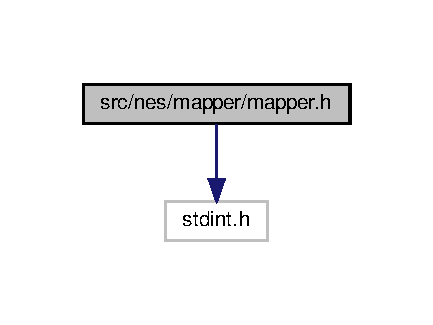
\includegraphics[width=208pt]{mapper_8h__incl}
\end{center}
\end{figure}
This graph shows which files directly or indirectly include this file\+:\nopagebreak
\begin{figure}[H]
\begin{center}
\leavevmode
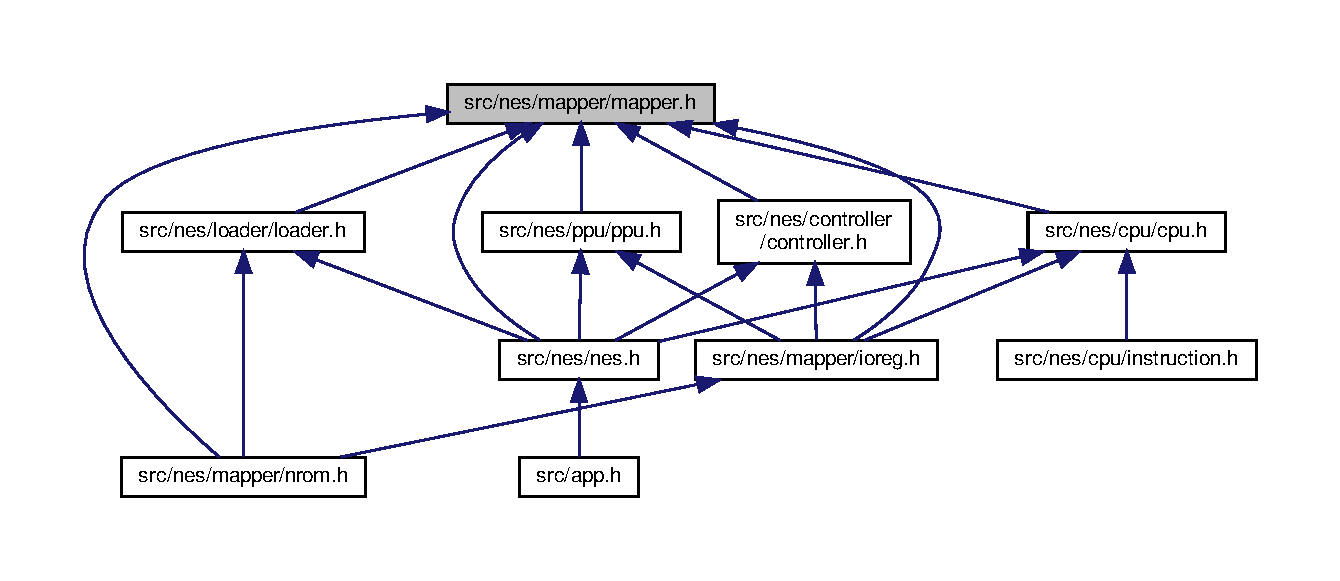
\includegraphics[width=350pt]{mapper_8h__dep__incl}
\end{center}
\end{figure}
\subsection*{Data Structures}
\begin{DoxyCompactItemize}
\item 
struct \hyperlink{struct_mapper}{Mapper}
\begin{DoxyCompactList}\small\item\em Generic structure to hold mapper. \end{DoxyCompactList}\end{DoxyCompactItemize}
\subsection*{Enumerations}
\begin{DoxyCompactItemize}
\item 
enum \hyperlink{mapper_8h_a9387b3dd9068d2012b3fb9dc44191672}{Address\+Space} \{ \hyperlink{mapper_8h_a9387b3dd9068d2012b3fb9dc44191672af8121c0f8df681863b2381f6ec599041}{A\+S\+\_\+\+C\+PU} = 0, 
\hyperlink{mapper_8h_a9387b3dd9068d2012b3fb9dc44191672a4758dfa9ec095b60d0f3fa616c798480}{A\+S\+\_\+\+P\+PU}, 
\hyperlink{mapper_8h_a9387b3dd9068d2012b3fb9dc44191672a9fa8fba91d4a2b04d6a0288882950e45}{A\+S\+\_\+\+L\+DR}
 \}\begin{DoxyCompactList}\small\item\em Use to specify to the mapper in which address space we want to retrieve the data. \end{DoxyCompactList}
\item 
enum \hyperlink{mapper_8h_a01f18757791d134ebfcac29738a70f68}{Loader\+Data} \{ \hyperlink{mapper_8h_a01f18757791d134ebfcac29738a70f68a4de1befec88b1dac8e0a905707cdb56c}{L\+D\+R\+\_\+\+P\+RG} = 0, 
\hyperlink{mapper_8h_a01f18757791d134ebfcac29738a70f68a6c90ffd14690523970700d61e780dab8}{L\+D\+R\+\_\+\+C\+HR}, 
\hyperlink{mapper_8h_a01f18757791d134ebfcac29738a70f68aa9a0e3cb5dda5a858d4e24a998b0d85e}{L\+D\+R\+\_\+\+I\+OR}
 \}\begin{DoxyCompactList}\small\item\em Use to get pointer to P\+R\+G\+R\+OM and C\+H\+R\+R\+OM. \end{DoxyCompactList}
\end{DoxyCompactItemize}
\subsection*{Functions}
\begin{DoxyCompactItemize}
\item 
\hyperlink{struct_mapper}{Mapper} $\ast$ \hyperlink{mapper_8h_ab7efcdf3e7b12eeed777c66551d056c6}{Mapper\+\_\+\+Create} (void $\ast$($\ast$get)(void $\ast$, uint8\+\_\+t, uint16\+\_\+t), void($\ast$destroyer)(void $\ast$), uint8\+\_\+t($\ast$ack)(void $\ast$, uint16\+\_\+t), void $\ast$mapper\+Data)
\begin{DoxyCompactList}\small\item\em Create instance of mapper from callback and data of specific mapper. \end{DoxyCompactList}\item 
void \hyperlink{mapper_8h_a808b5d82dd209d051933e060dda17469}{Mapper\+\_\+\+Destroy} (\hyperlink{struct_mapper}{Mapper} $\ast$self)
\begin{DoxyCompactList}\small\item\em Destroy instance of \hyperlink{struct_mapper}{Mapper}. \end{DoxyCompactList}\item 
uint8\+\_\+t $\ast$ \hyperlink{mapper_8h_a4eb170906c0a22a554aadd5d9bc2acb9}{Mapper\+\_\+\+Get} (\hyperlink{struct_mapper}{Mapper} $\ast$self, uint8\+\_\+t space, uint16\+\_\+t address)
\begin{DoxyCompactList}\small\item\em Get pointer from memory for a specific address. \end{DoxyCompactList}\item 
uint8\+\_\+t \hyperlink{mapper_8h_a57991ddbdc6a0b643ca8101be19ca26f}{Mapper\+\_\+\+Ack} (\hyperlink{struct_mapper}{Mapper} $\ast$self, uint16\+\_\+t address)
\begin{DoxyCompactList}\small\item\em Ask for the last type of access at a register and aknowledge it. \end{DoxyCompactList}\end{DoxyCompactItemize}


\subsection{Detailed Description}
header file of \hyperlink{struct_mapper}{Mapper} module 

\begin{DoxyAuthor}{Author}
Dylan Gageot 
\end{DoxyAuthor}
\begin{DoxyVersion}{Version}
1.\+0 
\end{DoxyVersion}
\begin{DoxyDate}{Date}
2019-\/02-\/20 
\end{DoxyDate}


\subsection{Enumeration Type Documentation}
\mbox{\Hypertarget{mapper_8h_a9387b3dd9068d2012b3fb9dc44191672}\label{mapper_8h_a9387b3dd9068d2012b3fb9dc44191672}} 
\index{mapper.\+h@{mapper.\+h}!Address\+Space@{Address\+Space}}
\index{Address\+Space@{Address\+Space}!mapper.\+h@{mapper.\+h}}
\subsubsection{\texorpdfstring{Address\+Space}{AddressSpace}}
{\footnotesize\ttfamily enum \hyperlink{mapper_8h_a9387b3dd9068d2012b3fb9dc44191672}{Address\+Space}}



Use to specify to the mapper in which address space we want to retrieve the data. 

\begin{DoxyEnumFields}{Enumerator}
\raisebox{\heightof{T}}[0pt][0pt]{\index{A\+S\+\_\+\+C\+PU@{A\+S\+\_\+\+C\+PU}!mapper.\+h@{mapper.\+h}}\index{mapper.\+h@{mapper.\+h}!A\+S\+\_\+\+C\+PU@{A\+S\+\_\+\+C\+PU}}}\mbox{\Hypertarget{mapper_8h_a9387b3dd9068d2012b3fb9dc44191672af8121c0f8df681863b2381f6ec599041}\label{mapper_8h_a9387b3dd9068d2012b3fb9dc44191672af8121c0f8df681863b2381f6ec599041}} 
A\+S\+\_\+\+C\+PU&\hyperlink{struct_c_p_u}{C\+PU} address space \\
\hline

\raisebox{\heightof{T}}[0pt][0pt]{\index{A\+S\+\_\+\+P\+PU@{A\+S\+\_\+\+P\+PU}!mapper.\+h@{mapper.\+h}}\index{mapper.\+h@{mapper.\+h}!A\+S\+\_\+\+P\+PU@{A\+S\+\_\+\+P\+PU}}}\mbox{\Hypertarget{mapper_8h_a9387b3dd9068d2012b3fb9dc44191672a4758dfa9ec095b60d0f3fa616c798480}\label{mapper_8h_a9387b3dd9068d2012b3fb9dc44191672a4758dfa9ec095b60d0f3fa616c798480}} 
A\+S\+\_\+\+P\+PU&\hyperlink{struct_p_p_u}{P\+PU} addrsss space \\
\hline

\raisebox{\heightof{T}}[0pt][0pt]{\index{A\+S\+\_\+\+L\+DR@{A\+S\+\_\+\+L\+DR}!mapper.\+h@{mapper.\+h}}\index{mapper.\+h@{mapper.\+h}!A\+S\+\_\+\+L\+DR@{A\+S\+\_\+\+L\+DR}}}\mbox{\Hypertarget{mapper_8h_a9387b3dd9068d2012b3fb9dc44191672a9fa8fba91d4a2b04d6a0288882950e45}\label{mapper_8h_a9387b3dd9068d2012b3fb9dc44191672a9fa8fba91d4a2b04d6a0288882950e45}} 
A\+S\+\_\+\+L\+DR&Loader special access \\
\hline

\end{DoxyEnumFields}
\mbox{\Hypertarget{mapper_8h_a01f18757791d134ebfcac29738a70f68}\label{mapper_8h_a01f18757791d134ebfcac29738a70f68}} 
\index{mapper.\+h@{mapper.\+h}!Loader\+Data@{Loader\+Data}}
\index{Loader\+Data@{Loader\+Data}!mapper.\+h@{mapper.\+h}}
\subsubsection{\texorpdfstring{Loader\+Data}{LoaderData}}
{\footnotesize\ttfamily enum \hyperlink{mapper_8h_a01f18757791d134ebfcac29738a70f68}{Loader\+Data}}



Use to get pointer to P\+R\+G\+R\+OM and C\+H\+R\+R\+OM. 

\begin{DoxyEnumFields}{Enumerator}
\raisebox{\heightof{T}}[0pt][0pt]{\index{L\+D\+R\+\_\+\+P\+RG@{L\+D\+R\+\_\+\+P\+RG}!mapper.\+h@{mapper.\+h}}\index{mapper.\+h@{mapper.\+h}!L\+D\+R\+\_\+\+P\+RG@{L\+D\+R\+\_\+\+P\+RG}}}\mbox{\Hypertarget{mapper_8h_a01f18757791d134ebfcac29738a70f68a4de1befec88b1dac8e0a905707cdb56c}\label{mapper_8h_a01f18757791d134ebfcac29738a70f68a4de1befec88b1dac8e0a905707cdb56c}} 
L\+D\+R\+\_\+\+P\+RG&Get pointer for P\+G\+R-\/\+R\+OM \\
\hline

\raisebox{\heightof{T}}[0pt][0pt]{\index{L\+D\+R\+\_\+\+C\+HR@{L\+D\+R\+\_\+\+C\+HR}!mapper.\+h@{mapper.\+h}}\index{mapper.\+h@{mapper.\+h}!L\+D\+R\+\_\+\+C\+HR@{L\+D\+R\+\_\+\+C\+HR}}}\mbox{\Hypertarget{mapper_8h_a01f18757791d134ebfcac29738a70f68a6c90ffd14690523970700d61e780dab8}\label{mapper_8h_a01f18757791d134ebfcac29738a70f68a6c90ffd14690523970700d61e780dab8}} 
L\+D\+R\+\_\+\+C\+HR&Get pointer for C\+HR \\
\hline

\raisebox{\heightof{T}}[0pt][0pt]{\index{L\+D\+R\+\_\+\+I\+OR@{L\+D\+R\+\_\+\+I\+OR}!mapper.\+h@{mapper.\+h}}\index{mapper.\+h@{mapper.\+h}!L\+D\+R\+\_\+\+I\+OR@{L\+D\+R\+\_\+\+I\+OR}}}\mbox{\Hypertarget{mapper_8h_a01f18757791d134ebfcac29738a70f68aa9a0e3cb5dda5a858d4e24a998b0d85e}\label{mapper_8h_a01f18757791d134ebfcac29738a70f68aa9a0e3cb5dda5a858d4e24a998b0d85e}} 
L\+D\+R\+\_\+\+I\+OR&Get pointer for \hyperlink{struct_i_o_reg}{I\+O\+Reg} \\
\hline

\end{DoxyEnumFields}


\subsection{Function Documentation}
\mbox{\Hypertarget{mapper_8h_a57991ddbdc6a0b643ca8101be19ca26f}\label{mapper_8h_a57991ddbdc6a0b643ca8101be19ca26f}} 
\index{mapper.\+h@{mapper.\+h}!Mapper\+\_\+\+Ack@{Mapper\+\_\+\+Ack}}
\index{Mapper\+\_\+\+Ack@{Mapper\+\_\+\+Ack}!mapper.\+h@{mapper.\+h}}
\subsubsection{\texorpdfstring{Mapper\+\_\+\+Ack()}{Mapper\_Ack()}}
{\footnotesize\ttfamily uint8\+\_\+t Mapper\+\_\+\+Ack (\begin{DoxyParamCaption}\item[{\hyperlink{struct_mapper}{Mapper} $\ast$}]{self,  }\item[{uint16\+\_\+t}]{address }\end{DoxyParamCaption})}



Ask for the last type of access at a register and aknowledge it. 


\begin{DoxyParams}{Parameters}
{\em self} & instance of \hyperlink{struct_mapper}{Mapper} \\
\hline
{\em address} & address to get access information from\\
\hline
\end{DoxyParams}
\begin{DoxyReturn}{Returns}
1 if address accesed before, 0 otherwise 
\end{DoxyReturn}
\mbox{\Hypertarget{mapper_8h_ab7efcdf3e7b12eeed777c66551d056c6}\label{mapper_8h_ab7efcdf3e7b12eeed777c66551d056c6}} 
\index{mapper.\+h@{mapper.\+h}!Mapper\+\_\+\+Create@{Mapper\+\_\+\+Create}}
\index{Mapper\+\_\+\+Create@{Mapper\+\_\+\+Create}!mapper.\+h@{mapper.\+h}}
\subsubsection{\texorpdfstring{Mapper\+\_\+\+Create()}{Mapper\_Create()}}
{\footnotesize\ttfamily \hyperlink{struct_mapper}{Mapper}$\ast$ Mapper\+\_\+\+Create (\begin{DoxyParamCaption}\item[{void $\ast$($\ast$)(void $\ast$, uint8\+\_\+t, uint16\+\_\+t)}]{get,  }\item[{void($\ast$)(void $\ast$)}]{destroyer,  }\item[{uint8\+\_\+t($\ast$)(void $\ast$, uint16\+\_\+t)}]{ack,  }\item[{void $\ast$}]{mapper\+Data }\end{DoxyParamCaption})}



Create instance of mapper from callback and data of specific mapper. 


\begin{DoxyParams}{Parameters}
{\em get} & Get callback \\
\hline
{\em destroyer} & Destroyer callback \\
\hline
{\em ack} & Acknowledge callback \\
\hline
{\em mapper\+Data} & \hyperlink{struct_mapper}{Mapper} data\\
\hline
\end{DoxyParams}
\begin{DoxyReturn}{Returns}
instance of \hyperlink{struct_mapper}{Mapper} 
\end{DoxyReturn}
\mbox{\Hypertarget{mapper_8h_a808b5d82dd209d051933e060dda17469}\label{mapper_8h_a808b5d82dd209d051933e060dda17469}} 
\index{mapper.\+h@{mapper.\+h}!Mapper\+\_\+\+Destroy@{Mapper\+\_\+\+Destroy}}
\index{Mapper\+\_\+\+Destroy@{Mapper\+\_\+\+Destroy}!mapper.\+h@{mapper.\+h}}
\subsubsection{\texorpdfstring{Mapper\+\_\+\+Destroy()}{Mapper\_Destroy()}}
{\footnotesize\ttfamily void Mapper\+\_\+\+Destroy (\begin{DoxyParamCaption}\item[{\hyperlink{struct_mapper}{Mapper} $\ast$}]{self }\end{DoxyParamCaption})}



Destroy instance of \hyperlink{struct_mapper}{Mapper}. 


\begin{DoxyParams}{Parameters}
{\em self} & free \hyperlink{struct_mapper}{Mapper} allocation \\
\hline
\end{DoxyParams}
\mbox{\Hypertarget{mapper_8h_a4eb170906c0a22a554aadd5d9bc2acb9}\label{mapper_8h_a4eb170906c0a22a554aadd5d9bc2acb9}} 
\index{mapper.\+h@{mapper.\+h}!Mapper\+\_\+\+Get@{Mapper\+\_\+\+Get}}
\index{Mapper\+\_\+\+Get@{Mapper\+\_\+\+Get}!mapper.\+h@{mapper.\+h}}
\subsubsection{\texorpdfstring{Mapper\+\_\+\+Get()}{Mapper\_Get()}}
{\footnotesize\ttfamily uint8\+\_\+t$\ast$ Mapper\+\_\+\+Get (\begin{DoxyParamCaption}\item[{\hyperlink{struct_mapper}{Mapper} $\ast$}]{self,  }\item[{uint8\+\_\+t}]{space,  }\item[{uint16\+\_\+t}]{address }\end{DoxyParamCaption})}



Get pointer from memory for a specific address. 


\begin{DoxyParams}{Parameters}
{\em self} & instance of \hyperlink{struct_mapper}{Mapper} \\
\hline
{\em space} & in which address space to look and with type of access \\
\hline
{\em address} & address to get data from\\
\hline
\end{DoxyParams}
\begin{DoxyReturn}{Returns}
pointer of pointed data 
\end{DoxyReturn}

\hypertarget{nrom_8h}{}\section{src/nes/mapper/nrom.h File Reference}
\label{nrom_8h}\index{src/nes/mapper/nrom.\+h@{src/nes/mapper/nrom.\+h}}


header file of N\+R\+OM mapper module  


{\ttfamily \#include \char`\"{}mapper.\+h\char`\"{}}\newline
{\ttfamily \#include \char`\"{}ioreg.\+h\char`\"{}}\newline
{\ttfamily \#include \char`\"{}../loader/loader.\+h\char`\"{}}\newline
Include dependency graph for nrom.\+h\+:\nopagebreak
\begin{figure}[H]
\begin{center}
\leavevmode
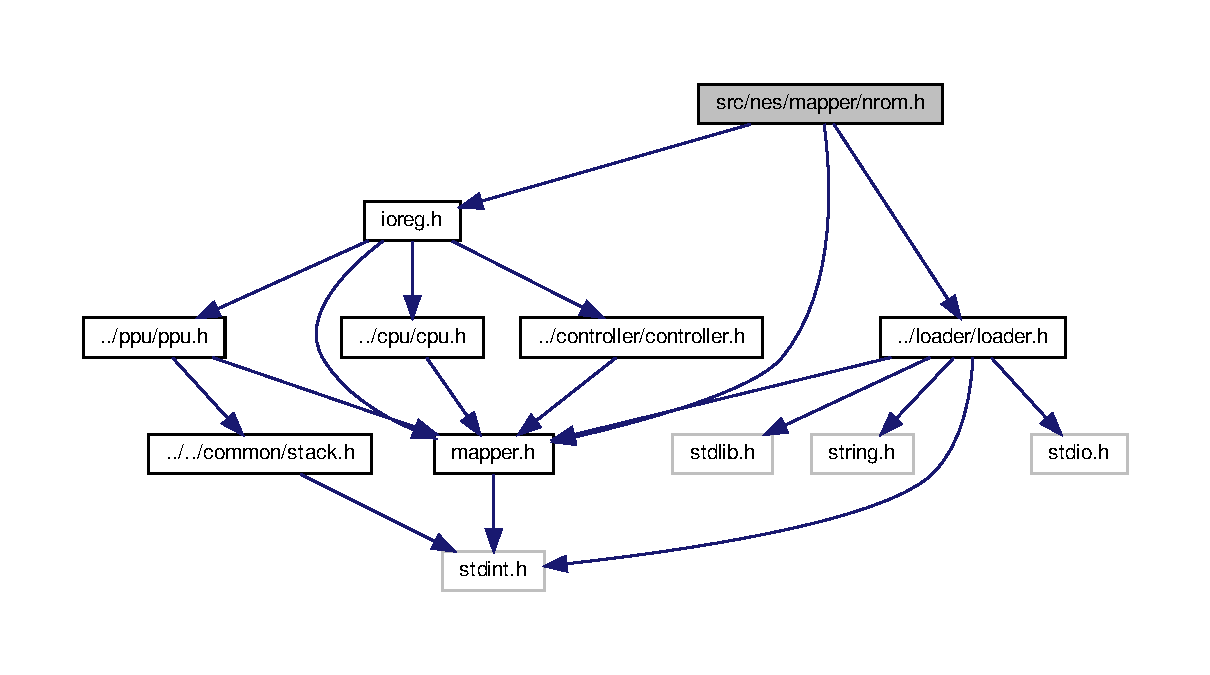
\includegraphics[width=350pt]{nrom_8h__incl}
\end{center}
\end{figure}
\subsection*{Data Structures}
\begin{DoxyCompactItemize}
\item 
struct \hyperlink{struct_map_n_r_o_m___c_p_u}{Map\+N\+R\+O\+M\+\_\+\+C\+PU}
\begin{DoxyCompactList}\small\item\em Memory map of \hyperlink{struct_c_p_u}{C\+PU} when using N\+R\+OM mapper. \end{DoxyCompactList}\item 
struct \hyperlink{struct_map_n_r_o_m___p_p_u}{Map\+N\+R\+O\+M\+\_\+\+P\+PU}
\begin{DoxyCompactList}\small\item\em Memory map of \hyperlink{struct_p_p_u}{P\+PU} when using N\+R\+OM mapper. \end{DoxyCompactList}\item 
struct \hyperlink{struct_map_n_r_o_m}{Map\+N\+R\+OM}
\begin{DoxyCompactList}\small\item\em Memory map used when using N\+R\+OM mapper. \end{DoxyCompactList}\end{DoxyCompactItemize}
\subsection*{Macros}
\begin{DoxyCompactItemize}
\item 
\mbox{\Hypertarget{nrom_8h_a6744e81522354f227e123448e7600f26}\label{nrom_8h_a6744e81522354f227e123448e7600f26}} 
\#define {\bfseries N\+R\+O\+M\+\_\+\+R\+A\+M\+\_\+\+S\+I\+ZE}~2048
\end{DoxyCompactItemize}
\subsection*{Enumerations}
\begin{DoxyCompactItemize}
\item 
\mbox{\Hypertarget{nrom_8h_a6747c71ae48919ee77e55bdc9f7c2953}\label{nrom_8h_a6747c71ae48919ee77e55bdc9f7c2953}} 
enum \hyperlink{nrom_8h_a6747c71ae48919ee77e55bdc9f7c2953}{N\+R\+O\+M\+Size} \{ {\bfseries N\+R\+O\+M\+\_\+32\+K\+IB} = 0, 
{\bfseries N\+R\+O\+M\+\_\+16\+K\+IB}, 
{\bfseries N\+R\+O\+M\+\_\+\+U\+N\+D\+E\+F\+I\+N\+ED}
 \}\begin{DoxyCompactList}\small\item\em Describe if the loaded R\+OM use 16 or 32kiB. \end{DoxyCompactList}
\item 
\mbox{\Hypertarget{nrom_8h_ac78833825c8300ad67c8bfa114053f8b}\label{nrom_8h_ac78833825c8300ad67c8bfa114053f8b}} 
enum \hyperlink{nrom_8h_ac78833825c8300ad67c8bfa114053f8b}{N\+R\+O\+M\+Mirroring} \{ {\bfseries N\+R\+O\+M\+\_\+\+H\+O\+R\+I\+Z\+O\+N\+T\+AL} = 0, 
{\bfseries N\+R\+O\+M\+\_\+\+V\+E\+R\+T\+I\+C\+AL}
 \}\begin{DoxyCompactList}\small\item\em Describe the mirroring mecanism to use. \end{DoxyCompactList}
\end{DoxyCompactItemize}
\subsection*{Functions}
\begin{DoxyCompactItemize}
\item 
\hyperlink{struct_mapper}{Mapper} $\ast$ \hyperlink{nrom_8h_a8099bfb7d89ac70998c53004b6f97ef0}{Map\+N\+R\+O\+M\+\_\+\+Create} (\hyperlink{struct_header}{Header} $\ast$header)
\begin{DoxyCompactList}\small\item\em Allocate memory for N\+R\+OM mapper. \end{DoxyCompactList}\item 
void $\ast$ \hyperlink{nrom_8h_ac335ad14b2bf08cb5af11deb0a3b0583}{Map\+N\+R\+O\+M\+\_\+\+Get} (void $\ast$mapper\+Data, uint8\+\_\+t space, uint16\+\_\+t address)
\begin{DoxyCompactList}\small\item\em Give access to the data addressed in argument. \end{DoxyCompactList}\item 
uint8\+\_\+t \hyperlink{nrom_8h_aa54557799a0346995107e4ea2ef2a7a6}{Map\+N\+R\+O\+M\+\_\+\+Ack} (void $\ast$mapper\+Data, uint16\+\_\+t address)
\begin{DoxyCompactList}\small\item\em Acknowledge \hyperlink{struct_i_o_reg}{I\+O\+Reg} from \hyperlink{struct_map_n_r_o_m}{Map\+N\+R\+OM}. \end{DoxyCompactList}\item 
void \hyperlink{nrom_8h_a387ac6b9eb4e203e7823ae50c2f1120e}{Map\+N\+R\+O\+M\+\_\+\+Destroy} (void $\ast$mapper\+Data)
\begin{DoxyCompactList}\small\item\em Destroy/free the mapper. \end{DoxyCompactList}\end{DoxyCompactItemize}


\subsection{Detailed Description}
header file of N\+R\+OM mapper module 

\begin{DoxyAuthor}{Author}
Dylan Gageot 
\end{DoxyAuthor}
\begin{DoxyVersion}{Version}
1.\+0 
\end{DoxyVersion}
\begin{DoxyDate}{Date}
2019-\/02-\/20 
\end{DoxyDate}


\subsection{Function Documentation}
\mbox{\Hypertarget{nrom_8h_aa54557799a0346995107e4ea2ef2a7a6}\label{nrom_8h_aa54557799a0346995107e4ea2ef2a7a6}} 
\index{nrom.\+h@{nrom.\+h}!Map\+N\+R\+O\+M\+\_\+\+Ack@{Map\+N\+R\+O\+M\+\_\+\+Ack}}
\index{Map\+N\+R\+O\+M\+\_\+\+Ack@{Map\+N\+R\+O\+M\+\_\+\+Ack}!nrom.\+h@{nrom.\+h}}
\subsubsection{\texorpdfstring{Map\+N\+R\+O\+M\+\_\+\+Ack()}{MapNROM\_Ack()}}
{\footnotesize\ttfamily uint8\+\_\+t Map\+N\+R\+O\+M\+\_\+\+Ack (\begin{DoxyParamCaption}\item[{void $\ast$}]{mapper\+Data,  }\item[{uint16\+\_\+t}]{address }\end{DoxyParamCaption})}



Acknowledge \hyperlink{struct_i_o_reg}{I\+O\+Reg} from \hyperlink{struct_map_n_r_o_m}{Map\+N\+R\+OM}. 


\begin{DoxyParams}{Parameters}
{\em mapper\+Data} & instance of \hyperlink{struct_map_n_r_o_m}{Map\+N\+R\+OM} \\
\hline
{\em address} & address to check if it was accessed\\
\hline
\end{DoxyParams}
\begin{DoxyReturn}{Returns}
1 if it was accessed, 0 otherwise 
\end{DoxyReturn}
\mbox{\Hypertarget{nrom_8h_a8099bfb7d89ac70998c53004b6f97ef0}\label{nrom_8h_a8099bfb7d89ac70998c53004b6f97ef0}} 
\index{nrom.\+h@{nrom.\+h}!Map\+N\+R\+O\+M\+\_\+\+Create@{Map\+N\+R\+O\+M\+\_\+\+Create}}
\index{Map\+N\+R\+O\+M\+\_\+\+Create@{Map\+N\+R\+O\+M\+\_\+\+Create}!nrom.\+h@{nrom.\+h}}
\subsubsection{\texorpdfstring{Map\+N\+R\+O\+M\+\_\+\+Create()}{MapNROM\_Create()}}
{\footnotesize\ttfamily \hyperlink{struct_mapper}{Mapper}$\ast$ Map\+N\+R\+O\+M\+\_\+\+Create (\begin{DoxyParamCaption}\item[{\hyperlink{struct_header}{Header} $\ast$}]{header }\end{DoxyParamCaption})}



Allocate memory for N\+R\+OM mapper. 


\begin{DoxyParams}{Parameters}
{\em header} & containing all R\+OM informations\\
\hline
\end{DoxyParams}
\begin{DoxyReturn}{Returns}
pointer to the new allocated mapper 
\end{DoxyReturn}
\mbox{\Hypertarget{nrom_8h_a387ac6b9eb4e203e7823ae50c2f1120e}\label{nrom_8h_a387ac6b9eb4e203e7823ae50c2f1120e}} 
\index{nrom.\+h@{nrom.\+h}!Map\+N\+R\+O\+M\+\_\+\+Destroy@{Map\+N\+R\+O\+M\+\_\+\+Destroy}}
\index{Map\+N\+R\+O\+M\+\_\+\+Destroy@{Map\+N\+R\+O\+M\+\_\+\+Destroy}!nrom.\+h@{nrom.\+h}}
\subsubsection{\texorpdfstring{Map\+N\+R\+O\+M\+\_\+\+Destroy()}{MapNROM\_Destroy()}}
{\footnotesize\ttfamily void Map\+N\+R\+O\+M\+\_\+\+Destroy (\begin{DoxyParamCaption}\item[{void $\ast$}]{mapper\+Data }\end{DoxyParamCaption})}



Destroy/free the mapper. 


\begin{DoxyParams}{Parameters}
{\em mapper\+Data} & Memory map pointer \\
\hline
\end{DoxyParams}
\mbox{\Hypertarget{nrom_8h_ac335ad14b2bf08cb5af11deb0a3b0583}\label{nrom_8h_ac335ad14b2bf08cb5af11deb0a3b0583}} 
\index{nrom.\+h@{nrom.\+h}!Map\+N\+R\+O\+M\+\_\+\+Get@{Map\+N\+R\+O\+M\+\_\+\+Get}}
\index{Map\+N\+R\+O\+M\+\_\+\+Get@{Map\+N\+R\+O\+M\+\_\+\+Get}!nrom.\+h@{nrom.\+h}}
\subsubsection{\texorpdfstring{Map\+N\+R\+O\+M\+\_\+\+Get()}{MapNROM\_Get()}}
{\footnotesize\ttfamily void$\ast$ Map\+N\+R\+O\+M\+\_\+\+Get (\begin{DoxyParamCaption}\item[{void $\ast$}]{mapper\+Data,  }\item[{uint8\+\_\+t}]{space,  }\item[{uint16\+\_\+t}]{address }\end{DoxyParamCaption})}



Give access to the data addressed in argument. 


\begin{DoxyParams}{Parameters}
{\em mapper\+Data} & Memory map pointer \\
\hline
{\em space} & \hyperlink{struct_c_p_u}{C\+PU} or \hyperlink{struct_p_p_u}{P\+PU} address space ? \\
\hline
{\em address} & Address of the data to fetch\\
\hline
\end{DoxyParams}
\begin{DoxyReturn}{Returns}
void$\ast$ pointer of the data addressed 
\end{DoxyReturn}

\hypertarget{nes_8h}{}\section{src/nes/nes.h File Reference}
\label{nes_8h}\index{src/nes/nes.\+h@{src/nes/nes.\+h}}


header file of \hyperlink{struct_n_e_s}{N\+ES} module  


{\ttfamily \#include \char`\"{}cpu/cpu.\+h\char`\"{}}\newline
{\ttfamily \#include \char`\"{}ppu/ppu.\+h\char`\"{}}\newline
{\ttfamily \#include \char`\"{}mapper/mapper.\+h\char`\"{}}\newline
{\ttfamily \#include \char`\"{}loader/loader.\+h\char`\"{}}\newline
{\ttfamily \#include \char`\"{}controller/controller.\+h\char`\"{}}\newline
Include dependency graph for nes.\+h\+:\nopagebreak
\begin{figure}[H]
\begin{center}
\leavevmode
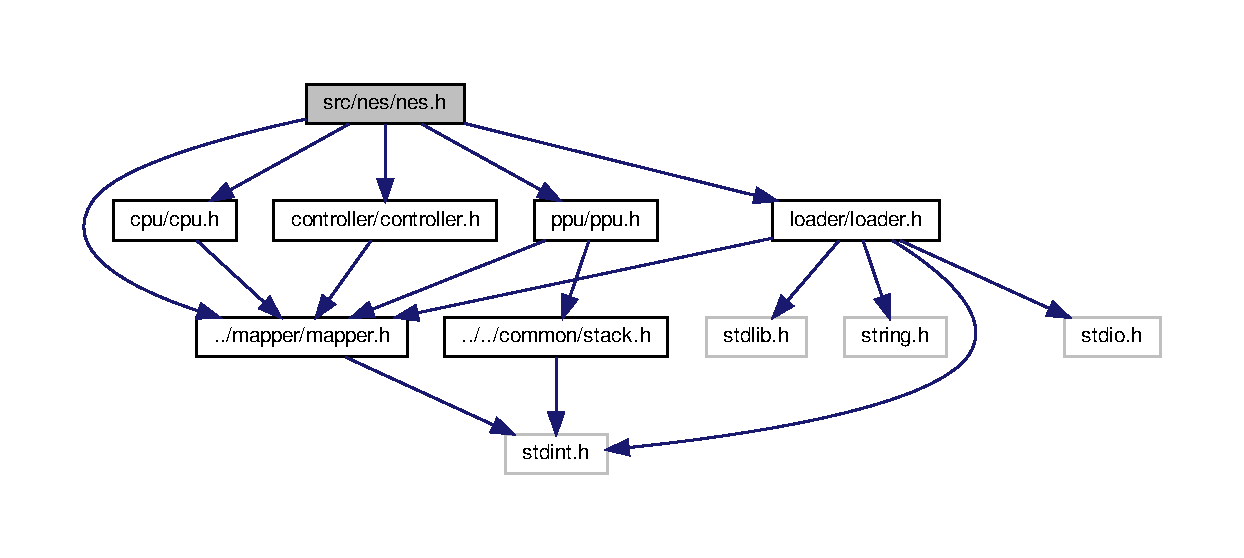
\includegraphics[width=350pt]{nes_8h__incl}
\end{center}
\end{figure}
This graph shows which files directly or indirectly include this file\+:\nopagebreak
\begin{figure}[H]
\begin{center}
\leavevmode
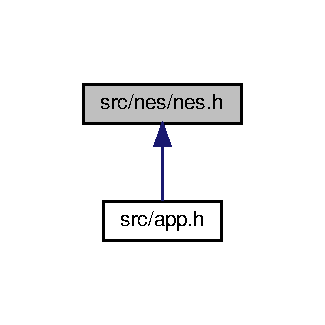
\includegraphics[width=156pt]{nes_8h__dep__incl}
\end{center}
\end{figure}
\subsection*{Data Structures}
\begin{DoxyCompactItemize}
\item 
struct \hyperlink{struct_n_e_s}{N\+ES}
\begin{DoxyCompactList}\small\item\em Hold every component to emulate the Nintendo Entertainement System. \end{DoxyCompactList}\end{DoxyCompactItemize}
\subsection*{Functions}
\begin{DoxyCompactItemize}
\item 
\hyperlink{struct_n_e_s}{N\+ES} $\ast$ \hyperlink{nes_8h_accb9617b500ae359028c76c4b5ebd9a4}{N\+E\+S\+\_\+\+Create} (char $\ast$filename)
\begin{DoxyCompactList}\small\item\em Allocate memory for the emulator and load the R\+OM provide in arg. \end{DoxyCompactList}\item 
uint8\+\_\+t \hyperlink{nes_8h_aed1b099550c90a2d72ee4d8b70b29c44}{N\+E\+S\+\_\+\+Next\+Frame} (\hyperlink{struct_n_e_s}{N\+ES} $\ast$self, uint16\+\_\+t keys\+Pressed)
\begin{DoxyCompactList}\small\item\em Execute the system for one frame. \end{DoxyCompactList}\item 
uint32\+\_\+t $\ast$ \hyperlink{nes_8h_aeaf5921177dae590ae91f5c4120edd83}{N\+E\+S\+\_\+\+Render} (\hyperlink{struct_n_e_s}{N\+ES} $\ast$self)
\begin{DoxyCompactList}\small\item\em Render image from \hyperlink{struct_p_p_u}{P\+PU}. \end{DoxyCompactList}\item 
void \hyperlink{nes_8h_a786a4a2ed4826ae60ff1f18c2120dc93}{N\+E\+S\+\_\+\+Destroy} (\hyperlink{struct_n_e_s}{N\+ES} $\ast$self)
\begin{DoxyCompactList}\small\item\em Free the memory used by the emulator. \end{DoxyCompactList}\end{DoxyCompactItemize}


\subsection{Detailed Description}
header file of \hyperlink{struct_n_e_s}{N\+ES} module 

\begin{DoxyAuthor}{Author}
Dylan Gageot 
\end{DoxyAuthor}
\begin{DoxyVersion}{Version}
1.\+0 
\end{DoxyVersion}
\begin{DoxyDate}{Date}
2019-\/02-\/25 
\end{DoxyDate}


\subsection{Function Documentation}
\mbox{\Hypertarget{nes_8h_accb9617b500ae359028c76c4b5ebd9a4}\label{nes_8h_accb9617b500ae359028c76c4b5ebd9a4}} 
\index{nes.\+h@{nes.\+h}!N\+E\+S\+\_\+\+Create@{N\+E\+S\+\_\+\+Create}}
\index{N\+E\+S\+\_\+\+Create@{N\+E\+S\+\_\+\+Create}!nes.\+h@{nes.\+h}}
\subsubsection{\texorpdfstring{N\+E\+S\+\_\+\+Create()}{NES\_Create()}}
{\footnotesize\ttfamily \hyperlink{struct_n_e_s}{N\+ES}$\ast$ N\+E\+S\+\_\+\+Create (\begin{DoxyParamCaption}\item[{char $\ast$}]{filename }\end{DoxyParamCaption})}



Allocate memory for the emulator and load the R\+OM provide in arg. 


\begin{DoxyParams}{Parameters}
{\em filename} & path that point a .nes file\\
\hline
\end{DoxyParams}
\begin{DoxyReturn}{Returns}
instance of \hyperlink{struct_n_e_s}{N\+ES} allocated 
\end{DoxyReturn}
\mbox{\Hypertarget{nes_8h_a786a4a2ed4826ae60ff1f18c2120dc93}\label{nes_8h_a786a4a2ed4826ae60ff1f18c2120dc93}} 
\index{nes.\+h@{nes.\+h}!N\+E\+S\+\_\+\+Destroy@{N\+E\+S\+\_\+\+Destroy}}
\index{N\+E\+S\+\_\+\+Destroy@{N\+E\+S\+\_\+\+Destroy}!nes.\+h@{nes.\+h}}
\subsubsection{\texorpdfstring{N\+E\+S\+\_\+\+Destroy()}{NES\_Destroy()}}
{\footnotesize\ttfamily void N\+E\+S\+\_\+\+Destroy (\begin{DoxyParamCaption}\item[{\hyperlink{struct_n_e_s}{N\+ES} $\ast$}]{self }\end{DoxyParamCaption})}



Free the memory used by the emulator. 


\begin{DoxyParams}{Parameters}
{\em self} & instance of \hyperlink{struct_n_e_s}{N\+ES} \\
\hline
\end{DoxyParams}
\mbox{\Hypertarget{nes_8h_aed1b099550c90a2d72ee4d8b70b29c44}\label{nes_8h_aed1b099550c90a2d72ee4d8b70b29c44}} 
\index{nes.\+h@{nes.\+h}!N\+E\+S\+\_\+\+Next\+Frame@{N\+E\+S\+\_\+\+Next\+Frame}}
\index{N\+E\+S\+\_\+\+Next\+Frame@{N\+E\+S\+\_\+\+Next\+Frame}!nes.\+h@{nes.\+h}}
\subsubsection{\texorpdfstring{N\+E\+S\+\_\+\+Next\+Frame()}{NES\_NextFrame()}}
{\footnotesize\ttfamily uint8\+\_\+t N\+E\+S\+\_\+\+Next\+Frame (\begin{DoxyParamCaption}\item[{\hyperlink{struct_n_e_s}{N\+ES} $\ast$}]{self,  }\item[{uint16\+\_\+t}]{keys\+Pressed }\end{DoxyParamCaption})}



Execute the system for one frame. 


\begin{DoxyParams}{Parameters}
{\em self} & instance of \hyperlink{struct_n_e_s}{N\+ES} \\
\hline
{\em keys\+Pressed} & keys pressed on keyboard \\
\hline
\end{DoxyParams}
\begin{DoxyReturn}{Returns}
E\+X\+I\+T\+\_\+\+S\+U\+C\+C\+E\+SS 
\end{DoxyReturn}
\mbox{\Hypertarget{nes_8h_aeaf5921177dae590ae91f5c4120edd83}\label{nes_8h_aeaf5921177dae590ae91f5c4120edd83}} 
\index{nes.\+h@{nes.\+h}!N\+E\+S\+\_\+\+Render@{N\+E\+S\+\_\+\+Render}}
\index{N\+E\+S\+\_\+\+Render@{N\+E\+S\+\_\+\+Render}!nes.\+h@{nes.\+h}}
\subsubsection{\texorpdfstring{N\+E\+S\+\_\+\+Render()}{NES\_Render()}}
{\footnotesize\ttfamily uint32\+\_\+t$\ast$ N\+E\+S\+\_\+\+Render (\begin{DoxyParamCaption}\item[{\hyperlink{struct_n_e_s}{N\+ES} $\ast$}]{self }\end{DoxyParamCaption})}



Render image from \hyperlink{struct_p_p_u}{P\+PU}. 


\begin{DoxyParams}{Parameters}
{\em self} & instance of \hyperlink{struct_n_e_s}{N\+ES}\\
\hline
\end{DoxyParams}
\begin{DoxyReturn}{Returns}
image array with color in 32 bits 
\end{DoxyReturn}

\hypertarget{ppu_8h}{}\section{src/nes/ppu/ppu.h File Reference}
\label{ppu_8h}\index{src/nes/ppu/ppu.\+h@{src/nes/ppu/ppu.\+h}}


header file of \hyperlink{struct_p_p_u}{P\+PU} module  


{\ttfamily \#include \char`\"{}../mapper/mapper.\+h\char`\"{}}\newline
{\ttfamily \#include \char`\"{}../../common/stack.\+h\char`\"{}}\newline
Include dependency graph for ppu.\+h\+:\nopagebreak
\begin{figure}[H]
\begin{center}
\leavevmode
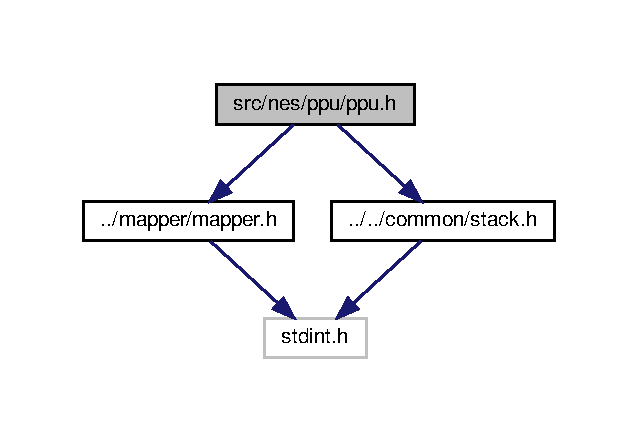
\includegraphics[width=306pt]{ppu_8h__incl}
\end{center}
\end{figure}
This graph shows which files directly or indirectly include this file\+:\nopagebreak
\begin{figure}[H]
\begin{center}
\leavevmode
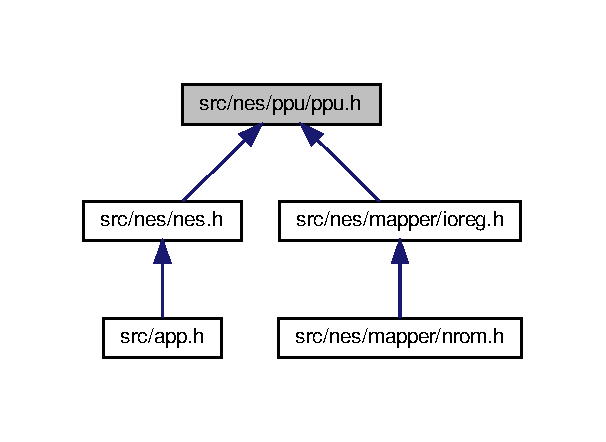
\includegraphics[width=291pt]{ppu_8h__dep__incl}
\end{center}
\end{figure}
\subsection*{Data Structures}
\begin{DoxyCompactItemize}
\item 
struct \hyperlink{struct_v_r_a_m}{V\+R\+AM}
\begin{DoxyCompactList}\small\item\em Hold pointer that is used to address \hyperlink{struct_v_r_a_m}{V\+R\+AM}. \end{DoxyCompactList}\item 
struct \hyperlink{struct_sprite}{Sprite}
\begin{DoxyCompactList}\small\item\em Hold registers for sprite rendering. \end{DoxyCompactList}\item 
struct \hyperlink{struct_p_p_u}{P\+PU}
\begin{DoxyCompactList}\small\item\em Hold every variable needed to run \hyperlink{struct_p_p_u}{P\+PU}. \end{DoxyCompactList}\end{DoxyCompactItemize}
\subsection*{Enumerations}
\begin{DoxyCompactItemize}
\item 
enum \hyperlink{ppu_8h_a25c6617f778fbdf0b8706596b50ea282}{State\+Sprite\+Evaluation} \{ \newline
\hyperlink{ppu_8h_a25c6617f778fbdf0b8706596b50ea282a0b9fe406d51e2fc0566a8efbdf0b5b3e}{S\+T\+A\+T\+E\+\_\+\+C\+O\+P\+Y\+\_\+Y} = 0, 
\hyperlink{ppu_8h_a25c6617f778fbdf0b8706596b50ea282a48f6cb0e9d0c137fa997dac3fce36626}{S\+T\+A\+T\+E\+\_\+\+C\+O\+P\+Y\+\_\+\+R\+E\+M\+A\+I\+N\+I\+NG}, 
\hyperlink{ppu_8h_a25c6617f778fbdf0b8706596b50ea282ac846900ca6ad1804a4b55e68cc60c88e}{S\+T\+A\+T\+E\+\_\+\+O\+V\+E\+R\+F\+L\+OW}, 
\hyperlink{ppu_8h_a25c6617f778fbdf0b8706596b50ea282a63ab7ce824fe58674bc0b3d6da10c8e1}{S\+T\+A\+T\+E\+\_\+\+O\+V\+E\+R\+F\+L\+O\+W\+\_\+\+R\+E\+M\+A\+I\+N\+I\+NG}, 
\newline
\hyperlink{ppu_8h_a25c6617f778fbdf0b8706596b50ea282a66d8f16a4988ddb948cc00bcdefafbb8}{S\+T\+A\+T\+E\+\_\+\+W\+A\+IT}
 \}\begin{DoxyCompactList}\small\item\em State for \hyperlink{struct_sprite}{Sprite} Evaluation algorithm. \end{DoxyCompactList}
\end{DoxyCompactItemize}
\subsection*{Functions}
\begin{DoxyCompactItemize}
\item 
char $\ast$ \hyperlink{ppu_8h_ae88906b300bd835c4b05be9305add112}{Render\+Color\+Palette} (void)
\begin{DoxyCompactList}\small\item\em Render 64 pixel with color palette of \hyperlink{struct_n_e_s}{N\+ES}. \end{DoxyCompactList}\item 
\hyperlink{struct_p_p_u}{P\+PU} $\ast$ \hyperlink{ppu_8h_a2705ad08aab791c5c8aa9499d888be0f}{P\+P\+U\+\_\+\+Create} (\hyperlink{struct_mapper}{Mapper} $\ast$mapper)
\begin{DoxyCompactList}\small\item\em Create instance of \hyperlink{struct_p_p_u}{P\+PU}. \end{DoxyCompactList}\item 
uint8\+\_\+t \hyperlink{ppu_8h_abd3b96cd2fb12c62b533b35e2771ef44}{P\+P\+U\+\_\+\+Init} (\hyperlink{struct_p_p_u}{P\+PU} $\ast$self)
\begin{DoxyCompactList}\small\item\em Initialize \hyperlink{struct_p_p_u}{P\+PU} structure. \end{DoxyCompactList}\item 
uint8\+\_\+t \hyperlink{ppu_8h_aa4ca6a4bf54eb93b1b63022babd347c1}{P\+P\+U\+\_\+\+Execute} (\hyperlink{struct_p_p_u}{P\+PU} $\ast$self, uint8\+\_\+t $\ast$context, uint8\+\_\+t clock)
\begin{DoxyCompactList}\small\item\em Execute \hyperlink{struct_p_p_u}{P\+PU} from a given timestamp. \end{DoxyCompactList}\item 
void \hyperlink{ppu_8h_af71022a2baf5cd766ea53117461825f6}{P\+P\+U\+\_\+\+Render\+Nametable} (\hyperlink{struct_p_p_u}{P\+PU} $\ast$self, uint32\+\_\+t $\ast$image, uint8\+\_\+t index)
\begin{DoxyCompactList}\small\item\em Draw a specified nametable into an array. \end{DoxyCompactList}\item 
void \hyperlink{ppu_8h_ae27ab418c06beecabbf275a8a1b5b0f5}{P\+P\+U\+\_\+\+Render\+Sprites} (\hyperlink{struct_p_p_u}{P\+PU} $\ast$self, uint32\+\_\+t $\ast$image)
\begin{DoxyCompactList}\small\item\em Draw sprite into an array. \end{DoxyCompactList}\item 
uint8\+\_\+t \hyperlink{ppu_8h_a82f4f31eab4a14a70047044299177a05}{P\+P\+U\+\_\+\+Picture\+Drawn} (\hyperlink{struct_p_p_u}{P\+PU} $\ast$self)
\begin{DoxyCompactList}\small\item\em Does the picture has been drawn by the component ? \end{DoxyCompactList}\item 
uint8\+\_\+t \hyperlink{ppu_8h_af5a63b31658c9a0e605cc11b075f0491}{P\+P\+U\+\_\+\+Update\+Cycle} (\hyperlink{struct_p_p_u}{P\+PU} $\ast$self)
\begin{DoxyCompactList}\small\item\em Increment cycle and scanline. \end{DoxyCompactList}\item 
uint8\+\_\+t \hyperlink{ppu_8h_a72790c3314d70ef3e84b1842a6b20952}{P\+P\+U\+\_\+\+Check\+Register} (\hyperlink{struct_p_p_u}{P\+PU} $\ast$self)
\begin{DoxyCompactList}\small\item\em Update registers in case of access from \hyperlink{struct_c_p_u}{C\+PU}. \end{DoxyCompactList}\item 
uint8\+\_\+t \hyperlink{ppu_8h_a8e4e1b256bb3e995ee71ef1cb32d70a5}{P\+P\+U\+\_\+\+Manage\+Timing} (\hyperlink{struct_p_p_u}{P\+PU} $\ast$self, \hyperlink{struct_stack}{Stack} $\ast$task\+List)
\begin{DoxyCompactList}\small\item\em Fill a stack F\+I\+LO with tasks to execute at a specific cycle. \end{DoxyCompactList}\item 
uint8\+\_\+t \hyperlink{ppu_8h_a41f63ff9039e460ffe082d7ffe0d90c7}{P\+P\+U\+\_\+\+Clear\+Flag} (\hyperlink{struct_p_p_u}{P\+PU} $\ast$self)
\begin{DoxyCompactList}\small\item\em Clear Vertical Blank and \hyperlink{struct_sprite}{Sprite} 0 flag. \end{DoxyCompactList}\item 
uint8\+\_\+t \hyperlink{ppu_8h_a8faf6d01ea33cef8a408b5eac805d1a5}{P\+P\+U\+\_\+\+Set\+Flag} (\hyperlink{struct_p_p_u}{P\+PU} $\ast$self)
\begin{DoxyCompactList}\small\item\em Set Vertical Blank flag. \end{DoxyCompactList}\item 
uint8\+\_\+t \hyperlink{ppu_8h_aed74b3709cc1ee1f05a7a443fb471c89}{P\+P\+U\+\_\+\+Increment\+CorseX} (\hyperlink{struct_p_p_u}{P\+PU} $\ast$self)
\begin{DoxyCompactList}\small\item\em Increment Corse X component in \hyperlink{struct_v_r_a_m_ac5f38113a34f9eab3e7782eade81d266}{V\+R\+A\+M.\+v}. \end{DoxyCompactList}\item 
uint8\+\_\+t \hyperlink{ppu_8h_a44eb857409f79ed652debf0a2c0f80aa}{P\+P\+U\+\_\+\+IncrementY} (\hyperlink{struct_p_p_u}{P\+PU} $\ast$self)
\begin{DoxyCompactList}\small\item\em Increment Y component in \hyperlink{struct_v_r_a_m_ac5f38113a34f9eab3e7782eade81d266}{V\+R\+A\+M.\+v}. \end{DoxyCompactList}\item 
uint8\+\_\+t \hyperlink{ppu_8h_a4ce17e4f85d86dc05e919ba40bbd8f77}{P\+P\+U\+\_\+\+ManageV} (\hyperlink{struct_p_p_u}{P\+PU} $\ast$self)
\begin{DoxyCompactList}\small\item\em Manage increment and boundaries of \hyperlink{struct_v_r_a_m_ac5f38113a34f9eab3e7782eade81d266}{V\+R\+A\+M.\+v}. \end{DoxyCompactList}\item 
uint8\+\_\+t \hyperlink{ppu_8h_a884996fed5df03af906f961fb586955e}{P\+P\+U\+\_\+\+Clear\+Secondary\+O\+AM} (\hyperlink{struct_p_p_u}{P\+PU} $\ast$self)
\begin{DoxyCompactList}\small\item\em Clear Secondary O\+AM. \end{DoxyCompactList}\item 
uint8\+\_\+t \hyperlink{ppu_8h_ad2f329d145cc7dc3e13ea4fc8a8d5851}{P\+P\+U\+\_\+\+Refresh\+Register} (\hyperlink{struct_p_p_u}{P\+PU} $\ast$self, uint8\+\_\+t $\ast$context)
\begin{DoxyCompactList}\small\item\em Refresh registers after \hyperlink{struct_p_p_u}{P\+PU} execution. \end{DoxyCompactList}\item 
uint8\+\_\+t \hyperlink{ppu_8h_a1d5e092e141bf29995ca6531f606ae88}{P\+P\+U\+\_\+\+Fetch\+Tile} (\hyperlink{struct_p_p_u}{P\+PU} $\ast$self)
\begin{DoxyCompactList}\small\item\em Fill internal shift registers for background rendering. \end{DoxyCompactList}\item 
uint8\+\_\+t \hyperlink{ppu_8h_a923a8dfa05010097cf173cfc278360f0}{P\+P\+U\+\_\+\+Sprite\+Evaluation} (\hyperlink{struct_p_p_u}{P\+PU} $\ast$self)
\begin{DoxyCompactList}\small\item\em Fill secondary O\+AM with sprite to be rendered on the next scanline. \end{DoxyCompactList}\item 
uint8\+\_\+t \hyperlink{ppu_8h_a6757844f4db33d1c9a202280a0cb84c4}{P\+P\+U\+\_\+\+Fetch\+Sprite} (\hyperlink{struct_p_p_u}{P\+PU} $\ast$self)
\begin{DoxyCompactList}\small\item\em Fill internal shift registers for sprites rendering of next scanline. \end{DoxyCompactList}\item 
uint8\+\_\+t \hyperlink{ppu_8h_a4ade9d0f5bcbf6ce44d062fb07d77479}{P\+P\+U\+\_\+\+Draw} (\hyperlink{struct_p_p_u}{P\+PU} $\ast$self)
\begin{DoxyCompactList}\small\item\em Draw at a specific pixel directed by scanline and cycle counter. \end{DoxyCompactList}\item 
void \hyperlink{ppu_8h_a47d0d84eb1aa8893d37dfad9e4442177}{P\+P\+U\+\_\+\+Destroy} (\hyperlink{struct_p_p_u}{P\+PU} $\ast$self)
\begin{DoxyCompactList}\small\item\em Destroy instance of \hyperlink{struct_p_p_u}{P\+PU}. \end{DoxyCompactList}\end{DoxyCompactItemize}


\subsection{Detailed Description}
header file of \hyperlink{struct_p_p_u}{P\+PU} module 

\begin{DoxyAuthor}{Author}
Dylan Gageot 
\end{DoxyAuthor}
\begin{DoxyVersion}{Version}
1.\+0 
\end{DoxyVersion}
\begin{DoxyDate}{Date}
2019-\/03-\/31 
\end{DoxyDate}


\subsection{Enumeration Type Documentation}
\mbox{\Hypertarget{ppu_8h_a25c6617f778fbdf0b8706596b50ea282}\label{ppu_8h_a25c6617f778fbdf0b8706596b50ea282}} 
\index{ppu.\+h@{ppu.\+h}!State\+Sprite\+Evaluation@{State\+Sprite\+Evaluation}}
\index{State\+Sprite\+Evaluation@{State\+Sprite\+Evaluation}!ppu.\+h@{ppu.\+h}}
\subsubsection{\texorpdfstring{State\+Sprite\+Evaluation}{StateSpriteEvaluation}}
{\footnotesize\ttfamily enum \hyperlink{ppu_8h_a25c6617f778fbdf0b8706596b50ea282}{State\+Sprite\+Evaluation}}



State for \hyperlink{struct_sprite}{Sprite} Evaluation algorithm. 

\begin{DoxyEnumFields}{Enumerator}
\raisebox{\heightof{T}}[0pt][0pt]{\index{S\+T\+A\+T\+E\+\_\+\+C\+O\+P\+Y\+\_\+Y@{S\+T\+A\+T\+E\+\_\+\+C\+O\+P\+Y\+\_\+Y}!ppu.\+h@{ppu.\+h}}\index{ppu.\+h@{ppu.\+h}!S\+T\+A\+T\+E\+\_\+\+C\+O\+P\+Y\+\_\+Y@{S\+T\+A\+T\+E\+\_\+\+C\+O\+P\+Y\+\_\+Y}}}\mbox{\Hypertarget{ppu_8h_a25c6617f778fbdf0b8706596b50ea282a0b9fe406d51e2fc0566a8efbdf0b5b3e}\label{ppu_8h_a25c6617f778fbdf0b8706596b50ea282a0b9fe406d51e2fc0566a8efbdf0b5b3e}} 
S\+T\+A\+T\+E\+\_\+\+C\+O\+P\+Y\+\_\+Y&Y-\/coordonate copy from O\+AM to S\+O\+AM \\
\hline

\raisebox{\heightof{T}}[0pt][0pt]{\index{S\+T\+A\+T\+E\+\_\+\+C\+O\+P\+Y\+\_\+\+R\+E\+M\+A\+I\+N\+I\+NG@{S\+T\+A\+T\+E\+\_\+\+C\+O\+P\+Y\+\_\+\+R\+E\+M\+A\+I\+N\+I\+NG}!ppu.\+h@{ppu.\+h}}\index{ppu.\+h@{ppu.\+h}!S\+T\+A\+T\+E\+\_\+\+C\+O\+P\+Y\+\_\+\+R\+E\+M\+A\+I\+N\+I\+NG@{S\+T\+A\+T\+E\+\_\+\+C\+O\+P\+Y\+\_\+\+R\+E\+M\+A\+I\+N\+I\+NG}}}\mbox{\Hypertarget{ppu_8h_a25c6617f778fbdf0b8706596b50ea282a48f6cb0e9d0c137fa997dac3fce36626}\label{ppu_8h_a25c6617f778fbdf0b8706596b50ea282a48f6cb0e9d0c137fa997dac3fce36626}} 
S\+T\+A\+T\+E\+\_\+\+C\+O\+P\+Y\+\_\+\+R\+E\+M\+A\+I\+N\+I\+NG&Copy remaining 3 byte from O\+AM to S\+O\+AM \\
\hline

\raisebox{\heightof{T}}[0pt][0pt]{\index{S\+T\+A\+T\+E\+\_\+\+O\+V\+E\+R\+F\+L\+OW@{S\+T\+A\+T\+E\+\_\+\+O\+V\+E\+R\+F\+L\+OW}!ppu.\+h@{ppu.\+h}}\index{ppu.\+h@{ppu.\+h}!S\+T\+A\+T\+E\+\_\+\+O\+V\+E\+R\+F\+L\+OW@{S\+T\+A\+T\+E\+\_\+\+O\+V\+E\+R\+F\+L\+OW}}}\mbox{\Hypertarget{ppu_8h_a25c6617f778fbdf0b8706596b50ea282ac846900ca6ad1804a4b55e68cc60c88e}\label{ppu_8h_a25c6617f778fbdf0b8706596b50ea282ac846900ca6ad1804a4b55e68cc60c88e}} 
S\+T\+A\+T\+E\+\_\+\+O\+V\+E\+R\+F\+L\+OW&8 sprites has been written in S\+O\+AM \\
\hline

\raisebox{\heightof{T}}[0pt][0pt]{\index{S\+T\+A\+T\+E\+\_\+\+O\+V\+E\+R\+F\+L\+O\+W\+\_\+\+R\+E\+M\+A\+I\+N\+I\+NG@{S\+T\+A\+T\+E\+\_\+\+O\+V\+E\+R\+F\+L\+O\+W\+\_\+\+R\+E\+M\+A\+I\+N\+I\+NG}!ppu.\+h@{ppu.\+h}}\index{ppu.\+h@{ppu.\+h}!S\+T\+A\+T\+E\+\_\+\+O\+V\+E\+R\+F\+L\+O\+W\+\_\+\+R\+E\+M\+A\+I\+N\+I\+NG@{S\+T\+A\+T\+E\+\_\+\+O\+V\+E\+R\+F\+L\+O\+W\+\_\+\+R\+E\+M\+A\+I\+N\+I\+NG}}}\mbox{\Hypertarget{ppu_8h_a25c6617f778fbdf0b8706596b50ea282a63ab7ce824fe58674bc0b3d6da10c8e1}\label{ppu_8h_a25c6617f778fbdf0b8706596b50ea282a63ab7ce824fe58674bc0b3d6da10c8e1}} 
S\+T\+A\+T\+E\+\_\+\+O\+V\+E\+R\+F\+L\+O\+W\+\_\+\+R\+E\+M\+A\+I\+N\+I\+NG&\hyperlink{struct_sprite}{Sprite} overflow has occured \\
\hline

\raisebox{\heightof{T}}[0pt][0pt]{\index{S\+T\+A\+T\+E\+\_\+\+W\+A\+IT@{S\+T\+A\+T\+E\+\_\+\+W\+A\+IT}!ppu.\+h@{ppu.\+h}}\index{ppu.\+h@{ppu.\+h}!S\+T\+A\+T\+E\+\_\+\+W\+A\+IT@{S\+T\+A\+T\+E\+\_\+\+W\+A\+IT}}}\mbox{\Hypertarget{ppu_8h_a25c6617f778fbdf0b8706596b50ea282a66d8f16a4988ddb948cc00bcdefafbb8}\label{ppu_8h_a25c6617f778fbdf0b8706596b50ea282a66d8f16a4988ddb948cc00bcdefafbb8}} 
S\+T\+A\+T\+E\+\_\+\+W\+A\+IT&All sprites has been evaluated \\
\hline

\end{DoxyEnumFields}


\subsection{Function Documentation}
\mbox{\Hypertarget{ppu_8h_a72790c3314d70ef3e84b1842a6b20952}\label{ppu_8h_a72790c3314d70ef3e84b1842a6b20952}} 
\index{ppu.\+h@{ppu.\+h}!P\+P\+U\+\_\+\+Check\+Register@{P\+P\+U\+\_\+\+Check\+Register}}
\index{P\+P\+U\+\_\+\+Check\+Register@{P\+P\+U\+\_\+\+Check\+Register}!ppu.\+h@{ppu.\+h}}
\subsubsection{\texorpdfstring{P\+P\+U\+\_\+\+Check\+Register()}{PPU\_CheckRegister()}}
{\footnotesize\ttfamily uint8\+\_\+t P\+P\+U\+\_\+\+Check\+Register (\begin{DoxyParamCaption}\item[{\hyperlink{struct_p_p_u}{P\+PU} $\ast$}]{self }\end{DoxyParamCaption})}



Update registers in case of access from \hyperlink{struct_c_p_u}{C\+PU}. 


\begin{DoxyParams}{Parameters}
{\em self} & instance of \hyperlink{struct_p_p_u}{P\+PU}\\
\hline
\end{DoxyParams}
\begin{DoxyReturn}{Returns}
E\+X\+I\+T\+\_\+\+S\+U\+C\+C\+E\+SS if succeed, E\+X\+I\+T\+\_\+\+F\+A\+I\+L\+U\+RE otherwise 
\end{DoxyReturn}
\mbox{\Hypertarget{ppu_8h_a41f63ff9039e460ffe082d7ffe0d90c7}\label{ppu_8h_a41f63ff9039e460ffe082d7ffe0d90c7}} 
\index{ppu.\+h@{ppu.\+h}!P\+P\+U\+\_\+\+Clear\+Flag@{P\+P\+U\+\_\+\+Clear\+Flag}}
\index{P\+P\+U\+\_\+\+Clear\+Flag@{P\+P\+U\+\_\+\+Clear\+Flag}!ppu.\+h@{ppu.\+h}}
\subsubsection{\texorpdfstring{P\+P\+U\+\_\+\+Clear\+Flag()}{PPU\_ClearFlag()}}
{\footnotesize\ttfamily uint8\+\_\+t P\+P\+U\+\_\+\+Clear\+Flag (\begin{DoxyParamCaption}\item[{\hyperlink{struct_p_p_u}{P\+PU} $\ast$}]{self }\end{DoxyParamCaption})}



Clear Vertical Blank and \hyperlink{struct_sprite}{Sprite} 0 flag. 


\begin{DoxyParams}{Parameters}
{\em self} & instance of \hyperlink{struct_p_p_u}{P\+PU}\\
\hline
\end{DoxyParams}
\begin{DoxyReturn}{Returns}
E\+X\+I\+T\+\_\+\+S\+U\+C\+C\+E\+SS if succeed, E\+X\+I\+T\+\_\+\+F\+A\+I\+L\+U\+RE otherwise 
\end{DoxyReturn}
\mbox{\Hypertarget{ppu_8h_a884996fed5df03af906f961fb586955e}\label{ppu_8h_a884996fed5df03af906f961fb586955e}} 
\index{ppu.\+h@{ppu.\+h}!P\+P\+U\+\_\+\+Clear\+Secondary\+O\+AM@{P\+P\+U\+\_\+\+Clear\+Secondary\+O\+AM}}
\index{P\+P\+U\+\_\+\+Clear\+Secondary\+O\+AM@{P\+P\+U\+\_\+\+Clear\+Secondary\+O\+AM}!ppu.\+h@{ppu.\+h}}
\subsubsection{\texorpdfstring{P\+P\+U\+\_\+\+Clear\+Secondary\+O\+A\+M()}{PPU\_ClearSecondaryOAM()}}
{\footnotesize\ttfamily uint8\+\_\+t P\+P\+U\+\_\+\+Clear\+Secondary\+O\+AM (\begin{DoxyParamCaption}\item[{\hyperlink{struct_p_p_u}{P\+PU} $\ast$}]{self }\end{DoxyParamCaption})}



Clear Secondary O\+AM. 


\begin{DoxyParams}{Parameters}
{\em self} & instance of \hyperlink{struct_p_p_u}{P\+PU}\\
\hline
\end{DoxyParams}
\begin{DoxyReturn}{Returns}
E\+X\+I\+T\+\_\+\+S\+U\+C\+C\+E\+SS if succeed, E\+X\+I\+T\+\_\+\+F\+A\+I\+L\+U\+RE otherwise 
\end{DoxyReturn}
\mbox{\Hypertarget{ppu_8h_a2705ad08aab791c5c8aa9499d888be0f}\label{ppu_8h_a2705ad08aab791c5c8aa9499d888be0f}} 
\index{ppu.\+h@{ppu.\+h}!P\+P\+U\+\_\+\+Create@{P\+P\+U\+\_\+\+Create}}
\index{P\+P\+U\+\_\+\+Create@{P\+P\+U\+\_\+\+Create}!ppu.\+h@{ppu.\+h}}
\subsubsection{\texorpdfstring{P\+P\+U\+\_\+\+Create()}{PPU\_Create()}}
{\footnotesize\ttfamily \hyperlink{struct_p_p_u}{P\+PU}$\ast$ P\+P\+U\+\_\+\+Create (\begin{DoxyParamCaption}\item[{\hyperlink{struct_mapper}{Mapper} $\ast$}]{mapper }\end{DoxyParamCaption})}



Create instance of \hyperlink{struct_p_p_u}{P\+PU}. 


\begin{DoxyParams}{Parameters}
{\em mapper} & instance of \hyperlink{struct_mapper}{Mapper}\\
\hline
\end{DoxyParams}
\begin{DoxyReturn}{Returns}
instance of \hyperlink{struct_p_p_u}{P\+PU} 
\end{DoxyReturn}
\mbox{\Hypertarget{ppu_8h_a47d0d84eb1aa8893d37dfad9e4442177}\label{ppu_8h_a47d0d84eb1aa8893d37dfad9e4442177}} 
\index{ppu.\+h@{ppu.\+h}!P\+P\+U\+\_\+\+Destroy@{P\+P\+U\+\_\+\+Destroy}}
\index{P\+P\+U\+\_\+\+Destroy@{P\+P\+U\+\_\+\+Destroy}!ppu.\+h@{ppu.\+h}}
\subsubsection{\texorpdfstring{P\+P\+U\+\_\+\+Destroy()}{PPU\_Destroy()}}
{\footnotesize\ttfamily void P\+P\+U\+\_\+\+Destroy (\begin{DoxyParamCaption}\item[{\hyperlink{struct_p_p_u}{P\+PU} $\ast$}]{self }\end{DoxyParamCaption})}



Destroy instance of \hyperlink{struct_p_p_u}{P\+PU}. 


\begin{DoxyParams}{Parameters}
{\em self} & instance of \hyperlink{struct_p_p_u}{P\+PU} \\
\hline
\end{DoxyParams}
\mbox{\Hypertarget{ppu_8h_a4ade9d0f5bcbf6ce44d062fb07d77479}\label{ppu_8h_a4ade9d0f5bcbf6ce44d062fb07d77479}} 
\index{ppu.\+h@{ppu.\+h}!P\+P\+U\+\_\+\+Draw@{P\+P\+U\+\_\+\+Draw}}
\index{P\+P\+U\+\_\+\+Draw@{P\+P\+U\+\_\+\+Draw}!ppu.\+h@{ppu.\+h}}
\subsubsection{\texorpdfstring{P\+P\+U\+\_\+\+Draw()}{PPU\_Draw()}}
{\footnotesize\ttfamily uint8\+\_\+t P\+P\+U\+\_\+\+Draw (\begin{DoxyParamCaption}\item[{\hyperlink{struct_p_p_u}{P\+PU} $\ast$}]{self }\end{DoxyParamCaption})}



Draw at a specific pixel directed by scanline and cycle counter. 


\begin{DoxyParams}{Parameters}
{\em self} & instance of \hyperlink{struct_p_p_u}{P\+PU}\\
\hline
\end{DoxyParams}
\begin{DoxyReturn}{Returns}
E\+X\+I\+T\+\_\+\+S\+U\+C\+C\+E\+SS if succeed, E\+X\+I\+T\+\_\+\+F\+A\+I\+L\+U\+RE otherwise 
\end{DoxyReturn}
\mbox{\Hypertarget{ppu_8h_aa4ca6a4bf54eb93b1b63022babd347c1}\label{ppu_8h_aa4ca6a4bf54eb93b1b63022babd347c1}} 
\index{ppu.\+h@{ppu.\+h}!P\+P\+U\+\_\+\+Execute@{P\+P\+U\+\_\+\+Execute}}
\index{P\+P\+U\+\_\+\+Execute@{P\+P\+U\+\_\+\+Execute}!ppu.\+h@{ppu.\+h}}
\subsubsection{\texorpdfstring{P\+P\+U\+\_\+\+Execute()}{PPU\_Execute()}}
{\footnotesize\ttfamily uint8\+\_\+t P\+P\+U\+\_\+\+Execute (\begin{DoxyParamCaption}\item[{\hyperlink{struct_p_p_u}{P\+PU} $\ast$}]{self,  }\item[{uint8\+\_\+t $\ast$}]{context,  }\item[{uint8\+\_\+t}]{clock }\end{DoxyParamCaption})}



Execute \hyperlink{struct_p_p_u}{P\+PU} from a given timestamp. 


\begin{DoxyParams}{Parameters}
{\em self} & instance of \hyperlink{struct_p_p_u}{P\+PU} \\
\hline
{\em context} & wire through every component \\
\hline
{\em clock} & number of \hyperlink{struct_p_p_u}{P\+PU} cycle to consumme\\
\hline
\end{DoxyParams}
\begin{DoxyReturn}{Returns}
E\+X\+I\+T\+\_\+\+S\+U\+C\+C\+E\+SS if succeed, E\+X\+I\+T\+\_\+\+F\+A\+I\+L\+U\+RE otherwise 
\end{DoxyReturn}
\mbox{\Hypertarget{ppu_8h_a6757844f4db33d1c9a202280a0cb84c4}\label{ppu_8h_a6757844f4db33d1c9a202280a0cb84c4}} 
\index{ppu.\+h@{ppu.\+h}!P\+P\+U\+\_\+\+Fetch\+Sprite@{P\+P\+U\+\_\+\+Fetch\+Sprite}}
\index{P\+P\+U\+\_\+\+Fetch\+Sprite@{P\+P\+U\+\_\+\+Fetch\+Sprite}!ppu.\+h@{ppu.\+h}}
\subsubsection{\texorpdfstring{P\+P\+U\+\_\+\+Fetch\+Sprite()}{PPU\_FetchSprite()}}
{\footnotesize\ttfamily uint8\+\_\+t P\+P\+U\+\_\+\+Fetch\+Sprite (\begin{DoxyParamCaption}\item[{\hyperlink{struct_p_p_u}{P\+PU} $\ast$}]{self }\end{DoxyParamCaption})}



Fill internal shift registers for sprites rendering of next scanline. 


\begin{DoxyParams}{Parameters}
{\em self} & instance of \hyperlink{struct_p_p_u}{P\+PU}\\
\hline
\end{DoxyParams}
\begin{DoxyReturn}{Returns}
E\+X\+I\+T\+\_\+\+S\+U\+C\+C\+E\+SS if succeed, E\+X\+I\+T\+\_\+\+F\+A\+I\+L\+U\+RE otherwise 
\end{DoxyReturn}
\mbox{\Hypertarget{ppu_8h_a1d5e092e141bf29995ca6531f606ae88}\label{ppu_8h_a1d5e092e141bf29995ca6531f606ae88}} 
\index{ppu.\+h@{ppu.\+h}!P\+P\+U\+\_\+\+Fetch\+Tile@{P\+P\+U\+\_\+\+Fetch\+Tile}}
\index{P\+P\+U\+\_\+\+Fetch\+Tile@{P\+P\+U\+\_\+\+Fetch\+Tile}!ppu.\+h@{ppu.\+h}}
\subsubsection{\texorpdfstring{P\+P\+U\+\_\+\+Fetch\+Tile()}{PPU\_FetchTile()}}
{\footnotesize\ttfamily uint8\+\_\+t P\+P\+U\+\_\+\+Fetch\+Tile (\begin{DoxyParamCaption}\item[{\hyperlink{struct_p_p_u}{P\+PU} $\ast$}]{self }\end{DoxyParamCaption})}



Fill internal shift registers for background rendering. 


\begin{DoxyParams}{Parameters}
{\em self} & instance of \hyperlink{struct_p_p_u}{P\+PU}\\
\hline
\end{DoxyParams}
\begin{DoxyReturn}{Returns}
E\+X\+I\+T\+\_\+\+S\+U\+C\+C\+E\+SS if succeed, E\+X\+I\+T\+\_\+\+F\+A\+I\+L\+U\+RE otherwise 
\end{DoxyReturn}
\mbox{\Hypertarget{ppu_8h_aed74b3709cc1ee1f05a7a443fb471c89}\label{ppu_8h_aed74b3709cc1ee1f05a7a443fb471c89}} 
\index{ppu.\+h@{ppu.\+h}!P\+P\+U\+\_\+\+Increment\+CorseX@{P\+P\+U\+\_\+\+Increment\+CorseX}}
\index{P\+P\+U\+\_\+\+Increment\+CorseX@{P\+P\+U\+\_\+\+Increment\+CorseX}!ppu.\+h@{ppu.\+h}}
\subsubsection{\texorpdfstring{P\+P\+U\+\_\+\+Increment\+Corse\+X()}{PPU\_IncrementCorseX()}}
{\footnotesize\ttfamily uint8\+\_\+t P\+P\+U\+\_\+\+Increment\+CorseX (\begin{DoxyParamCaption}\item[{\hyperlink{struct_p_p_u}{P\+PU} $\ast$}]{self }\end{DoxyParamCaption})}



Increment Corse X component in \hyperlink{struct_v_r_a_m_ac5f38113a34f9eab3e7782eade81d266}{V\+R\+A\+M.\+v}. 


\begin{DoxyParams}{Parameters}
{\em self} & instance of \hyperlink{struct_p_p_u}{P\+PU}\\
\hline
\end{DoxyParams}
\begin{DoxyReturn}{Returns}
E\+X\+I\+T\+\_\+\+S\+U\+C\+C\+E\+SS if succeed, E\+X\+I\+T\+\_\+\+F\+A\+I\+L\+U\+RE otherwise 
\end{DoxyReturn}
\mbox{\Hypertarget{ppu_8h_a44eb857409f79ed652debf0a2c0f80aa}\label{ppu_8h_a44eb857409f79ed652debf0a2c0f80aa}} 
\index{ppu.\+h@{ppu.\+h}!P\+P\+U\+\_\+\+IncrementY@{P\+P\+U\+\_\+\+IncrementY}}
\index{P\+P\+U\+\_\+\+IncrementY@{P\+P\+U\+\_\+\+IncrementY}!ppu.\+h@{ppu.\+h}}
\subsubsection{\texorpdfstring{P\+P\+U\+\_\+\+Increment\+Y()}{PPU\_IncrementY()}}
{\footnotesize\ttfamily uint8\+\_\+t P\+P\+U\+\_\+\+IncrementY (\begin{DoxyParamCaption}\item[{\hyperlink{struct_p_p_u}{P\+PU} $\ast$}]{self }\end{DoxyParamCaption})}



Increment Y component in \hyperlink{struct_v_r_a_m_ac5f38113a34f9eab3e7782eade81d266}{V\+R\+A\+M.\+v}. 


\begin{DoxyParams}{Parameters}
{\em self} & instance of \hyperlink{struct_p_p_u}{P\+PU}\\
\hline
\end{DoxyParams}
\begin{DoxyReturn}{Returns}
E\+X\+I\+T\+\_\+\+S\+U\+C\+C\+E\+SS if succeed, E\+X\+I\+T\+\_\+\+F\+A\+I\+L\+U\+RE otherwise 
\end{DoxyReturn}
\mbox{\Hypertarget{ppu_8h_abd3b96cd2fb12c62b533b35e2771ef44}\label{ppu_8h_abd3b96cd2fb12c62b533b35e2771ef44}} 
\index{ppu.\+h@{ppu.\+h}!P\+P\+U\+\_\+\+Init@{P\+P\+U\+\_\+\+Init}}
\index{P\+P\+U\+\_\+\+Init@{P\+P\+U\+\_\+\+Init}!ppu.\+h@{ppu.\+h}}
\subsubsection{\texorpdfstring{P\+P\+U\+\_\+\+Init()}{PPU\_Init()}}
{\footnotesize\ttfamily uint8\+\_\+t P\+P\+U\+\_\+\+Init (\begin{DoxyParamCaption}\item[{\hyperlink{struct_p_p_u}{P\+PU} $\ast$}]{self }\end{DoxyParamCaption})}



Initialize \hyperlink{struct_p_p_u}{P\+PU} structure. 


\begin{DoxyParams}{Parameters}
{\em self} & instance of \hyperlink{struct_p_p_u}{P\+PU}\\
\hline
\end{DoxyParams}
\begin{DoxyReturn}{Returns}
E\+X\+I\+T\+\_\+\+S\+U\+C\+C\+E\+SS if succeed, E\+X\+I\+T\+\_\+\+F\+A\+I\+L\+U\+RE otherwise 
\end{DoxyReturn}
\mbox{\Hypertarget{ppu_8h_a8e4e1b256bb3e995ee71ef1cb32d70a5}\label{ppu_8h_a8e4e1b256bb3e995ee71ef1cb32d70a5}} 
\index{ppu.\+h@{ppu.\+h}!P\+P\+U\+\_\+\+Manage\+Timing@{P\+P\+U\+\_\+\+Manage\+Timing}}
\index{P\+P\+U\+\_\+\+Manage\+Timing@{P\+P\+U\+\_\+\+Manage\+Timing}!ppu.\+h@{ppu.\+h}}
\subsubsection{\texorpdfstring{P\+P\+U\+\_\+\+Manage\+Timing()}{PPU\_ManageTiming()}}
{\footnotesize\ttfamily uint8\+\_\+t P\+P\+U\+\_\+\+Manage\+Timing (\begin{DoxyParamCaption}\item[{\hyperlink{struct_p_p_u}{P\+PU} $\ast$}]{self,  }\item[{\hyperlink{struct_stack}{Stack} $\ast$}]{task\+List }\end{DoxyParamCaption})}



Fill a stack F\+I\+LO with tasks to execute at a specific cycle. 


\begin{DoxyParams}{Parameters}
{\em self} & instance of \hyperlink{struct_p_p_u}{P\+PU} \\
\hline
{\em task\+List} & instance of \hyperlink{struct_stack}{Stack} to schedule task to execute\\
\hline
\end{DoxyParams}
\begin{DoxyReturn}{Returns}
E\+X\+I\+T\+\_\+\+S\+U\+C\+C\+E\+SS if succeed, E\+X\+I\+T\+\_\+\+F\+A\+I\+L\+U\+RE otherwise 
\end{DoxyReturn}
\mbox{\Hypertarget{ppu_8h_a4ce17e4f85d86dc05e919ba40bbd8f77}\label{ppu_8h_a4ce17e4f85d86dc05e919ba40bbd8f77}} 
\index{ppu.\+h@{ppu.\+h}!P\+P\+U\+\_\+\+ManageV@{P\+P\+U\+\_\+\+ManageV}}
\index{P\+P\+U\+\_\+\+ManageV@{P\+P\+U\+\_\+\+ManageV}!ppu.\+h@{ppu.\+h}}
\subsubsection{\texorpdfstring{P\+P\+U\+\_\+\+Manage\+V()}{PPU\_ManageV()}}
{\footnotesize\ttfamily uint8\+\_\+t P\+P\+U\+\_\+\+ManageV (\begin{DoxyParamCaption}\item[{\hyperlink{struct_p_p_u}{P\+PU} $\ast$}]{self }\end{DoxyParamCaption})}



Manage increment and boundaries of \hyperlink{struct_v_r_a_m_ac5f38113a34f9eab3e7782eade81d266}{V\+R\+A\+M.\+v}. 


\begin{DoxyParams}{Parameters}
{\em self} & instance of \hyperlink{struct_p_p_u}{P\+PU}\\
\hline
\end{DoxyParams}
\begin{DoxyReturn}{Returns}
E\+X\+I\+T\+\_\+\+S\+U\+C\+C\+E\+SS if succeed, E\+X\+I\+T\+\_\+\+F\+A\+I\+L\+U\+RE otherwise 
\end{DoxyReturn}
\mbox{\Hypertarget{ppu_8h_a82f4f31eab4a14a70047044299177a05}\label{ppu_8h_a82f4f31eab4a14a70047044299177a05}} 
\index{ppu.\+h@{ppu.\+h}!P\+P\+U\+\_\+\+Picture\+Drawn@{P\+P\+U\+\_\+\+Picture\+Drawn}}
\index{P\+P\+U\+\_\+\+Picture\+Drawn@{P\+P\+U\+\_\+\+Picture\+Drawn}!ppu.\+h@{ppu.\+h}}
\subsubsection{\texorpdfstring{P\+P\+U\+\_\+\+Picture\+Drawn()}{PPU\_PictureDrawn()}}
{\footnotesize\ttfamily uint8\+\_\+t P\+P\+U\+\_\+\+Picture\+Drawn (\begin{DoxyParamCaption}\item[{\hyperlink{struct_p_p_u}{P\+PU} $\ast$}]{self }\end{DoxyParamCaption})}



Does the picture has been drawn by the component ? 


\begin{DoxyParams}{Parameters}
{\em self} & instance of \hyperlink{struct_p_p_u}{P\+PU}\\
\hline
\end{DoxyParams}
\begin{DoxyReturn}{Returns}
1 if picture is availaible, 0 otherwise 
\end{DoxyReturn}
\mbox{\Hypertarget{ppu_8h_ad2f329d145cc7dc3e13ea4fc8a8d5851}\label{ppu_8h_ad2f329d145cc7dc3e13ea4fc8a8d5851}} 
\index{ppu.\+h@{ppu.\+h}!P\+P\+U\+\_\+\+Refresh\+Register@{P\+P\+U\+\_\+\+Refresh\+Register}}
\index{P\+P\+U\+\_\+\+Refresh\+Register@{P\+P\+U\+\_\+\+Refresh\+Register}!ppu.\+h@{ppu.\+h}}
\subsubsection{\texorpdfstring{P\+P\+U\+\_\+\+Refresh\+Register()}{PPU\_RefreshRegister()}}
{\footnotesize\ttfamily uint8\+\_\+t P\+P\+U\+\_\+\+Refresh\+Register (\begin{DoxyParamCaption}\item[{\hyperlink{struct_p_p_u}{P\+PU} $\ast$}]{self,  }\item[{uint8\+\_\+t $\ast$}]{context }\end{DoxyParamCaption})}



Refresh registers after \hyperlink{struct_p_p_u}{P\+PU} execution. 


\begin{DoxyParams}{Parameters}
{\em self} & instance of \hyperlink{struct_p_p_u}{P\+PU}\\
\hline
\end{DoxyParams}
\begin{DoxyReturn}{Returns}
E\+X\+I\+T\+\_\+\+S\+U\+C\+C\+E\+SS if succeed, E\+X\+I\+T\+\_\+\+F\+A\+I\+L\+U\+RE otherwise 
\end{DoxyReturn}
\mbox{\Hypertarget{ppu_8h_af71022a2baf5cd766ea53117461825f6}\label{ppu_8h_af71022a2baf5cd766ea53117461825f6}} 
\index{ppu.\+h@{ppu.\+h}!P\+P\+U\+\_\+\+Render\+Nametable@{P\+P\+U\+\_\+\+Render\+Nametable}}
\index{P\+P\+U\+\_\+\+Render\+Nametable@{P\+P\+U\+\_\+\+Render\+Nametable}!ppu.\+h@{ppu.\+h}}
\subsubsection{\texorpdfstring{P\+P\+U\+\_\+\+Render\+Nametable()}{PPU\_RenderNametable()}}
{\footnotesize\ttfamily void P\+P\+U\+\_\+\+Render\+Nametable (\begin{DoxyParamCaption}\item[{\hyperlink{struct_p_p_u}{P\+PU} $\ast$}]{self,  }\item[{uint32\+\_\+t $\ast$}]{image,  }\item[{uint8\+\_\+t}]{index }\end{DoxyParamCaption})}



Draw a specified nametable into an array. 


\begin{DoxyParams}{Parameters}
{\em self} & instance of \hyperlink{struct_p_p_u}{P\+PU} \\
\hline
{\em image} & array to draw in \\
\hline
{\em index} & specified nametable \\
\hline
\end{DoxyParams}
\mbox{\Hypertarget{ppu_8h_ae27ab418c06beecabbf275a8a1b5b0f5}\label{ppu_8h_ae27ab418c06beecabbf275a8a1b5b0f5}} 
\index{ppu.\+h@{ppu.\+h}!P\+P\+U\+\_\+\+Render\+Sprites@{P\+P\+U\+\_\+\+Render\+Sprites}}
\index{P\+P\+U\+\_\+\+Render\+Sprites@{P\+P\+U\+\_\+\+Render\+Sprites}!ppu.\+h@{ppu.\+h}}
\subsubsection{\texorpdfstring{P\+P\+U\+\_\+\+Render\+Sprites()}{PPU\_RenderSprites()}}
{\footnotesize\ttfamily void P\+P\+U\+\_\+\+Render\+Sprites (\begin{DoxyParamCaption}\item[{\hyperlink{struct_p_p_u}{P\+PU} $\ast$}]{self,  }\item[{uint32\+\_\+t $\ast$}]{image }\end{DoxyParamCaption})}



Draw sprite into an array. 


\begin{DoxyParams}{Parameters}
{\em self} & instance of \hyperlink{struct_p_p_u}{P\+PU} \\
\hline
{\em image} & array to draw in \\
\hline
\end{DoxyParams}
\mbox{\Hypertarget{ppu_8h_a8faf6d01ea33cef8a408b5eac805d1a5}\label{ppu_8h_a8faf6d01ea33cef8a408b5eac805d1a5}} 
\index{ppu.\+h@{ppu.\+h}!P\+P\+U\+\_\+\+Set\+Flag@{P\+P\+U\+\_\+\+Set\+Flag}}
\index{P\+P\+U\+\_\+\+Set\+Flag@{P\+P\+U\+\_\+\+Set\+Flag}!ppu.\+h@{ppu.\+h}}
\subsubsection{\texorpdfstring{P\+P\+U\+\_\+\+Set\+Flag()}{PPU\_SetFlag()}}
{\footnotesize\ttfamily uint8\+\_\+t P\+P\+U\+\_\+\+Set\+Flag (\begin{DoxyParamCaption}\item[{\hyperlink{struct_p_p_u}{P\+PU} $\ast$}]{self }\end{DoxyParamCaption})}



Set Vertical Blank flag. 


\begin{DoxyParams}{Parameters}
{\em self} & instance of \hyperlink{struct_p_p_u}{P\+PU}\\
\hline
\end{DoxyParams}
\begin{DoxyReturn}{Returns}
E\+X\+I\+T\+\_\+\+S\+U\+C\+C\+E\+SS if succeed, E\+X\+I\+T\+\_\+\+F\+A\+I\+L\+U\+RE otherwise 
\end{DoxyReturn}
\mbox{\Hypertarget{ppu_8h_a923a8dfa05010097cf173cfc278360f0}\label{ppu_8h_a923a8dfa05010097cf173cfc278360f0}} 
\index{ppu.\+h@{ppu.\+h}!P\+P\+U\+\_\+\+Sprite\+Evaluation@{P\+P\+U\+\_\+\+Sprite\+Evaluation}}
\index{P\+P\+U\+\_\+\+Sprite\+Evaluation@{P\+P\+U\+\_\+\+Sprite\+Evaluation}!ppu.\+h@{ppu.\+h}}
\subsubsection{\texorpdfstring{P\+P\+U\+\_\+\+Sprite\+Evaluation()}{PPU\_SpriteEvaluation()}}
{\footnotesize\ttfamily uint8\+\_\+t P\+P\+U\+\_\+\+Sprite\+Evaluation (\begin{DoxyParamCaption}\item[{\hyperlink{struct_p_p_u}{P\+PU} $\ast$}]{self }\end{DoxyParamCaption})}



Fill secondary O\+AM with sprite to be rendered on the next scanline. 


\begin{DoxyParams}{Parameters}
{\em self} & instance of \hyperlink{struct_p_p_u}{P\+PU}\\
\hline
\end{DoxyParams}
\begin{DoxyReturn}{Returns}
E\+X\+I\+T\+\_\+\+S\+U\+C\+C\+E\+SS if succeed, E\+X\+I\+T\+\_\+\+F\+A\+I\+L\+U\+RE otherwise 
\end{DoxyReturn}
\mbox{\Hypertarget{ppu_8h_af5a63b31658c9a0e605cc11b075f0491}\label{ppu_8h_af5a63b31658c9a0e605cc11b075f0491}} 
\index{ppu.\+h@{ppu.\+h}!P\+P\+U\+\_\+\+Update\+Cycle@{P\+P\+U\+\_\+\+Update\+Cycle}}
\index{P\+P\+U\+\_\+\+Update\+Cycle@{P\+P\+U\+\_\+\+Update\+Cycle}!ppu.\+h@{ppu.\+h}}
\subsubsection{\texorpdfstring{P\+P\+U\+\_\+\+Update\+Cycle()}{PPU\_UpdateCycle()}}
{\footnotesize\ttfamily uint8\+\_\+t P\+P\+U\+\_\+\+Update\+Cycle (\begin{DoxyParamCaption}\item[{\hyperlink{struct_p_p_u}{P\+PU} $\ast$}]{self }\end{DoxyParamCaption})}



Increment cycle and scanline. 


\begin{DoxyParams}{Parameters}
{\em self} & instance of \hyperlink{struct_p_p_u}{P\+PU}\\
\hline
\end{DoxyParams}
\begin{DoxyReturn}{Returns}
E\+X\+I\+T\+\_\+\+S\+U\+C\+C\+E\+SS if succeed, E\+X\+I\+T\+\_\+\+F\+A\+I\+L\+U\+RE otherwise 
\end{DoxyReturn}
\mbox{\Hypertarget{ppu_8h_ae88906b300bd835c4b05be9305add112}\label{ppu_8h_ae88906b300bd835c4b05be9305add112}} 
\index{ppu.\+h@{ppu.\+h}!Render\+Color\+Palette@{Render\+Color\+Palette}}
\index{Render\+Color\+Palette@{Render\+Color\+Palette}!ppu.\+h@{ppu.\+h}}
\subsubsection{\texorpdfstring{Render\+Color\+Palette()}{RenderColorPalette()}}
{\footnotesize\ttfamily char$\ast$ Render\+Color\+Palette (\begin{DoxyParamCaption}\item[{void}]{ }\end{DoxyParamCaption})}



Render 64 pixel with color palette of \hyperlink{struct_n_e_s}{N\+ES}. 

\begin{DoxyReturn}{Returns}
allocate array (don\textquotesingle{}t forger to free) 
\end{DoxyReturn}

%--- End generated contents ---

% Index
\backmatter
\newpage
\phantomsection
\clearemptydoublepage
\addcontentsline{toc}{chapter}{Index}
\printindex

\end{document}
